% Options for packages loaded elsewhere
\PassOptionsToPackage{unicode}{hyperref}
\PassOptionsToPackage{hyphens}{url}
\PassOptionsToPackage{dvipsnames,svgnames,x11names}{xcolor}
%
\documentclass[
  a4paper,
  DIV=11,
  numbers=noendperiod,
  onepage,
  openany]{scrreprt}

\usepackage{amsmath,amssymb}
\usepackage{iftex}
\ifPDFTeX
  \usepackage[T1]{fontenc}
  \usepackage[utf8]{inputenc}
  \usepackage{textcomp} % provide euro and other symbols
\else % if luatex or xetex
  \usepackage{unicode-math}
  \defaultfontfeatures{Scale=MatchLowercase}
  \defaultfontfeatures[\rmfamily]{Ligatures=TeX,Scale=1}
\fi
\usepackage{lmodern}
\ifPDFTeX\else  
    % xetex/luatex font selection
\fi
% Use upquote if available, for straight quotes in verbatim environments
\IfFileExists{upquote.sty}{\usepackage{upquote}}{}
\IfFileExists{microtype.sty}{% use microtype if available
  \usepackage[]{microtype}
  \UseMicrotypeSet[protrusion]{basicmath} % disable protrusion for tt fonts
}{}
\makeatletter
\@ifundefined{KOMAClassName}{% if non-KOMA class
  \IfFileExists{parskip.sty}{%
    \usepackage{parskip}
  }{% else
    \setlength{\parindent}{0pt}
    \setlength{\parskip}{6pt plus 2pt minus 1pt}}
}{% if KOMA class
  \KOMAoptions{parskip=half}}
\makeatother
\usepackage{xcolor}
\usepackage[lmargin=30mm,rmargin=30mm,tmargin=35mm,bmargin=30mm]{geometry}
\setlength{\emergencystretch}{3em} % prevent overfull lines
\setcounter{secnumdepth}{5}
% Make \paragraph and \subparagraph free-standing
\makeatletter
\ifx\paragraph\undefined\else
  \let\oldparagraph\paragraph
  \renewcommand{\paragraph}{
    \@ifstar
      \xxxParagraphStar
      \xxxParagraphNoStar
  }
  \newcommand{\xxxParagraphStar}[1]{\oldparagraph*{#1}\mbox{}}
  \newcommand{\xxxParagraphNoStar}[1]{\oldparagraph{#1}\mbox{}}
\fi
\ifx\subparagraph\undefined\else
  \let\oldsubparagraph\subparagraph
  \renewcommand{\subparagraph}{
    \@ifstar
      \xxxSubParagraphStar
      \xxxSubParagraphNoStar
  }
  \newcommand{\xxxSubParagraphStar}[1]{\oldsubparagraph*{#1}\mbox{}}
  \newcommand{\xxxSubParagraphNoStar}[1]{\oldsubparagraph{#1}\mbox{}}
\fi
\makeatother

\usepackage{color}
\usepackage{fancyvrb}
\newcommand{\VerbBar}{|}
\newcommand{\VERB}{\Verb[commandchars=\\\{\}]}
\DefineVerbatimEnvironment{Highlighting}{Verbatim}{commandchars=\\\{\}}
% Add ',fontsize=\small' for more characters per line
\usepackage{framed}
\definecolor{shadecolor}{RGB}{241,243,245}
\newenvironment{Shaded}{\begin{snugshade}}{\end{snugshade}}
\newcommand{\AlertTok}[1]{\textcolor[rgb]{0.68,0.00,0.00}{#1}}
\newcommand{\AnnotationTok}[1]{\textcolor[rgb]{0.37,0.37,0.37}{#1}}
\newcommand{\AttributeTok}[1]{\textcolor[rgb]{0.40,0.45,0.13}{#1}}
\newcommand{\BaseNTok}[1]{\textcolor[rgb]{0.68,0.00,0.00}{#1}}
\newcommand{\BuiltInTok}[1]{\textcolor[rgb]{0.00,0.23,0.31}{#1}}
\newcommand{\CharTok}[1]{\textcolor[rgb]{0.13,0.47,0.30}{#1}}
\newcommand{\CommentTok}[1]{\textcolor[rgb]{0.37,0.37,0.37}{#1}}
\newcommand{\CommentVarTok}[1]{\textcolor[rgb]{0.37,0.37,0.37}{\textit{#1}}}
\newcommand{\ConstantTok}[1]{\textcolor[rgb]{0.56,0.35,0.01}{#1}}
\newcommand{\ControlFlowTok}[1]{\textcolor[rgb]{0.00,0.23,0.31}{\textbf{#1}}}
\newcommand{\DataTypeTok}[1]{\textcolor[rgb]{0.68,0.00,0.00}{#1}}
\newcommand{\DecValTok}[1]{\textcolor[rgb]{0.68,0.00,0.00}{#1}}
\newcommand{\DocumentationTok}[1]{\textcolor[rgb]{0.37,0.37,0.37}{\textit{#1}}}
\newcommand{\ErrorTok}[1]{\textcolor[rgb]{0.68,0.00,0.00}{#1}}
\newcommand{\ExtensionTok}[1]{\textcolor[rgb]{0.00,0.23,0.31}{#1}}
\newcommand{\FloatTok}[1]{\textcolor[rgb]{0.68,0.00,0.00}{#1}}
\newcommand{\FunctionTok}[1]{\textcolor[rgb]{0.28,0.35,0.67}{#1}}
\newcommand{\ImportTok}[1]{\textcolor[rgb]{0.00,0.46,0.62}{#1}}
\newcommand{\InformationTok}[1]{\textcolor[rgb]{0.37,0.37,0.37}{#1}}
\newcommand{\KeywordTok}[1]{\textcolor[rgb]{0.00,0.23,0.31}{\textbf{#1}}}
\newcommand{\NormalTok}[1]{\textcolor[rgb]{0.00,0.23,0.31}{#1}}
\newcommand{\OperatorTok}[1]{\textcolor[rgb]{0.37,0.37,0.37}{#1}}
\newcommand{\OtherTok}[1]{\textcolor[rgb]{0.00,0.23,0.31}{#1}}
\newcommand{\PreprocessorTok}[1]{\textcolor[rgb]{0.68,0.00,0.00}{#1}}
\newcommand{\RegionMarkerTok}[1]{\textcolor[rgb]{0.00,0.23,0.31}{#1}}
\newcommand{\SpecialCharTok}[1]{\textcolor[rgb]{0.37,0.37,0.37}{#1}}
\newcommand{\SpecialStringTok}[1]{\textcolor[rgb]{0.13,0.47,0.30}{#1}}
\newcommand{\StringTok}[1]{\textcolor[rgb]{0.13,0.47,0.30}{#1}}
\newcommand{\VariableTok}[1]{\textcolor[rgb]{0.07,0.07,0.07}{#1}}
\newcommand{\VerbatimStringTok}[1]{\textcolor[rgb]{0.13,0.47,0.30}{#1}}
\newcommand{\WarningTok}[1]{\textcolor[rgb]{0.37,0.37,0.37}{\textit{#1}}}

\providecommand{\tightlist}{%
  \setlength{\itemsep}{0pt}\setlength{\parskip}{0pt}}\usepackage{longtable,booktabs,array}
\usepackage{calc} % for calculating minipage widths
% Correct order of tables after \paragraph or \subparagraph
\usepackage{etoolbox}
\makeatletter
\patchcmd\longtable{\par}{\if@noskipsec\mbox{}\fi\par}{}{}
\makeatother
% Allow footnotes in longtable head/foot
\IfFileExists{footnotehyper.sty}{\usepackage{footnotehyper}}{\usepackage{footnote}}
\makesavenoteenv{longtable}
\usepackage{graphicx}
\makeatletter
\newsavebox\pandoc@box
\newcommand*\pandocbounded[1]{% scales image to fit in text height/width
  \sbox\pandoc@box{#1}%
  \Gscale@div\@tempa{\textheight}{\dimexpr\ht\pandoc@box+\dp\pandoc@box\relax}%
  \Gscale@div\@tempb{\linewidth}{\wd\pandoc@box}%
  \ifdim\@tempb\p@<\@tempa\p@\let\@tempa\@tempb\fi% select the smaller of both
  \ifdim\@tempa\p@<\p@\scalebox{\@tempa}{\usebox\pandoc@box}%
  \else\usebox{\pandoc@box}%
  \fi%
}
% Set default figure placement to htbp
\def\fps@figure{htbp}
\makeatother

\KOMAoption{captions}{tableheading}
\makeatletter
\@ifpackageloaded{tcolorbox}{}{\usepackage[skins,breakable]{tcolorbox}}
\@ifpackageloaded{fontawesome5}{}{\usepackage{fontawesome5}}
\definecolor{quarto-callout-color}{HTML}{909090}
\definecolor{quarto-callout-note-color}{HTML}{0758E5}
\definecolor{quarto-callout-important-color}{HTML}{CC1914}
\definecolor{quarto-callout-warning-color}{HTML}{EB9113}
\definecolor{quarto-callout-tip-color}{HTML}{00A047}
\definecolor{quarto-callout-caution-color}{HTML}{FC5300}
\definecolor{quarto-callout-color-frame}{HTML}{acacac}
\definecolor{quarto-callout-note-color-frame}{HTML}{4582ec}
\definecolor{quarto-callout-important-color-frame}{HTML}{d9534f}
\definecolor{quarto-callout-warning-color-frame}{HTML}{f0ad4e}
\definecolor{quarto-callout-tip-color-frame}{HTML}{02b875}
\definecolor{quarto-callout-caution-color-frame}{HTML}{fd7e14}
\makeatother
\makeatletter
\@ifpackageloaded{caption}{}{\usepackage{caption}}
\AtBeginDocument{%
\ifdefined\contentsname
  \renewcommand*\contentsname{Table of contents}
\else
  \newcommand\contentsname{Table of contents}
\fi
\ifdefined\listfigurename
  \renewcommand*\listfigurename{List of Figures}
\else
  \newcommand\listfigurename{List of Figures}
\fi
\ifdefined\listtablename
  \renewcommand*\listtablename{List of Tables}
\else
  \newcommand\listtablename{List of Tables}
\fi
\ifdefined\figurename
  \renewcommand*\figurename{Figure}
\else
  \newcommand\figurename{Figure}
\fi
\ifdefined\tablename
  \renewcommand*\tablename{Table}
\else
  \newcommand\tablename{Table}
\fi
}
\@ifpackageloaded{float}{}{\usepackage{float}}
\floatstyle{ruled}
\@ifundefined{c@chapter}{\newfloat{codelisting}{h}{lop}}{\newfloat{codelisting}{h}{lop}[chapter]}
\floatname{codelisting}{Listing}
\newcommand*\listoflistings{\listof{codelisting}{List of Listings}}
\makeatother
\makeatletter
\makeatother
\makeatletter
\@ifpackageloaded{caption}{}{\usepackage{caption}}
\@ifpackageloaded{subcaption}{}{\usepackage{subcaption}}
\makeatother

\usepackage{bookmark}

\IfFileExists{xurl.sty}{\usepackage{xurl}}{} % add URL line breaks if available
\urlstyle{same} % disable monospaced font for URLs
\hypersetup{
  pdftitle={Bootcamp Desarrollo Web FullStack},
  pdfauthor={Diego Saavedra},
  colorlinks=true,
  linkcolor={blue},
  filecolor={Maroon},
  citecolor={Blue},
  urlcolor={Blue},
  pdfcreator={LaTeX via pandoc}}


\title{Bootcamp Desarrollo Web FullStack}
\author{Diego Saavedra}
\date{Nov 25, 2024}

\begin{document}
\maketitle

\renewcommand*\contentsname{Table of contents}
{
\hypersetup{linkcolor=}
\setcounter{tocdepth}{2}
\tableofcontents
}

\chapter{Bienvenido}\label{bienvenido}

¡Bienvenido al Bootcamp de Desarrollo Web Fullstack

En este bootcamp, exploraremos todo, desde los fundamentos hasta las
aplicaciones prácticas.

\section{¿De qué trata este
Bootcamp?}\label{de-quuxe9-trata-este-bootcamp}

Este bootcamp está diseñado para enseñarle a desarrollar aplicaciones
web modernas utilizando Django, Flask y React.

\section{¿Para quién es este
bootcamp?}\label{para-quiuxe9n-es-este-bootcamp}

Este bootcamp es para cualquier persona interesada en aprender a
desarrollar aplicaciones web modernas.

\section{¿Qué aprenderás?}\label{quuxe9-aprenderuxe1s}

Aprenderás algunos lenguajes de programación como Python, JavaScript y
TypeScript, así como algunos de los frameworks y bibliotecas más
populares como Django, FastAPI y React.

\section{¿Cómo contribuir?}\label{cuxf3mo-contribuir}

Valoramos su contribución a este bootcamp. Si encuentra algún error,
desea sugerir mejoras o agregar contenido adicional, me encantaría saber
de usted.

Puede contribuir a través del repositorio en linea, donde puede
compartir sus comentarios y sugerencias.

Juntos, podemos mejorar continuamente este recurso educativo para
beneficiar a la comunidad de estudiantes y entusiastas de la
programación.

Este ebook ha sido creado con el objetivo de proporcionar acceso
gratuito y universal al conocimiento.

Estará disponible en línea para cualquier persona, sin importar su
ubicación o circunstancias, para acceder y aprender a su propio ritmo.

Puede descargarlo en formato PDF, Epub o verlo en línea en cualquier
momento y lugar.

Esperamos que disfrute este emocionante viaje de aprendizaje y
descubrimiento en el mundo del desarrollo web con Django, FastAPI y
React!

\part{Unidad 0: Introducción a Git y GitHub}

\chapter{Git y GitHub 🕹️}\label{git-y-github}

\begin{figure}[H]

{\centering 
\includegraphics[width=4.16667in,height=\textheight,keepaspectratio]{unidades/unidad0/../../images/git_and_github.png}

}

\caption{Git and Github}

\end{figure}%

\section{¿Qué es Git y GitHub? 🕹️}\label{quuxe9-es-git-y-github}

\begin{itemize}
\item
  Git y GitHub son herramientas ampliamente utilizadas en el desarrollo
  de software para el control de versiones y la colaboración en
  proyectos.
\item
  Git es un sistema de control de versiones distribuido que permite
  realizar un seguimiento de los cambios en el código fuente durante el
  desarrollo de software. Fue creado por Linus Torvalds en 2005 y se
  utiliza mediante la línea de comandos o a través de interfaces
  gráficas de usuario.
\item
  GitHub, por otro lado, es una plataforma de alojamiento de
  repositorios Git en la nube. Proporciona un entorno colaborativo donde
  los desarrolladores pueden compartir y trabajar en proyectos de
  software de forma conjunta. Además, ofrece características adicionales
  como seguimiento de problemas, solicitudes de extracción y despliegue
  continuo.
\end{itemize}

En este tutorial, aprenderás los conceptos básicos de Git y GitHub, así
como su uso en un proyecto de software real.

\section{¿Quiénes utilizan Git? 🌍}\label{quiuxe9nes-utilizan-git}

\begin{figure}[H]

{\centering 
\includegraphics[width=6.25in,height=\textheight,keepaspectratio]{unidades/unidad0/../../images/git-logo-sticker.png}

}

\caption{Git}

\end{figure}%

Es ampliamente utilizado por desarrolladores de software en todo el
mundo, desde estudiantes hasta grandes empresas tecnológicas. Es una
herramienta fundamental para el desarrollo colaborativo y la gestión de
proyectos de software.

\section{¿Cómo se utiliza Git? 💻}\label{cuxf3mo-se-utiliza-git}

\begin{figure}[H]

{\centering 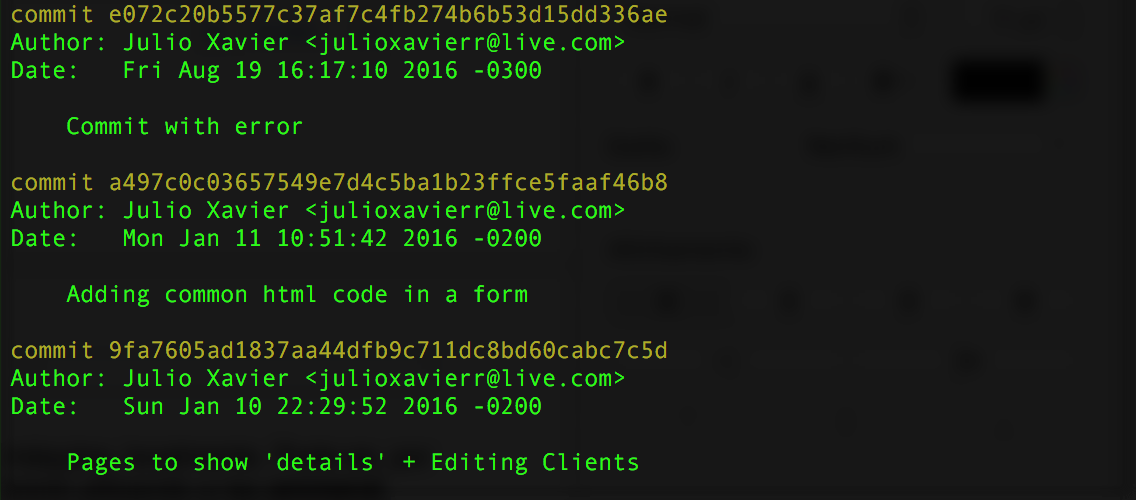
\includegraphics[width=6.25in,height=\textheight,keepaspectratio]{unidades/unidad0/../../images/git_terminal.png}

}

\caption{Git en Terminal}

\end{figure}%

Se utiliza mediante la \textbf{línea de comandos} o a través de
\textbf{interfaces gráficas} de usuario. Proporciona comandos para
realizar operaciones como:

\begin{enumerate}
\def\labelenumi{\arabic{enumi}.}
\tightlist
\item
  Inicializar un repositorio,
\item
  Realizar cambios,
\item
  Revisar historial,
\item
  Fusionar ramas,
\item
  Entre otros.
\end{enumerate}

\section{¿Para qué sirve Git? 📝}\label{para-quuxe9-sirve-git}

\begin{figure}[H]

{\centering 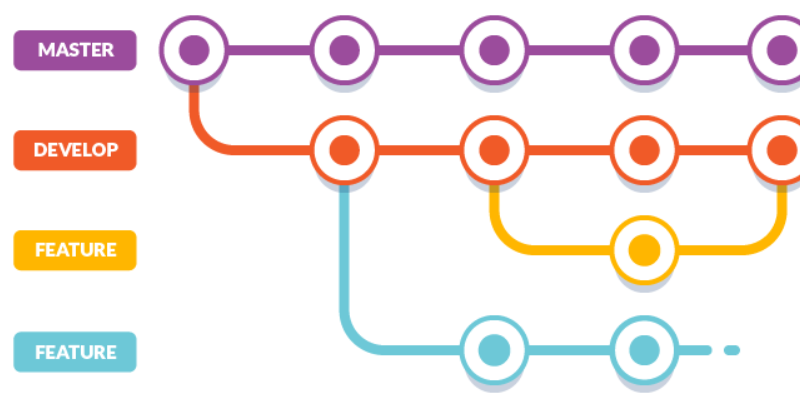
\includegraphics[width=6.25in,height=\textheight,keepaspectratio]{unidades/unidad0/../../images/seguimiento_cambios_git.png}

}

\caption{Seguimiento de Cambios con Git}

\end{figure}%

Sirve para realizar un seguimiento de los cambios en el código fuente,
coordinar el trabajo entre varios desarrolladores, revertir cambios no
deseados y mantener un historial completo de todas las modificaciones
realizadas en un proyecto.

\section{¿Por qué utilizar Git? 🤔}\label{por-quuxe9-utilizar-git}

\begin{figure}[H]

{\centering 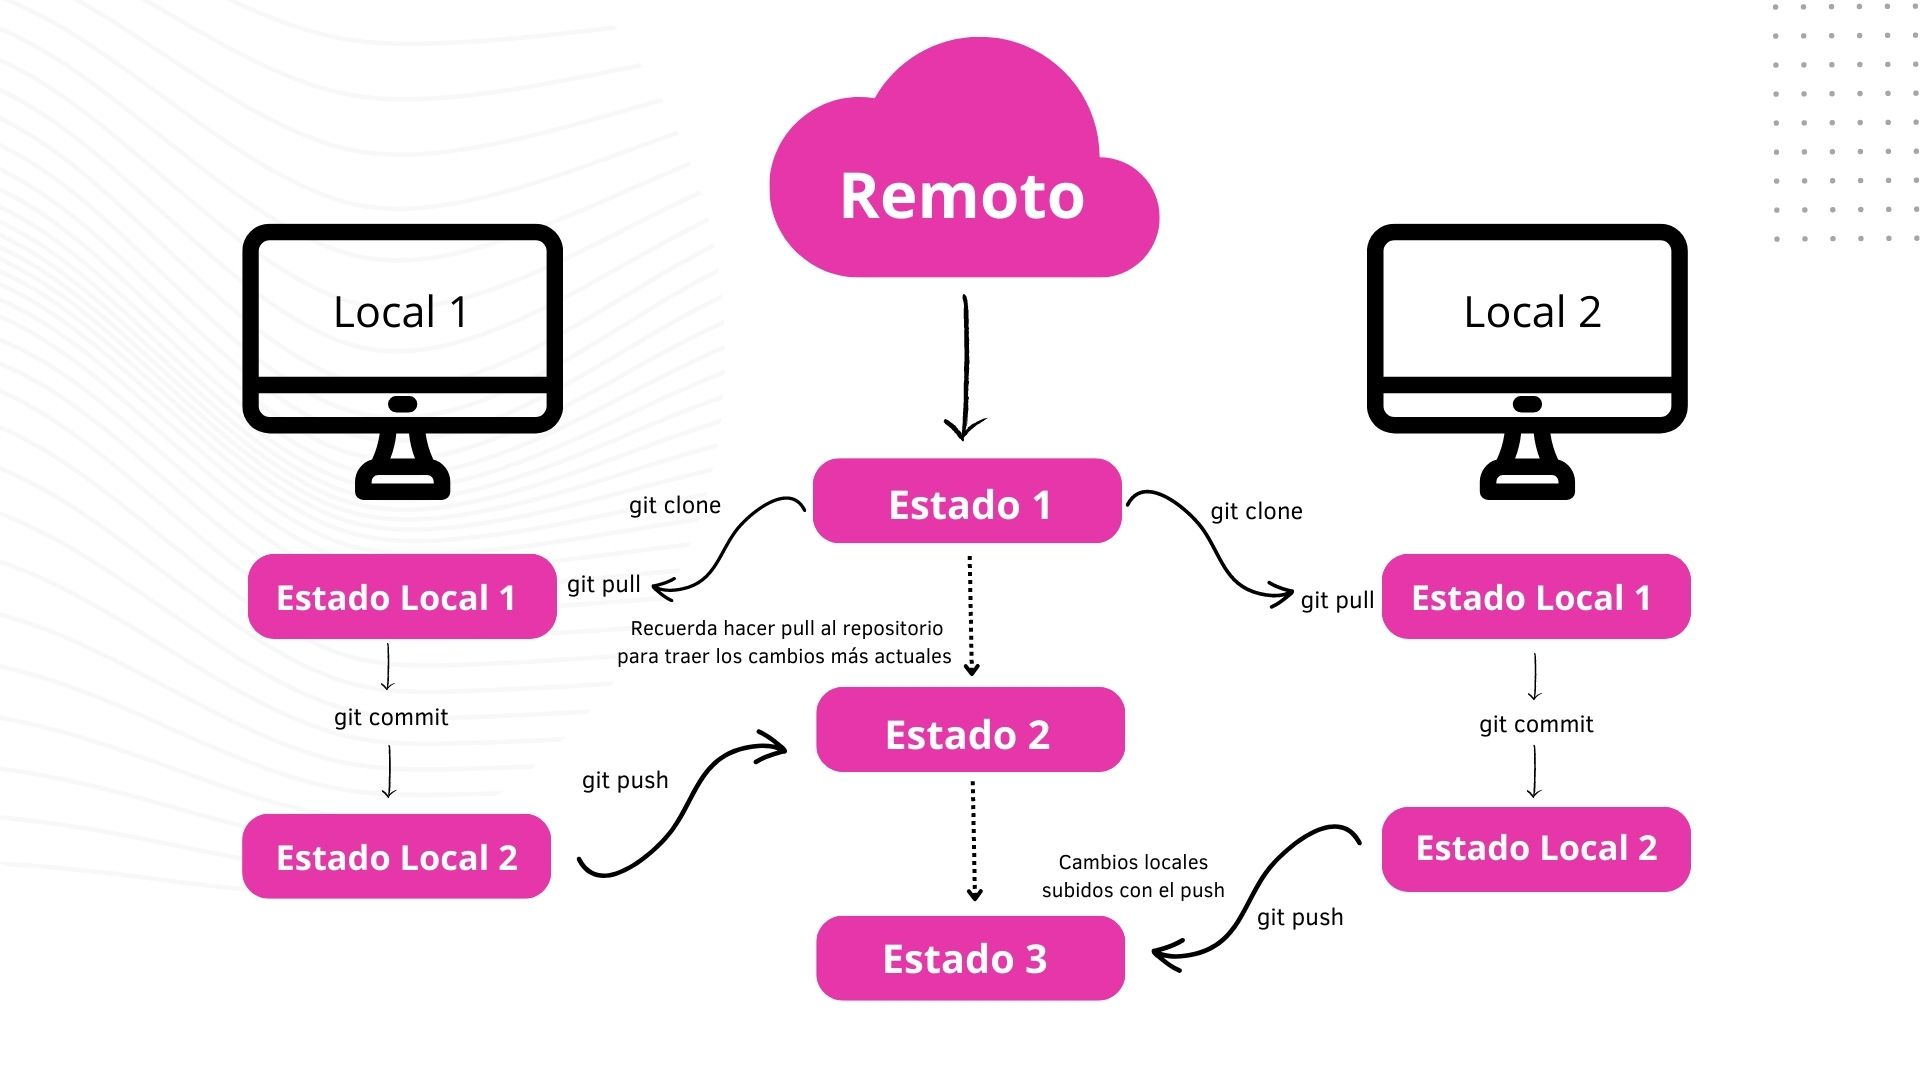
\includegraphics[width=6.25in,height=\textheight,keepaspectratio]{unidades/unidad0/../../images/ventajas_git.jpg}

}

\caption{Ventajas de Git}

\end{figure}%

Ofrece varias ventajas, como:

\begin{itemize}
\tightlist
\item
  La capacidad de trabajar de forma distribuida
\item
  La gestión eficiente de ramas para desarrollar nuevas funcionalidades
\item
  Corregir errores sin afectar la rama principal
\item
  La posibilidad de colaborar de forma efectiva con otros
  desarrolladores.
\end{itemize}

\section{¿Dónde puedo utilizar Git?
🌐}\label{duxf3nde-puedo-utilizar-git}

\begin{figure}[H]

{\centering 
\includegraphics[width=6.25in,height=\textheight,keepaspectratio]{unidades/unidad0/../../images/sistemas_operativos_git.png}

}

\caption{Git en Diferentes Sistemas Operativos}

\end{figure}%

Puede ser utilizado en cualquier sistema operativo, incluyendo Windows,
macOS y Linux. Además, es compatible con una amplia variedad de
plataformas de alojamiento de repositorios, siendo GitHub una de las más
populares.

\section{Pasos Básicos 📝}\label{pasos-buxe1sicos}

\begin{tcolorbox}[enhanced jigsaw, toptitle=1mm, titlerule=0mm, left=2mm, opacityback=0, coltitle=black, leftrule=.75mm, title=\textcolor{quarto-callout-tip-color}{\faLightbulb}\hspace{0.5em}{Tip}, bottomrule=.15mm, arc=.35mm, opacitybacktitle=0.6, bottomtitle=1mm, toprule=.15mm, colbacktitle=quarto-callout-tip-color!10!white, rightrule=.15mm, breakable, colframe=quarto-callout-tip-color-frame, colback=white]

Es recomendable tomar en cuenta una herramienta para la edición de
código, como Visual Studio Code, Sublime Text o Atom, para trabajar con
Git y GitHub de manera eficiente.

\end{tcolorbox}

\section{Instalación de Visual Studio Code
📥}\label{instalaciuxf3n-de-visual-studio-code}

\begin{figure}[H]

{\centering 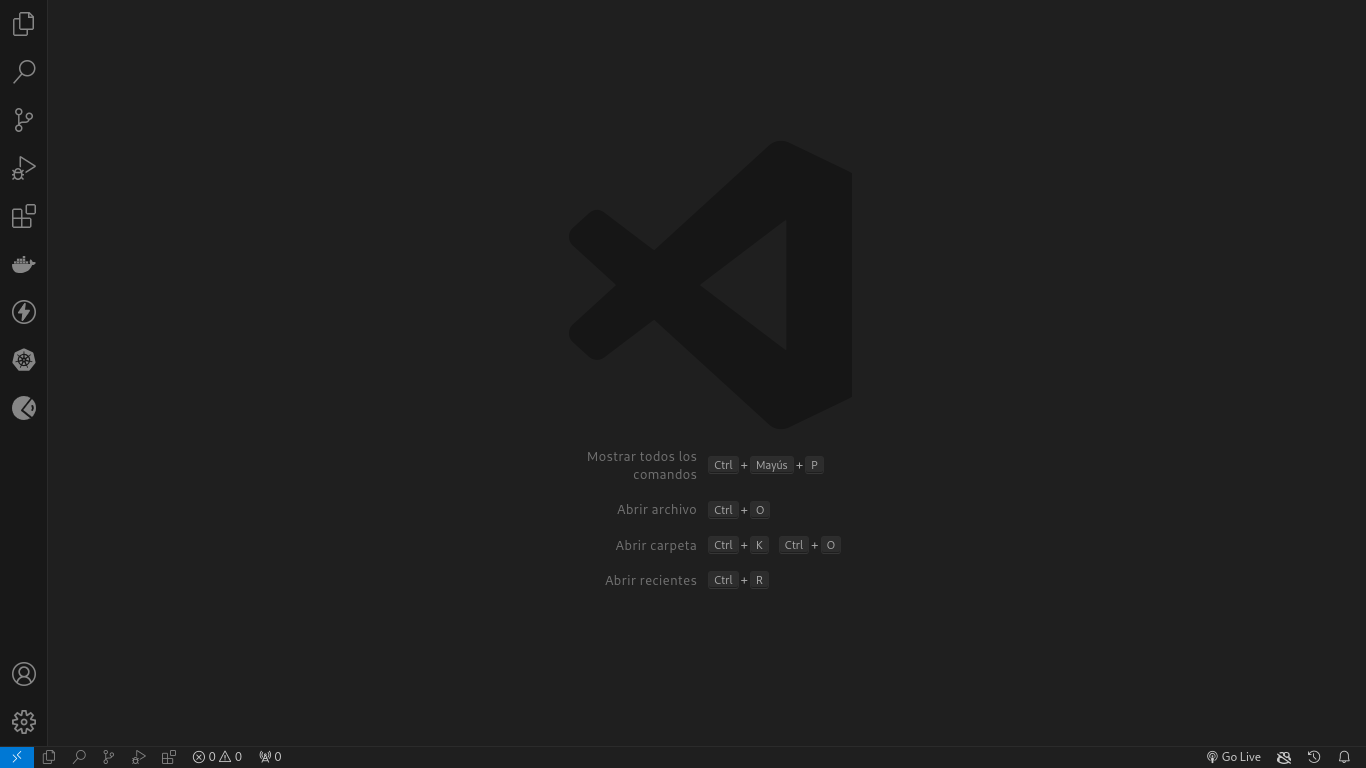
\includegraphics[width=6.25in,height=\textheight,keepaspectratio]{unidades/unidad0/../../images/vscode.png}

}

\caption{Visual Studio Code}

\end{figure}%

Si aún no tienes Visual Studio Code instalado, puedes descargarlo desde
\url{https://code.visualstudio.com/download}. Es una herramienta
gratuita y de código abierto que proporciona una interfaz amigable para
trabajar con Git y GitHub.

A continuación se presentan los pasos básicos para utilizar Git y GitHub
en un proyecto de software.

\subsection{Descarga e Instalación de Git
📥}\label{descarga-e-instalaciuxf3n-de-git}

\begin{figure}[H]

{\centering 
\includegraphics[width=6.25in,height=\textheight,keepaspectratio]{unidades/unidad0/../../images/website-git.png}

}

\caption{Git}

\end{figure}%

\begin{enumerate}
\def\labelenumi{\arabic{enumi}.}
\tightlist
\item
  Visita el sitio web oficial de Git en
  \url{https://git-scm.com/downloads}.
\item
  Descarga el instalador adecuado para tu sistema operativo y sigue las
  instrucciones de instalación.
\end{enumerate}

\subsection{Configuración 🛠️}\label{configuraciuxf3n}

\begin{figure}[H]

{\centering 
\includegraphics[width=6.25in,height=\textheight,keepaspectratio]{unidades/unidad0/../../images/git_config.png}

}

\caption{Configuración de Git}

\end{figure}%

Una vez instalado Git, es necesario configurar tu nombre de usuario y
dirección de correo electrónico. Esto se puede hacer mediante los
siguientes comandos:

\begin{Shaded}
\begin{Highlighting}[]
\FunctionTok{git}\NormalTok{ config }\AttributeTok{{-}{-}global}\NormalTok{ user.name }\StringTok{"Tu Nombre"}
\FunctionTok{git}\NormalTok{ config }\AttributeTok{{-}{-}global}\NormalTok{ user.email }\StringTok{"tu@email.com"}
\end{Highlighting}
\end{Shaded}

\subsection{Creación de un Repositorio ``helloWorld'' en Python
🐍}\label{creaciuxf3n-de-un-repositorio-helloworld-en-python}

\begin{itemize}
\tightlist
\item
  Crea una nueva carpeta para tu proyecto y ábrela en Visual Studio
  Code.
\item
  Crea un archivo Python llamado \textbf{hello\_world.py} y escribe el
  siguiente código:
\end{itemize}

\begin{Shaded}
\begin{Highlighting}[]
\KeywordTok{def}\NormalTok{ welcome\_message():}
\NormalTok{    name }\OperatorTok{=} \BuiltInTok{input}\NormalTok{(}\StringTok{"Ingrese su nombre: "}\NormalTok{)}
    \BuiltInTok{print}\NormalTok{(}\StringTok{"Bienvenio,"}\NormalTok{, name, }\StringTok{"al curso de Django y React!"}\NormalTok{)}

\ControlFlowTok{if} \VariableTok{\_\_name\_\_} \OperatorTok{==} \StringTok{"\_\_main\_\_"}\NormalTok{:}
\NormalTok{    welcome\_message()}
\end{Highlighting}
\end{Shaded}

\begin{itemize}
\tightlist
\item
  Guarda el archivo y abre una terminal en Visual Studio Code.
\item
  Inicializa un repositorio Git en la carpeta de tu proyecto con el
  siguiente comando:
\end{itemize}

\begin{Shaded}
\begin{Highlighting}[]
\FunctionTok{git}\NormalTok{ init}
\end{Highlighting}
\end{Shaded}

\begin{itemize}
\tightlist
\item
  Añade el archivo al área de preparación con:
\end{itemize}

\begin{Shaded}
\begin{Highlighting}[]
\FunctionTok{git}\NormalTok{ add hello\_world.py}
\end{Highlighting}
\end{Shaded}

\begin{itemize}
\tightlist
\item
  Realiza un commit de los cambios con un mensaje descriptivo:
\end{itemize}

\begin{Shaded}
\begin{Highlighting}[]
\FunctionTok{git}\NormalTok{ commit }\AttributeTok{{-}m} \StringTok{"Añadir archivo hello\_world.py"}
\end{Highlighting}
\end{Shaded}

\subsection{Comandos Básicos de Git
📝}\label{comandos-buxe1sicos-de-git}

\begin{itemize}
\tightlist
\item
  \textbf{git init:} Inicializa un nuevo repositorio Git.
\item
  \textbf{git add :} Añade un archivo al área de preparación.
\item
  \textbf{git commit -m ``''}: Realiza un commit de los cambios con un
  mensaje descriptivo.
\item
  \textbf{git push:} Sube los cambios al repositorio remoto.
\item
  \textbf{git pull:} Descarga cambios del repositorio remoto.
\item
  \textbf{git branch:} Lista las ramas disponibles.
\item
  \textbf{git checkout :} Cambia a una rama específica.
\item
  \textbf{git merge :} Fusiona una rama con la rama actual.
\item
  \textbf{git reset :} Descarta los cambios en un archivo.
\item
  \textbf{git diff:} Muestra las diferencias entre versiones.
\end{itemize}

\subsection{Estados en Git 📊}\label{estados-en-git}

\begin{itemize}
\tightlist
\item
  \textbf{Local:} Representa los cambios que realizas en tu repositorio
  local antes de hacer un commit. Estos cambios están únicamente en tu
  máquina.
\item
  \textbf{Staging:} Indica los cambios que has añadido al área de
  preparación con el comando \texttt{git\ add}. Estos cambios están
  listos para ser confirmados en el próximo commit.
\item
  \textbf{Commit:} Son los cambios que has confirmado en tu repositorio
  local con el comando \texttt{git\ commit}. Estos cambios se han
  guardado de manera permanente en tu repositorio local.
\item
  \textbf{Server:} Son los cambios que has subido al repositorio remoto
  con el comando \texttt{git\ push}. Estos cambios están disponibles
  para otros colaboradores del proyecto.
\end{itemize}

\begin{center}\rule{0.5\linewidth}{0.5pt}\end{center}

\chapter{Tutorial: Moviendo Cambios entre Estados en Git
📝}\label{tutorial-moviendo-cambios-entre-estados-en-git}

\section{Introducción}\label{introducciuxf3n}

En este tutorial, aprenderemos a utilizar Git para gestionar cambios en
nuestro proyecto y moverlos entre diferentes estados. Utilizaremos un
ejemplo práctico para comprender mejor estos conceptos.

\begin{Shaded}
\begin{Highlighting}[]
\KeywordTok{def}\NormalTok{ welcome\_message():}
\NormalTok{    name }\OperatorTok{=} \BuiltInTok{input}\NormalTok{(}\StringTok{"Ingrese su nombre: "}\NormalTok{)}
    \BuiltInTok{print}\NormalTok{(}\StringTok{"Bienvenio,"}\NormalTok{, name, }\StringTok{"al curso de Django y React!"}\NormalTok{)}

\ControlFlowTok{if} \VariableTok{\_\_name\_\_} \OperatorTok{==} \StringTok{"\_\_main\_\_"}\NormalTok{:}
\NormalTok{    welcome\_message()}
\end{Highlighting}
\end{Shaded}

\section{Sección 1: Modificar Archivos en el
Repositorio}\label{secciuxf3n-1-modificar-archivos-en-el-repositorio}

En esta sección, aprenderemos cómo realizar cambios en nuestros archivos
y reflejarlos en Git.

\section{Mover Cambios de Local a
Staging:}\label{mover-cambios-de-local-a-staging}

\begin{enumerate}
\def\labelenumi{\arabic{enumi}.}
\tightlist
\item
  Abre el archivo \textbf{hello\_world.py} en Visual Studio Code.
\item
  Modifica el mensaje de bienvenida a ``Bienvenido'' en lugar de
  ``Bienvenio''.
\item
  Guarda los cambios y abre una terminal en Visual Studio Code.
\end{enumerate}

Hemos corregido un error en nuestro archivo y queremos reflejarlo en
Git.

\begin{Shaded}
\begin{Highlighting}[]
\ExtensionTok{def}\NormalTok{ welcome\_message}\ErrorTok{(}\KeywordTok{)}\BuiltInTok{:}
    \ExtensionTok{name}\NormalTok{ = input}\ErrorTok{(}\StringTok{"Ingrese su nombre: "}\KeywordTok{)}
    \ExtensionTok{print}\ErrorTok{(}\StringTok{"Bienvenido,"}\ExtensionTok{,}\NormalTok{ name, }\StringTok{"al curso de Django y React!"}\KeywordTok{)}

\ControlFlowTok{if} \ExtensionTok{\_\_name\_\_}\NormalTok{ == }\StringTok{"\_\_main\_\_"}\NormalTok{:}
    \FunctionTok{welcome\_message()}
\end{Highlighting}
\end{Shaded}

\section{Agregar Cambios de Local a
Staging:}\label{agregar-cambios-de-local-a-staging}

\begin{Shaded}
\begin{Highlighting}[]
\FunctionTok{git}\NormalTok{ add hello\_world.py}
\end{Highlighting}
\end{Shaded}

Hemos añadido los cambios al área de preparación y están listos para ser
confirmados en el próximo commit.

\section{Sección 2: Confirmar Cambios en un
Commit}\label{secciuxf3n-2-confirmar-cambios-en-un-commit}

En esta sección, aprenderemos cómo confirmar los cambios en un commit y
guardarlos de manera permanente en nuestro repositorio.

\section{Mover Cambios de Staging a
Commit:}\label{mover-cambios-de-staging-a-commit}

\begin{Shaded}
\begin{Highlighting}[]
\FunctionTok{git}\NormalTok{ commit }\AttributeTok{{-}m} \StringTok{"Corregir mensaje de bienvenida"}
\end{Highlighting}
\end{Shaded}

Hemos confirmado los cambios en un commit con un mensaje descriptivo.

\section{Sección 3: Creación y Fusión de
Ramas}\label{secciuxf3n-3-creaciuxf3n-y-fusiuxf3n-de-ramas}

En esta sección, aprenderemos cómo crear y fusionar ramas en Git para
desarrollar nuevas funcionalidades de forma aislada.

\section{Crear una Nueva Rama:}\label{crear-una-nueva-rama}

\begin{Shaded}
\begin{Highlighting}[]
\FunctionTok{git}\NormalTok{ branch feature}
\end{Highlighting}
\end{Shaded}

Hemos creado una nueva rama llamada ``feature'' para desarrollar una
nueva funcionalidad.

\section{Implementar Funcionalidades en la
Rama:}\label{implementar-funcionalidades-en-la-rama}

\begin{enumerate}
\def\labelenumi{\arabic{enumi}.}
\tightlist
\item
  Abre el archivo \textbf{hello\_world.py} en Visual Studio Code.
\item
  Añade una nueva función para mostrar un mensaje de despedida.
\item
  Guarda los cambios y abre una terminal en Visual Studio Code.
\item
  Añade los cambios al área de preparación y confírmalos en un commit.
\item
  Cambia a la rama principal con \texttt{git\ checkout\ main}.
\end{enumerate}

\section{Fusionar Ramas con la Rama
Principal:}\label{fusionar-ramas-con-la-rama-principal}

\begin{Shaded}
\begin{Highlighting}[]
\FunctionTok{git}\NormalTok{ merge feature}
\end{Highlighting}
\end{Shaded}

Hemos fusionado la rama ``feature'' con la rama principal y añadido la
nueva funcionalidad al proyecto.

\section{Sección 4: Revertir Cambios en un
Archivo}\label{secciuxf3n-4-revertir-cambios-en-un-archivo}

En esta sección, aprenderemos cómo revertir cambios en un archivo y
deshacerlos en Git.

\section{Revertir Cambios en un
Archivo:}\label{revertir-cambios-en-un-archivo}

\begin{Shaded}
\begin{Highlighting}[]
\FunctionTok{git}\NormalTok{ reset hello\_world.py}
\end{Highlighting}
\end{Shaded}

Hemos revertido los cambios en el archivo \textbf{hello\_world.py} y
deshecho las modificaciones realizadas.

\section{Conclusión}\label{conclusiuxf3n}

En este tutorial, hemos aprendido a gestionar cambios en nuestro
proyecto y moverlos entre diferentes estados en Git. Estos conceptos son
fundamentales para trabajar de forma eficiente en proyectos de software
y colaborar con otros desarrolladores.

\chapter{Asignación}\label{asignaciuxf3n}

\href{https://classroom.github.com/a/o-qydr2W}{Hello World!}

Este proyecto de ejemplo está escrito en Python y se prueba con pytest.

\textbf{La Asignación}

Las pruebas están fallando en este momento porque el método no está
devolviendo la cadena correcta. Corrige el código del archivo
\textbf{hello.py} para que las pruebas sean exitosas, debe devolver la
cadena correcta \textbf{``Hello World!''}x

El comando de ejecución del test es:

\begin{Shaded}
\begin{Highlighting}[]
\ExtensionTok{pytest}\NormalTok{ test\_hello.py}
\end{Highlighting}
\end{Shaded}

¡Mucha suerte!

\chapter{GitHub Classroom 📒}\label{github-classroom}

\begin{figure}[H]

{\centering 
\includegraphics[width=1.04167in,height=\textheight,keepaspectratio]{unidades/unidad0/../../images/github classroom.png}

}

\caption{Github Classroom}

\end{figure}%

GitHub Classroom es una herramienta poderosa que facilita la gestión de
tareas y asignaciones en GitHub, especialmente diseñada para entornos
educativos.

\section{¿Qué es GitHub Classroom? 🤔}\label{quuxe9-es-github-classroom}

\begin{figure}[H]

{\centering 
\includegraphics[width=4.16667in,height=\textheight,keepaspectratio]{unidades/unidad0/../../images/github-classroom-ventana.jpg}

}

\caption{Github Classroom Windows}

\end{figure}%

GitHub Classroom es una extensión de GitHub que permite a los profesores
crear y gestionar asignaciones utilizando repositorios de GitHub.
Proporciona una forma organizada y eficiente de distribuir tareas a los
estudiantes, recopilar y revisar su trabajo, y proporcionar
retroalimentación.

\subsection{Funcionalidades Principales
⚙️}\label{funcionalidades-principales}

\textbf{Creación de Asignaciones:} Los profesores pueden crear tareas y
asignaciones directamente desde GitHub Classroom, proporcionando
instrucciones detalladas y estableciendo criterios de evaluación.

\textbf{Distribución Automatizada:} Una vez que se crea una asignación,
GitHub Classroom genera automáticamente repositorios privados para cada
estudiante o equipo, basándose en una plantilla predefinida.

\textbf{Seguimiento de Progreso:} Los profesores pueden realizar un
seguimiento del progreso de los estudiantes y revisar sus contribuciones
a través de solicitudes de extracción (pull requests) y comentarios en
el código.

\textbf{Revisión y Retroalimentación:} Los estudiantes envían sus
trabajos a través de solicitudes de extracción, lo que permite a los
profesores revisar y proporcionar retroalimentación específica sobre su
código.

\section{Ejemplo Práctico}\label{ejemplo-pruxe1ctico}

\subsection{Creación de una Asignación en GitHub Classroom
📒}\label{creaciuxf3n-de-una-asignaciuxf3n-en-github-classroom}

\textbf{Iniciar Sesión:} Ingresa a GitHub Classroom con tu cuenta de
GitHub y selecciona la opción para crear una nueva asignación.

\begin{center}
\pandocbounded{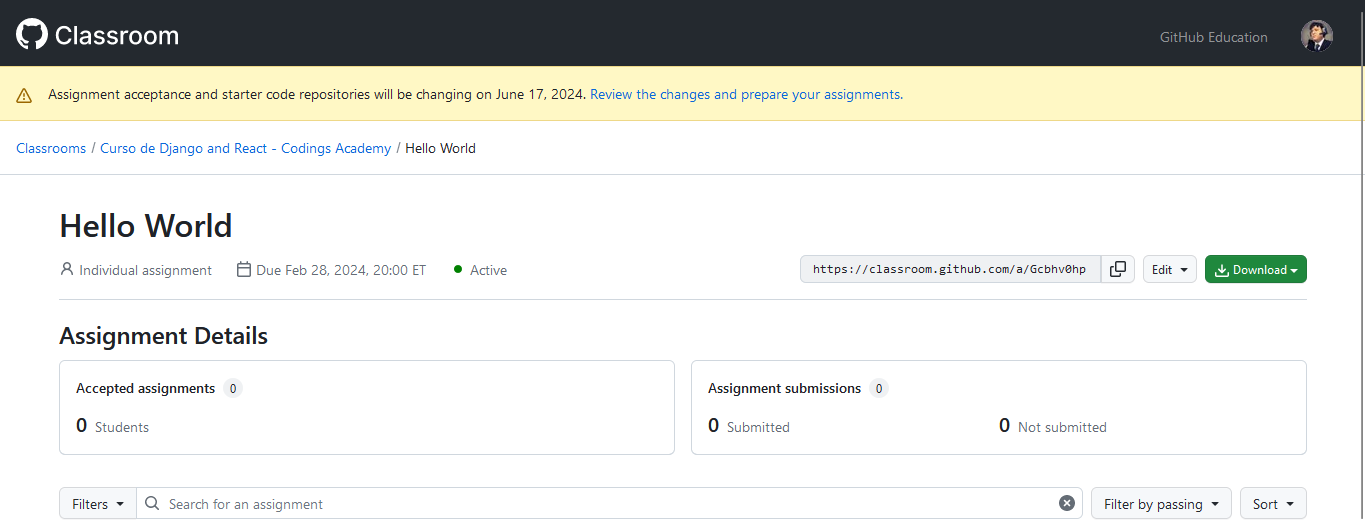
\includegraphics[keepaspectratio]{unidades/unidad0/images/paste-2.png}}
\end{center}

\textbf{Definir la Tarea:} Proporciona instrucciones claras y detalladas
sobre la tarea, incluyendo cualquier código base o recursos necesarios.
Establece los criterios de evaluación para guiar a los estudiantes.

\begin{center}
\pandocbounded{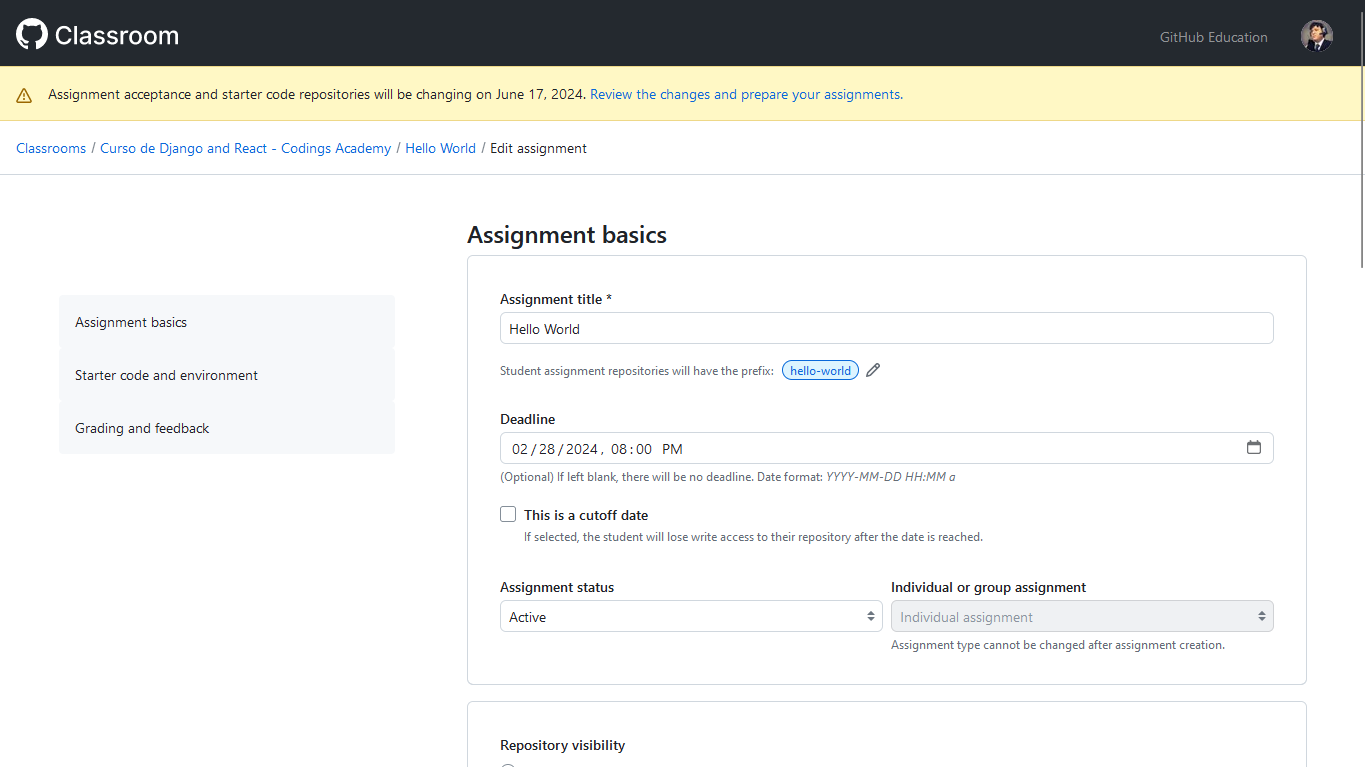
\includegraphics[keepaspectratio]{unidades/unidad0/images/paste-1.png}}
\end{center}

\textbf{Configurar la Plantilla:} Selecciona una plantilla de
repositorio existente o crea una nueva plantilla que servirá como base
para los repositorios de los estudiantes.

\begin{center}
\pandocbounded{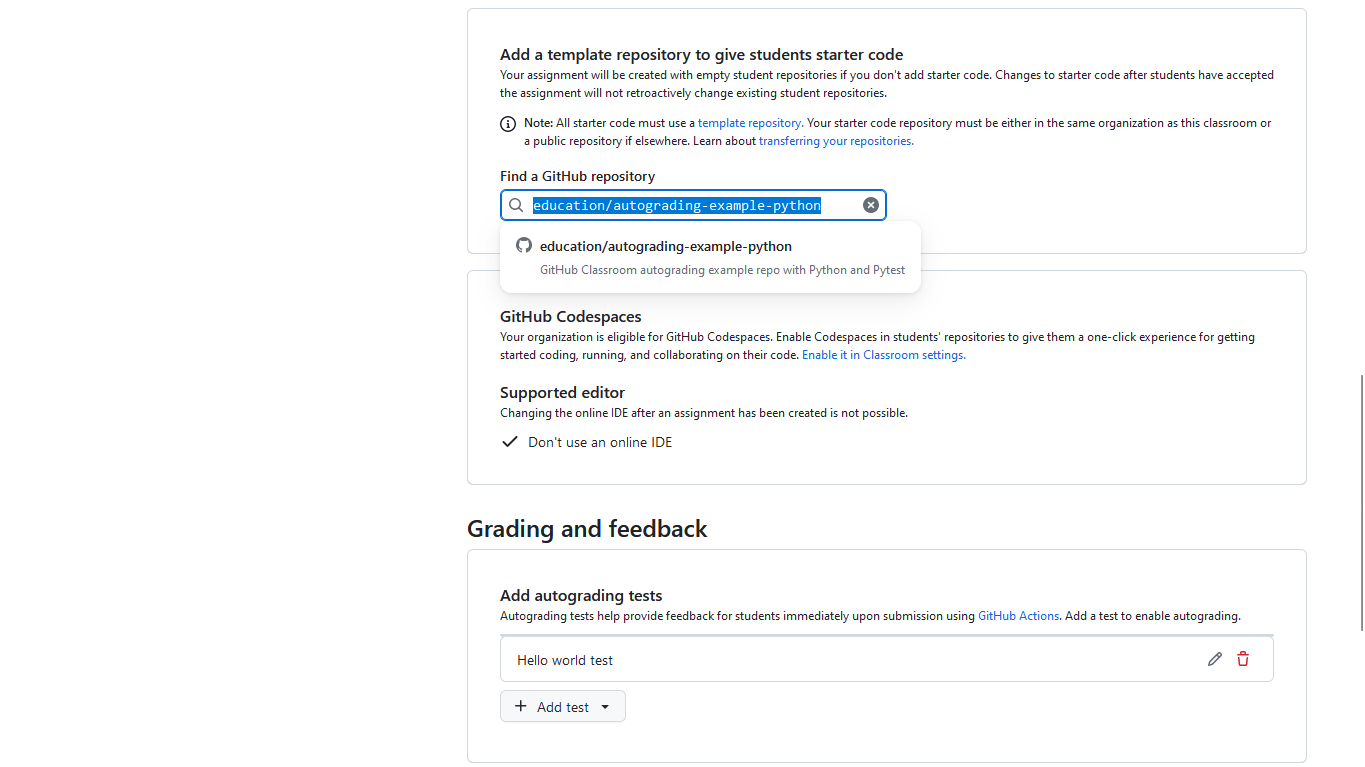
\includegraphics[keepaspectratio]{unidades/unidad0/images/paste-3.png}}
\end{center}

\textbf{Distribuir la Asignación:} Una vez configurada la asignación,
comparte el enlace generado con tus estudiantes para que puedan acceder
a sus repositorios privados.

\begin{center}
\pandocbounded{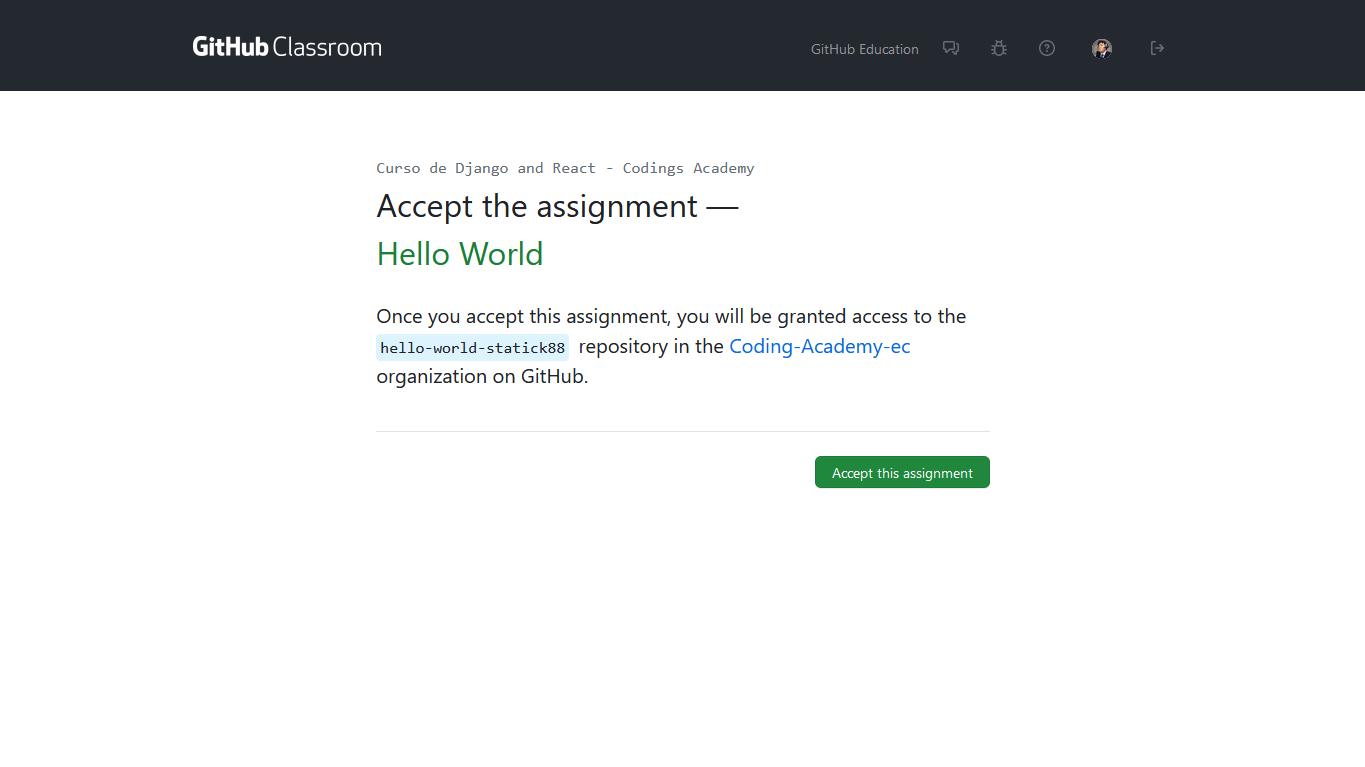
\includegraphics[keepaspectratio]{unidades/unidad0/images/paste-4.png}}
\end{center}

\section{Trabajo de los Estudiantes
🧑‍💻}\label{trabajo-de-los-estudiantes}

\textbf{Aceptar la Asignación:} Los estudiantes reciben el enlace de la
asignación y aceptan la tarea, lo que les permite crear un repositorio
privado basado en la plantilla proporcionada.

\begin{center}
\pandocbounded{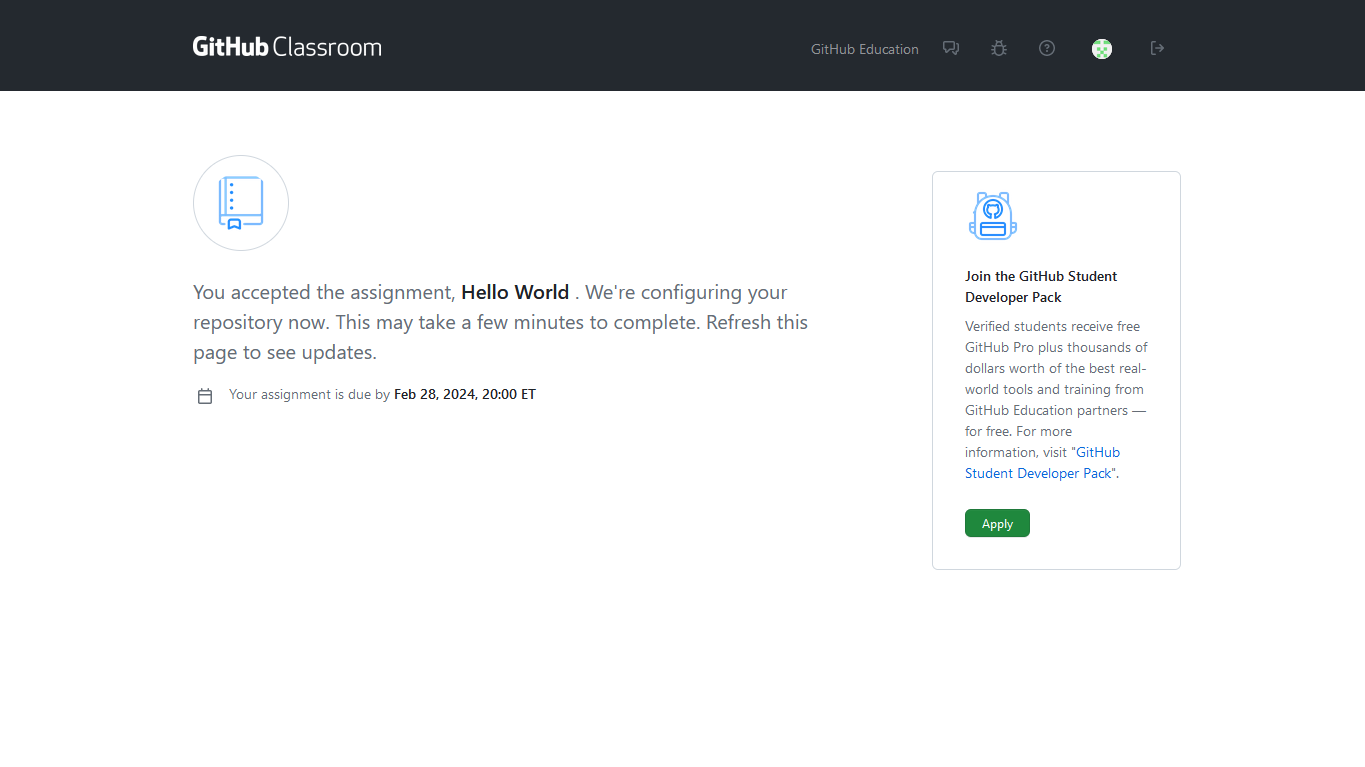
\includegraphics[keepaspectratio]{unidades/unidad0/images/paste-6.png}}
\end{center}

\textbf{Actualizar el Navegador:} Los estudiantes actualizan su
navegador para ver el nuevo repositorio creado en su cuenta de GitHub.

\begin{center}
\pandocbounded{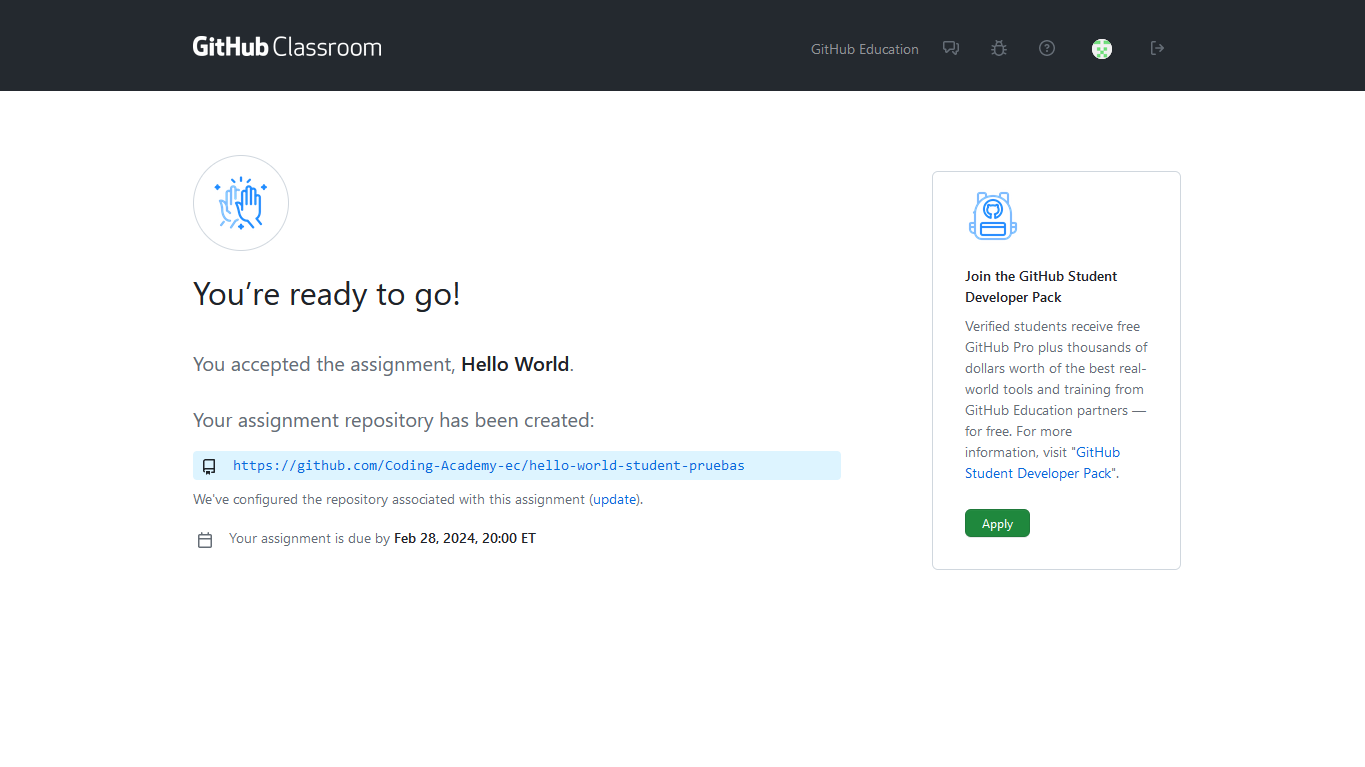
\includegraphics[keepaspectratio]{unidades/unidad0/images/paste-8.png}}
\end{center}

\textbf{Clonar el Repositorio:} Los estudiantes clonan el repositorio
asignado en su computadora local utilizando el enlace proporcionado.

\begin{center}
\pandocbounded{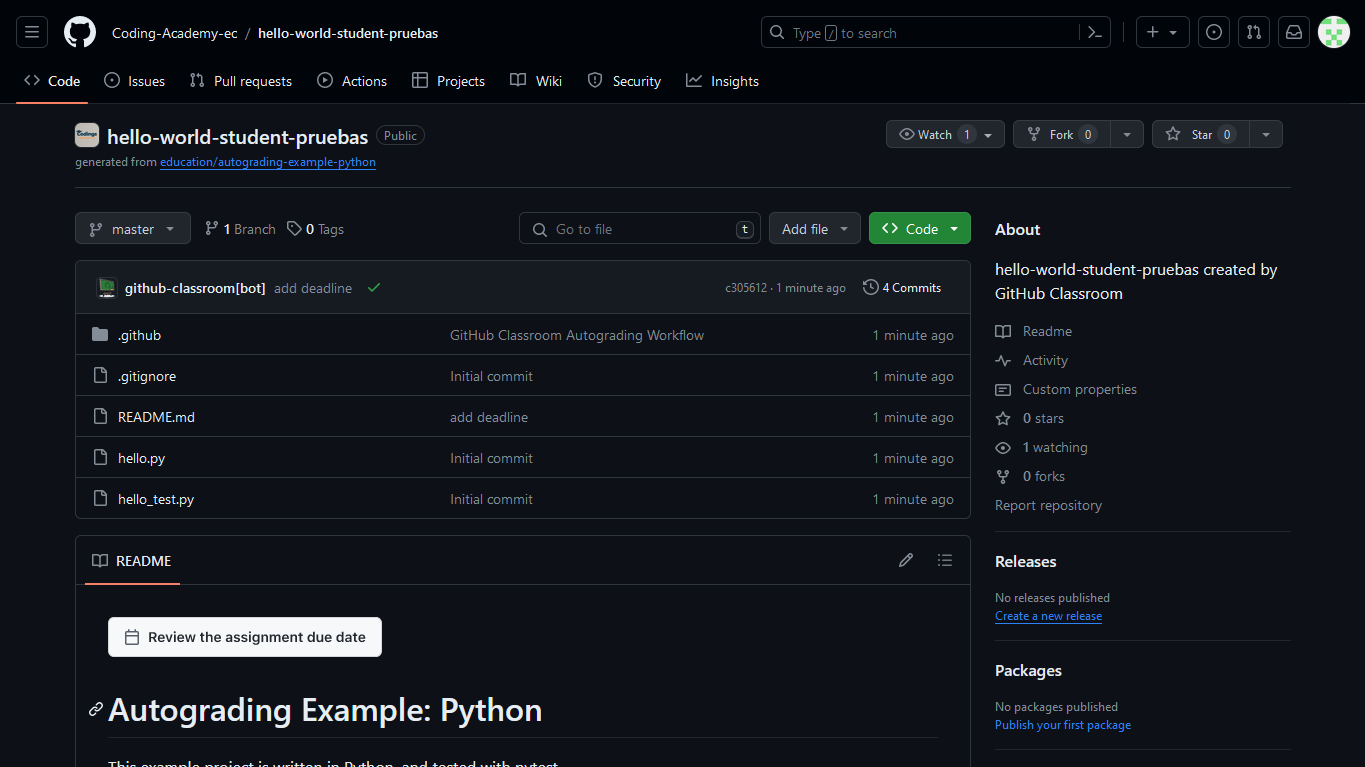
\includegraphics[keepaspectratio]{unidades/unidad0/images/paste-9.png}}
\end{center}

Utilizar el comando git clone: Aplique el comando git clone para clonar
el repositorio en su computadora local.

\begin{Shaded}
\begin{Highlighting}[]
\FunctionTok{git}\NormalTok{ clone }\OperatorTok{\textless{}}\NormalTok{enlace{-}del{-}repositorio}\OperatorTok{\textgreater{}}
\end{Highlighting}
\end{Shaded}

\begin{center}
\pandocbounded{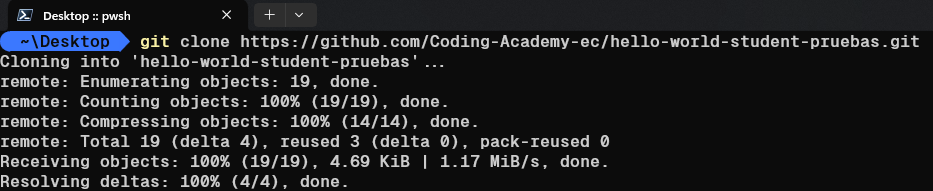
\includegraphics[keepaspectratio]{unidades/unidad0/images/paste-10.png}}
\end{center}

\textbf{Desarrollar la Tarea:} Los estudiantes trabajan en la tarea,
realizando los cambios necesarios y realizando commits de manera regular
para mantener un historial de su trabajo.

\begin{tcolorbox}[enhanced jigsaw, toptitle=1mm, titlerule=0mm, left=2mm, opacityback=0, coltitle=black, leftrule=.75mm, title=\textcolor{quarto-callout-tip-color}{\faLightbulb}\hspace{0.5em}{Tip}, bottomrule=.15mm, arc=.35mm, opacitybacktitle=0.6, bottomtitle=1mm, toprule=.15mm, colbacktitle=quarto-callout-tip-color!10!white, rightrule=.15mm, breakable, colframe=quarto-callout-tip-color-frame, colback=white]

Puedes probar el test incorporado con el comando \texttt{pytest} en la
terminal, para verificar que el código cumple con los requerimientos

\end{tcolorbox}

\begin{Shaded}
\begin{Highlighting}[]
\ExtensionTok{pytest}
\end{Highlighting}
\end{Shaded}

Una vez desarrollado el código de acuerdo a la asignación en local
deberían pasar el o los test

\begin{center}
\pandocbounded{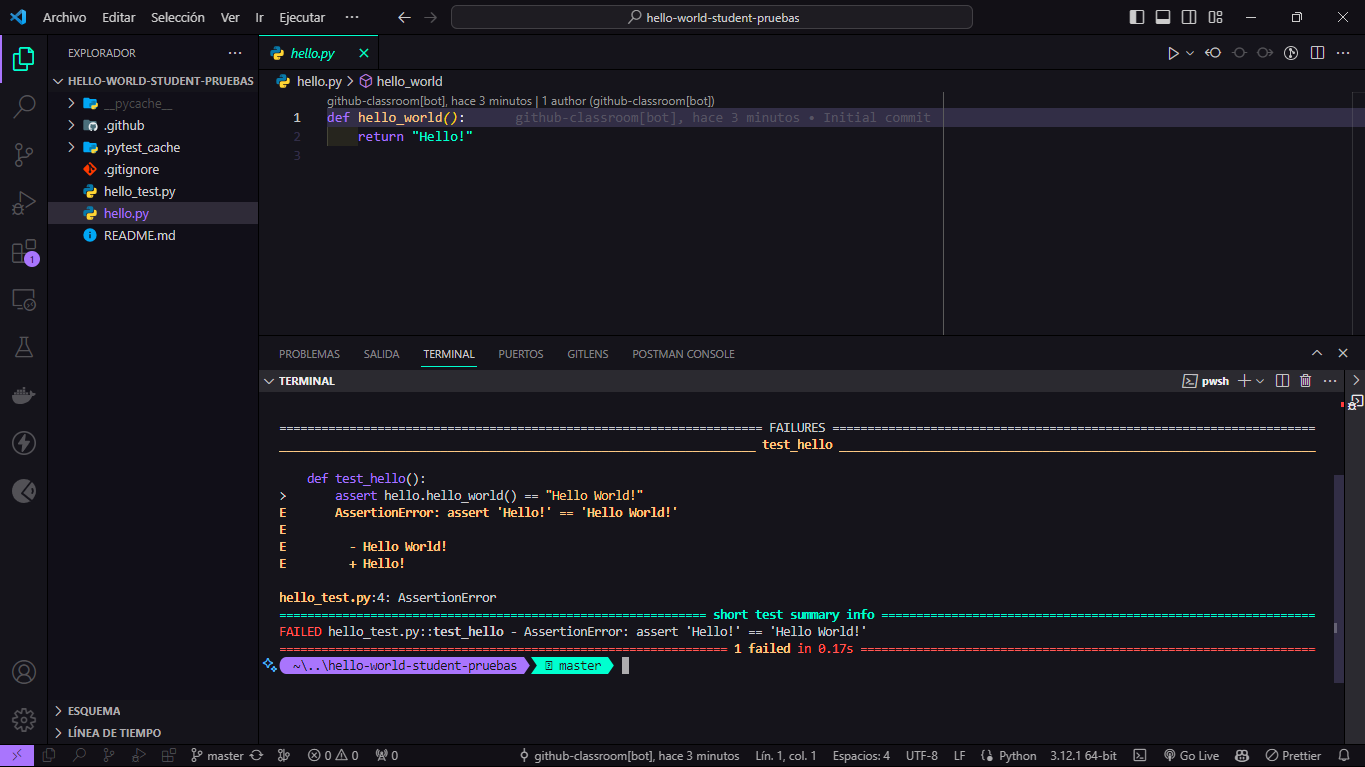
\includegraphics[keepaspectratio]{unidades/unidad0/images/paste-11.png}}
\end{center}

\textbf{Enviar la Solicitud de Extracción:} Una vez completada la tarea,
los estudiantes envían una solicitud de extracción desde su rama hacia
la rama principal del repositorio, solicitando la revisión del profesor.

\begin{center}
\pandocbounded{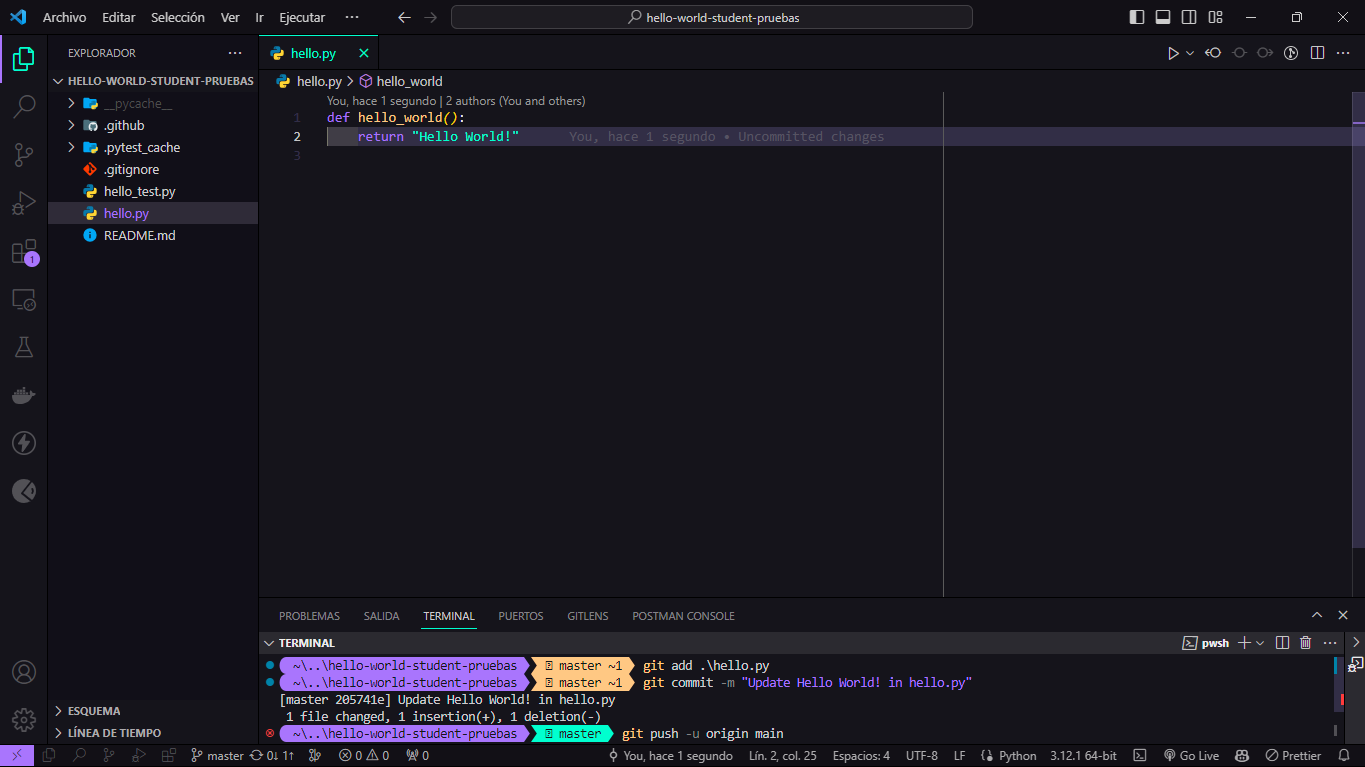
\includegraphics[keepaspectratio]{unidades/unidad0/images/paste-12.png}}
\end{center}

Una vez realizado el \texttt{push} se envía al respositorio principal y
se ejecutan los test en Github

\begin{tcolorbox}[enhanced jigsaw, toptitle=1mm, titlerule=0mm, left=2mm, opacityback=0, coltitle=black, leftrule=.75mm, title=\textcolor{quarto-callout-tip-color}{\faLightbulb}\hspace{0.5em}{Tip}, bottomrule=.15mm, arc=.35mm, opacitybacktitle=0.6, bottomtitle=1mm, toprule=.15mm, colbacktitle=quarto-callout-tip-color!10!white, rightrule=.15mm, breakable, colframe=quarto-callout-tip-color-frame, colback=white]

Se recomienda hacer las pruebas en local antes de enviar los cambios al
respositorio en Github

\end{tcolorbox}

\begin{center}
\pandocbounded{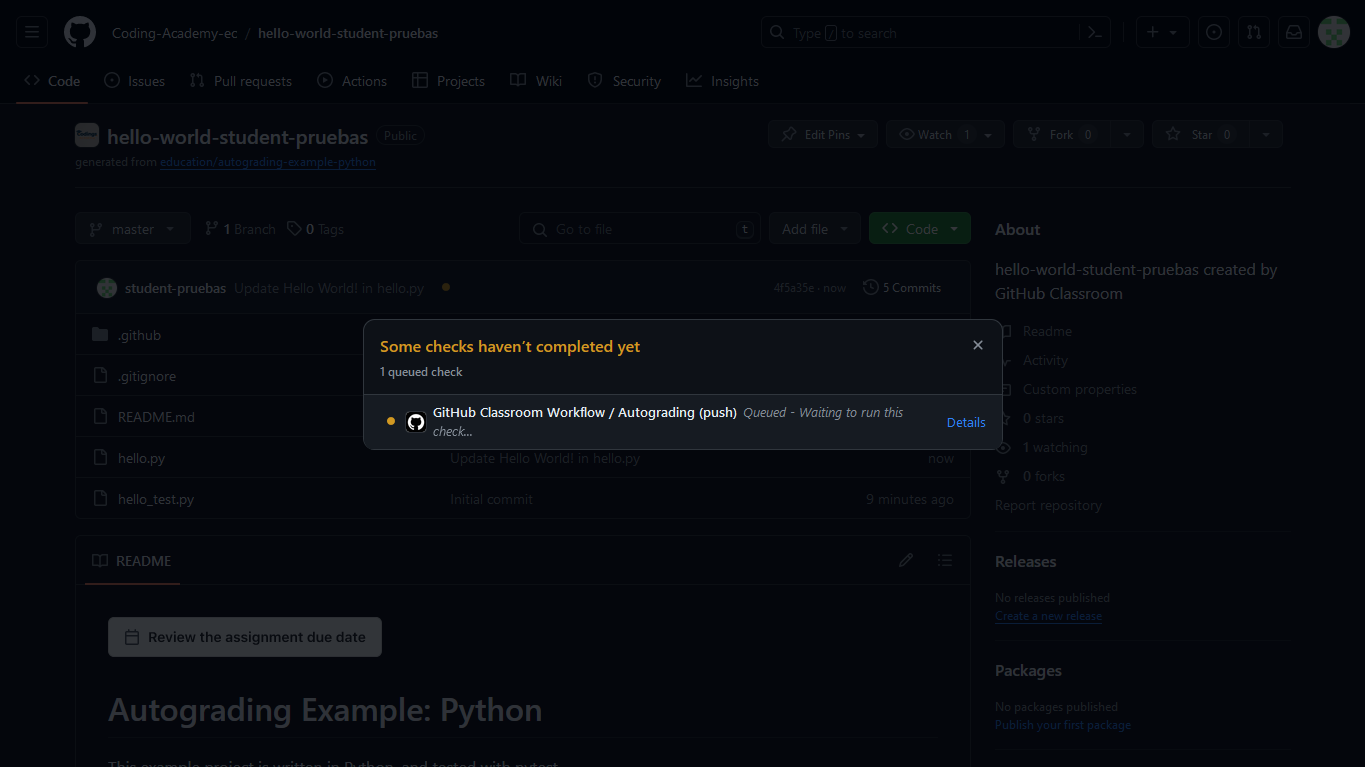
\includegraphics[keepaspectratio]{unidades/unidad0/images/paste-13.png}}
\end{center}

Este Action lo que hace es evaluar los cambios realizados

\begin{center}
\pandocbounded{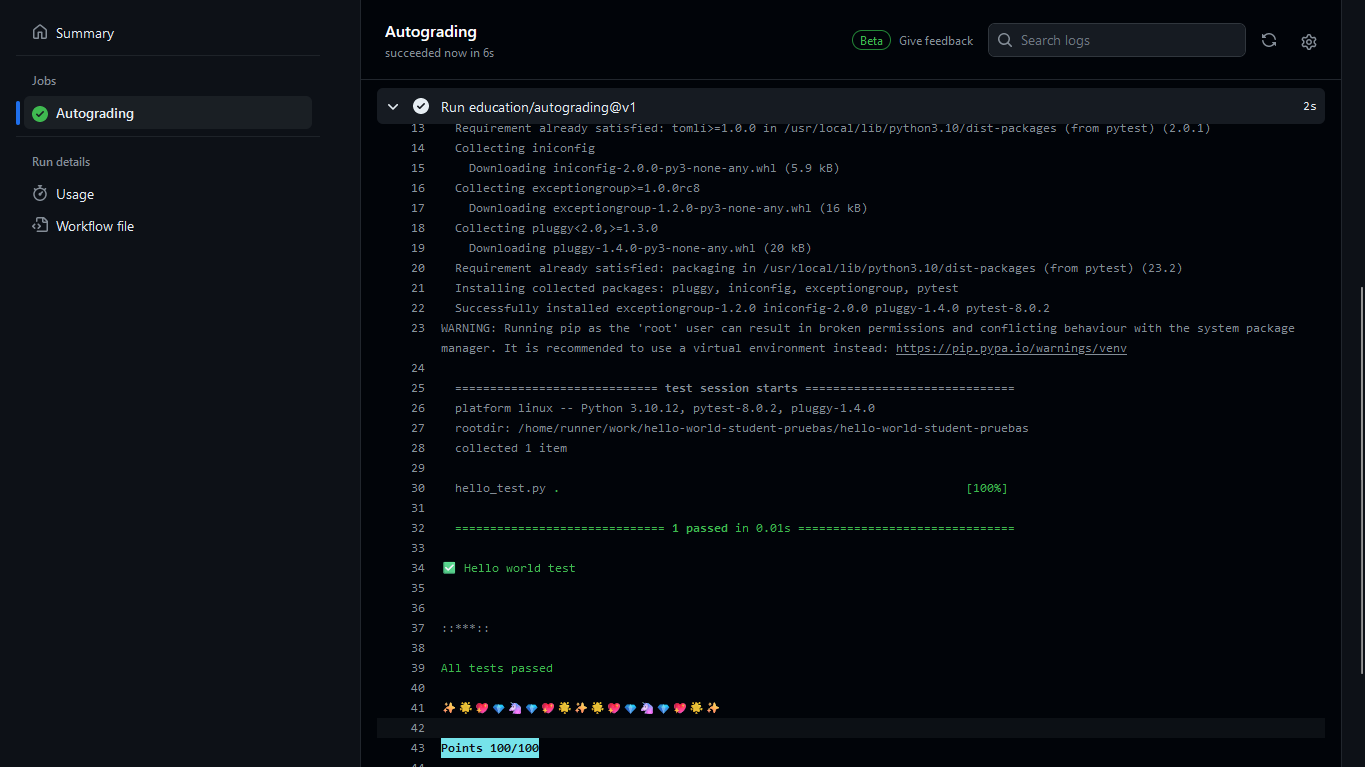
\includegraphics[keepaspectratio]{unidades/unidad0/images/paste-14.png}}
\end{center}

\begin{tcolorbox}[enhanced jigsaw, toptitle=1mm, titlerule=0mm, left=2mm, opacityback=0, coltitle=black, leftrule=.75mm, title=\textcolor{quarto-callout-tip-color}{\faLightbulb}\hspace{0.5em}{Tip}, bottomrule=.15mm, arc=.35mm, opacitybacktitle=0.6, bottomtitle=1mm, toprule=.15mm, colbacktitle=quarto-callout-tip-color!10!white, rightrule=.15mm, breakable, colframe=quarto-callout-tip-color-frame, colback=white]

Se recomienda hacer las pruebas en local antes de enviar los cambios al
respositorio en Github

\end{tcolorbox}

\textbf{Revisión y Retroalimentación:} Los profesores revisan las
solicitudes de extracción, proporcionan comentarios sobre el código y
evalúan el trabajo de los estudiantes según los criterios establecidos.

\begin{center}
\pandocbounded{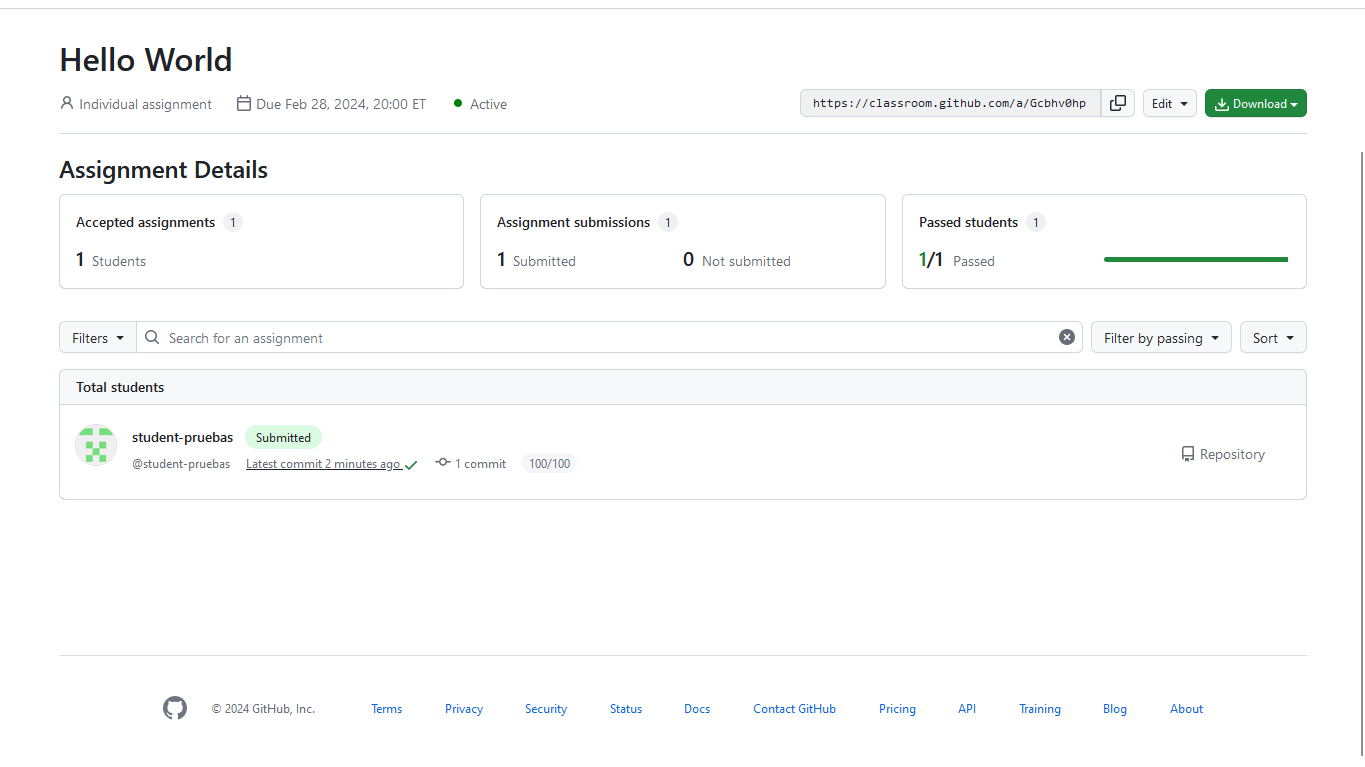
\includegraphics[keepaspectratio]{unidades/unidad0/images/paste-15.png}}
\end{center}

\begin{tcolorbox}[enhanced jigsaw, toptitle=1mm, titlerule=0mm, left=2mm, opacityback=0, coltitle=black, leftrule=.75mm, title=\textcolor{quarto-callout-tip-color}{\faLightbulb}\hspace{0.5em}{Tip}, bottomrule=.15mm, arc=.35mm, opacitybacktitle=0.6, bottomtitle=1mm, toprule=.15mm, colbacktitle=quarto-callout-tip-color!10!white, rightrule=.15mm, breakable, colframe=quarto-callout-tip-color-frame, colback=white]

\textbf{GitHub Classroom} ofrece una manera eficiente y organizada de
administrar tareas y asignaciones en entornos educativos, fomentando la
colaboración, el aprendizaje y la retroalimentación efectiva entre
profesores y estudiantes.

\end{tcolorbox}

\part{Unidad 1: Introducción e Instalaciones Necesarias}

\chapter{Introducción e Instalaciones
Necesarias.}\label{introducciuxf3n-e-instalaciones-necesarias.}

\begin{figure}[H]

{\centering \pandocbounded{
\includegraphics[keepaspectratio]{unidades/unidad1/images/logica_programacion.jpeg}}

}

\caption{Lógica de la Programación}

\end{figure}%

En este Bootcamp aprenderemos las bases y fundamentos necesarios del
desarrollo web fullstack, esto es desde el frontend hasta el backend.

Para ello, utilizaremos Python como lenguaje de programación principal,
y Django y FastAPI como frameworks para el desarrollo de aplicaciones
web.

Por otra parte esta tambien el frontend, donde utilizaremos HTML, CSS y
JavaScript para el desarrollo de interfaces de usuario, aprenderemos
acerca de Node.js y React.js para el desarrollo de aplicaciones web del
lado del cliente.

Sin embargo antes de empezar con el desarrollo web, es necesario tener
una base sólida en programación, por lo que en este primer módulo
aprenderemos acerca de Python, un lenguaje de programación de alto
nivel, interpretado y orientado a objetos.

Por otra parte es necesario saber que cualquier lenguaje de programación
no es suficiente para poder desarrollar sistemas que permitan resolver
problemas del diario vivir, es necesario tener un entorno de desarrollo
adecuado, por lo que en este módulo también aprenderemos acerca de los
entornos de desarrollo que podemos utilizar para programar en Python.

En este módulo aprenderemos acerca de los siguientes temas:

\begin{itemize}
\item
  Introducción General a la Programación
\item
  Instalación de Python
\item
  Uso de REPL, PEP 8 y Zen de Python
\item
  Entornos de Desarrollo
\end{itemize}

\section{Introducción General a la
Programación}\label{introducciuxf3n-general-a-la-programaciuxf3n}

Si más preámbulos, empecemos con la introducción general a la
programación.

Es el proceso de diseñar e implementar un programa de computadora, es
decir, un conjunto de instrucciones que le dicen a una computadora qué
hacer.

Es una habilidad muy valiosa en el mundo actual, ya que la mayoría de
las tareas que realizamos a diario involucran el uso de computadoras y
software.

Nos permite automatizar tareas, resolver problemas de manera eficiente y
crear aplicaciones y sistemas que nos ayudan en nuestra vida diaria.

En este módulo aprenderemos los fundamentos de la programación
utilizando Python, un lenguaje de programación de alto nivel,
interpretado y orientado a objetos.

Antes de introducirnos en el aprendizaje del lenguaje de programación,
es importante conocer que debemos desarrollar la \textbf{lógica de la
prograamción}, es decir, la habilidad de pensar de manera lógica y
estructurada para resolver problemas de manera eficiente.

Analicemos el siguiente problema para entender la importancia de la
lógica de programación:

\begin{itemize}
\tightlist
\item
  \textbf{Problema}: Supongamos que queremos escribir un programa que
  imprima los números del 1 al 10.
\end{itemize}

¿Cómo resolverías este problema?

Una posible solución sería escribir un programa que imprima los números
del 1 al 10 de manera secuencial.

\begin{Shaded}
\begin{Highlighting}[]
\BuiltInTok{print}\NormalTok{(}\DecValTok{1}\NormalTok{)}
\BuiltInTok{print}\NormalTok{(}\DecValTok{2}\NormalTok{)}
\BuiltInTok{print}\NormalTok{(}\DecValTok{3}\NormalTok{)}
\BuiltInTok{print}\NormalTok{(}\DecValTok{4}\NormalTok{)}
\BuiltInTok{print}\NormalTok{(}\DecValTok{5}\NormalTok{)}
\BuiltInTok{print}\NormalTok{(}\DecValTok{6}\NormalTok{)}
\BuiltInTok{print}\NormalTok{(}\DecValTok{7}\NormalTok{)}
\BuiltInTok{print}\NormalTok{(}\DecValTok{8}\NormalTok{)}
\BuiltInTok{print}\NormalTok{(}\DecValTok{9}\NormalTok{)}
\BuiltInTok{print}\NormalTok{(}\DecValTok{10}\NormalTok{)}
\end{Highlighting}
\end{Shaded}

En el ejemplo anterior, hemos resuelto el problema de imprimir los
números del 1 al 10 de manera secuencial. Sin embargo, esta solución no
es escalable, ya que si quisiéramos imprimir los números del 1 al 1000,
tendríamos que escribir 1000 instrucciones de impresión.

Una solución más eficiente sería utilizar un bucle para imprimir los
números del 1 al 10 de manera automática.

\begin{Shaded}
\begin{Highlighting}[]
\ControlFlowTok{for}\NormalTok{ i }\KeywordTok{in} \BuiltInTok{range}\NormalTok{(}\DecValTok{1}\NormalTok{, }\DecValTok{11}\NormalTok{):}
    \BuiltInTok{print}\NormalTok{(i)}
\end{Highlighting}
\end{Shaded}

En el ejemplo anterior, hemos utilizado un bucle \textbf{for} para
imprimir los números del 1 al 10 de manera automática. Esta solución es
más eficiente y escalable, ya que podemos cambiar el rango del bucle
para imprimir los números del 1 al 1000 sin tener que modificar el
código.

\begin{itemize}
\tightlist
\item
  \textbf{Problema}: Supongamos que queremos escribir un programa que
  imprima un saludo personalizado.
\end{itemize}

¿Cómo resolverías este problema?

Una posible solución sería escribir un programa que solicite al usuario
su nombre y luego imprima un saludo personalizado.

\begin{Shaded}
\begin{Highlighting}[]
\NormalTok{name }\OperatorTok{=} \BuiltInTok{input}\NormalTok{(}\StringTok{"Ingrese su nombre: "}\NormalTok{)}
\BuiltInTok{print}\NormalTok{(}\StringTok{"Hola, "} \OperatorTok{+}\NormalTok{ name }\OperatorTok{+} \StringTok{"!"}\NormalTok{)}
\end{Highlighting}
\end{Shaded}

En el ejemplo anterior, hemos resuelto el problema de imprimir un saludo
personalizado solicitando al usuario su nombre. Esta solución es
interactiva y personalizada, ya que el saludo se adapta al nombre del
usuario.

En resumen, la lógica de programación es la habilidad de pensar de
manera lógica y estructurada para resolver problemas de manera
eficiente. Es fundamental para desarrollar programas y sistemas que nos
ayuden en nuestra vida diaria.

A continuación te ofresco algunas páginas que puedes revisar por tu
cuenta y que te permitirán practicar el desarrollo de la lógica de
programación:

\begin{itemize}
\tightlist
\item
  \href{https://www.hackerrank.com/}{HackerRank}
\item
  \href{https://leetcode.com/}{LeetCode}
\item
  \href{https://retosdeprogramacion.com}{Retod de Programación}
\item
  \href{https://www.geeksforgeeks.org/}{Geeks for Geeks}
\end{itemize}

\section{Instalación de Python}\label{instalaciuxf3n-de-python}

\begin{figure}[H]

{\centering \pandocbounded{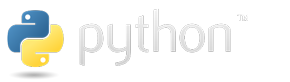
\includegraphics[keepaspectratio]{index_files/mediabag/python-logo.png}}

}

\caption{Python}

\end{figure}%

Para instalar Python en tu computadora, sigue los siguientes pasos:

\begin{enumerate}
\def\labelenumi{\arabic{enumi}.}
\tightlist
\item
  Ve al sitio web oficial de Python en \url{https://www.python.org/}.
\end{enumerate}

\begin{figure}[H]

{\centering \pandocbounded{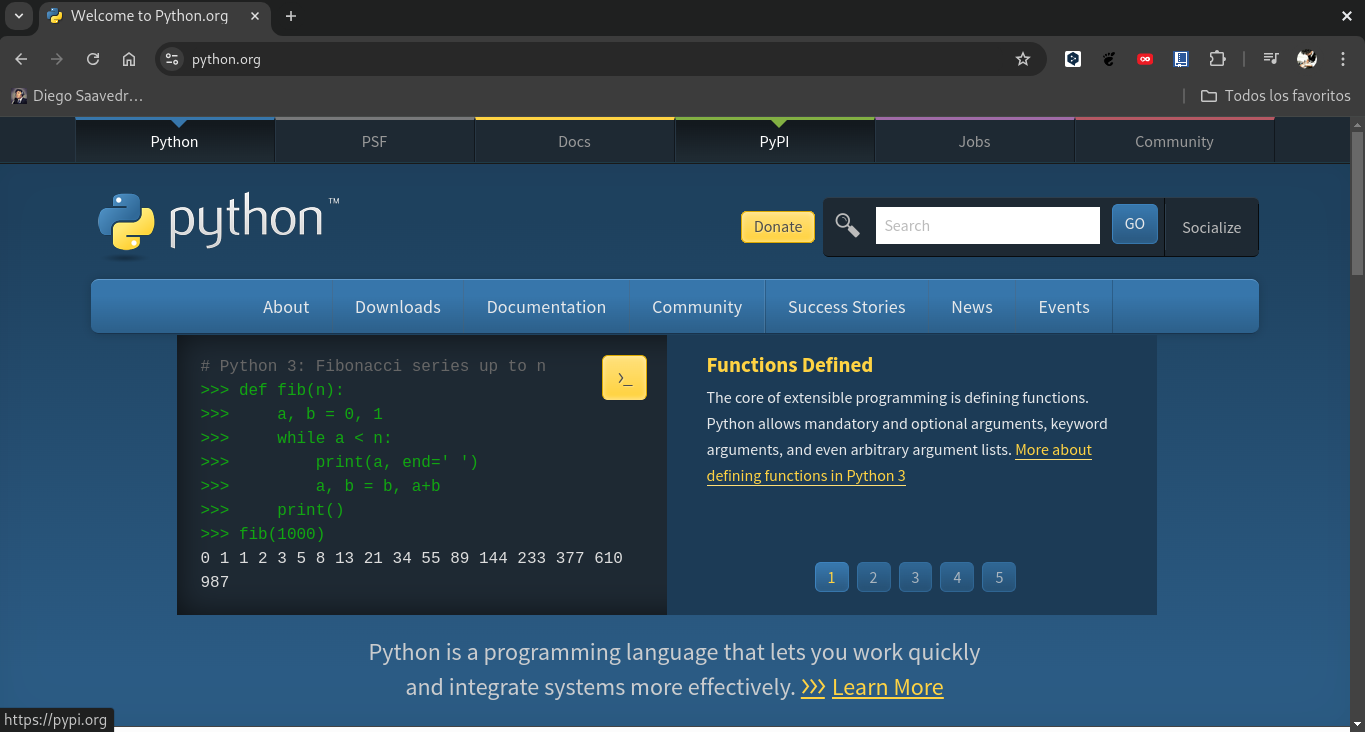
\includegraphics[keepaspectratio]{unidades/unidad1/images/python.org.png}}

}

\caption{Python}

\end{figure}%

\begin{enumerate}
\def\labelenumi{\arabic{enumi}.}
\setcounter{enumi}{1}
\tightlist
\item
  Haz clic en el botón de descarga de Python.
\end{enumerate}

\begin{figure}[H]

{\centering \pandocbounded{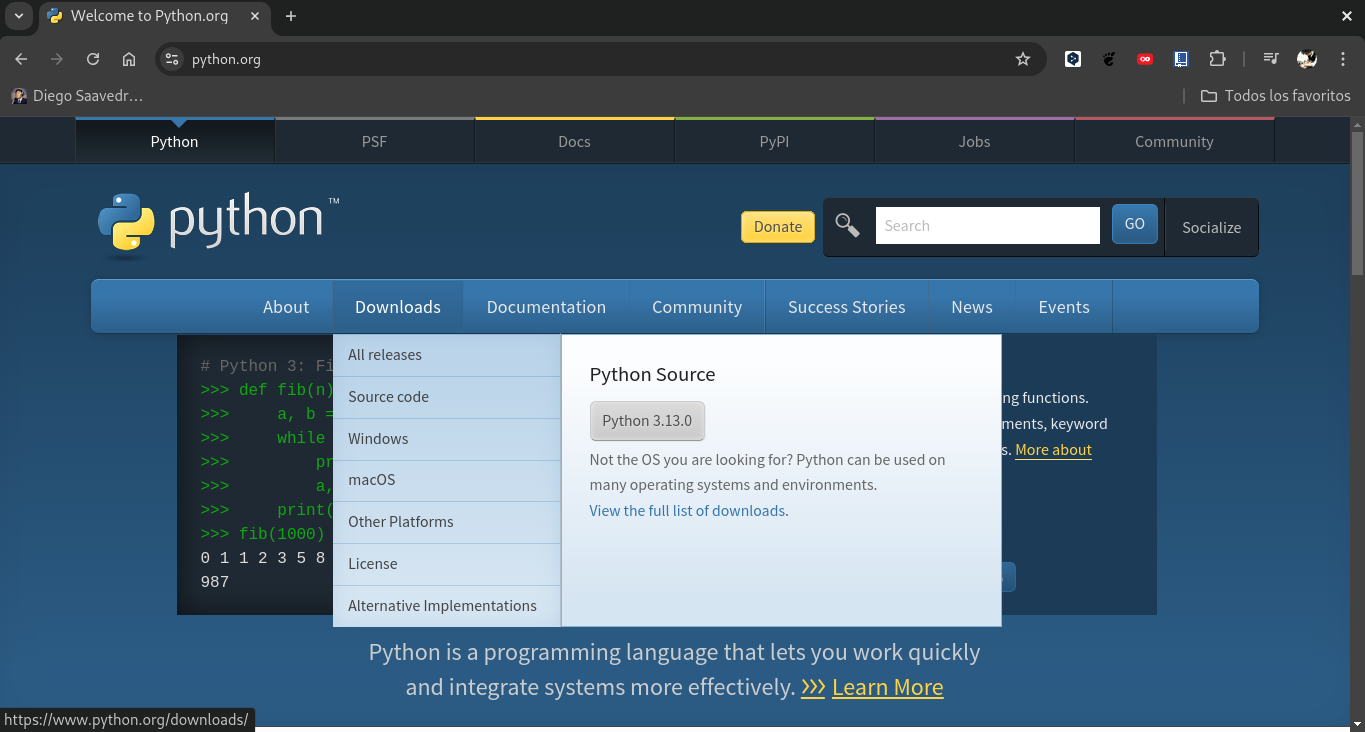
\includegraphics[keepaspectratio]{unidades/unidad1/images/download.png}}

}

\caption{Python}

\end{figure}%

\begin{enumerate}
\def\labelenumi{\arabic{enumi}.}
\setcounter{enumi}{2}
\item
  Selecciona la versión de Python que deseas instalar (recomendamos la
  versión más reciente).
\item
  Descarga el instalador de Python para tu sistema operativo (Windows,
  macOS o Linux).
\end{enumerate}

\begin{figure}[H]

{\centering \pandocbounded{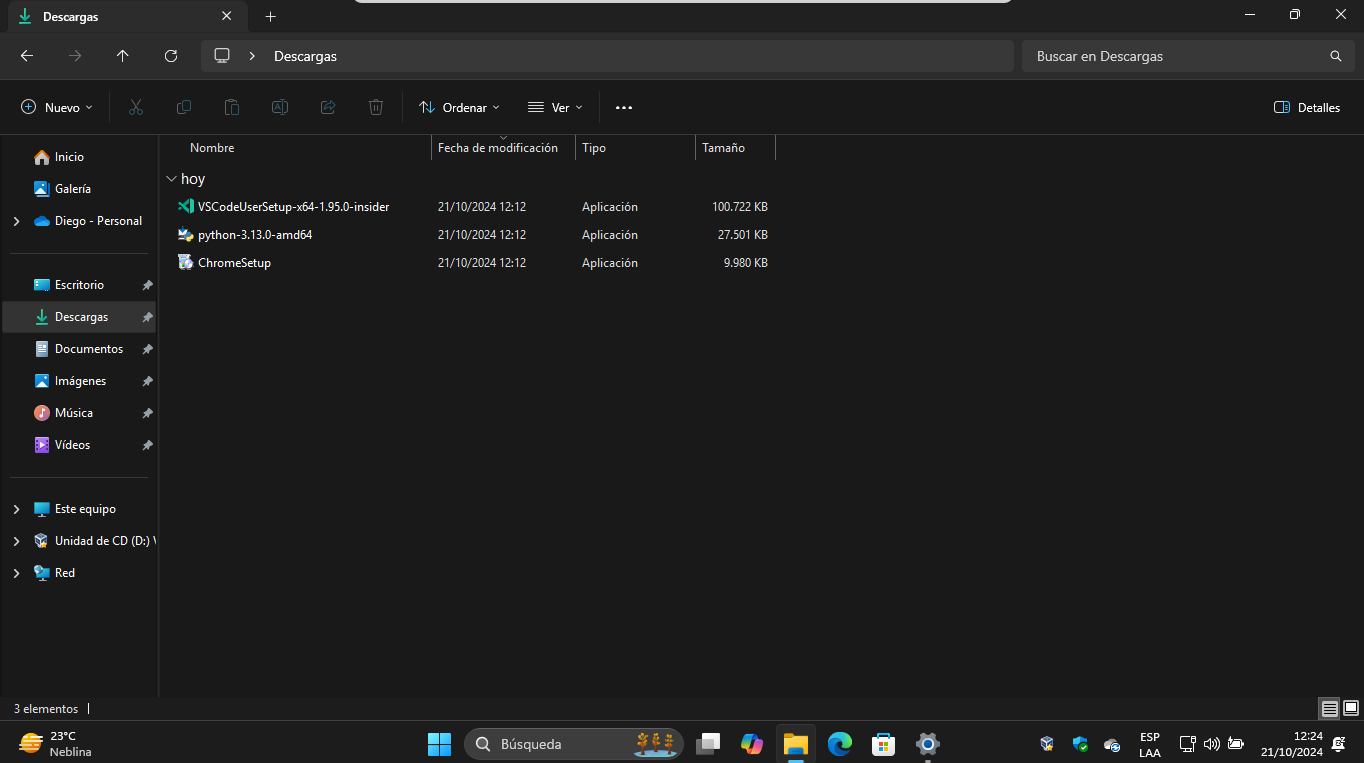
\includegraphics[keepaspectratio]{unidades/unidad1/images/instalador_python.png}}

}

\caption{Python}

\end{figure}%

\begin{enumerate}
\def\labelenumi{\arabic{enumi}.}
\setcounter{enumi}{4}
\tightlist
\item
  Ejecuta el instalador de Python y sigue las instrucciones en pantalla
  para completar la instalación.
\end{enumerate}

\begin{figure}[H]

{\centering \pandocbounded{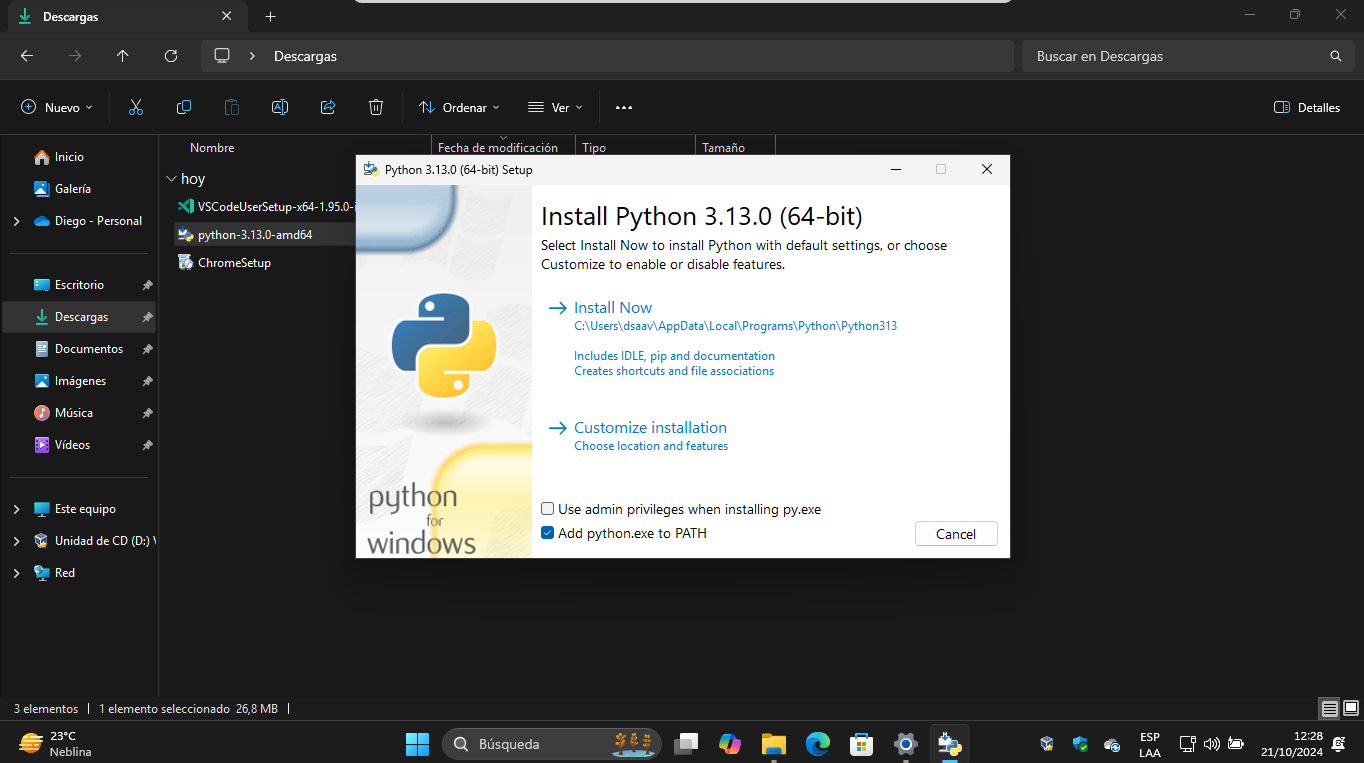
\includegraphics[keepaspectratio]{unidades/unidad1/images/add_to_path.png}}

}

\caption{Python}

\end{figure}%

Una vez que hayas instalado Python en tu computadora, puedes verificar
que la instalación se haya realizado correctamente abriendo una terminal
y ejecutando el siguiente comando:

\begin{figure}[H]

{\centering \pandocbounded{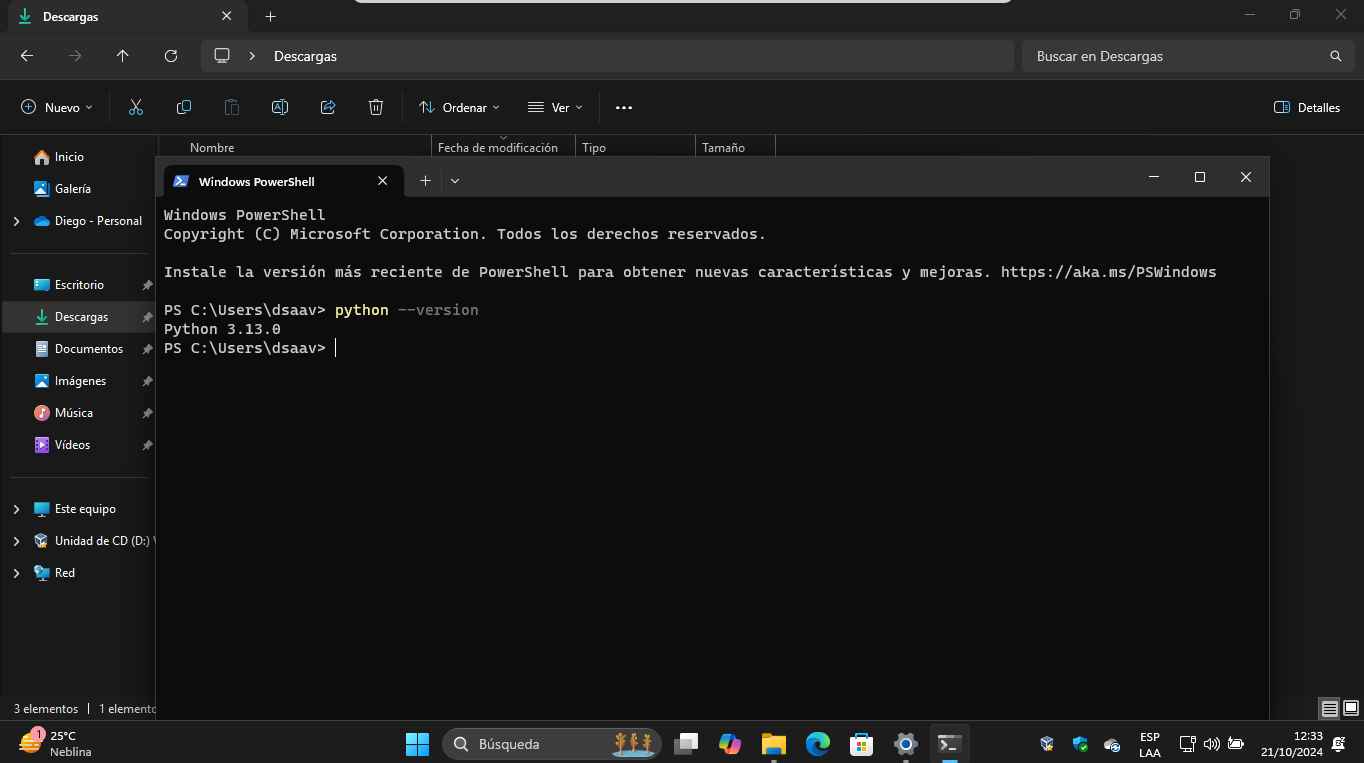
\includegraphics[keepaspectratio]{unidades/unidad1/images/python_version.png}}

}

\caption{Python}

\end{figure}%

\begin{Shaded}
\begin{Highlighting}[]
\ExtensionTok{python} \AttributeTok{{-}{-}version}
\end{Highlighting}
\end{Shaded}

Si la instalación se realizó correctamente, verás la versión de Python
instalada en tu computadora.

\section{Uso de REPL, PEP 8 y Zen de
Python}\label{uso-de-repl-pep-8-y-zen-de-python}

En esta sección, aprenderemos acerca de REPL, PEP 8 y Zen de Python.

\subsection{REPL}\label{repl}

REPL (Read-Eval-Print Loop) es un entorno interactivo que permite
escribir y ejecutar código de Python de manera interactiva. Es una
excelente herramienta para probar y experimentar con el lenguaje de
programación.

Para abrir el REPL de Python, abre una terminal y ejecuta el siguiente
comando:

\begin{Shaded}
\begin{Highlighting}[]
\ExtensionTok{python}
\end{Highlighting}
\end{Shaded}

Una vez que hayas abierto el REPL de Python, puedes escribir y ejecutar
código de Python de manera interactiva. Por ejemplo, puedes escribir una
expresión matemática y ver el resultado:

\begin{Shaded}
\begin{Highlighting}[]
\OperatorTok{\textgreater{}\textgreater{}\textgreater{}} \DecValTok{2} \OperatorTok{+} \DecValTok{2}
\OperatorTok{\textgreater{}\textgreater{}\textgreater{}} \DecValTok{4}
\OperatorTok{\textgreater{}\textgreater{}\textgreater{}} \DecValTok{3} \OperatorTok{*} \DecValTok{4}
\OperatorTok{\textgreater{}\textgreater{}\textgreater{}} \DecValTok{12}
\OperatorTok{\textgreater{}\textgreater{}\textgreater{}} \DecValTok{10} \OperatorTok{/} \DecValTok{2}
\OperatorTok{\textgreater{}\textgreater{}\textgreater{}} \FloatTok{5.0}
\OperatorTok{\textgreater{}\textgreater{}\textgreater{}} \DecValTok{2} \OperatorTok{**} \DecValTok{3}
\OperatorTok{\textgreater{}\textgreater{}\textgreater{}} \DecValTok{8}
\OperatorTok{\textgreater{}\textgreater{}\textgreater{}} \StringTok{"Hola, Mundo!"}
\OperatorTok{\textgreater{}\textgreater{}\textgreater{}} \StringTok{\textquotesingle{}Hola, Mundo!\textquotesingle{}}
\OperatorTok{\textgreater{}\textgreater{}\textgreater{}} \StringTok{"Hola, "} \OperatorTok{+} \StringTok{"Mundo!"}
\OperatorTok{\textgreater{}\textgreater{}\textgreater{}} \StringTok{\textquotesingle{}Hola, \textquotesingle{}} \OperatorTok{*} \DecValTok{3}
\OperatorTok{\textgreater{}\textgreater{}\textgreater{}} \StringTok{\textquotesingle{}Hola, Hola, Hola, \textquotesingle{}}
\OperatorTok{\textgreater{}\textgreater{}\textgreater{}} \BuiltInTok{print}\NormalTok{(}\StringTok{"Hola, Mundo!"}\NormalTok{)}
\OperatorTok{\textgreater{}\textgreater{}\textgreater{}}\NormalTok{ Hola, Mundo}\OperatorTok{!}
\end{Highlighting}
\end{Shaded}

\chapter{Pep 8}\label{pep-8}

PEP 8 (Python Enhancement Proposal 8) es una guía de estilo para
escribir código de Python de manera clara y legible. Es una excelente
referencia para seguir buenas prácticas de codificación y mantener un
código limpio y ordenado.

Algunas recomendaciones de PEP 8 son:

\begin{itemize}
\item
  Utiliza sangrías de 4 espacios para indentar el código.
\item
  Utiliza líneas en blanco para separar funciones y clases.
\item
  Utiliza nombres descriptivos para las variables y funciones.
\item
  Utiliza comentarios para explicar el código y hacerlo más legible.
\item
  Utiliza espacios alrededor de los operadores y después de las comas.
\item
  Utiliza comillas simples o dobles de manera consistente para las
  cadenas de texto.
\item
  Utiliza la función \textbf{print()} para imprimir en la consola.
\end{itemize}

\chapter{Zen de python.}\label{zen-de-python.}

El Zen de Python es una colección de 19 aforismos que resumen los
principios de diseño y filosofía de Python. Fueron escritos por Tim
Peters, uno de los desarrolladores originales de Python, y se pueden ver
en cualquier instalación de Python utilizando el siguiente comando:

\begin{Shaded}
\begin{Highlighting}[]
\ExtensionTok{import}\NormalTok{ this}
\end{Highlighting}
\end{Shaded}

Algunos de los aforismos más conocidos del Zen de Python son:

\begin{itemize}
\item
  Hermoso es mejor que feo.
\item
  Explícito es mejor que implícito.
\item
  Simple es mejor que complejo.
\item
  Complejo es mejor que complicado.
\item
  La legibilidad cuenta.
\item
  Los casos especiales no son lo suficientemente especiales como para
  romper las reglas.
\item
  Si la implementación es difícil de explicar, es una mala idea.
\item
  Si la implementación es fácil de explicar, puede que sea una buena
  idea.
\item
  Los errores nunca deberían pasar en silencio.
\item
  A menos que sean silenciados.
\item
  En la cara de la ambigüedad, rechaza la tentación de adivinar.
\item
  Debería haber una, y preferiblemente solo una, manera obvia de
  hacerlo.
\item
  Aunque esa manera puede no ser obvia al principio a menos que seas
  holandés.
\end{itemize}

En el ejemplo anterior, hemos utilizado el REPL de Python para ejecutar
expresiones matemáticas y cadenas de texto. Es una excelente manera de
probar y experimentar con el lenguaje de programación.

\section{Entornos de Desarrollo}\label{entornos-de-desarrollo}

Un entorno de desarrollo es un conjunto de herramientas que nos permiten
escribir, depurar y ejecutar código de manera eficiente. Es fundamental
para desarrollar programas y sistemas de manera efectiva.

Existen varios entornos de desarrollo que podemos utilizar para
programar en Python. Algunos de los más populares son:

\begin{itemize}
\tightlist
\item
  \textbf{IDLE}: Es el entorno de desarrollo integrado (IDE) oficial de
  Python. Viene incluido con la instalación de Python y es una excelente
  opción para programar en Python.
\end{itemize}

\begin{figure}[H]

{\centering \pandocbounded{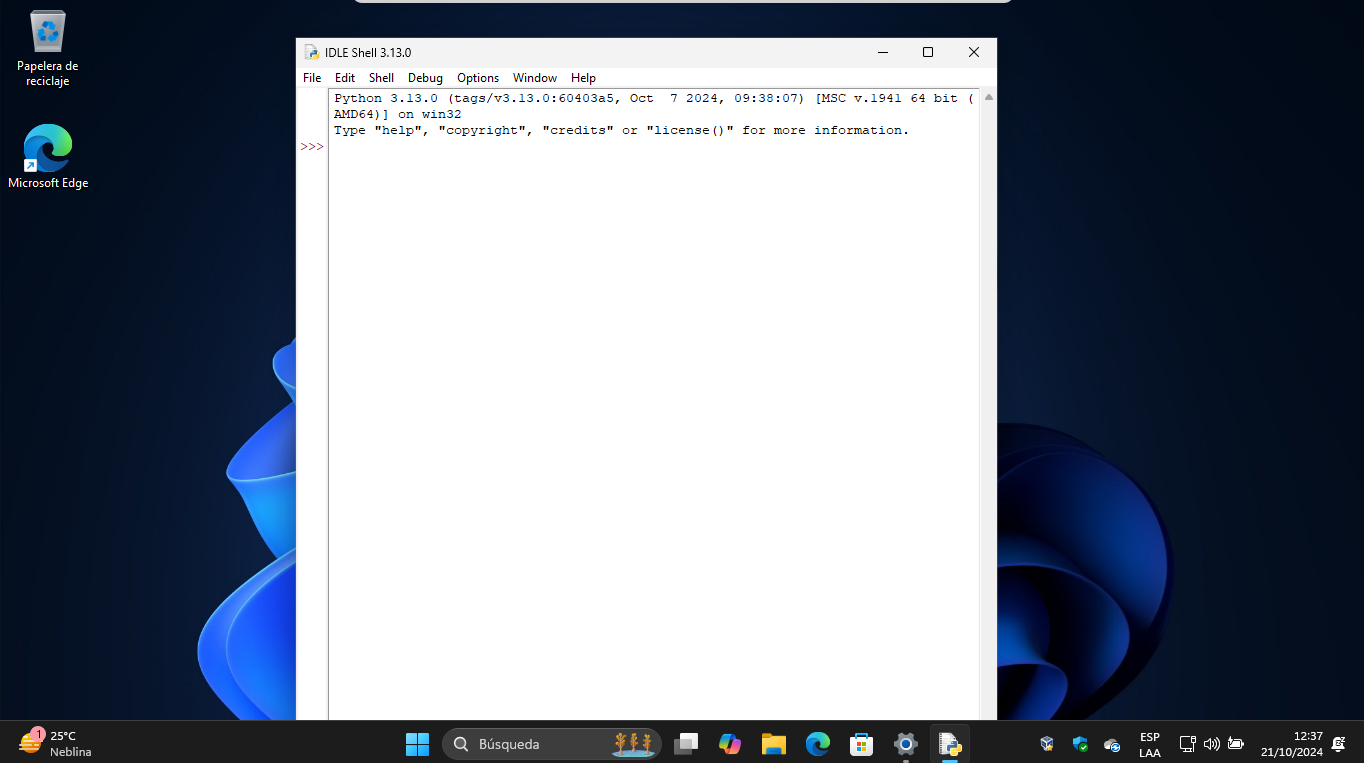
\includegraphics[keepaspectratio]{unidades/unidad1/images/idle_python.png}}

}

\caption{IDLE}

\end{figure}%

\begin{itemize}
\tightlist
\item
  \textbf{PyCharm}: Es un IDE de Python desarrollado por JetBrains. Es
  una excelente opción para programar en Python, ya que ofrece muchas
  características y herramientas útiles.
\end{itemize}

\begin{figure}[H]

{\centering \pandocbounded{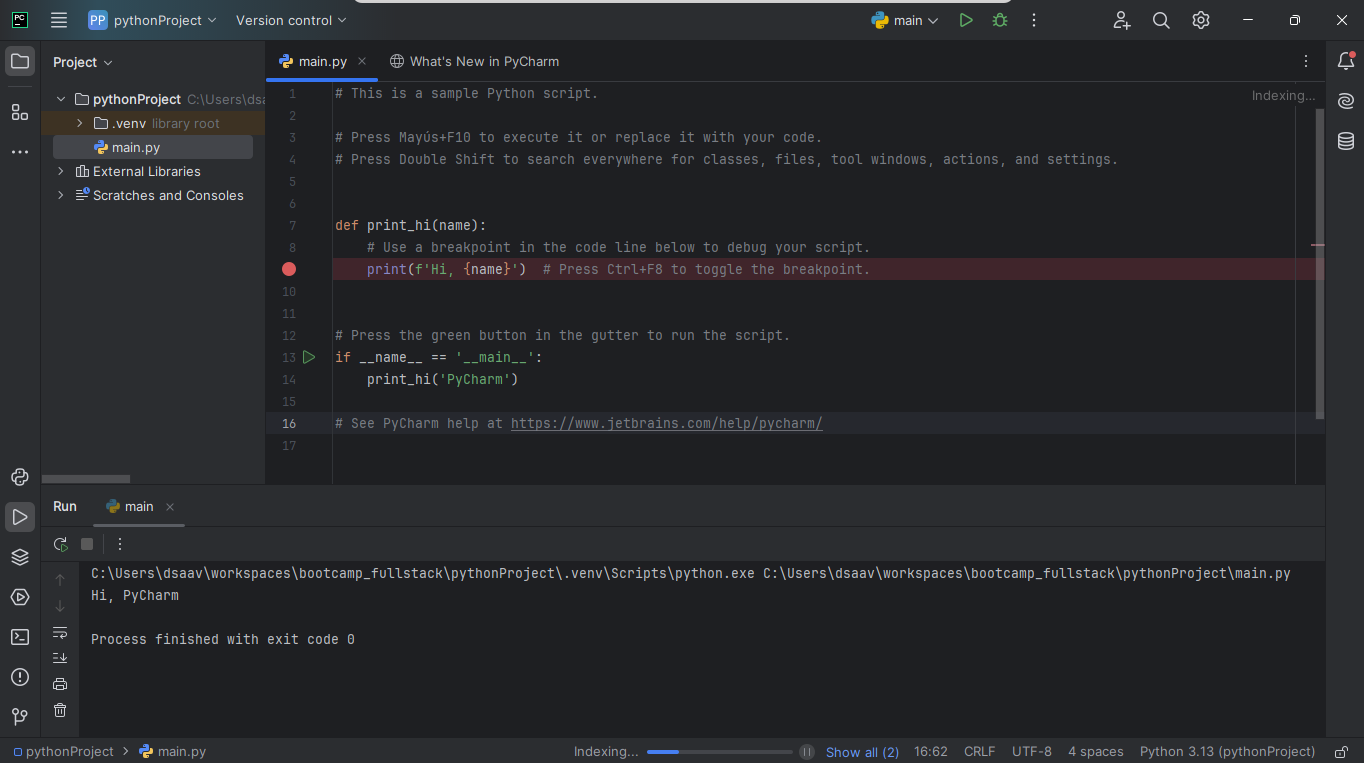
\includegraphics[keepaspectratio]{unidades/unidad1/images/pycharm.png}}

}

\caption{PyCharm}

\end{figure}%

\begin{itemize}
\tightlist
\item
  \textbf{Visual Studio Code}: Es un editor de código desarrollado por
  Microsoft. Es una excelente opción para programar en Python, ya que
  ofrece muchas extensiones y herramientas útiles.
\end{itemize}

\begin{figure}[H]

{\centering \pandocbounded{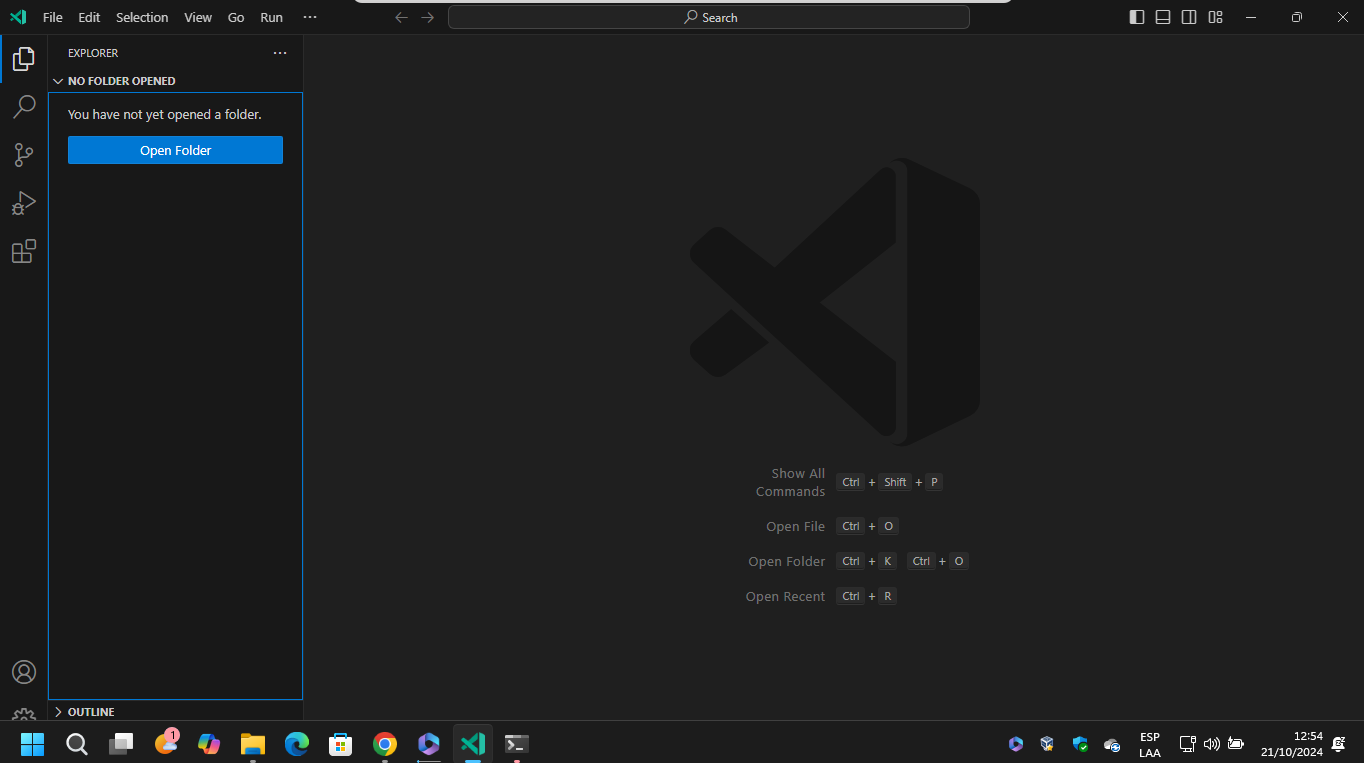
\includegraphics[keepaspectratio]{unidades/unidad1/images/vscode.png}}

}

\caption{Visual Studio Code}

\end{figure}%

\begin{itemize}
\tightlist
\item
  \textbf{Jupyter Notebook}: Es una aplicación web que nos permite crear
  y compartir documentos interactivos que contienen código de Python,
  visualizaciones y texto explicativo.
\end{itemize}

\begin{figure}[H]

{\centering \pandocbounded{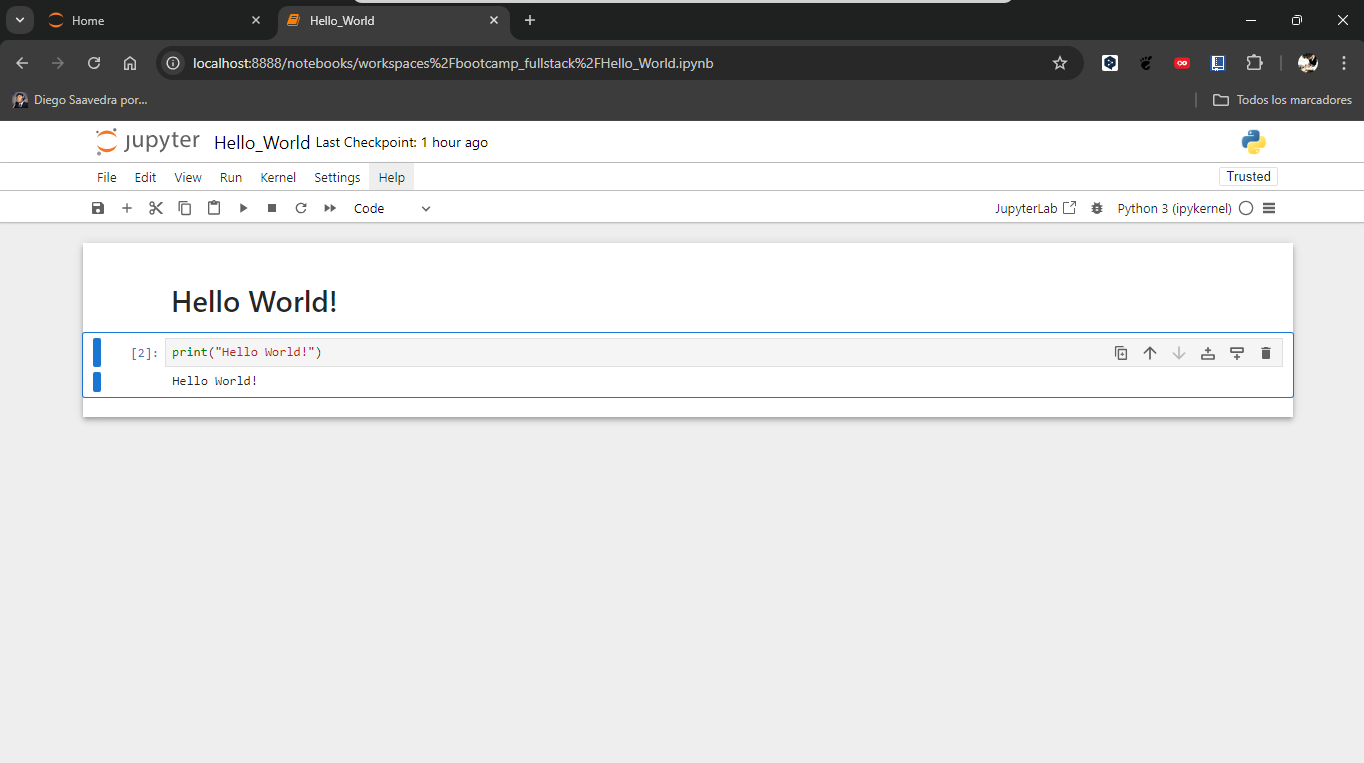
\includegraphics[keepaspectratio]{unidades/unidad1/images/jupyter_notebook.png}}

}

\caption{Jupyter Notebook}

\end{figure}%

En este bootcam utilizaremos \textbf{Visual Studio Code} como editor de
código para programar en Python. Sin embargo, te recomiendo que explores
otros entornos de desarrollo y elijas el que mejor se adapte a tus
necesidades y preferencias.

\section{5 Consejos para mejorar la lógica de
programación.}\label{consejos-para-mejorar-la-luxf3gica-de-programaciuxf3n.}

\begin{enumerate}
\def\labelenumi{\arabic{enumi}.}
\item
  \textbf{Practica regularmente}: La práctica es fundamental para
  mejorar la lógica de programación. Dedica tiempo a resolver problemas
  de programación y desafíos lógicos de manera regular.
\item
  \textbf{Descompón el problema}: Divide los problemas complejos en
  problemas más pequeños y manejables. Esto te ayudará a abordar el
  problema de manera más efectiva y eficiente.
\item
  \textbf{Utiliza pseudocódigo}: Antes de escribir código, utiliza
  pseudocódigo para planificar y diseñar tu solución. Esto te ayudará a
  visualizar el problema y encontrar una solución más clara.
\item
  \textbf{Comenta tu código}: Utiliza comentarios para explicar tu
  código y hacerlo más legible. Esto te ayudará a entender tu código y a
  identificar posibles errores.
\item
  \textbf{Colabora con otros}: Trabaja en equipo con otros programadores
  para resolver problemas de programación. La colaboración te permitirá
  aprender de otros y mejorar tus habilidades de programación.
\end{enumerate}

¡Espero que estos consejos te sean útiles para mejorar tu lógica de
programación!

\section{Conclusiones}\label{conclusiones}

En este módulo hemos aprendido acerca de la introducción general a la
programación, la instalación de Python, el uso de REPL, PEP 8 y Zen de
Python, y los entornos de desarrollo que podemos utilizar para programar
en Python.

\chapter{Introducción a la Programación con
Python}\label{introducciuxf3n-a-la-programaciuxf3n-con-python}

\begin{figure}[H]

{\centering \pandocbounded{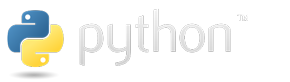
\includegraphics[keepaspectratio]{index_files/mediabag/python-logo.png}}

}

\caption{Python}

\end{figure}%

\section{¿Qué es la programación?}\label{quuxe9-es-la-programaciuxf3n}

La programación es el proceso de diseñar e implementar un programa de
computadora. Un programa es un conjunto de instrucciones que le dice a
la computadora qué hacer. Estas instrucciones pueden ser escritas en
diferentes lenguajes de programación, como Python, Java, C++, entre
otros.

\section{¿Qué es Python?}\label{quuxe9-es-python}

Python es un lenguaje de programación de alto nivel, interpretado y
orientado a objetos. Fue creado por Guido van Rossum en 1991 y es uno de
los lenguajes de programación más populares en la actualidad. Python es
conocido por su sintaxis simple y legible, lo que lo hace ideal para
principiantes en programación.

\section{¿Por qué aprender Python?}\label{por-quuxe9-aprender-python}

Python es un lenguaje de programación versátil que se puede utilizar
para una amplia variedad de aplicaciones, como desarrollo web, análisis
de datos, inteligencia artificial, entre otros. Además, Python es fácil
de aprender y de usar, lo que lo convierte en una excelente opción para
aquellos que quieren iniciarse en la programación.

\section{¿Qué aprenderemos en este
bootcamp?}\label{quuxe9-aprenderemos-en-este-bootcamp}

En este bootcamp aprenderemos los conceptos básicos de programación con
Python, incluyendo variables, tipos de datos, operadores, estructuras de
control, funciones, entre otros. Al final del bootcamp, tendrás los
conocimientos necesarios para crear tus propios programas en Python y
continuar tu aprendizaje en programación.

¡Vamos a empezar!

\section{Identación en Python}\label{identaciuxf3n-en-python}

Python utiliza la identación para definir bloques de código. La
identación es el espacio en blanco al principio de una línea de código y
se utiliza para indicar que una línea de código pertenece a un bloque de
código. Por ejemplo, en el siguiente código, la línea
\textbf{print(``Hola, mundo!'')} está identada con cuatro espacios, lo
que indica que pertenece al bloque de código del \textbf{if}.

\begin{Shaded}
\begin{Highlighting}[]
\ControlFlowTok{if} \VariableTok{True}\NormalTok{:}
    \BuiltInTok{print}\NormalTok{(}\StringTok{"Hola, mundo!"}\NormalTok{)}
\end{Highlighting}
\end{Shaded}

En el código anterior, la línea \textbf{print(``Hola, mundo!'')} se
ejecutará si la condición del \textbf{if} es verdadera. Si la línea no
estuviera identada, no se ejecutaría dentro del bloque de código del
\textbf{if}.

\section{Comentarios en python}\label{comentarios-en-python}

Los comentarios son líneas de texto que se utilizan para explicar el
código y hacerlo más legible. En Python, los comentarios se crean
utilizando el símbolo \textbf{\#}. Todo lo que sigue al símbolo
\textbf{\#} en una línea se considera un comentario y no se ejecuta como
código.

\begin{Shaded}
\begin{Highlighting}[]
\CommentTok{\# Este es un comentarios}
\BuiltInTok{print}\NormalTok{(}\StringTok{"Hola, mundo!"}\NormalTok{) }\CommentTok{\# Este es otro comentarios}
\end{Highlighting}
\end{Shaded}

En el código anterior, la línea \textbf{print(``Hola, mundo!'')} se
ejecutará, pero los comentarios no se ejecutarán.

\section{Variables y Variables
Múltiples}\label{variables-y-variables-muxfaltiples}

Una variable es un contenedor que se utiliza para almacenar datos en un
programa. En Python, una variable se crea asignando un valor a un nombre
de variable. Por ejemplo, en el siguiente código, la variable
\textbf{nombre} se crea y se le asigna el valor \textbf{``Juan''}.

\begin{Shaded}
\begin{Highlighting}[]
\NormalTok{nombre }\OperatorTok{=} \StringTok{"Juan"}
\BuiltInTok{print}\NormalTok{(nombre)}
\end{Highlighting}
\end{Shaded}

En el código anterior, la variable \textbf{nombre} se imprime en la
consola y se muestra el valor \textbf{``Juan''}.

En Python, también se pueden crear múltiples variables en una sola
línea. Por ejemplo, en el siguiente código, se crean tres variables
\textbf{a}, \textbf{b} y \textbf{c} y se les asignan los valores
\textbf{1}, \textbf{2} y \textbf{3} respectivamente.

\begin{Shaded}
\begin{Highlighting}[]
\NormalTok{a, b, c }\OperatorTok{=} \DecValTok{1}\NormalTok{, }\DecValTok{2}\NormalTok{, }\DecValTok{3}
\BuiltInTok{print}\NormalTok{(a, b, c)}
\end{Highlighting}
\end{Shaded}

En el código anterior, las variables \textbf{a}, \textbf{b} y \textbf{c}
se imprimen en la consola y se muestran los valores \textbf{1},
\textbf{2} y \textbf{3} respectivamente.

\section{Concatenación de Cadenas}\label{concatenaciuxf3n-de-cadenas}

La concatenación de cadenas es la unión de dos o más cadenas en una sola
cadena. En Python, se puede concatenar cadenas utilizando el operador
\textbf{+}. Por ejemplo, en el siguiente código, se concatenan las
cadenas \textbf{``Hola''} y \textbf{``mundo''} en una sola cadena.

\begin{Shaded}
\begin{Highlighting}[]
\NormalTok{saludo }\OperatorTok{=} \StringTok{"Hola"} \OperatorTok{+} \StringTok{"mundo"}
\BuiltInTok{print}\NormalTok{(saludo)}
\end{Highlighting}
\end{Shaded}

En el código anterior, la variable \textbf{saludo} se imprime en la
consola y se muestra la cadena \textbf{``Hola mundo''}.

Algunos ejemplos adicionales de concatenación de cadenas son:

\begin{Shaded}
\begin{Highlighting}[]
\NormalTok{nombre }\OperatorTok{=} \StringTok{"Juan"}
\NormalTok{apellido }\OperatorTok{=} \StringTok{"Pérez"}
\NormalTok{nombre\_completo }\OperatorTok{=}\NormalTok{ nombre }\OperatorTok{+} \StringTok{" "} \OperatorTok{+}\NormalTok{ apellido}
\BuiltInTok{print}\NormalTok{(nombre\_completo)}
\end{Highlighting}
\end{Shaded}

En el código anterior, la variable \textbf{nombre\_completo} se imprime
en la consola y se muestra la cadena \textbf{``Juan Pérez''}.

\begin{Shaded}
\begin{Highlighting}[]
\NormalTok{edad }\OperatorTok{=} \DecValTok{30}
\NormalTok{mensaje }\OperatorTok{=} \StringTok{"Tengo "} \OperatorTok{+} \BuiltInTok{str}\NormalTok{(edad) }\OperatorTok{+} \StringTok{" años"}
\BuiltInTok{print}\NormalTok{(mensaje)}
\end{Highlighting}
\end{Shaded}

En el código anterior, la variable \textbf{mensaje} se imprime en la
consola y se muestra la cadena \textbf{``Tengo 30 años''}.

\chapter{Actividad}\label{actividad}

\section{instrucciones}\label{instrucciones}

\begin{enumerate}
\def\labelenumi{\arabic{enumi}.}
\item
  Crea una variable llamada \textbf{nombre} y asígnale tu nombre.
\item
  Crea una variable llamada \textbf{edad} y asígnale tu edad.
\item
  Crea una variable llamada \textbf{ciudad} y asígnale tu ciudad de
  origen.
\item
  Imprime en la consola un mensaje que contenga tu nombre, edad y ciudad
  de origen utilizando la concatenación de cadenas.
\item
  Crea una variable llamada \textbf{mensaje} y asígnale el siguiente
  mensaje: ``Hola, mi nombre es {[}nombre{]}, tengo {[}edad{]} años y
  soy de {[}ciudad{]}.''
\item
  Imprime en la consola el mensaje utilizando la variable
  \textbf{mensaje}.
\end{enumerate}

🔍 Pistas

\begin{itemize}
\tightlist
\item
  Para concatenar cadenas en Python, utiliza el operador \textbf{+}.

  \begin{itemize}
  \tightlist
  \item
    Para convertir un número entero en una cadena, utiliza la función
    \textbf{str()}.
  \end{itemize}
\end{itemize}

\chapter{Conclusión}\label{conclusiuxf3n-1}

En este módulo, aprendimos los conceptos básicos de programación con
Python, incluyendo variables, identación, comentarios y concatenación de
cadenas. Estos conceptos son fundamentales para comprender y escribir
programas en Python. En los módulos siguientes, profundizaremos en otros
aspectos de la programación con Python, como tipos de datos, operadores,
estructuras de control, funciones, entre otros. ¡Sigue adelante!

\chapter{Tipos de Datos}\label{tipos-de-datos}

\begin{figure}[H]

{\centering \pandocbounded{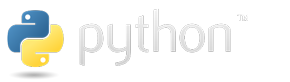
\includegraphics[keepaspectratio]{index_files/mediabag/python-logo.png}}

}

\caption{Python}

\end{figure}%

Los tipos de Datos en Python son la forma en que Python clasifica y
almacena los datos. Los tipos de datos más comunes en Python son:

\begin{itemize}
\tightlist
\item
  Números
\item
  Cadenas
\item
  Listas
\item
  Tuplas
\item
  Diccionarios
\item
  Booleanos
\item
  Rango
\end{itemize}

En esta actividad, aprenderás sobre los diferentes tipos de datos en
Python y cómo se utilizan.

\section{String y Números.}\label{string-y-nuxfameros.}

Los String y los Números son dos de los tipos de datos más comunes en
Python. Los String son secuencias de caracteres, como letras, números y
símbolos, que se utilizan para representar texto. Los Números, por otro
lado, son valores numéricos, como enteros y decimales, que se utilizan
para realizar cálculos matemáticos.

\subsection{String}\label{string}

Los String en Python se crean utilizando comillas simples \textbf{' '} o
comillas dobles \textbf{'' ``}. Por ejemplo:

\begin{Shaded}
\begin{Highlighting}[]
\NormalTok{nombre }\OperatorTok{=} \StringTok{"Juan"}
\NormalTok{apellido }\OperatorTok{=} \StringTok{\textquotesingle{}Pérez\textquotesingle{}}
\end{Highlighting}
\end{Shaded}

En el código anterior, se crean dos variables, \textbf{nombre} y
\textbf{apellido}, que contienen los String \textbf{``Juan''} y
\textbf{``Pérez''} respectivamente.

\subsection{Números}\label{nuxfameros}

Los Números en Python pueden ser enteros o decimales. Los enteros son
números enteros, como \textbf{1}, \textbf{2}, \textbf{3}, mientras que
los decimales son números con decimales, como \textbf{1.5},
\textbf{2.75}, \textbf{3.14}. Por ejemplo:

\begin{Shaded}
\begin{Highlighting}[]
\NormalTok{entero }\OperatorTok{=} \DecValTok{10}
\NormalTok{decimal }\OperatorTok{=} \FloatTok{3.14}
\end{Highlighting}
\end{Shaded}

En el código anterior, se crean dos variables, \textbf{entero} y
\textbf{decimal}, que contienen los números \textbf{10} y \textbf{3.14}
respectivamente.

\section{Listas y Tuplas.}\label{listas-y-tuplas.}

Las listas y las tuplas son dos tipos de datos en Python que se utilizan
para almacenar colecciones de elementos. Las listas son colecciones
ordenadas y modificables de elementos, mientras que las tuplas son
colecciones ordenadas e inmutables de elementos.

\subsection{Listas}\label{listas}

Las listas en Python se crean utilizando corchetes \textbf{{[} {]}} y
pueden contener cualquier tipo de datos, como números, String, listas,
tuplas, diccionarios, etc. Por ejemplo:

\begin{Shaded}
\begin{Highlighting}[]
\NormalTok{numeros }\OperatorTok{=}\NormalTok{ [}\DecValTok{1}\NormalTok{, }\DecValTok{2}\NormalTok{, }\DecValTok{3}\NormalTok{, }\DecValTok{4}\NormalTok{, }\DecValTok{5}\NormalTok{]}
\NormalTok{nombres }\OperatorTok{=}\NormalTok{ [}\StringTok{"Juan"}\NormalTok{, }\StringTok{"María"}\NormalTok{, }\StringTok{"Pedro"}\NormalTok{]}
\end{Highlighting}
\end{Shaded}

En el código anterior, se crean dos listas, \textbf{numeros} y
\textbf{nombres}, que contienen los números \textbf{1}, \textbf{2},
\textbf{3}, \textbf{4}, \textbf{5} y los nombres \textbf{``Juan''},
\textbf{``María''}, \textbf{``Pedro''} respectivamente.

\subsection{Tuplas}\label{tuplas}

Las tuplas en Python se crean utilizando paréntesis \textbf{( )} y
pueden contener cualquier tipo de datos, como números, String, listas,
tuplas, diccionarios, etc. Por ejemplo:

\begin{Shaded}
\begin{Highlighting}[]
\NormalTok{coordenadas }\OperatorTok{=}\NormalTok{ (}\DecValTok{10}\NormalTok{, }\DecValTok{20}\NormalTok{)}
\NormalTok{colores }\OperatorTok{=}\NormalTok{ (}\StringTok{"rojo"}\NormalTok{, }\StringTok{"verde"}\NormalTok{, }\StringTok{"azul"}\NormalTok{)}
\end{Highlighting}
\end{Shaded}

En el código anterior, se crean dos tuplas, \textbf{coordenadas} y
\textbf{colores}, que contienen las coordenadas \textbf{(10, 20)} y los
colores \textbf{``rojo''}, \textbf{``verde''}, \textbf{``azul''}
respectivamente.

\section{Diccionarios y Booleanos.}\label{diccionarios-y-booleanos.}

Los diccionarios y los booleanos son dos tipos de datos en Python que se
utilizan para almacenar información y tomar decisiones.

\subsection{Diccionarios}\label{diccionarios}

Los diccionarios en Python se crean utilizando llaves \textbf{\{ \}} y
contienen pares de claves y valores. Por ejemplo:

\begin{Shaded}
\begin{Highlighting}[]
\NormalTok{persona }\OperatorTok{=}\NormalTok{ \{}\StringTok{"nombre"}\NormalTok{: }\StringTok{"Juan"}\NormalTok{, }\StringTok{"edad"}\NormalTok{: }\DecValTok{30}\NormalTok{, }\StringTok{"ciudad"}\NormalTok{: }\StringTok{"Bogotá"}\NormalTok{\}}
\end{Highlighting}
\end{Shaded}

En el código anterior, se crea un diccionario \textbf{persona} que
contiene las claves \textbf{``nombre''}, \textbf{``edad''} y
\textbf{``ciudad''} con los valores \textbf{``Juan''}, \textbf{30} y
\textbf{``Bogotá''} respectivamente.

\subsection{Booleanos}\label{booleanos}

Los booleanos en Python son valores lógicos que pueden ser \textbf{True}
o \textbf{False}. Se utilizan para tomar decisiones en un programa. Por
ejemplo:

\begin{Shaded}
\begin{Highlighting}[]
\NormalTok{es\_mayor\_de\_edad }\OperatorTok{=} \VariableTok{True}
\NormalTok{es\_estudiante }\OperatorTok{=} \VariableTok{False}
\end{Highlighting}
\end{Shaded}

En el código anterior, se crean dos variables booleanas,
\textbf{es\_mayor\_de\_edad} y \textbf{es\_estudiante}, que contienen
los valores \textbf{True} y \textbf{False} respectivamente.

\section{Range}\label{range}

El tipo de datos \textbf{range} en Python se utiliza para generar una
secuencia de números. Se crea utilizando la función \textbf{range()} y
puede contener hasta tres argumentos: \textbf{start}, \textbf{stop} y
\textbf{step}. Por ejemplo:

\begin{Shaded}
\begin{Highlighting}[]
\NormalTok{numeros }\OperatorTok{=} \BuiltInTok{range}\NormalTok{(}\DecValTok{1}\NormalTok{, }\DecValTok{10}\NormalTok{, }\DecValTok{2}\NormalTok{)}
\end{Highlighting}
\end{Shaded}

En el código anterior, se crea un objeto \textbf{range} llamado
\textbf{numeros} que contiene los números \textbf{1}, \textbf{3},
\textbf{5}, \textbf{7}, \textbf{9}.

\chapter{Actividad}\label{actividad-1}

\section{Instrucciones}\label{instrucciones-1}

\begin{enumerate}
\def\labelenumi{\arabic{enumi}.}
\item
  Crea una lista llamada \textbf{numeros} que contenga los números del
  \textbf{1} al \textbf{10}.
\item
  Crea una tupla llamada \textbf{colores} que contenga los colores
  \textbf{``rojo''}, \textbf{``verde''} y \textbf{``azul''}.
\item
  Crea un diccionario llamado \textbf{persona} que contenga las claves
  \textbf{``nombre''}, \textbf{``edad''} y \textbf{``ciudad''} con los
  valores \textbf{``Juan''}, \textbf{30} y \textbf{``Bogotá''}
  respectivamente.
\item
  Crea una variable booleana llamada \textbf{es\_mayor\_de\_edad} y
  asígnale el valor \textbf{True}.
\item
  Imprime en la consola las variables \textbf{numeros},
  \textbf{colores}, \textbf{persona} y \textbf{es\_mayor\_de\_edad}.
\item
  ¿Qué tipo de datos es la variable \textbf{numeros}? ¿Y la variable
  \textbf{colores}? ¿Y la variable \textbf{persona}? ¿Y la variable
  \textbf{es\_mayor\_de\_edad}?
\item
  ¿Qué tipo de datos es la variable \textbf{numeros{[}0{]}}? ¿Y la
  variable \textbf{colores{[}1{]}}? ¿Y la variable
  \textbf{persona{[}``nombre''{]}}? ¿Y la variable
  \textbf{es\_mayor\_de\_edad}?
\item
  ¿Qué tipo de datos es la variable \textbf{numeros{[}0:5{]}}? ¿Y la
  variable \textbf{colores{[}1:{]}}? ¿Y la variable
  \textbf{persona.keys()}? ¿Y la variable \textbf{es\_mayor\_de\_edad}?
\item
  ¿Qué tipo de datos es la variable \textbf{range(1, 10, 2)}? ¿Y la
  variable \textbf{range(10)}? ¿Y la variable \textbf{range(1, 10)}? ¿Y
  la variable \textbf{range(1, 10, 1)}?
\item
  ¿Qué tipo de datos es la variable \textbf{range(1, 10, 2){[}0{]}}? ¿Y
  la variable \textbf{range(10){[}0{]}}? ¿Y la variable \textbf{range(1,
  10){[}0{]}}? ¿Y la variable \textbf{range(1, 10, 1){[}0{]}}?
\end{enumerate}

Posibles soluciones

\begin{enumerate}
\def\labelenumi{\arabic{enumi}.}
\item
  La variable \textbf{numeros} es una lista.
\item
  La variable \textbf{colores} es una tupla.
\item
  La variable \textbf{persona} es un diccionario.
\item
  La variable \textbf{es\_mayor\_de\_edad} es un booleano.
\item
  La variable \textbf{numeros{[}0{]}} es un número.
\item
  La variable \textbf{colores{[}1{]}} es un String.
\item
  La variable \textbf{persona{[}``nombre''{]}} es un String.
\item
  La variable \textbf{numeros{[}0:5{]}} es una lista.
\item
  La variable \textbf{range(1, 10, 2)} es un objeto \textbf{range}.
\item
  La variable \textbf{range(1, 10, 2){[}0{]}} es un número.
\end{enumerate}

\chapter{Conclusiones}\label{conclusiones-1}

En esta actividad, aprendiste sobre los diferentes tipos de datos en
Python, como los String, los Números, las Listas, las Tuplas, los
Diccionarios, los Booleanos y el tipo de datos \textbf{range}.

También aprendiste cómo crear y utilizar estos tipos de datos en Python.
Ahora estás listo para utilizar estos conocimientos en tus propios
programas y proyectos.

¡Sigue practicando y mejorando tus habilidades de programación en
Python!

\chapter{Control de Flujo}\label{control-de-flujo}

\begin{figure}[H]

{\centering \pandocbounded{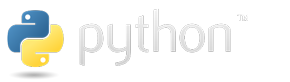
\includegraphics[keepaspectratio]{index_files/mediabag/python-logo.png}}

}

\caption{Python}

\end{figure}%

El control de flujo en Python se refiere a la forma en que se ejecutan
las instrucciones en un programa. Python proporciona varias estructuras
de control de flujo que permiten tomar decisiones, repetir tareas y
ejecutar instrucciones en función de ciertas condiciones.

La sintaxis de las estructuras de control de flujo en Python se basa en
la indentación, lo que significa que las instrucciones dentro de un
bloque de código deben estar indentadas con la misma cantidad de
espacios o tabulaciones. Esto hace que el código sea más legible y fácil
de entender.

En esta sección, aprenderemos sobre las siguientes estructuras de
control de flujo en Python:

\begin{itemize}
\tightlist
\item
  If y Condicionales
\item
  If, elif y else
\item
  And y Or
\item
  While loop
\item
  While, break y continue
\item
  For loop
\end{itemize}

\section{If y Condicionales}\label{if-y-condicionales}

Para entender el concepto de If y Condicionales en Python, primero
debemos comprender qué es una condición. Una condición es una expresión
que se evalúa como verdadera o falsa. En Python, las condiciones se
utilizan para tomar decisiones en un programa.

La estructura básica de un If en Python es la siguiente:

\begin{Shaded}
\begin{Highlighting}[]
\ControlFlowTok{if}\NormalTok{ condicion:}
    \CommentTok{\# Bloque de código si la condición es verdadera}
\end{Highlighting}
\end{Shaded}

En el código anterior, si la condición es verdadera, se ejecutará el
bloque de código dentro del If. Si la condición es falsa, el bloque de
código no se ejecutará.

Por ejemplo:

\begin{Shaded}
\begin{Highlighting}[]
\NormalTok{edad }\OperatorTok{=} \DecValTok{18}

\ControlFlowTok{if}\NormalTok{ edad }\OperatorTok{\textgreater{}=} \DecValTok{18}\NormalTok{:}
    \BuiltInTok{print}\NormalTok{(}\StringTok{"Eres mayor de edad"}\NormalTok{)}
\end{Highlighting}
\end{Shaded}

En el código anterior, si la variable \textbf{edad} es mayor o igual a
18, se imprimirá en la consola el mensaje ``Eres mayor de edad''.

\section{If, elif y else}\label{if-elif-y-else}

Además del If, Python también proporciona las palabras clave
\textbf{elif} y \textbf{else} para tomar decisiones más complejas en un
programa. La estructura básica de un If, elif y else en Python es la
siguiente:

\begin{Shaded}
\begin{Highlighting}[]
\ControlFlowTok{if}\NormalTok{ condicion1:}
    \CommentTok{\# Bloque de código si la condicion1 es verdadera}
\ControlFlowTok{elif}\NormalTok{ condicion2:}
    \CommentTok{\# Bloque de código si la condicion2 es verdadera}
\ControlFlowTok{else}\NormalTok{:}
    \CommentTok{\# Bloque de código si ninguna de las condiciones anteriores es verdadera}
\end{Highlighting}
\end{Shaded}

En el código anterior, si la \textbf{condicion1} es verdadera, se
ejecutará el bloque de código dentro del If. Si la \textbf{condicion1}
es falsa y la \textbf{condicion2} es verdadera, se ejecutará el bloque
de código dentro del \textbf{elif}. Si ninguna de las condiciones
anteriores es verdadera, se ejecutará el bloque de código dentro del
\textbf{else}.

Por ejemplo:

\begin{Shaded}
\begin{Highlighting}[]
\NormalTok{edad }\OperatorTok{=} \DecValTok{18}

\ControlFlowTok{if}\NormalTok{ edad }\OperatorTok{\textless{}} \DecValTok{18}\NormalTok{:}
    \BuiltInTok{print}\NormalTok{(}\StringTok{"Eres menor de edad"}\NormalTok{)}
\ControlFlowTok{elif}\NormalTok{ edad }\OperatorTok{==} \DecValTok{18}\NormalTok{:}
    \BuiltInTok{print}\NormalTok{(}\StringTok{"Tienes 18 años"}\NormalTok{)}
\ControlFlowTok{else}\NormalTok{:}
    \BuiltInTok{print}\NormalTok{(}\StringTok{"Eres mayor de edad"}\NormalTok{)}
\end{Highlighting}
\end{Shaded}

En el código anterior, si la variable \textbf{edad} es menor que 18, se
imprimirá en la consola el mensaje ``Eres menor de edad''. Si la
variable \textbf{edad} es igual a 18, se imprimirá en la consola el
mensaje ``Tienes 18 años''. Si ninguna de las condiciones anteriores es
verdadera, se imprimirá en la consola el mensaje ``Eres mayor de edad''.

\section{And y Or}\label{and-y-or}

Para entender el concepto de And y Or en Python, primero debemos
comprender cómo funcionan los operadores lógicos. Los operadores lógicos
se utilizan para combinar o modificar condiciones en una expresión
lógica.

En Python, los operadores lógicos más comunes son \textbf{and} y
\textbf{or}. El operador \textbf{and} devuelve \textbf{True} si ambas
condiciones son verdaderas. El operador \textbf{or} devuelve
\textbf{True} si al menos una de las condiciones es verdadera.

Por ejemplo:

\begin{Shaded}
\begin{Highlighting}[]
\NormalTok{edad }\OperatorTok{=} \DecValTok{18}

\ControlFlowTok{if}\NormalTok{ edad }\OperatorTok{\textgreater{}=} \DecValTok{18} \KeywordTok{and}\NormalTok{ edad }\OperatorTok{\textless{}=} \DecValTok{30}\NormalTok{:}
    \BuiltInTok{print}\NormalTok{(}\StringTok{"Tienes entre 18 y 30 años"}\NormalTok{)}
\end{Highlighting}
\end{Shaded}

En el código anterior, si la variable \textbf{edad} es mayor o igual a
18 y menor o igual a 30, se imprimirá en la consola el mensaje ``Tienes
entre 18 y 30 años''.

\section{While loop}\label{while-loop}

Para entender el concepto de While loop en Python, primero debemos
comprender qué es un bucle. Un bucle es una estructura de control que se
utiliza para repetir una secuencia de instrucciones varias veces. En
Python, el bucle \textbf{while} se utiliza para repetir un bloque de
código mientras una condición sea verdadera.

La estructura básica de un While loop en Python es la siguiente:

\begin{Shaded}
\begin{Highlighting}[]
\ControlFlowTok{while}\NormalTok{ condicion:}
    \CommentTok{\# Bloque de código que se repetirá mientras la condición sea verdadera}
\end{Highlighting}
\end{Shaded}

En el código anterior, si la condición es verdadera, se ejecutará el
bloque de código dentro del While loop. El bloque de código se repetirá
hasta que la condición sea falsa.

Por ejemplo:

\begin{Shaded}
\begin{Highlighting}[]
\NormalTok{contador }\OperatorTok{=} \DecValTok{0}

\ControlFlowTok{while}\NormalTok{ contador }\OperatorTok{\textless{}} \DecValTok{5}\NormalTok{:}
    \BuiltInTok{print}\NormalTok{(contador)}
\NormalTok{    contador }\OperatorTok{+=} \DecValTok{1}
\end{Highlighting}
\end{Shaded}

En el código anterior, se crea una variable \textbf{contador} con el
valor \textbf{0}. Luego, se ejecuta un While loop que imprime el valor
del \textbf{contador} y luego incrementa el \textbf{contador} en
\textbf{1} en cada iteración. El bucle se repetirá hasta que el
\textbf{contador} sea mayor o igual a \textbf{5}.

\section{While, break y continue}\label{while-break-y-continue}

Para entender el concepto de While, break y continue en Python, primero
debemos comprender cómo funcionan las palabras clave \textbf{break} y
\textbf{continue} en un bucle \textbf{while}.

La palabra clave \textbf{break} se utiliza para salir de un bucle
\textbf{while} antes de que la condición sea falsa. La palabra clave
\textbf{continue} se utiliza para saltar a la siguiente iteración del
bucle \textbf{while} sin ejecutar el resto del bloque de código.

Por ejemplo:

\begin{Shaded}
\begin{Highlighting}[]
\NormalTok{contador }\OperatorTok{=} \DecValTok{0}

\ControlFlowTok{while}\NormalTok{ contador }\OperatorTok{\textless{}} \DecValTok{5}\NormalTok{:}
    \ControlFlowTok{if}\NormalTok{ contador }\OperatorTok{==} \DecValTok{3}\NormalTok{:}
        \ControlFlowTok{break}
    \BuiltInTok{print}\NormalTok{(contador)}
\NormalTok{    contador }\OperatorTok{+=} \DecValTok{1}
\end{Highlighting}
\end{Shaded}

En el código anterior, se crea una variable \textbf{contador} con el
valor \textbf{0}. Luego, se ejecuta un While loop que imprime el valor
del \textbf{contador} y luego incrementa el \textbf{contador} en
\textbf{1} en cada iteración. Si el \textbf{contador} es igual a
\textbf{3}, se ejecuta la palabra clave \textbf{break} y se sale del
bucle.

\section{For loop}\label{for-loop}

Para entender el concepto de For loop en Python, primero debemos
comprender cómo funciona un bucle \textbf{for}. Un bucle \textbf{for} se
utiliza para iterar sobre una secuencia de elementos, como una lista,
una tupla, un diccionario, etc.

La estructura básica de un For loop en Python es la siguiente:

\begin{Shaded}
\begin{Highlighting}[]
\ControlFlowTok{for}\NormalTok{ elemento }\KeywordTok{in}\NormalTok{ secuencia:}
    \CommentTok{\# Bloque de código que se repetirá para cada elemento en la secuencia}
\end{Highlighting}
\end{Shaded}

En el código anterior, el bucle \textbf{for} recorre cada elemento en la
secuencia y ejecuta el bloque de código para cada elemento.

Por ejemplo:

\begin{Shaded}
\begin{Highlighting}[]
\NormalTok{numeros }\OperatorTok{=}\NormalTok{ [}\DecValTok{1}\NormalTok{, }\DecValTok{2}\NormalTok{, }\DecValTok{3}\NormalTok{, }\DecValTok{4}\NormalTok{, }\DecValTok{5}\NormalTok{]}

\ControlFlowTok{for}\NormalTok{ numero }\KeywordTok{in}\NormalTok{ numeros:}
    \BuiltInTok{print}\NormalTok{(numero)}
\end{Highlighting}
\end{Shaded}

En el código anterior, se crea una lista \textbf{numeros} con los
números del \textbf{1} al \textbf{5}. Luego, se ejecuta un For loop que
imprime cada número en la lista.

\chapter{Actividad}\label{actividad-2}

\section{instrucciones}\label{instrucciones-2}

\begin{enumerate}
\def\labelenumi{\arabic{enumi}.}
\item
  Crea una lista llamada \textbf{numeros} que contenga los números del
  \textbf{1} al \textbf{10}.
\item
  Crea una tupla llamada \textbf{colores} que contenga los colores
  \textbf{``rojo''}, \textbf{``verde''} y \textbf{``azul''}.
\item
  Crea un diccionario llamado \textbf{persona} que contenga las claves
  \textbf{``nombre''}, \textbf{``edad''} y \textbf{``ciudad''} con los
  valores \textbf{``Diego''}, \textbf{36} y \textbf{``Quito''}
  respectivamente.
\item
  Crea una variable booleana llamada \textbf{es\_mayor\_de\_edad} y
  asígnale el valor \textbf{True}.
\item
  Imprime en la consola las variables \textbf{numeros},
  \textbf{colores}, \textbf{persona} y \textbf{es\_mayor\_de\_edad}.
\item
  ¿Qué tipo de datos es la variable \textbf{numeros}? ¿Y la variable
  \textbf{colores}? ¿Y la variable \textbf{persona}? ¿Y la variable
  \textbf{es\_mayor\_de\_edad}?
\item
  ¿Qué tipo de datos es la variable \textbf{numeros{[}0{]}}? ¿Y la
  variable \textbf{colores{[}1{]}}? ¿Y la variable
  \textbf{persona{[}``nombre''{]}}? ¿Y la variable
  \textbf{es\_mayor\_de\_edad}?
\item
  ¿Qué tipo de datos es la variable \textbf{numeros{[}0:5{]}}? ¿Y la
  variable \textbf{colores{[}1:{]}}? ¿Y la variable
  \textbf{persona.keys()}? ¿Y la variable \textbf{es\_mayor\_de\_edad}?
\item
  ¿Qué tipo de datos es la variable \textbf{range(1, 10, 2)}? ¿Y la
  variable \textbf{range(10)}? ¿Y la variable \textbf{range(1, 10)}? ¿Y
  la variable \textbf{range(1, 10, 1)}?
\item
  ¿Qué tipo de datos es la variable \textbf{range(1, 10, 2){[}0{]}}? ¿Y
  la variable \textbf{range(10){[}0{]}}? ¿Y la variable \textbf{range(1,
  10){[}0{]}}? ¿Y la variable \textbf{range(1, 10, 1){[}0{]}}?
\end{enumerate}

Posibles soluciones

\begin{enumerate}
\def\labelenumi{\arabic{enumi}.}
\item
  La variable \textbf{numeros} es una lista.
\item
  La variable \textbf{colores} es una tupla.
\item
  La variable \textbf{persona} es un diccionario.
\item
  La variable \textbf{es\_mayor\_de\_edad} es un booleano.
\item
  La variable \textbf{numeros{[}0{]}} es un número.
\item
  La variable \textbf{colores{[}1{]}} es un String.
\item
  La variable \textbf{persona{[}``nombre''{]}} es un String.
\item
  La variable \textbf{numeros{[}0:5{]}} es una lista.
\item
  La variable \textbf{range(1, 10, 2)} es un objeto \textbf{range}.
\item
  La variable \textbf{range(1, 10, 2){[}0{]}} es un número.
\end{enumerate}

\chapter{Conclusiones}\label{conclusiones-2}

En esta sección, aprendimos sobre las estructuras de control de flujo en
Python, como If, elif, else, And, Or, While loop y For loop. Estas
estructuras nos permiten tomar decisiones, repetir tareas y ejecutar
instrucciones en función de ciertas condiciones en un programa. Es
importante comprender cómo funcionan estas estructuras para poder
escribir código más eficiente y legible en Python.

\chapter{Funciones y recursividad.}\label{funciones-y-recursividad.}

\begin{figure}[H]

{\centering \pandocbounded{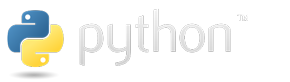
\includegraphics[keepaspectratio]{index_files/mediabag/python-logo.png}}

}

\caption{Python}

\end{figure}%

Las funciones son bloques de código reutilizables que realizan una tarea
específica. En Python, las funciones se definen utilizando la palabra
clave \textbf{def} seguida del nombre de la función y los parámetros
entre paréntesis. Por ejemplo:

\begin{Shaded}
\begin{Highlighting}[]
\KeywordTok{def}\NormalTok{ saludar():}
    \BuiltInTok{print}\NormalTok{(}\StringTok{"Hola, ¿cómo estás?"}\NormalTok{)}
\end{Highlighting}
\end{Shaded}

En el código anterior, se define una función llamada \textbf{saludar}
que imprime en la consola el mensaje ``Hola, ¿cómo estás?''. Para llamar
a una función en Python, simplemente se escribe el nombre de la función
seguido de paréntesis. Por ejemplo:

\begin{Shaded}
\begin{Highlighting}[]
\NormalTok{saludar()}
\end{Highlighting}
\end{Shaded}

En el código anterior, se llama a la función \textbf{saludar} y se
imprime en la consola el mensaje ``Hola, ¿cómo estás?''.

\section{Introducción a Funciones}\label{introducciuxf3n-a-funciones}

Para entender de mejor forma cómo funcionan las funciones en Python,
vamos a crear una función que reciba dos números como parámetros y
devuelva la suma de los mismos. Por ejemplo:

\begin{Shaded}
\begin{Highlighting}[]
\KeywordTok{def}\NormalTok{ sumar(a, b):}
    \ControlFlowTok{return}\NormalTok{ a }\OperatorTok{+}\NormalTok{ b}
\end{Highlighting}
\end{Shaded}

En el código anterior, se define una función llamada \textbf{sumar} que
recibe dos parámetros \textbf{a} y \textbf{b} y devuelve la suma de los
mismos. Para llamar a la función \textbf{sumar} y obtener el resultado,
se puede hacer de la siguiente manera:

\begin{Shaded}
\begin{Highlighting}[]
\NormalTok{resultado }\OperatorTok{=}\NormalTok{ sumar(}\DecValTok{5}\NormalTok{, }\DecValTok{3}\NormalTok{)}
\BuiltInTok{print}\NormalTok{(resultado)}
\end{Highlighting}
\end{Shaded}

En el código anterior, se llama a la función \textbf{sumar} con los
números \textbf{5} y \textbf{3} como parámetros y se imprime en la
consola el resultado \textbf{8}.

\section{Parámetros y Argumentos}\label{paruxe1metros-y-argumentos}

En Python, los parámetros son las variables que se definen en la
declaración de la función, mientras que los argumentos son los valores
que se pasan a la función cuando se llama. Por ejemplo:

\begin{Shaded}
\begin{Highlighting}[]
\KeywordTok{def}\NormalTok{ saludar(nombre):}
    \BuiltInTok{print}\NormalTok{(}\StringTok{"Hola, "} \OperatorTok{+}\NormalTok{ nombre }\OperatorTok{+} \StringTok{"!"}\NormalTok{)}
\end{Highlighting}
\end{Shaded}

En el código anterior, la función \textbf{saludar} tiene un parámetro
llamado \textbf{nombre}. Para llamar a la función \textbf{saludar} con
un argumento, se puede hacer de la siguiente manera:

\begin{Shaded}
\begin{Highlighting}[]
\NormalTok{saludar(}\StringTok{"Juan"}\NormalTok{)}
\end{Highlighting}
\end{Shaded}

En el código anterior, se llama a la función \textbf{saludar} con el
argumento \textbf{``Juan''} y se imprime en la consola el mensaje
``Hola, Juan!''.

\section{Retorno de valores}\label{retorno-de-valores}

En Python, las funciones pueden devolver valores utilizando la palabra
clave \textbf{return} seguida del valor que se desea devolver. Por
ejemplo:

\begin{Shaded}
\begin{Highlighting}[]
\KeywordTok{def}\NormalTok{ sumar(a, b):}
    \ControlFlowTok{return}\NormalTok{ a }\OperatorTok{+}\NormalTok{ b}
\end{Highlighting}
\end{Shaded}

En el código anterior, la función \textbf{sumar} devuelve la suma de los
números \textbf{a} y \textbf{b}. Para obtener el valor devuelto por la
función, se puede asignar a una variable y luego imprimir en la consola.
Por ejemplo:

\begin{Shaded}
\begin{Highlighting}[]
\NormalTok{resultado }\OperatorTok{=}\NormalTok{ sumar(}\DecValTok{5}\NormalTok{, }\DecValTok{3}\NormalTok{)}
\BuiltInTok{print}\NormalTok{(resultado)}
\end{Highlighting}
\end{Shaded}

En el código anterior, se llama a la función \textbf{sumar} con los
números \textbf{5} y \textbf{3} como parámetros, se asigna el resultado
a la variable \textbf{resultado} y se imprime en la consola el valor
\textbf{8}.

\section{Recursividad}\label{recursividad}

La recursividad es un concepto en programación en el que una función se
llama a sí misma para resolver un problema más pequeño. Por ejemplo, la
función factorial se puede definir de forma recursiva de la siguiente
manera:

\begin{Shaded}
\begin{Highlighting}[]
\KeywordTok{def}\NormalTok{ factorial(n):}
    \ControlFlowTok{if}\NormalTok{ n }\OperatorTok{==} \DecValTok{0}\NormalTok{:}
        \ControlFlowTok{return} \DecValTok{1}
    \ControlFlowTok{else}\NormalTok{:}
        \ControlFlowTok{return}\NormalTok{ n }\OperatorTok{*}\NormalTok{ factorial(n }\OperatorTok{{-}} \DecValTok{1}\NormalTok{)}
\end{Highlighting}
\end{Shaded}

En el código anterior, la función \textbf{factorial} calcula el
factorial de un número \textbf{n} de forma recursiva. Para llamar a la
función \textbf{factorial} y obtener el resultado, se puede hacer de la
siguiente manera:

\begin{Shaded}
\begin{Highlighting}[]
\NormalTok{resultado }\OperatorTok{=}\NormalTok{ factorial(}\DecValTok{5}\NormalTok{)}
\BuiltInTok{print}\NormalTok{(resultado)}
\end{Highlighting}
\end{Shaded}

En el código anterior, se llama a la función \textbf{factorial} con el
número \textbf{5} como parámetro y se imprime en la consola el resultado
\textbf{120}.

Otro ejemplo de recursividad es la función Fibonacci, que calcula el
enésimo término de la secuencia de Fibonacci de forma recursiva. Por
ejemplo:

\begin{Shaded}
\begin{Highlighting}[]
\KeywordTok{def}\NormalTok{ fibonacci(n):}
    \ControlFlowTok{if}\NormalTok{ n }\OperatorTok{\textless{}=} \DecValTok{1}\NormalTok{:}
        \ControlFlowTok{return}\NormalTok{ n}
    \ControlFlowTok{else}\NormalTok{:}
        \ControlFlowTok{return}\NormalTok{ fibonacci(n }\OperatorTok{{-}} \DecValTok{1}\NormalTok{) }\OperatorTok{+}\NormalTok{ fibonacci(n }\OperatorTok{{-}} \DecValTok{2}\NormalTok{)}
\end{Highlighting}
\end{Shaded}

En el código anterior, la función \textbf{fibonacci} calcula el enésimo
término de la secuencia de Fibonacci de forma recursiva. Para llamar a
la función \textbf{fibonacci} y obtener el resultado, se puede hacer de
la siguiente manera:

\begin{Shaded}
\begin{Highlighting}[]
\NormalTok{resultado }\OperatorTok{=}\NormalTok{ fibonacci(}\DecValTok{10}\NormalTok{)}
\BuiltInTok{print}\NormalTok{(resultado)}
\end{Highlighting}
\end{Shaded}

En el código anterior, se llama a la función \textbf{fibonacci} con el
número \textbf{10} como parámetro y se imprime en la consola el
resultado \textbf{55}.

\chapter{Actividad}\label{actividad-3}

\section{Instrucciones}\label{instrucciones-3}

\begin{enumerate}
\def\labelenumi{\arabic{enumi}.}
\item
  Crea una función llamada \textbf{saludar} que reciba un parámetro
  \textbf{nombre} y devuelva un saludo personalizado. Por ejemplo, si el
  nombre es \textbf{``Juan''}, la función debe devolver el mensaje
  \textbf{``Hola, Juan!''}.
\item
  Crea una función llamada \textbf{calcular\_promedio} que reciba una
  lista de números como parámetro y devuelva el promedio de los mismos.
  Por ejemplo, si la lista es \textbf{{[}1, 2, 3, 4, 5{]}}, la función
  debe devolver \textbf{3.0}.
\item
  Crea una función llamada \textbf{es\_par} que reciba un número como
  parámetro y devuelva \textbf{True} si el número es par y
  \textbf{False} si no lo es.
\item
  Crea una función llamada \textbf{calcular\_factorial} que reciba un
  número como parámetro y devuelva el factorial del mismo. Por ejemplo,
  si el número es \textbf{5}, la función debe devolver \textbf{120}.
\item
  Crea una función llamada \textbf{calcular\_fibonacci} que reciba un
  número como parámetro y devuelva el enésimo término de la secuencia de
  Fibonacci. Por ejemplo, si el número es \textbf{10}, la función debe
  devolver \textbf{55}.
\item
  Llama a cada una de las funciones creadas con valores de ejemplo y
  muestra los resultados en la consola.
\end{enumerate}

🔍 Pistas

\begin{itemize}
\tightlist
\item
  Para definir una función en Python, utiliza la palabra clave
  \textbf{def} seguida del nombre de la función y los parámetros entre
  paréntesis.

  \begin{itemize}
  \tightlist
  \item
    Para devolver un valor en una función, utiliza la palabra clave
    \textbf{return} seguida del valor que deseas devolver.
  \item
    Para llamar a una función en Python, simplemente escribe el nombre
    de la función seguido de paréntesis y los argumentos si es
    necesario.
  \end{itemize}
\end{itemize}

\chapter{Conclusiones}\label{conclusiones-3}

Las funciones y la recursividad son conceptos fundamentales en
programación que nos permiten escribir código más modular, reutilizable
y eficiente. Al entender cómo funcionan las funciones y cómo se pueden
llamar de forma recursiva, podemos resolver una amplia variedad de
problemas de programación de manera más sencilla y elegante. Además, las
funciones nos permiten encapsular la lógica de nuestro código y separar
las diferentes tareas en bloques más pequeños y manejables. En resumen,
las funciones y la recursividad son herramientas poderosas que nos
ayudan a escribir un código más limpio, organizado y fácil de mantener.

\part{Unidad 2: Programación Orientada a Objetos}

\chapter{Programacion Orientada a
Objetos.}\label{programacion-orientada-a-objetos.}

\begin{figure}[H]

{\centering \pandocbounded{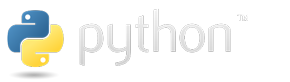
\includegraphics[keepaspectratio]{index_files/mediabag/python-logo.png}}

}

\caption{Python}

\end{figure}%

La Programación Orientada a Objetos (POO) es un paradigma de
programación que utiliza objetos y sus interacciones para diseñar
aplicaciones y programas de computadora. Está basado en varias técnicas,
incluyendo herencia, encapsulación, polimorfismo y abstracción.

Su sintaxis es más clara y sencilla de entender que otros paradigmas de
programación. Al permitirnos modelar entidades del mundo real de forma
más directa.

Ejemplo:

\begin{Shaded}
\begin{Highlighting}[]
\KeywordTok{class}\NormalTok{ Coche:}
    \KeywordTok{def} \FunctionTok{\_\_init\_\_}\NormalTok{(}\VariableTok{self}\NormalTok{, marca, modelo, color):}
        \VariableTok{self}\NormalTok{.marca }\OperatorTok{=}\NormalTok{ marca}
        \VariableTok{self}\NormalTok{.modelo }\OperatorTok{=}\NormalTok{ modelo}
        \VariableTok{self}\NormalTok{.color }\OperatorTok{=}\NormalTok{ color}

    \KeywordTok{def}\NormalTok{ acelerar(}\VariableTok{self}\NormalTok{):}
        \BuiltInTok{print}\NormalTok{(}\SpecialStringTok{f"El coche }\SpecialCharTok{\{}\VariableTok{self}\SpecialCharTok{.}\NormalTok{marca}\SpecialCharTok{\}}\SpecialStringTok{ }\SpecialCharTok{\{}\VariableTok{self}\SpecialCharTok{.}\NormalTok{modelo}\SpecialCharTok{\}}\SpecialStringTok{ de color }\SpecialCharTok{\{}\VariableTok{self}\SpecialCharTok{.}\NormalTok{color}\SpecialCharTok{\}}\SpecialStringTok{ está acelerando"}\NormalTok{)}

    \KeywordTok{def}\NormalTok{ frenar(}\VariableTok{self}\NormalTok{):}
        \BuiltInTok{print}\NormalTok{(}\SpecialStringTok{f"El coche }\SpecialCharTok{\{}\VariableTok{self}\SpecialCharTok{.}\NormalTok{marca}\SpecialCharTok{\}}\SpecialStringTok{ }\SpecialCharTok{\{}\VariableTok{self}\SpecialCharTok{.}\NormalTok{modelo}\SpecialCharTok{\}}\SpecialStringTok{ de color }\SpecialCharTok{\{}\VariableTok{self}\SpecialCharTok{.}\NormalTok{color}\SpecialCharTok{\}}\SpecialStringTok{ está frenando"}\NormalTok{)}

    \KeywordTok{def} \FunctionTok{\_\_str\_\_}\NormalTok{(}\VariableTok{self}\NormalTok{):}
        \ControlFlowTok{return} \SpecialStringTok{f"Coche }\SpecialCharTok{\{}\VariableTok{self}\SpecialCharTok{.}\NormalTok{marca}\SpecialCharTok{\}}\SpecialStringTok{ }\SpecialCharTok{\{}\VariableTok{self}\SpecialCharTok{.}\NormalTok{modelo}\SpecialCharTok{\}}\SpecialStringTok{ de color }\SpecialCharTok{\{}\VariableTok{self}\SpecialCharTok{.}\NormalTok{color}\SpecialCharTok{\}}\SpecialStringTok{"}
\end{Highlighting}
\end{Shaded}

En el código anterior se define una clase \textbf{Coche} con tres
atributos \textbf{marca}, \textbf{modelo} y \textbf{color}. Además, se
definen tres métodos \textbf{acelerar}, \textbf{frenar} y
\textbf{\textbf{str}}. El método \textbf{\textbf{str}} es un método
especial que se llama cuando se convierte un objeto a una cadena de
texto.

Para crear un objeto de la clase \textbf{Coche} se hace de la siguiente
manera:

\begin{Shaded}
\begin{Highlighting}[]
\NormalTok{coche }\OperatorTok{=}\NormalTok{ Coche(}\StringTok{"Toyota"}\NormalTok{, }\StringTok{"Corolla"}\NormalTok{, }\StringTok{"Rojo"}\NormalTok{)}
\BuiltInTok{print}\NormalTok{(coche)}
\NormalTok{coche.acelerar()}
\NormalTok{coche.frenar()}
\end{Highlighting}
\end{Shaded}

En el código anterior se crea un objeto \textbf{coche} de la clase
\textbf{Coche} con los atributos \textbf{Toyota}, \textbf{Corolla} y
\textbf{Rojo}. Luego se imprime el objeto \textbf{coche} y se llama a
los métodos \textbf{acelerar} y \textbf{frenar}.

\section{Objetos y Clases}\label{objetos-y-clases}

Los objetos son instancias de una clase. Una clase es una plantilla para
crear objetos. Los objetos tienen atributos y métodos.

\section{Atributos}\label{atributos}

Los atributos son variables que pertenecen a un objeto. Los atributos
pueden ser de cualquier tipo de datos.

Ejemplo:

\begin{Shaded}
\begin{Highlighting}[]
\KeywordTok{class}\NormalTok{ Coche:}
    \KeywordTok{def} \FunctionTok{\_\_init\_\_}\NormalTok{(}\VariableTok{self}\NormalTok{, marca, modelo, color):}
        \VariableTok{self}\NormalTok{.marca }\OperatorTok{=}\NormalTok{ marca}
        \VariableTok{self}\NormalTok{.modelo }\OperatorTok{=}\NormalTok{ modelo}
        \VariableTok{self}\NormalTok{.color }\OperatorTok{=}\NormalTok{ color}
\end{Highlighting}
\end{Shaded}

En el código anterior se definen tres atributos \textbf{marca},
\textbf{modelo} y \textbf{color}.

\section{¿Qué es self?}\label{quuxe9-es-self}

Self es una palabra reservada en Python que se refiere al objeto actual.
Se utiliza para acceder a los atributos y métodos de un objeto.

En el ejemplo anterior, \textbf{self.marca}, \textbf{self.modelo} y
\textbf{self.color} se refieren a los atributos de un objeto.

Ejemplo:

\begin{Shaded}
\begin{Highlighting}[]
\KeywordTok{class}\NormalTok{ Persona:}
    \KeywordTok{def} \FunctionTok{\_\_init\_\_}\NormalTok{(}\VariableTok{self}\NormalTok{, nombre, edad):}
        \VariableTok{self}\NormalTok{.nombre }\OperatorTok{=}\NormalTok{ nombre}
        \VariableTok{self}\NormalTok{.edad }\OperatorTok{=}\NormalTok{ edad}
    \KeywordTok{def}\NormalTok{ saludar(}\VariableTok{self}\NormalTok{):}
        \BuiltInTok{print}\NormalTok{(}\SpecialStringTok{f"Hola, mi nombre es }\SpecialCharTok{\{}\VariableTok{self}\SpecialCharTok{.}\NormalTok{nombre}\SpecialCharTok{\}}\SpecialStringTok{ y tengo }\SpecialCharTok{\{}\VariableTok{self}\SpecialCharTok{.}\NormalTok{edad}\SpecialCharTok{\}}\SpecialStringTok{ años"}\NormalTok{)}
\end{Highlighting}
\end{Shaded}

En el ejemplo anterior se define una clase \textbf{Persona} con dos
atributos \textbf{nombre} y \textbf{edad}. Además, se define un método
\textbf{saludar} que imprime un mensaje con los atributos
\textbf{nombre} y \textbf{edad}.

\section{Métodos}\label{muxe9todos}

Los métodos son funciones que pertenecen a un objeto. Los métodos pueden
acceder a los atributos de un objeto.

Ejemplo:

\begin{Shaded}
\begin{Highlighting}[]
\KeywordTok{class}\NormalTok{ Coche:}
    \KeywordTok{def}\NormalTok{ acelerar(}\VariableTok{self}\NormalTok{):}
        \BuiltInTok{print}\NormalTok{(}\SpecialStringTok{f"El coche }\SpecialCharTok{\{}\VariableTok{self}\SpecialCharTok{.}\NormalTok{marca}\SpecialCharTok{\}}\SpecialStringTok{ }\SpecialCharTok{\{}\VariableTok{self}\SpecialCharTok{.}\NormalTok{modelo}\SpecialCharTok{\}}\SpecialStringTok{ de color }\SpecialCharTok{\{}\VariableTok{self}\SpecialCharTok{.}\NormalTok{color}\SpecialCharTok{\}}\SpecialStringTok{ está acelerando"}\NormalTok{)}

    \KeywordTok{def}\NormalTok{ frenar(}\VariableTok{self}\NormalTok{):}
        \BuiltInTok{print}\NormalTok{(}\SpecialStringTok{f"El coche }\SpecialCharTok{\{}\VariableTok{self}\SpecialCharTok{.}\NormalTok{marca}\SpecialCharTok{\}}\SpecialStringTok{ }\SpecialCharTok{\{}\VariableTok{self}\SpecialCharTok{.}\NormalTok{modelo}\SpecialCharTok{\}}\SpecialStringTok{ de color }\SpecialCharTok{\{}\VariableTok{self}\SpecialCharTok{.}\NormalTok{color}\SpecialCharTok{\}}\SpecialStringTok{ está frenando"}\NormalTok{)}
\end{Highlighting}
\end{Shaded}

En el código anterior se definen dos métodos \textbf{acelerar} y
\textbf{frenar}.

\section{Self, Eliminar Propiedades y
Objetos}\label{self-eliminar-propiedades-y-objetos}

El primer parámetro de un método es \textbf{self}. \textbf{Self} es una
referencia al objeto actual. Se utiliza para acceder a los atributos y
métodos de un objeto.

Ejemplo:

\begin{Shaded}
\begin{Highlighting}[]
\KeywordTok{class}\NormalTok{ Coche:}
    \KeywordTok{def} \FunctionTok{\_\_init\_\_}\NormalTok{(}\VariableTok{self}\NormalTok{, marca, modelo, color):}
        \VariableTok{self}\NormalTok{.marca }\OperatorTok{=}\NormalTok{ marca}
        \VariableTok{self}\NormalTok{.modelo }\OperatorTok{=}\NormalTok{ modelo}
        \VariableTok{self}\NormalTok{.color }\OperatorTok{=}\NormalTok{ color}

    \KeywordTok{def}\NormalTok{ acelerar(}\VariableTok{self}\NormalTok{):}
        \BuiltInTok{print}\NormalTok{(}\SpecialStringTok{f"El coche }\SpecialCharTok{\{}\VariableTok{self}\SpecialCharTok{.}\NormalTok{marca}\SpecialCharTok{\}}\SpecialStringTok{ }\SpecialCharTok{\{}\VariableTok{self}\SpecialCharTok{.}\NormalTok{modelo}\SpecialCharTok{\}}\SpecialStringTok{ de color }\SpecialCharTok{\{}\VariableTok{self}\SpecialCharTok{.}\NormalTok{color}\SpecialCharTok{\}}\SpecialStringTok{ está acelerando"}\NormalTok{)}

    \KeywordTok{def}\NormalTok{ frenar(}\VariableTok{self}\NormalTok{):}
        \BuiltInTok{print}\NormalTok{(}\SpecialStringTok{f"El coche }\SpecialCharTok{\{}\VariableTok{self}\SpecialCharTok{.}\NormalTok{marca}\SpecialCharTok{\}}\SpecialStringTok{ }\SpecialCharTok{\{}\VariableTok{self}\SpecialCharTok{.}\NormalTok{modelo}\SpecialCharTok{\}}\SpecialStringTok{ de color }\SpecialCharTok{\{}\VariableTok{self}\SpecialCharTok{.}\NormalTok{color}\SpecialCharTok{\}}\SpecialStringTok{ está frenando"}\NormalTok{)}

    \KeywordTok{def} \FunctionTok{\_\_del\_\_}\NormalTok{(}\VariableTok{self}\NormalTok{):}
        \BuiltInTok{print}\NormalTok{(}\SpecialStringTok{f"El coche }\SpecialCharTok{\{}\VariableTok{self}\SpecialCharTok{.}\NormalTok{marca}\SpecialCharTok{\}}\SpecialStringTok{ }\SpecialCharTok{\{}\VariableTok{self}\SpecialCharTok{.}\NormalTok{modelo}\SpecialCharTok{\}}\SpecialStringTok{ de color }\SpecialCharTok{\{}\VariableTok{self}\SpecialCharTok{.}\NormalTok{color}\SpecialCharTok{\}}\SpecialStringTok{ ha sido eliminado"}\NormalTok{)}

\NormalTok{coche }\OperatorTok{=}\NormalTok{ Coche(}\StringTok{"Toyota"}\NormalTok{, }\StringTok{"Corolla"}\NormalTok{, }\StringTok{"Rojo"}\NormalTok{)}
\BuiltInTok{print}\NormalTok{(coche)}
\NormalTok{coche.acelerar()}
\NormalTok{coche.frenar()}
\KeywordTok{del}\NormalTok{ coche}
\end{Highlighting}
\end{Shaded}

En el código anterior se define un método especial \textbf{\textbf{del}}
que se llama cuando un objeto es eliminado. Luego se crea un objeto
\textbf{coche} de la clase \textbf{Coche} y se elimina el objeto
\textbf{coche}.

Por otra parte la palabra reservada \textbf{self} se utiliza para
acceder a los atributos y métodos de un objeto.

Tambien se está creando una instancia de la clase \textbf{Coche} y se
está eliminando el objeto \textbf{coche}.

\section{Eliminar Propiedades y
Objetos}\label{eliminar-propiedades-y-objetos}

Para eliminar Propiedades y Objetos se utiliza la palabra reservada
\textbf{del}.

Como observamos en el código anterior la propiedad \textbf{\textbf{del}}
se utiliza para eliminar un objeto.

Ejemplo:

\begin{Shaded}
\begin{Highlighting}[]
\KeywordTok{class}\NormalTok{ Persona:}
    \KeywordTok{def} \FunctionTok{\_\_init\_\_}\NormalTok{(}\VariableTok{self}\NormalTok{, nombre, edad):}
        \VariableTok{self}\NormalTok{.nombre }\OperatorTok{=}\NormalTok{ nombre}
        \VariableTok{self}\NormalTok{.edad }\OperatorTok{=}\NormalTok{ edad}
    \KeywordTok{def} \FunctionTok{\_\_del\_\_}\NormalTok{(}\VariableTok{self}\NormalTok{):}
        \BuiltInTok{print}\NormalTok{(}\SpecialStringTok{f"La persona }\SpecialCharTok{\{}\VariableTok{self}\SpecialCharTok{.}\NormalTok{nombre}\SpecialCharTok{\}}\SpecialStringTok{ ha sido eliminada"}\NormalTok{)}

\NormalTok{persona }\OperatorTok{=}\NormalTok{ Persona(}\StringTok{"Juan Perez"}\NormalTok{, }\DecValTok{30}\NormalTok{)}
\BuiltInTok{print}\NormalTok{(persona)}
\KeywordTok{del}\NormalTok{ persona}
\end{Highlighting}
\end{Shaded}

En el código anterior se define un método especial \textbf{\textbf{del}}
que se llama cuando un objeto es eliminado. Luego se crea un objeto
\textbf{persona} de la clase \textbf{Persona} y se elimina el objeto
\textbf{persona}. Al final obtendremos un mensaje como este:

\begin{Shaded}
\begin{Highlighting}[]
\NormalTok{La persona Juan Perez ha sido eliminada}
\end{Highlighting}
\end{Shaded}

\section{Herencia, Polimorfismo y
Encapsulación}\label{herencia-polimorfismo-y-encapsulaciuxf3n}

\subsection{Herencia}\label{herencia}

La herencia es una característica de la POO que permite crear una nueva
clase a partir de una clase existente. La nueva clase hereda los
atributos y métodos de la clase existente.

Ejemplo:

\begin{Shaded}
\begin{Highlighting}[]
\KeywordTok{class}\NormalTok{ Animal:}
    \KeywordTok{def} \FunctionTok{\_\_init\_\_}\NormalTok{(}\VariableTok{self}\NormalTok{, nombre):}
        \VariableTok{self}\NormalTok{.nombre }\OperatorTok{=}\NormalTok{ nombre}
    \KeywordTok{def}\NormalTok{ hablar(}\VariableTok{self}\NormalTok{):}
        \ControlFlowTok{pass}

\KeywordTok{class}\NormalTok{ Perro(Animal):}
    \KeywordTok{def}\NormalTok{ hablar(}\VariableTok{self}\NormalTok{):}
        \BuiltInTok{print}\NormalTok{(}\SpecialStringTok{f"}\SpecialCharTok{\{}\VariableTok{self}\SpecialCharTok{.}\NormalTok{nombre}\SpecialCharTok{\}}\SpecialStringTok{ dice guau"}\NormalTok{)}

\KeywordTok{class}\NormalTok{ Gato(Animal):}
    \KeywordTok{def}\NormalTok{ hablar(}\VariableTok{self}\NormalTok{):}
      \BuiltInTok{print}\NormalTok{(}\SpecialStringTok{f"}\SpecialCharTok{\{}\VariableTok{self}\SpecialCharTok{.}\NormalTok{nombre}\SpecialCharTok{\}}\SpecialStringTok{ dice miau"}\NormalTok{)}


\NormalTok{animal }\OperatorTok{=}\NormalTok{ Perro(}\StringTok{"Firulais"}\NormalTok{)}
\NormalTok{animal2 }\OperatorTok{=}\NormalTok{ Gato(}\StringTok{"Garfield"}\NormalTok{)}
\end{Highlighting}
\end{Shaded}

En el código anterior se define una clase \textbf{Animal} con un método
\textbf{hablar}. Luego se definen dos clases \textbf{Perro} y
\textbf{Gato} que heredan de la clase \textbf{Animal} y sobrescriben el
método \textbf{hablar}.

\subsection{Polimorfismo}\label{polimorfismo}

El polimorfismo es una característica de la POO que permite que un
objeto se computadora de diferentes maneras dependiendo del contexto.

Ejemplo:

\begin{Shaded}
\begin{Highlighting}[]
\KeywordTok{class}\NormalTok{ Deporte:}
    \KeywordTok{def}\NormalTok{ jugar(}\VariableTok{self}\NormalTok{):}
        \ControlFlowTok{pass}

\KeywordTok{class}\NormalTok{ Futbol(Deporte):}
    \KeywordTok{def}\NormalTok{ jugar(}\VariableTok{self}\NormalTok{):}
        \BuiltInTok{print}\NormalTok{(}\SpecialStringTok{f"Jugando futbol"}\NormalTok{)}

\KeywordTok{class}\NormalTok{ Baloncesto(Deporte):}
    \KeywordTok{def}\NormalTok{ jugar(}\VariableTok{self}\NormalTok{):}
      \BuiltInTok{print}\NormalTok{(}\SpecialStringTok{f"Jugando baloncesto"}\NormalTok{)}

\KeywordTok{class}\NormalTok{ Tenis(Deporte):}
    \KeywordTok{def}\NormalTok{ jugar(}\VariableTok{self}\NormalTok{):}
      \BuiltInTok{print}\NormalTok{(}\SpecialStringTok{f"Jugando tenis"}\NormalTok{)}

\NormalTok{deporte }\OperatorTok{=}\NormalTok{ Futbol()}
\NormalTok{deporte.jugar()}

\NormalTok{deporte1 }\OperatorTok{=}\NormalTok{ Baloncesto()}
\NormalTok{deporte1.jugar()}

\NormalTok{deporte2 }\OperatorTok{=}\NormalTok{ Tenis()}
\NormalTok{deporte2.jugar()}
\end{Highlighting}
\end{Shaded}

En el ejemplo anterior se define una clase \textbf{Deporte} con un
método \textbf{jugar}. Luego se definen tres clases \textbf{Futbol},
\textbf{Baloncesto} y \textbf{Tenis} que heredan de la clase
\textbf{Deporte} y sobrescriben el método \textbf{jugar}. Aunque los
tres objetos son de la clase \textbf{Deporte}, se comportan de manera
diferente.

\subsection{Encapsulación}\label{encapsulaciuxf3n}

La encapsulación es una característica de la POO que permite ocultar los
detalles de implementación de un objeto. Los atributos y métodos de un
objeto pueden ser públicos, protegidos o privados.

Ejemplo:

\begin{Shaded}
\begin{Highlighting}[]
\KeywordTok{class}\NormalTok{ CuentaBancaria:}
    \KeywordTok{def} \FunctionTok{\_\_init\_\_}\NormalTok{(}\VariableTok{self}\NormalTok{, nombre, saldo):}
        \VariableTok{self}\NormalTok{.nombre }\OperatorTok{=}\NormalTok{ nombre}
        \VariableTok{self}\NormalTok{.\_\_saldo }\OperatorTok{=}\NormalTok{ saldo  }\CommentTok{\# El saldo es privado}

    \KeywordTok{def}\NormalTok{ depositar(}\VariableTok{self}\NormalTok{, cantidad):}
        \VariableTok{self}\NormalTok{.\_\_saldo }\OperatorTok{+=}\NormalTok{ cantidad}

    \KeywordTok{def}\NormalTok{ retirar(}\VariableTok{self}\NormalTok{, cantidad):}
        \ControlFlowTok{if}\NormalTok{ cantidad }\OperatorTok{\textless{}=} \VariableTok{self}\NormalTok{.\_\_saldo:}
            \VariableTok{self}\NormalTok{.\_\_saldo }\OperatorTok{{-}=}\NormalTok{ cantidad}
        \ControlFlowTok{else}\NormalTok{:}
            \BuiltInTok{print}\NormalTok{(}\StringTok{"Fondos insuficientes"}\NormalTok{)}

    \KeywordTok{def}\NormalTok{ obtener\_saldo(}\VariableTok{self}\NormalTok{):}
        \ControlFlowTok{return} \VariableTok{self}\NormalTok{.\_\_saldo  }\CommentTok{\# Método para acceder al saldo}

    \KeywordTok{def} \FunctionTok{\_\_str\_\_}\NormalTok{(}\VariableTok{self}\NormalTok{):}
        \ControlFlowTok{return} \SpecialStringTok{f"Cuenta Bancaria de }\SpecialCharTok{\{}\VariableTok{self}\SpecialCharTok{.}\NormalTok{nombre}\SpecialCharTok{\}}\SpecialStringTok{ con saldo }\SpecialCharTok{\{}\VariableTok{self}\SpecialCharTok{.}\NormalTok{\_\_saldo}\SpecialCharTok{\}}\SpecialStringTok{"}


\CommentTok{\# Creación de instancias de cuentas bancarias}
\NormalTok{cuenta1 }\OperatorTok{=}\NormalTok{ CuentaBancaria(}\StringTok{"Juan Perez"}\NormalTok{, }\DecValTok{1000}\NormalTok{)}
\NormalTok{cuenta2 }\OperatorTok{=}\NormalTok{ CuentaBancaria(}\StringTok{"Maria Lopez"}\NormalTok{, }\DecValTok{2000}\NormalTok{)}
\NormalTok{cuenta3 }\OperatorTok{=}\NormalTok{ CuentaBancaria(}\StringTok{"Pedro Ramirez"}\NormalTok{, }\DecValTok{3000}\NormalTok{)}

\CommentTok{\# Operaciones en las cuentas}
\NormalTok{cuenta1.depositar(}\DecValTok{500}\NormalTok{)}
\NormalTok{cuenta1.retirar(}\DecValTok{200}\NormalTok{)}
\BuiltInTok{print}\NormalTok{(cuenta1.nombre)}
\BuiltInTok{print}\NormalTok{(cuenta1.obtener\_saldo())  }\CommentTok{\# Acceso al saldo a través de un método}

\BuiltInTok{print}\NormalTok{(cuenta2.nombre)}
\NormalTok{cuenta2.depositar(}\DecValTok{500}\NormalTok{)}
\NormalTok{cuenta2.retirar(}\DecValTok{200}\NormalTok{)}
\BuiltInTok{print}\NormalTok{(cuenta2.obtener\_saldo())}

\BuiltInTok{print}\NormalTok{(cuenta3.nombre)}
\NormalTok{cuenta3.depositar(}\DecValTok{1000}\NormalTok{)}
\NormalTok{cuenta3.retirar(}\DecValTok{500}\NormalTok{)}
\BuiltInTok{print}\NormalTok{(cuenta3.obtener\_saldo())}
\end{Highlighting}
\end{Shaded}

La encapsulación es un principio fundamental en la programación
orientada a objetos que permite proteger los datos de un objeto. En
Python, se logra utilizando variables privadas y métodos de acceso para
controlar cómo se accede y modifica la información dentro de una clase.

En el ejemplo de CuentaBancaria, el atributo \textbf{saldo es privado
(indicado por el prefijo }) y no puede ser accedido directamente desde
fuera de la clase. Esto significa que no se puede escribir
cuenta1.\_\_saldo para leer o modificar el saldo.

Para interactuar con el saldo de manera segura, la clase proporciona
métodos públicos como depositar y retirar, que permiten modificar el
saldo solo bajo condiciones controladas. En este caso, se agregó un
método obtener\_saldo para acceder al saldo de manera segura. Este
enfoque evita que se altere el saldo de forma indebida y permite
implementar lógica adicional, como verificar si hay fondos suficientes
antes de retirar una cantidad.

Este ejemplo demuestra cómo la encapsulación ayuda a proteger y
controlar el acceso a los datos de un objeto, asegurando que su estado
interno se gestione correctamente.

\section{Actividad}\label{actividad-4}

\begin{enumerate}
\def\labelenumi{\arabic{enumi}.}
\item
  Crear una clase \textbf{Persona} con los atributos \textbf{nombre},
  \textbf{edad} y \textbf{sexo}.
\item
  Crear una clase \textbf{Estudiante} que herede de la clase
  \textbf{Persona} con los atributos \textbf{carnet} y \textbf{carrera}.
\item
  Crear una clase \textbf{Profesor} que herede de la clase
  \textbf{Persona} con los atributos \textbf{codigo} y
  \textbf{especialidad}.
\item
  Crear una clase \textbf{Curso} con los atributos \textbf{nombre},
  \textbf{codigo} y \textbf{profesor}.
\item
  Crear una clase \textbf{Universidad} con los atributos \textbf{nombre}
  y \textbf{cursos}.
\item
  Crear un objeto \textbf{universidad} de la clase \textbf{Universidad}
  con el nombre \textbf{Universidad de El Salvador} y los siguientes
  cursos:
\end{enumerate}

\begin{itemize}
\tightlist
\item
  \textbf{Curso 1}: Nombre: \textbf{Matematicas}, Codigo:
  \textbf{MAT101}, Profesor: \textbf{Juan Perez}
\item
  \textbf{Curso 2}: Nombre: \textbf{Fisica}, Codigo: \textbf{FIS101},
  Profesor: \textbf{Maria Lopez}
\item
  \textbf{Curso 3}: Nombre: \textbf{Quimica}, Codigo: \textbf{QUI101},
  Profesor: \textbf{Pedro Ramirez}
\end{itemize}

\begin{enumerate}
\def\labelenumi{\arabic{enumi}.}
\setcounter{enumi}{6}
\item
  Imprimir el objeto \textbf{universidad}.
\item
  Crear un objeto \textbf{estudiante} de la clase \textbf{Estudiante}
  con los siguientes atributos:
\end{enumerate}

\begin{itemize}
\item
  Nombre: \textbf{Carlos Perez}
\item
  Edad: \textbf{20}
\item
  Sexo: \textbf{Masculino}
\item
  Carnet: \textbf{202010101}
\item
  Carrera: \textbf{Ingenieria en Sistemas Informaticos}
\end{itemize}

\begin{enumerate}
\def\labelenumi{\arabic{enumi}.}
\setcounter{enumi}{8}
\item
  Imprimir el objeto \textbf{estudiante}.
\item
  Crear un objeto \textbf{profesor} de la clase \textbf{Profesor} con
  los siguientes atributos:
\end{enumerate}

\begin{itemize}
\item
  Nombre: \textbf{Juan Perez}
\item
  Edad: \textbf{30}
\item
  Sexo: \textbf{Masculino}
\item
  Codigo: \textbf{202020202}
\item
  Especialidad: \textbf{Matematicas}
\end{itemize}

\begin{enumerate}
\def\labelenumi{\arabic{enumi}.}
\setcounter{enumi}{10}
\item
  Imprimir el objeto \textbf{profesor}.
\item
  Crear un objeto \textbf{curso} de la clase \textbf{Curso} con los
  siguientes atributos:
\end{enumerate}

\begin{itemize}
\item
  Nombre: \textbf{Matematicas}
\item
  Codigo: \textbf{MAT101}
\item
  Profesor: \textbf{Juan Perez}
\end{itemize}

\begin{enumerate}
\def\labelenumi{\arabic{enumi}.}
\setcounter{enumi}{12}
\item
  Imprimir el objeto \textbf{curso}.
\item
  Agregar el objeto \textbf{curso} al objeto \textbf{universidad}.
\item
  Imprimir el objeto \textbf{universidad}.
\item
  Crear un objeto \textbf{curso} de la clase \textbf{Curso} con los
  siguientes atributos:
\end{enumerate}

\begin{itemize}
\item
  Nombre: \textbf{Fisica}
\item
  Codigo: \textbf{FIS101}
\item
  Profesor: \textbf{Maria Lopez}
\end{itemize}

Respuesta

\begin{Shaded}
\begin{Highlighting}[]
\KeywordTok{class}\NormalTok{ Persona:}
    \KeywordTok{def} \FunctionTok{\_\_init\_\_}\NormalTok{(}\VariableTok{self}\NormalTok{, nombre, edad, sexo):}
        \VariableTok{self}\NormalTok{.nombre }\OperatorTok{=}\NormalTok{ nombre}
        \VariableTok{self}\NormalTok{.edad }\OperatorTok{=}\NormalTok{ edad}
        \VariableTok{self}\NormalTok{.sexo }\OperatorTok{=}\NormalTok{ sexo}

\KeywordTok{class}\NormalTok{ Estudiante(Persona):}
    \KeywordTok{def} \FunctionTok{\_\_init\_\_}\NormalTok{(}\VariableTok{self}\NormalTok{, nombre, edad, sexo, carnet, carrera):}
        \BuiltInTok{super}\NormalTok{().}\FunctionTok{\_\_init\_\_}\NormalTok{(nombre, edad, sexo)}
        \VariableTok{self}\NormalTok{.carnet }\OperatorTok{=}\NormalTok{ carnet}
        \VariableTok{self}\NormalTok{.carrera }\OperatorTok{=}\NormalTok{ carrera}

\KeywordTok{class}\NormalTok{ Profesor(Persona):}
    \KeywordTok{def} \FunctionTok{\_\_init\_\_}\NormalTok{(}\VariableTok{self}\NormalTok{, nombre, edad, sexo, codigo, especialidad):}
        \BuiltInTok{super}\NormalTok{().}\FunctionTok{\_\_init\_\_}\NormalTok{(nombre, edad, sexo)}
        \VariableTok{self}\NormalTok{.codigo }\OperatorTok{=}\NormalTok{ codigo}
        \VariableTok{self}\NormalTok{.especialidad }\OperatorTok{=}\NormalTok{ especialidad}

\KeywordTok{class}\NormalTok{ Curso:}
    \KeywordTok{def} \FunctionTok{\_\_init\_\_}\NormalTok{(}\VariableTok{self}\NormalTok{, nombre, codigo, profesor):}
        \VariableTok{self}\NormalTok{.nombre }\OperatorTok{=}\NormalTok{ nombre}
        \VariableTok{self}\NormalTok{.codigo }\OperatorTok{=}\NormalTok{ codigo}
        \VariableTok{self}\NormalTok{.profesor }\OperatorTok{=}\NormalTok{ profesor}

\KeywordTok{class}\NormalTok{ Universidad}
    \KeywordTok{def} \FunctionTok{\_\_init\_\_}\NormalTok{(}\VariableTok{self}\NormalTok{, nombre):}
        \VariableTok{self}\NormalTok{.nombre }\OperatorTok{=}\NormalTok{ nombre}
        \VariableTok{self}\NormalTok{.cursos }\OperatorTok{=}\NormalTok{ []}

\NormalTok{universidad }\OperatorTok{=}\NormalTok{ Universidad(}\StringTok{"Universidad de las Fuerzas Armadas ESPE"}\NormalTok{)}
\NormalTok{curso1 }\OperatorTok{=}\NormalTok{ Curso(}\StringTok{"Matematicas"}\NormalTok{, }\StringTok{"MAT101"}\NormalTok{, }\StringTok{"Juan Perez"}\NormalTok{)}
\NormalTok{curso2 }\OperatorTok{=}\NormalTok{ Curso(}\StringTok{"Fisica"}\NormalTok{, }\StringTok{"FIS101"}\NormalTok{, }\StringTok{"Maria Lopez"}\NormalTok{)}
\NormalTok{curso3 }\OperatorTok{=}\NormalTok{ Curso(}\StringTok{"Quimica"}\NormalTok{, }\StringTok{"QUI101"}\NormalTok{, }\StringTok{"Pedro Ramirez"}\NormalTok{)}
\NormalTok{universidad.cursos.append(curso1)}
\NormalTok{universidad.cursos.append(curso2)}
\NormalTok{universidad.cursos.append(curso3)}
\BuiltInTok{print}\NormalTok{(universidad)}

\NormalTok{estudiante }\OperatorTok{=}\NormalTok{ Estudiante(}\StringTok{"Carlos Perez"}\NormalTok{, }\DecValTok{20}\NormalTok{, }\StringTok{"Masculino"}\NormalTok{, }\StringTok{"202010101"}\NormalTok{, }\StringTok{"Ingenieria en Sistemas Informaticos"}\NormalTok{)}
\BuiltInTok{print}\NormalTok{(estudiante)}

\NormalTok{profesor }\OperatorTok{=}\NormalTok{ Profesor(}\StringTok{"Juan Perez"}\NormalTok{, }\DecValTok{30}\NormalTok{, }\StringTok{"Masculino"}\NormalTok{, }\StringTok{"202020202"}\NormalTok{, }\StringTok{"Matematicas"}\NormalTok{)}
\BuiltInTok{print}\NormalTok{(profesor)}

\NormalTok{curso }\OperatorTok{=}\NormalTok{ Curso(}\StringTok{"Matematicas"}\NormalTok{, }\StringTok{"MAT101"}\NormalTok{, }\StringTok{"Juan Perez"}\NormalTok{)}
\BuiltInTok{print}\NormalTok{(curso)}

\NormalTok{curso }\OperatorTok{=}\NormalTok{ Curso(}\StringTok{"Fisica"}\NormalTok{, }\StringTok{"FIS101"}\NormalTok{, }\StringTok{"Maria Lopez"}\NormalTok{)}
\NormalTok{universidad.cursos.append(curso)}
\BuiltInTok{print}\NormalTok{(universidad)}
\end{Highlighting}
\end{Shaded}

\chapter{Conclusiones}\label{conclusiones-4}

La Programación Orientada a Objetos (POO) es un paradigma de
programación que utiliza objetos y sus interacciones para diseñar
aplicaciones y programas de computadora. Está basado en varias técnicas,
incluyendo herencia, encapsulación, polimorfismo y abstracción.

\part{Unidad 3: Módulos y Paquetes}

\chapter{Módulos}\label{muxf3dulos}

\begin{figure}[H]

{\centering \pandocbounded{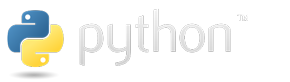
\includegraphics[keepaspectratio]{index_files/mediabag/python-logo.png}}

}

\caption{Python}

\end{figure}%

\section{Introducción a Módulos}\label{introducciuxf3n-a-muxf3dulos}

En Python, un módulo es un archivo que contiene código, generalmente
funciones, clases, y variables, que puedes importar y reutilizar en
diferentes partes de tu programa. Esto te ayuda a dividir tu código en
partes organizadas y reutilizables, haciendo que el desarrollo sea más
eficiente y limpio.

Por ejemplo, imagina que quieres crear un módulo para realizar saludos y
otro para despedidas:

Ejemplo 1: Módulo de saludo

\begin{Shaded}
\begin{Highlighting}[]
\CommentTok{\# modulo\_saludo.py}
\KeywordTok{def}\NormalTok{ saludar():}
    \BuiltInTok{print}\NormalTok{(}\StringTok{"Hola Mundo"}\NormalTok{)}
\end{Highlighting}
\end{Shaded}

Ejemplo 2: Módulo de despedida

\begin{Shaded}
\begin{Highlighting}[]
\CommentTok{\# modulo\_despedida.py}
\KeywordTok{def}\NormalTok{ despedir():}
    \BuiltInTok{print}\NormalTok{(}\StringTok{"Adiós Mundo"}\NormalTok{)}
\end{Highlighting}
\end{Shaded}

Estos módulos contienen funciones que realizan acciones específicas: uno
saluda y el otro se despide. Ahora veremos cómo crear y utilizar módulos
en Python.

\section{Creando Módulos
Personalizados}\label{creando-muxf3dulos-personalizados}

Para crear un módulo en Python, solo necesitas crear un archivo .py y
definir en él las funciones o clases que deseas usar. A continuación,
veamos cómo crear módulos más complejos.

Ejemplo: Módulo de saludo con nombre

\begin{Shaded}
\begin{Highlighting}[]
\CommentTok{\# modulo\_saludar.py}

\KeywordTok{def}\NormalTok{ saludar(nombre):}
    \BuiltInTok{print}\NormalTok{(}\SpecialStringTok{f"Hola, }\SpecialCharTok{\{}\NormalTok{nombre}\SpecialCharTok{\}}\SpecialStringTok{!"}\NormalTok{)}
\end{Highlighting}
\end{Shaded}

Este módulo acepta un argumento nombre, permitiéndote personalizar el
saludo.

\section{Usando Módulos en un Archivo
Principal}\label{usando-muxf3dulos-en-un-archivo-principal}

Para utilizar los módulos que has creado, necesitas importarlos en un
archivo principal. Aquí, importamos ambos módulos anteriores y
ejecutamos las funciones:

\begin{Shaded}
\begin{Highlighting}[]
\CommentTok{\# main.py}
\ImportTok{import}\NormalTok{ modulo\_saludar}
\ImportTok{import}\NormalTok{ modulo\_despedida}

\ControlFlowTok{if} \VariableTok{\_\_name\_\_} \OperatorTok{==} \StringTok{"\_\_main\_\_"}\NormalTok{:}
\NormalTok{    modulo\_saludar.saludar(}\StringTok{"Juan"}\NormalTok{)}
\NormalTok{    modulo\_despedida.despedir()}
\end{Highlighting}
\end{Shaded}

En este ejemplo, importamos los módulos modulo\_saludar y
modulo\_despedida y usamos las funciones saludar y despedir.

\section{Importando y Renombrando
Módulos}\label{importando-y-renombrando-muxf3dulos}

A veces, renombrar un módulo en el momento de importarlo hace el código
más claro. Esto se logra con la palabra clave as:

\begin{Shaded}
\begin{Highlighting}[]
\CommentTok{\# main.py}
\ImportTok{import}\NormalTok{ modulo\_saludar }\ImportTok{as}\NormalTok{ saludo}
\ImportTok{import}\NormalTok{ modulo\_despedida }\ImportTok{as}\NormalTok{ despedida}

\NormalTok{saludo.saludar(}\StringTok{"Ana"}\NormalTok{)}
\NormalTok{despedida.despedir()}
\end{Highlighting}
\end{Shaded}

Esto permite usar nombres cortos y descriptivos en el código.

\section{Importando Funciones Específicas de un
Módulo}\label{importando-funciones-especuxedficas-de-un-muxf3dulo}

Si solo necesitas una función de un módulo, puedes importarla
directamente:

\begin{Shaded}
\begin{Highlighting}[]
\ImportTok{from}\NormalTok{ modulo\_saludar }\ImportTok{import}\NormalTok{ saludar}

\NormalTok{saludar(}\StringTok{"Carlos"}\NormalTok{)}
\end{Highlighting}
\end{Shaded}

Aquí importamos únicamente la función saludar de modulo\_saludar, sin
necesidad de importar el módulo completo.

\section{Usando Módulos Externos con
pip}\label{usando-muxf3dulos-externos-con-pip}

Además de tus propios módulos, Python permite instalar y utilizar
módulos externos usando pip, el gestor de paquetes de Python. Veamos un
ejemplo con numpy, un módulo popular para trabajar con arreglos
numéricos.

\section{Instalando un módulo con
pip}\label{instalando-un-muxf3dulo-con-pip}

\begin{Shaded}
\begin{Highlighting}[]
\ExtensionTok{pip}\NormalTok{ install numpy}
\end{Highlighting}
\end{Shaded}

\section{Usando el módulo
instalado}\label{usando-el-muxf3dulo-instalado}

\begin{Shaded}
\begin{Highlighting}[]
\ImportTok{import}\NormalTok{ numpy }\ImportTok{as}\NormalTok{ np}

\NormalTok{a }\OperatorTok{=}\NormalTok{ np.array([}\DecValTok{1}\NormalTok{, }\DecValTok{2}\NormalTok{, }\DecValTok{3}\NormalTok{, }\DecValTok{4}\NormalTok{, }\DecValTok{5}\NormalTok{])}
\BuiltInTok{print}\NormalTok{(a)}
\end{Highlighting}
\end{Shaded}

Este ejemplo muestra cómo instalar y utilizar numpy para crear un
arreglo.

\section{Instalando otro módulo}\label{instalando-otro-muxf3dulo}

Además de numpy, Python tiene muchos módulos útiles para diferentes
tareas. Por ejemplo, emojis es un módulo que te permite imprimir emojis
en la consola.

\begin{Shaded}
\begin{Highlighting}[]
\ExtensionTok{pip}\NormalTok{ install emojis}
\end{Highlighting}
\end{Shaded}

\section{Usando el módulo emojis}\label{usando-el-muxf3dulo-emojis}

\begin{Shaded}
\begin{Highlighting}[]
\ImportTok{import}\NormalTok{ emojis}

\BuiltInTok{print}\NormalTok{(emojis.encode(}\StringTok{":smile:"}\NormalTok{))}
\end{Highlighting}
\end{Shaded}

Este ejemplo muestra cómo instalar y utilizar el módulo emojis para
imprimir emojis en la consola.

\begin{Shaded}
\begin{Highlighting}[]
\ExtensionTok{😄}
\end{Highlighting}
\end{Shaded}

\chapter{Actividad Práctica}\label{actividad-pruxe1ctica}

Sigue estos pasos para practicar la creación y uso de módulos en Python.

\begin{enumerate}
\def\labelenumi{\arabic{enumi}.}
\tightlist
\item
  Crear un módulo modulo\_calculadora.py que contenga las funciones
  sumar, restar, multiplicar, y dividir:
\end{enumerate}

Ver solución

\begin{Shaded}
\begin{Highlighting}[]
\CommentTok{\# modulo\_calculadora.py}

\KeywordTok{def}\NormalTok{ sumar(a, b):}
    \ControlFlowTok{return}\NormalTok{ a }\OperatorTok{+}\NormalTok{ b}

\KeywordTok{def}\NormalTok{ restar(a, b):}
    \ControlFlowTok{return}\NormalTok{ a }\OperatorTok{{-}}\NormalTok{ b}

\KeywordTok{def}\NormalTok{ multiplicar(a, b):}
    \ControlFlowTok{return}\NormalTok{ a }\OperatorTok{*}\NormalTok{ b}

\KeywordTok{def}\NormalTok{ dividir(a, b):}
    \ControlFlowTok{return}\NormalTok{ a }\OperatorTok{/}\NormalTok{ b}
\end{Highlighting}
\end{Shaded}

Crear un archivo main.py que importe el módulo modulo\_calculadora y
utilice sus funciones:

\begin{Shaded}
\begin{Highlighting}[]
\CommentTok{\# main.py}
\ImportTok{import}\NormalTok{ modulo\_calculadora}

\BuiltInTok{print}\NormalTok{(modulo\_calculadora.sumar(}\DecValTok{10}\NormalTok{, }\DecValTok{5}\NormalTok{))}
\BuiltInTok{print}\NormalTok{(modulo\_calculadora.restar(}\DecValTok{10}\NormalTok{, }\DecValTok{5}\NormalTok{))}
\BuiltInTok{print}\NormalTok{(modulo\_calculadora.multiplicar(}\DecValTok{10}\NormalTok{, }\DecValTok{5}\NormalTok{))}
\BuiltInTok{print}\NormalTok{(modulo\_calculadora.dividir(}\DecValTok{10}\NormalTok{, }\DecValTok{5}\NormalTok{))}
\end{Highlighting}
\end{Shaded}

\begin{enumerate}
\def\labelenumi{\arabic{enumi}.}
\setcounter{enumi}{1}
\tightlist
\item
  Instalar numpy y crear un archivo main\_numpy.py que lo use para crear
  un arreglo:
\end{enumerate}

Ver solución

\begin{Shaded}
\begin{Highlighting}[]
\CommentTok{\# main\_numpy.py}
\ImportTok{import}\NormalTok{ numpy }\ImportTok{as}\NormalTok{ np}

\NormalTok{a }\OperatorTok{=}\NormalTok{ np.array([}\DecValTok{1}\NormalTok{, }\DecValTok{2}\NormalTok{, }\DecValTok{3}\NormalTok{, }\DecValTok{4}\NormalTok{, }\DecValTok{5}\NormalTok{])}
\BuiltInTok{print}\NormalTok{(a)}
\end{Highlighting}
\end{Shaded}

Crear un archivo main\_pandas.py que utilice pandas para crear un
DataFrame y lo imprima:

\begin{Shaded}
\begin{Highlighting}[]
\CommentTok{\# main\_pandas.py}
\ImportTok{import}\NormalTok{ pandas }\ImportTok{as}\NormalTok{ pd}

\NormalTok{data }\OperatorTok{=}\NormalTok{ \{}\StringTok{\textquotesingle{}Nombre\textquotesingle{}}\NormalTok{: [}\StringTok{\textquotesingle{}Juan\textquotesingle{}}\NormalTok{, }\StringTok{\textquotesingle{}Ana\textquotesingle{}}\NormalTok{, }\StringTok{\textquotesingle{}Luis\textquotesingle{}}\NormalTok{], }\StringTok{\textquotesingle{}Edad\textquotesingle{}}\NormalTok{: [}\DecValTok{23}\NormalTok{, }\DecValTok{30}\NormalTok{, }\DecValTok{27}\NormalTok{]\}}
\NormalTok{df }\OperatorTok{=}\NormalTok{ pd.DataFrame(data)}
\BuiltInTok{print}\NormalTok{(df)}
\end{Highlighting}
\end{Shaded}

\begin{enumerate}
\def\labelenumi{\arabic{enumi}.}
\setcounter{enumi}{2}
\tightlist
\item
  Crear un archivo main\_matplotlib.py para graficar una función:
\end{enumerate}

Ver solución

\begin{Shaded}
\begin{Highlighting}[]
\CommentTok{\# main\_matplotlib.py}
\ImportTok{import}\NormalTok{ matplotlib.pyplot }\ImportTok{as}\NormalTok{ plt}
\ImportTok{import}\NormalTok{ numpy }\ImportTok{as}\NormalTok{ np}

\NormalTok{x }\OperatorTok{=}\NormalTok{ np.linspace(}\DecValTok{0}\NormalTok{, }\DecValTok{10}\NormalTok{, }\DecValTok{100}\NormalTok{)}
\NormalTok{y }\OperatorTok{=}\NormalTok{ np.sin(x)}

\NormalTok{plt.plot(x, y)}
\NormalTok{plt.show()}
\end{Highlighting}
\end{Shaded}

\begin{enumerate}
\def\labelenumi{\arabic{enumi}.}
\setcounter{enumi}{3}
\tightlist
\item
  Instalar el módulo emojis y crear un archivo main\_emojis.py que
  imprima emojis en la consola:
\end{enumerate}

Ver solución

\begin{Shaded}
\begin{Highlighting}[]
\CommentTok{\# main\_emojis.py}
\ImportTok{import}\NormalTok{ emojis}

\BuiltInTok{print}\NormalTok{(emojis.encode(}\StringTok{":smile:"}\NormalTok{))}
\BuiltInTok{print}\NormalTok{(emojis.encode(}\StringTok{":heart:"}\NormalTok{))}
\BuiltInTok{print}\NormalTok{(emojis.encode(}\StringTok{":rocket:"}\NormalTok{))}
\end{Highlighting}
\end{Shaded}

\chapter{Conclusión}\label{conclusiuxf3n-2}

Los módulos en Python son una herramienta poderosa para estructurar y
reutilizar código. Con módulos, puedes dividir tu código en archivos
independientes y organizados, lo cual facilita el desarrollo de
aplicaciones escalables y mantenibles.

\part{Unidad 4: Docker}

\chapter{Docker}\label{docker}

\begin{figure}[H]

{\centering 
\includegraphics[width=2.08333in,height=\textheight,keepaspectratio]{unidades/unidad4/./images/docker.png}

}

\caption{Docker}

\end{figure}%

Docker es una plataforma que permite desarrollar, enviar y ejecutar
aplicaciones en contenedores. Un \textbf{contenedor} es una instancia
ejecutable de una \textbf{imagen}, que es una especie de
\textbf{plantilla} que contiene todo lo necesario para ejecutar una
aplicación.

Haciendo una analogía con los contenedores de transporte, una
\textbf{imagen} sería el \textbf{contenedor} en sí, y el
\textbf{contenedor} sería la \textbf{carga} que se transporta.

Docker resuelve un problema principal en el desarrollo de software: la
\textbf{portabilidad}. Al empaquetar una aplicación y sus dependencias
en un contenedor, se garantiza que la aplicación se ejecute de manera
\textbf{consistente} en diferentes entornos.

En esta lección, aprenderemos a crear y ejecutar contenedores Docker, y
a utilizarlos para ejecutar aplicaciones de manera aislada y portátil.

Con docker se acaba la frase típica de los desarrolladores \textbf{En mi
máquina funciona}. Con Docker, puedes estar seguro de que tu aplicación
funcionará de la misma manera en cualquier entorno.

\pandocbounded{
\includegraphics[keepaspectratio]{unidades/unidad4/./images/docker_image.png}}

Una imagen Docker es una plantilla inmutable que contiene un conjunto de
instrucciones para crear un contenedor Docker. Las imágenes son
portátiles y pueden ser compartidas, almacenadas y actualizadas.

\begin{tcolorbox}[enhanced jigsaw, toptitle=1mm, titlerule=0mm, left=2mm, opacityback=0, coltitle=black, leftrule=.75mm, title=\textcolor{quarto-callout-tip-color}{\faLightbulb}\hspace{0.5em}{Tip}, bottomrule=.15mm, arc=.35mm, opacitybacktitle=0.6, bottomtitle=1mm, toprule=.15mm, colbacktitle=quarto-callout-tip-color!10!white, rightrule=.15mm, breakable, colframe=quarto-callout-tip-color-frame, colback=white]

Las imágenes Docker son inmutables, lo que significa que no se pueden
modificar una vez creadas. Si se realizan cambios en una imagen, se debe
crear una nueva versión de la imagen.

\end{tcolorbox}

\pandocbounded{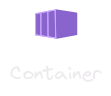
\includegraphics[keepaspectratio]{unidades/unidad4/./images/docker_container.png}}

Un contenedor Docker es una instancia ejecutable de una imagen Docker.
Se ejecuta de manera aislada y contiene todo lo necesario para ejecutar
la aplicación, incluyendo el código, las dependencias, el entorno de
ejecución, las bibliotecas y los archivos de configuración.

\begin{tcolorbox}[enhanced jigsaw, toptitle=1mm, titlerule=0mm, left=2mm, opacityback=0, coltitle=black, leftrule=.75mm, title=\textcolor{quarto-callout-tip-color}{\faLightbulb}\hspace{0.5em}{Tip}, bottomrule=.15mm, arc=.35mm, opacitybacktitle=0.6, bottomtitle=1mm, toprule=.15mm, colbacktitle=quarto-callout-tip-color!10!white, rightrule=.15mm, breakable, colframe=quarto-callout-tip-color-frame, colback=white]

Un contenedor aisla la aplicación de su entorno, lo que garantiza que la
aplicación se ejecute de manera consistente en diferentes entornos.

\end{tcolorbox}

\section{Ejemplos:}\label{ejemplos}

Descargar una imagen:

\begin{Shaded}
\begin{Highlighting}[]
\ExtensionTok{docker}\NormalTok{ pull docker/getting{-}started}
\end{Highlighting}
\end{Shaded}

\pandocbounded{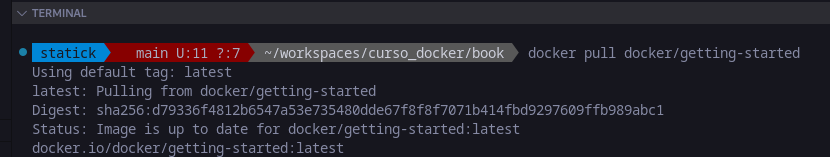
\includegraphics[keepaspectratio]{unidades/unidad4/images/paste-2.png}}

Este comando descarga la imagen \textbf{getting-started} desde el
registro público de Docker.

Correr un contenedor en el puerto 80:

\begin{Shaded}
\begin{Highlighting}[]
\ExtensionTok{docker}\NormalTok{ run }\AttributeTok{{-}d} \AttributeTok{{-}p}\NormalTok{ 80:80 docker/getting{-}started}
\end{Highlighting}
\end{Shaded}

\pandocbounded{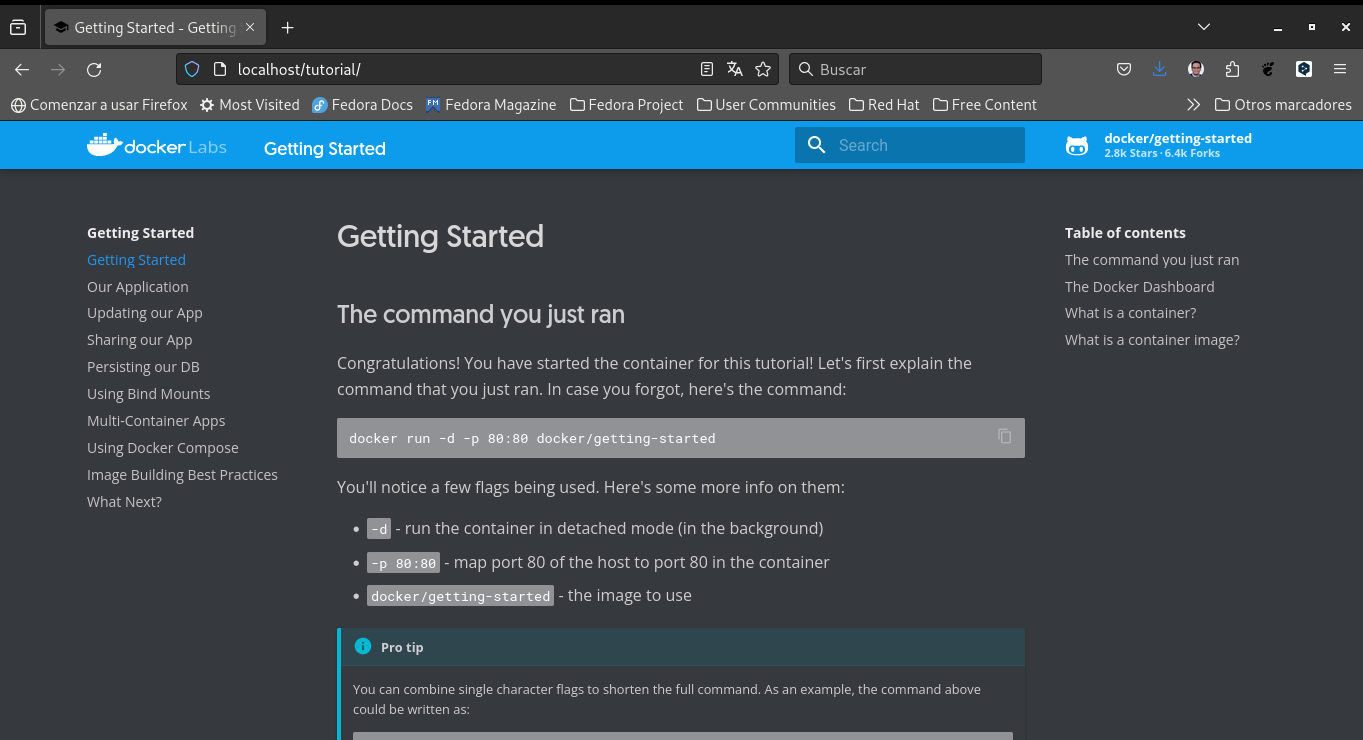
\includegraphics[keepaspectratio]{unidades/unidad4/images/paste-1.png}}

Este comando ejecuta un contenedor desenlazado en segundo plano (-d) y
mapea el puerto 80 de la máquina host al puerto 80 del contenedor (-p
80:80).

Descargar una imagen desde un registro.

\begin{tcolorbox}[enhanced jigsaw, toptitle=1mm, titlerule=0mm, left=2mm, opacityback=0, coltitle=black, leftrule=.75mm, title=\textcolor{quarto-callout-tip-color}{\faLightbulb}\hspace{0.5em}{Tip}, bottomrule=.15mm, arc=.35mm, opacitybacktitle=0.6, bottomtitle=1mm, toprule=.15mm, colbacktitle=quarto-callout-tip-color!10!white, rightrule=.15mm, breakable, colframe=quarto-callout-tip-color-frame, colback=white]

El comando -p se utiliza para mapear los puertos de la máquina host al
contenedor, muchas personas consideran que significa ``puerto''. Sin
embargo en realidad significa ``publicar'' o ``publicar puerto''.

\end{tcolorbox}

\section{Comandos básicos de
Docker:}\label{comandos-buxe1sicos-de-docker}

Descargar una imagen desde un registro.

\begin{Shaded}
\begin{Highlighting}[]
\ExtensionTok{docker}\NormalTok{ pull }\OperatorTok{\textless{}}\NormalTok{IMAGE\_NAME:TAG}\OperatorTok{\textgreater{}}
\end{Highlighting}
\end{Shaded}

Listar las imágenes descargadas.

\begin{Shaded}
\begin{Highlighting}[]
\ExtensionTok{docker}\NormalTok{ images}
\end{Highlighting}
\end{Shaded}

Listar contenedores en ejecución.

\begin{Shaded}
\begin{Highlighting}[]
\ExtensionTok{docker}\NormalTok{ ps}
\end{Highlighting}
\end{Shaded}

Listar todos los contenedores, incluyendo los detenidos.

\begin{Shaded}
\begin{Highlighting}[]
\ExtensionTok{docker}\NormalTok{ ps }\AttributeTok{{-}a}
\end{Highlighting}
\end{Shaded}

Ejecutar un contenedor a partir de una imagen.

\begin{Shaded}
\begin{Highlighting}[]
\ExtensionTok{docker}\NormalTok{ run }\AttributeTok{{-}d} \AttributeTok{{-}p} \OperatorTok{\textless{}}\NormalTok{HOST\_PORT}\OperatorTok{\textgreater{}}\NormalTok{:}\OperatorTok{\textless{}}\NormalTok{CONTAINER\_PORT}\OperatorTok{\textgreater{}} \OperatorTok{\textless{}}\NormalTok{IMAGE\_NAME:TAG}\OperatorTok{\textgreater{}}
\end{Highlighting}
\end{Shaded}

Detener un contenedor en ejecución.

\begin{Shaded}
\begin{Highlighting}[]
\ExtensionTok{docker}\NormalTok{ stop }\OperatorTok{\textless{}}\NormalTok{CONTAINER\_ID}\OperatorTok{\textgreater{}}
\end{Highlighting}
\end{Shaded}

Iniciar un contenedor detenio.

\begin{Shaded}
\begin{Highlighting}[]
\ExtensionTok{docker}\NormalTok{ start }\OperatorTok{\textless{}}\NormalTok{CONTAINER\_ID}\OperatorTok{\textgreater{}}
\end{Highlighting}
\end{Shaded}

Eliminar un contenedor.

\begin{Shaded}
\begin{Highlighting}[]
\ExtensionTok{docker}\NormalTok{ rm }\OperatorTok{\textless{}}\NormalTok{CONTAINER\_ID}\OperatorTok{\textgreater{}}
\end{Highlighting}
\end{Shaded}

Eliminar una imagen.

\begin{Shaded}
\begin{Highlighting}[]
\ExtensionTok{docker}\NormalTok{ rmi }\OperatorTok{\textless{}}\NormalTok{IMAGE\_NAME:TAG}\OperatorTok{\textgreater{}}
\end{Highlighting}
\end{Shaded}

\section{Atajos y Comandos
Adicionales:}\label{atajos-y-comandos-adicionales}

Ejecutar comandos dentro de un contenedor en ejecución.

\begin{Shaded}
\begin{Highlighting}[]
\ExtensionTok{docker}\NormalTok{ inspect }\OperatorTok{\textless{}}\NormalTok{CONTAINER\_ID or IMAGE\_NAME:TAG}\OperatorTok{\textgreater{}}
\end{Highlighting}
\end{Shaded}

Ver los logs de un contenedor.

\begin{Shaded}
\begin{Highlighting}[]
\ExtensionTok{docker}\NormalTok{ logs }\OperatorTok{\textless{}}\NormalTok{CONTAINER\_ID}\OperatorTok{\textgreater{}}
\end{Highlighting}
\end{Shaded}

Utilizar Docker Compose para gestionar aplicaciones multi-contenedor.

\begin{Shaded}
\begin{Highlighting}[]
\ExtensionTok{docker{-}compose}\NormalTok{ up }\AttributeTok{{-}d}
\end{Highlighting}
\end{Shaded}

\section{Práctica:}\label{pruxe1ctica}

\begin{itemize}
\tightlist
\item
  Descarga la imagen de Nginx desde el registro público.
\item
  Crea y ejecuta un contenedor de Nginx en el puerto 8080.
\item
  Detén y elimina el contenedor creado
\item
  Utiliza los comandos para detener y eliminar un contenedor.
\end{itemize}

Resolución de la Actividad Práctica

\begin{enumerate}
\def\labelenumi{\arabic{enumi}.}
\tightlist
\item
  Abre tu terminal o línea de comandos.
\item
  Descarga la imagen de Nginx desde el registro público de Docker:
\end{enumerate}

\begin{Shaded}
\begin{Highlighting}[]
\ExtensionTok{docker}\NormalTok{ pull nginx}
\end{Highlighting}
\end{Shaded}

\begin{enumerate}
\def\labelenumi{\arabic{enumi}.}
\setcounter{enumi}{2}
\tightlist
\item
  Crea y ejecuta un contenedor de Nginx en el puerto 8080:
\end{enumerate}

\begin{Shaded}
\begin{Highlighting}[]
\ExtensionTok{docker}\NormalTok{ run }\AttributeTok{{-}d} \AttributeTok{{-}p}\NormalTok{ 8080:80 nginx}
\end{Highlighting}
\end{Shaded}

Elige un puerto en tu máquina local (por ejemplo, 8080) para mapearlo al
puerto 80 del contenedor.

\begin{enumerate}
\def\labelenumi{\arabic{enumi}.}
\setcounter{enumi}{3}
\tightlist
\item
  Verifica que el contenedor esté en ejecución:
\end{enumerate}

\begin{Shaded}
\begin{Highlighting}[]
\ExtensionTok{docker}\NormalTok{ ps}
\end{Highlighting}
\end{Shaded}

\begin{enumerate}
\def\labelenumi{\arabic{enumi}.}
\setcounter{enumi}{4}
\tightlist
\item
  Si el contenedor está en ejecución, detenlo utilizando el siguiente
  comando:
\end{enumerate}

\begin{Shaded}
\begin{Highlighting}[]
\ExtensionTok{docker}\NormalTok{ stop }\OperatorTok{\textless{}}\NormalTok{CONTAINER\_ID}\OperatorTok{\textgreater{}}
\end{Highlighting}
\end{Shaded}

Reemplaza \textbf{} con el ID real del contenedor que obtuviste en el
paso anterior.

\begin{enumerate}
\def\labelenumi{\arabic{enumi}.}
\setcounter{enumi}{5}
\tightlist
\item
  Elimina el contenedor detenido:
\end{enumerate}

\begin{Shaded}
\begin{Highlighting}[]
\ExtensionTok{docker}\NormalTok{ rm }\OperatorTok{\textless{}}\NormalTok{CONTAINER\_ID}\OperatorTok{\textgreater{}}
\end{Highlighting}
\end{Shaded}

Reemplaza \textbf{} con el ID real del contenedor.

\begin{tcolorbox}[enhanced jigsaw, toptitle=1mm, titlerule=0mm, left=2mm, opacityback=0, coltitle=black, leftrule=.75mm, title=\textcolor{quarto-callout-tip-color}{\faLightbulb}\hspace{0.5em}{Tip}, bottomrule=.15mm, arc=.35mm, opacitybacktitle=0.6, bottomtitle=1mm, toprule=.15mm, colbacktitle=quarto-callout-tip-color!10!white, rightrule=.15mm, breakable, colframe=quarto-callout-tip-color-frame, colback=white]

Combina los comandos docker ps, docker stop, y docker rm para gestionar
contenedores eficientemente.

¡Practica estos pasos para familiarizarte con el ciclo de vida de los
contenedores Docker!

\end{tcolorbox}

\chapter{Conclusiones}\label{conclusiones-5}

En esta lección aprendimos sobre la creación y uso de módulos en Python,
así como la creación y ejecución de contenedores Docker. Los módulos son
archivos que contienen funciones y variables que pueden ser reutilizadas
en otros programas. Los contenedores Docker son instancias ejecutables
de imágenes que contienen todo lo necesario para ejecutar una
aplicación.

\chapter{Dockerfile y Docker Compose}\label{dockerfile-y-docker-compose}


\includegraphics[width=1.04167in,height=\textheight,keepaspectratio]{unidades/unidad4/./images/docker.png}
+

\includegraphics[width=2.08333in,height=\textheight,keepaspectratio]{unidades/unidad4/./images/1-docker-compose.png}

\section{Introducción}\label{introducciuxf3n-1}

Dockerfile y Docker Compose son herramientas esenciales para la
construcción y gestión de aplicaciones Docker. Un Dockerfile es un
archivo de texto que define cómo se construirá una imagen Docker,
mientras que Docker Compose es una herramienta para definir y gestionar
aplicaciones Docker con múltiples contenedores. En esta lección,
aprenderemos cómo usar Dockerfile y Docker Compose para personalizar
imágenes Docker y orquestar servicios en un entorno multi-contenedor.

A continuación veremos algunos conceptos básicos sobre Dockerfile y
Docker Compose.

\subsection{Dockerfile}\label{dockerfile}

Un Dockerfile es un archivo de texto que contiene una serie de
instrucciones para construir una imagen Docker. Estas instrucciones
incluyen la configuración del sistema operativo base, la instalación de
paquetes y dependencias, la configuración de variables de entorno y la
definición de comandos para ejecutar la aplicación.

\subsection{Docker Compose}\label{docker-compose}

Docker Compose es una herramienta para definir y gestionar aplicaciones
Docker con múltiples contenedores. Permite definir servicios, redes y
volúmenes en un archivo YAML y orquestar la ejecución de los
contenedores en un entorno de desarrollo o producción.

\section{Ejemplos:}\label{ejemplos-1}

En este ejemplo vamos a dockerizar una aplicación nodejs con un servidor
sencillo en express.

Empezamos por el código de nuestra aplicación:

Para ello creamos un nuevo proyecto nodejs con el siguiente comando:

\begin{Shaded}
\begin{Highlighting}[]
\ExtensionTok{npm}\NormalTok{ init }\AttributeTok{{-}y}
\end{Highlighting}
\end{Shaded}

Instalamos el paquete express con el siguiente comando:

\begin{Shaded}
\begin{Highlighting}[]
\ExtensionTok{npm}\NormalTok{ install express}
\end{Highlighting}
\end{Shaded}

Creamos los siguientes archivos:

\begin{itemize}
\tightlist
\item
  server.js
\item
  package.json
\item
  Dockerfile
\item
  docker-compose.yml
\end{itemize}

\subsection{server.js}\label{server.js}

\begin{Shaded}
\begin{Highlighting}[]
\KeywordTok{const}\NormalTok{ express }\OperatorTok{=} \PreprocessorTok{require}\NormalTok{(}\StringTok{\textquotesingle{}express\textquotesingle{}}\NormalTok{)}\OperatorTok{;}
\KeywordTok{const}\NormalTok{ app }\OperatorTok{=} \FunctionTok{express}\NormalTok{()}\OperatorTok{;}
\KeywordTok{const}\NormalTok{ port }\OperatorTok{=} \DecValTok{3000}\OperatorTok{;}

\NormalTok{app}\OperatorTok{.}\FunctionTok{get}\NormalTok{(}\StringTok{\textquotesingle{}/\textquotesingle{}}\OperatorTok{,}\NormalTok{ (req}\OperatorTok{,}\NormalTok{ res) }\KeywordTok{=\textgreater{}}\NormalTok{ \{}
\NormalTok{  res}\OperatorTok{.}\FunctionTok{send}\NormalTok{(}\StringTok{\textquotesingle{}Hello, World!\textquotesingle{}}\NormalTok{)}\OperatorTok{;}
\NormalTok{\})}\OperatorTok{;}

\NormalTok{app}\OperatorTok{.}\FunctionTok{listen}\NormalTok{(port}\OperatorTok{,}\NormalTok{ () }\KeywordTok{=\textgreater{}}\NormalTok{ \{}
  \BuiltInTok{console}\OperatorTok{.}\FunctionTok{log}\NormalTok{(}\VerbatimStringTok{\textasciigrave{}Server running at http://localhost:}\SpecialCharTok{$\{}\NormalTok{port}\SpecialCharTok{\}}\VerbatimStringTok{/\textasciigrave{}}\NormalTok{)}\OperatorTok{;}
\NormalTok{\})}\OperatorTok{;}
\end{Highlighting}
\end{Shaded}

\subsection{Dockerfile}\label{dockerfile-1}

\begin{Shaded}
\begin{Highlighting}[]
\CommentTok{\# Use the official Node.js 14 image}
\KeywordTok{FROM}\NormalTok{ node:14}

\CommentTok{\# Set the working directory in the container}
\KeywordTok{WORKDIR}\NormalTok{ /app}

\CommentTok{\# Copy the dependencies file to the working directory}
\KeywordTok{COPY}\NormalTok{ package.json .}

\CommentTok{\# Install dependencies}
\KeywordTok{RUN} \ExtensionTok{npm}\NormalTok{ install}

\CommentTok{\# Copy the app code to the working directory}
\KeywordTok{COPY}\NormalTok{ . .}

\CommentTok{\# Expose the port the app runs on}
\KeywordTok{EXPOSE}\NormalTok{ 3000}

\CommentTok{\# Serve the app}
\KeywordTok{CMD}\NormalTok{ [}\StringTok{"node"}\NormalTok{, }\StringTok{"server.js"}\NormalTok{]}
\end{Highlighting}
\end{Shaded}

\subsection{docker-compose.yml}\label{docker-compose.yml}

\begin{Shaded}
\begin{Highlighting}[]
\FunctionTok{services}\KeywordTok{:}
\AttributeTok{  }\FunctionTok{myapp}\KeywordTok{:}
\AttributeTok{    }\FunctionTok{build}\KeywordTok{:}
\AttributeTok{      }\FunctionTok{context}\KeywordTok{:}\AttributeTok{ .}
\AttributeTok{      }\FunctionTok{dockerfile}\KeywordTok{:}\AttributeTok{ Dockerfile}
\AttributeTok{    }\FunctionTok{ports}\KeywordTok{:}
\AttributeTok{      }\KeywordTok{{-}}\AttributeTok{ }\StringTok{"3000:3000"}
\AttributeTok{    }\FunctionTok{volumes}\KeywordTok{:}
\AttributeTok{      }\KeywordTok{{-}}\AttributeTok{ .:/app}
\end{Highlighting}
\end{Shaded}

En este ejemplo, el Dockerfile define una imagen Docker para una
aplicación Node.js. El archivo docker-compose.yml define un servicio
llamado myapp que utiliza el Dockerfile.nodejs para construir la imagen
y expone el puerto 3000 para acceder a la aplicación.

\begin{tcolorbox}[enhanced jigsaw, toptitle=1mm, titlerule=0mm, left=2mm, opacityback=0, coltitle=black, leftrule=.75mm, title=\textcolor{quarto-callout-tip-color}{\faLightbulb}\hspace{0.5em}{Tip}, bottomrule=.15mm, arc=.35mm, opacitybacktitle=0.6, bottomtitle=1mm, toprule=.15mm, colbacktitle=quarto-callout-tip-color!10!white, rightrule=.15mm, breakable, colframe=quarto-callout-tip-color-frame, colback=white]

El puerto del lado izquierdo de los 2 puntos en el archivo
docker-compose.yml es el puerto en el host, mientras que el puerto del
lado derecho es el puerto en el contenedor.

\end{tcolorbox}

Para probar nuestro ejemplo, ejecutamos el siguiente comando:

\begin{Shaded}
\begin{Highlighting}[]
\ExtensionTok{docker{-}compose}\NormalTok{ up }\AttributeTok{{-}d}
\end{Highlighting}
\end{Shaded}

Esto construirá la imagen Docker y ejecutará el contenedor en segundo
plano. Podemos acceder a la aplicación en \url{http://localhost:3000}.

Para verificar que el contenedor está en ejecución, ejecutamos el
siguiente comando:

\begin{Shaded}
\begin{Highlighting}[]
\ExtensionTok{docker}\NormalTok{ ps}
\end{Highlighting}
\end{Shaded}

Podemos utilizar una aplicación como Thunder Client o Postman para
enviar una solicitud HTTP a la aplicación y ver la respuesta.

Para detener y eliminar el contenedor, ejecutamos el siguiente comando:

\begin{Shaded}
\begin{Highlighting}[]
\ExtensionTok{docker{-}compose}\NormalTok{ down}
\end{Highlighting}
\end{Shaded}

\begin{tcolorbox}[enhanced jigsaw, toptitle=1mm, titlerule=0mm, left=2mm, opacityback=0, coltitle=black, leftrule=.75mm, title=\textcolor{quarto-callout-tip-color}{\faLightbulb}\hspace{0.5em}{Tip}, bottomrule=.15mm, arc=.35mm, opacitybacktitle=0.6, bottomtitle=1mm, toprule=.15mm, colbacktitle=quarto-callout-tip-color!10!white, rightrule=.15mm, breakable, colframe=quarto-callout-tip-color-frame, colback=white]

Recuerda: La imagen que se crea a partir del Dockerfile se almacena en
el caché local de Docker. Si realizas cambios en el Dockerfile y deseas
reconstruir la imagen, puedes usar el comando

\begin{Shaded}
\begin{Highlighting}[]
\ExtensionTok{docker{-}compose}\NormalTok{ up }\AttributeTok{{-}{-}build}
\end{Highlighting}
\end{Shaded}

\end{tcolorbox}

\section{Práctica:}\label{pruxe1ctica-1}

\begin{itemize}
\tightlist
\item
  Crea un Dockerfile para una aplicación Python simple.
\item
  Configura un archivo docker-compose.yml para ejecutar la aplicación.
\end{itemize}

Resolución de la Actividad Práctica

Ejemplo de aplicación Python simple:

\begin{Shaded}
\begin{Highlighting}[]
\CommentTok{\# app.py}
\BuiltInTok{print}\NormalTok{(}\StringTok{"Hello, World!"}\NormalTok{)}
\end{Highlighting}
\end{Shaded}

Ejemplo de Dockerfile:

\begin{Shaded}
\begin{Highlighting}[]
\KeywordTok{FROM}\NormalTok{ python:3.12}
\KeywordTok{WORKDIR}\NormalTok{ /app}
\KeywordTok{COPY}\NormalTok{ . .}
\KeywordTok{CMD}\NormalTok{ [}\StringTok{"python"}\NormalTok{, }\StringTok{"app.py"}\NormalTok{]}
\end{Highlighting}
\end{Shaded}

Ejemplo de docker-compose.yml:

\begin{Shaded}
\begin{Highlighting}[]
\FunctionTok{services}\KeywordTok{:}
\AttributeTok{  }\FunctionTok{myapp}\KeywordTok{:}
\AttributeTok{    }\FunctionTok{build}\KeywordTok{:}
\AttributeTok{      }\FunctionTok{context}\KeywordTok{:}\AttributeTok{ .}
\AttributeTok{      }\FunctionTok{dockerfile}\KeywordTok{:}\AttributeTok{ Dockerfile.python}
\AttributeTok{    }\FunctionTok{image}\KeywordTok{:}\AttributeTok{ my{-}python{-}app}
\end{Highlighting}
\end{Shaded}

\chapter{Conclusión}\label{conclusiuxf3n-3}

En esta lección, aprendimos cómo usar Dockerfile y Docker Compose para
construir y gestionar aplicaciones Docker. Con Dockerfile, podemos
personalizar imágenes Docker para nuestras aplicaciones, mientras que
Docker Compose nos permite definir y orquestar servicios en un entorno
multi-contenedor. Estas herramientas son esenciales para el desarrollo y
despliegue de aplicaciones en contenedores Docker.

\chapter{DevContainers}\label{devcontainers}

\begin{figure}[H]

{\centering 
\includegraphics[width=2.08333in,height=\textheight,keepaspectratio]{unidades/unidad4/./images/dev-containers.png}

}

\caption{DevContainers}

\end{figure}%

\section{¿Qué son los
DevContainers?}\label{quuxe9-son-los-devcontainers}

Los DevContainers son entornos de desarrollo basados en contenedores
Docker que permiten a los desarrolladores crear, compartir y ejecutar
aplicaciones en un entorno aislado y portátil. Los DevContainers
proporcionan un entorno de desarrollo consistente y reproducible, lo que
garantiza que las aplicaciones se ejecuten de la misma manera en
diferentes entornos.

Los DevContainers son una herramienta poderosa para el desarrollo de
software, ya que permiten a los desarrolladores trabajar en un entorno
aislado y preconfigurado, sin tener que preocuparse por la configuración
del sistema operativo, las dependencias de software o las bibliotecas de
terceros.

\section{Instalación y Uso}\label{instalaciuxf3n-y-uso}

Para utilizar DevContainers, es necesario tener instalado Docker en el
sistema. Una vez instalado Docker, se puede instalar una extensión de
DevContainers en el editor de código favorito, como Visual Studio Code,
y utilizarla para crear, compartir y ejecutar DevContainers.

\begin{figure}[H]

{\centering \pandocbounded{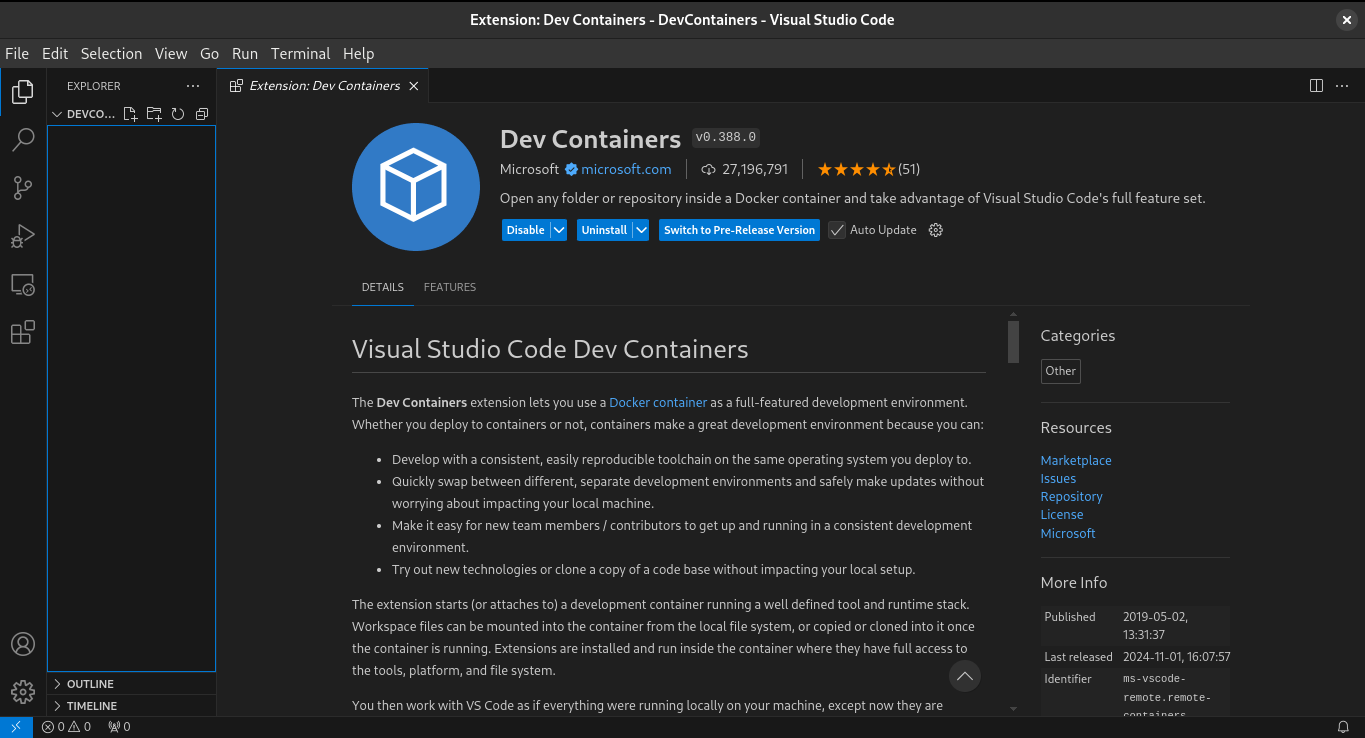
\includegraphics[keepaspectratio]{unidades/unidad4/./images/devContainer-extension.png}}

}

\caption{DevContainer en Visual Studio Code}

\end{figure}%

\section{Ejemplos:}\label{ejemplos-2}

En la parte inferior izquierda de Visual Studio Code existe un botón que
hace referencia a los \textbf{DevContainers}, al hacer clic en este
botón se abrirá un menú con las opciones para crear, abrir o configurar
un DevContainer.

En este punto damos clic en \textbf{New DevContainer} y seleccionamos la
opción \textbf{Python 3}. Esto creará un archivo \textbf{.devcontainer}
con la configuración necesaria para ejecutar la aplicación en un
contenedor Docker.

\begin{figure}[H]

{\centering \pandocbounded{\includegraphics[keepaspectratio]{unidades/unidad4/./images/new_DevContainer.png}}

}

\caption{New DevContainer}

\end{figure}%

En la imágen anterior podemos observar el menú de DevContainer, en esta
sección es posible seleccionar \textbf{New DevContainer}. Al seleccionar
esta opción se desplegará un menú con las opciones de configuración de
DevContainer.

\begin{figure}[H]

{\centering \pandocbounded{\includegraphics[keepaspectratio]{unidades/unidad4/./images/python3_DevContainer.png}}

}

\caption{Python 3 DevContainer}

\end{figure}%

En la imágen anterior se describe la búsqueda de diferentes plantillas,
en este caso seleccionamos \textbf{Python 3}. Al seleccionar esta opción
se creará un archivo \textbf{.devcontainer} con la configuración
necesaria para ejecutar la aplicación en un contenedor Docker.

\begin{figure}[H]

{\centering \pandocbounded{\includegraphics[keepaspectratio]{unidades/unidad4/./images/create_DevContainers.png}}

}

\caption{Create DevContainer}

\end{figure}%

Finalmente seleccoinamos la opción \textbf{Create DevContainers} para
crear el archivo \textbf{.devcontainer} con la configuración necesaria
para ejecutar la aplicación en un contenedor Docker.

\begin{figure}[H]

{\centering \pandocbounded{\includegraphics[keepaspectratio]{unidades/unidad4/./images/creando_DevContainer.png}}

}

\caption{Create DevContainer}

\end{figure}%

Ahora solo resta esperar como se observa en la imágen anterior la
creación del \textbf{DevContainer}. Una vez finalizado el proceso, se
abrirá una nueva ventana con el archivo \textbf{main.py} en el editor de
código y se mostrará un mensaje en la parte inferior derecha indicando
que se está construyendo el contenedor.

\begin{figure}[H]

{\centering \pandocbounded{\includegraphics[keepaspectratio]{unidades/unidad4/./images/python_in_DevContainer.png}}

}

\caption{Python in DevContainer}

\end{figure}%

Creamos una aplicación Hola Mundo en Python para ser ejecutada en un
DevContainer:

Crear un archivo \textbf{main.py} con el siguiente código:

\begin{Shaded}
\begin{Highlighting}[]
\CommentTok{\# main.py}
\BuiltInTok{print}\NormalTok{(}\StringTok{"Hola, Mundo!"}\NormalTok{)}
\end{Highlighting}
\end{Shaded}

Una vez creado el \textbf{DevContainer} se mostrará un mensaje en la
parte inferior derecha indicando que se está construyendo el contenedor.
En este punto se puede ejecutar la aplicación en el contenedor Docker
haciendo clic en el botón \textbf{Run} en la parte superior derecha.

Puedes verificar que la versión de python en el terminal del
DevContainer creado es diferente a la del Sistema Operativo en el que te
encuentres y la instalación global del sistema.

\section{Práctica}\label{pruxe1ctica-2}

\begin{itemize}
\item
  Crear un nuevo DevContainer con una plantilla en Python.
\item
  Crear un archivo \textbf{main.py} con un código sencillo en Python.
\item
  Ejecutar la aplicación en el DevContainer.
\end{itemize}

\section{Conclusiones}\label{conclusiones-6}

Los DevContainers son una herramienta poderosa para el desarrollo de
software, ya que permiten a los desarrolladores trabajar en un entorno
aislado y preconfigurado, sin tener que preocuparse por la configuración
del sistema operativo, las dependencias de software o las bibliotecas de
terceros. Los DevContainers proporcionan un entorno de desarrollo
consistente y reproducible, lo que garantiza que las aplicaciones se
ejecuten de la misma manera en diferentes entornos.

\part{Unidad 5: Python Avanzado}

\chapter{Conceptos Avanzados en
Python}\label{conceptos-avanzados-en-python}

En este capitulo en particular aprenderemos los conceptos avanzados que
necesitamos conocer de Python para poder avanzar con temas relacionados
al desarrollo de software.

En el mismo aprenderemos:

\begin{enumerate}
\def\labelenumi{\arabic{enumi}.}
\item
  \href{./1_exepciones_manejo_de_errores.qmd}{Exepciones y Manejo de
  Errores}
\item
  \href{./2_lectura_y_escritura_de_archivos.qmd}{Lectura y Escritura de
  Archivos}
\item
  \href{./3_programacion_funcional.qmd}{Programación Funcional}
\item
  \href{./4_comprension_y_generadores.qmd}{Comprención y Generadores}
\item
  \href{./5_modulos_y_paquetes_avanzados.qmd}{Módulos y Paquetes}
\item
  \href{./6_decoradores_y_context_managers.qmd}{Decoradores y Context
  Managers}
\item
  \href{./7_colecciones_de_datos_y_estructuras_especializadas.qmd}{Colecciones
  de Datos y Estructuras Especializadas}
\item
  \href{./8_manipulacion_de_fechas_y_tiempos.qmd}{Manipulación de Fechas
  y Tiempos}
\item
  \href{./9_concurrencia_y_paralelismo.qmd}{Concurrencia y Paralelismo}
\item
  \href{./10_pruebas_y_debugging.qmd}{Pruebas y Debugging}
\end{enumerate}

Este capítulo cubre varios de los aspectos más avanzados de Python, y
proporciona una base sólida para desarrollar aplicaciones web fullstack
más complejas. Los ejemplos prácticos te ayudarán a entender cómo
aplicar estos conceptos en situaciones reales.

\chapter{Excepciones y Manejo de
Errores}\label{excepciones-y-manejo-de-errores}

\begin{figure}[H]

{\centering \pandocbounded{\includegraphics[keepaspectratio]{unidades/unidad5/./images/exepciones.png}}

}

\caption{Excepciones y Manejo de Errores}

\end{figure}%

El manejo adecuado de errores es esencial para escribir código robusto.
Las excepciones permiten manejar situaciones inesperadas durante la
ejecución de un programa sin que este termine abruptamente.

\subsection{Conceptos clave}\label{conceptos-clave}

\begin{itemize}
\tightlist
\item
  \textbf{try}: Bloque donde intentamos ejecutar código que puede
  generar una excepción.
\item
  \textbf{except}: Bloque donde capturamos y gestionamos una excepción.
\item
  \textbf{else}: Bloque que se ejecuta si no hay excepciones.
\item
  \textbf{finally}: Bloque que se ejecuta independientemente de si hubo
  una excepción o no.
\end{itemize}

\subsection{Ejemplo}\label{ejemplo}

\begin{Shaded}
\begin{Highlighting}[]
\ControlFlowTok{try}\NormalTok{:}
\NormalTok{    numero }\OperatorTok{=} \BuiltInTok{int}\NormalTok{(}\BuiltInTok{input}\NormalTok{(}\StringTok{"Introduce un número: "}\NormalTok{))}
\ControlFlowTok{except} \PreprocessorTok{ValueError} \ImportTok{as}\NormalTok{ e:}
    \BuiltInTok{print}\NormalTok{(}\SpecialStringTok{f"Error: }\SpecialCharTok{\{}\NormalTok{e}\SpecialCharTok{\}}\SpecialStringTok{. Introduce un número válido."}\NormalTok{)}
\ControlFlowTok{else}\NormalTok{:}
    \BuiltInTok{print}\NormalTok{(}\SpecialStringTok{f"El número es }\SpecialCharTok{\{}\NormalTok{numero}\SpecialCharTok{\}}\SpecialStringTok{."}\NormalTok{)}
\ControlFlowTok{finally}\NormalTok{:}
    \BuiltInTok{print}\NormalTok{(}\StringTok{"Operación terminada."}\NormalTok{)}
\end{Highlighting}
\end{Shaded}

\subsection{Excepciones
personalizadas}\label{excepciones-personalizadas}

Podemos crear nuestras propias excepciones para situaciones específicas.

\begin{Shaded}
\begin{Highlighting}[]
\KeywordTok{class}\NormalTok{ MiError(}\PreprocessorTok{Exception}\NormalTok{):}
    \KeywordTok{def} \FunctionTok{\_\_init\_\_}\NormalTok{(}\VariableTok{self}\NormalTok{, mensaje):}
        \VariableTok{self}\NormalTok{.mensaje }\OperatorTok{=}\NormalTok{ mensaje}
        \BuiltInTok{super}\NormalTok{().}\FunctionTok{\_\_init\_\_}\NormalTok{(}\VariableTok{self}\NormalTok{.mensaje)}

\ControlFlowTok{try}\NormalTok{:}
    \ControlFlowTok{raise}\NormalTok{ MiError(}\StringTok{"Algo salió mal"}\NormalTok{)}
\ControlFlowTok{except}\NormalTok{ MiError }\ImportTok{as}\NormalTok{ e:}
    \BuiltInTok{print}\NormalTok{(}\SpecialStringTok{f"Capturado: }\SpecialCharTok{\{}\NormalTok{e}\SpecialCharTok{\}}\SpecialStringTok{"}\NormalTok{)}
\end{Highlighting}
\end{Shaded}

\subsection{Ejemplo Práctico}\label{ejemplo-pruxe1ctico-1}

\textbf{Objetivo}:

Aprender a manejar excepciones en Python para crear un programa robusto
que gestione entradas de usuario incorrectas.

\textbf{Descripción}: Crear un programa que pida al usuario un número, y
en caso de que se ingrese algo que no sea un número, maneje el error de
manera adecuada, mostrando un mensaje informativo.

\textbf{Instrucciones}:

\begin{itemize}
\item
  Utiliza un bloque try-except para manejar excepciones de tipo
  ValueError.
\item
  Agrega un bloque else para confirmar la entrada del usuario si es
  válida.
\item
  Incluye un bloque finally que imprima un mensaje de despedida.
\end{itemize}

Posibles soluciones

\textbf{Código}:

\begin{Shaded}
\begin{Highlighting}[]
\KeywordTok{def}\NormalTok{ pedir\_numero():}
    \ControlFlowTok{try}\NormalTok{:}
\NormalTok{        numero }\OperatorTok{=} \BuiltInTok{int}\NormalTok{(}\BuiltInTok{input}\NormalTok{(}\StringTok{"Introduce un número: "}\NormalTok{))}
    \ControlFlowTok{except} \PreprocessorTok{ValueError}\NormalTok{:}
        \BuiltInTok{print}\NormalTok{(}\StringTok{"¡Error! No has introducido un número válido."}\NormalTok{)}
    \ControlFlowTok{else}\NormalTok{:}
        \BuiltInTok{print}\NormalTok{(}\SpecialStringTok{f"Has introducido el número: }\SpecialCharTok{\{}\NormalTok{numero}\SpecialCharTok{\}}\SpecialStringTok{"}\NormalTok{)}
    \ControlFlowTok{finally}\NormalTok{:}
        \BuiltInTok{print}\NormalTok{(}\StringTok{"Fin del programa"}\NormalTok{)}

\NormalTok{pedir\_numero()}
\end{Highlighting}
\end{Shaded}

\chapter{Lectura y Escritura de
Archivos}\label{lectura-y-escritura-de-archivos}

\begin{figure}[H]

{\centering \pandocbounded{\includegraphics[keepaspectratio]{unidades/unidad5/./images/archivos.png}}

}

\caption{Lectura y Escritura de Archivos}

\end{figure}%

Leer y escribir archivos es una habilidad básica en el desarrollo de
aplicaciones, como para guardar configuraciones o almacenar datos de
usuarios.

\subsection{Conceptos clave}\label{conceptos-clave-1}

\begin{itemize}
\item
  \textbf{open}: Función para abrir archivos.
\item
  \textbf{Modos de apertura}:

  \begin{itemize}
  \item
    \textbf{`r'}: Lectura.
  \item
    \textbf{`w'}: Escritura.
  \item
    \textbf{`a'}: Añadir datos.
  \end{itemize}
\end{itemize}

\textbf{El contexto with}: Manejo automático de recursos.

Ejemplo

\begin{Shaded}
\begin{Highlighting}[]
\CommentTok{\# Escritura en archivo}
\ControlFlowTok{with} \BuiltInTok{open}\NormalTok{(}\StringTok{\textquotesingle{}archivo.txt\textquotesingle{}}\NormalTok{, }\StringTok{\textquotesingle{}w\textquotesingle{}}\NormalTok{) }\ImportTok{as}\NormalTok{ f:}
\NormalTok{    f.write(}\StringTok{"Hola, Mundo!}\CharTok{\textbackslash{}n}\StringTok{"}\NormalTok{)}

\CommentTok{\# Lectura de archivo}
\ControlFlowTok{with} \BuiltInTok{open}\NormalTok{(}\StringTok{\textquotesingle{}archivo.txt\textquotesingle{}}\NormalTok{, }\StringTok{\textquotesingle{}r\textquotesingle{}}\NormalTok{) }\ImportTok{as}\NormalTok{ f:}
\NormalTok{    contenido }\OperatorTok{=}\NormalTok{ f.read()}
    \BuiltInTok{print}\NormalTok{(contenido)}
\end{Highlighting}
\end{Shaded}

\subsection{Archivos binarios}\label{archivos-binarios}

Podemos manejar archivos binarios usando el modo \textbf{`rb'} o
\textbf{`wb'}:

\begin{Shaded}
\begin{Highlighting}[]
\CommentTok{\# Lectura binaria}
\ControlFlowTok{with} \BuiltInTok{open}\NormalTok{(}\StringTok{\textquotesingle{}imagen.jpg\textquotesingle{}}\NormalTok{, }\StringTok{\textquotesingle{}rb\textquotesingle{}}\NormalTok{) }\ImportTok{as}\NormalTok{ f:}
\NormalTok{    datos }\OperatorTok{=}\NormalTok{ f.read()}
\end{Highlighting}
\end{Shaded}

\subsection{Ejemplo Práctico}\label{ejemplo-pruxe1ctico-2}

\textbf{Objetivo}:

Aprender a leer y escribir archivos de texto en Python.

\textbf{Descripción}: Crear un programa que pida al usuario un texto y
lo escriba en un archivo de texto. Luego, el programa debe leer el
archivo y mostrar su contenido.

\textbf{Instrucciones}:

\begin{itemize}
\item
  Pide un texto al usuario.
\item
  Escribe ese texto en un archivo llamado entrada.txt.
\item
  Luego, lee el archivo y muestra su contenido en la consola.
\end{itemize}

Posibles soluciones

\textbf{Código}:

\begin{Shaded}
\begin{Highlighting}[]
\KeywordTok{def}\NormalTok{ escribir\_y\_leer\_archivo():}
    \CommentTok{\# Escribir en el archivo}
    \ControlFlowTok{with} \BuiltInTok{open}\NormalTok{(}\StringTok{\textquotesingle{}entrada.txt\textquotesingle{}}\NormalTok{, }\StringTok{\textquotesingle{}w\textquotesingle{}}\NormalTok{) }\ImportTok{as}\NormalTok{ archivo:}
\NormalTok{        texto }\OperatorTok{=} \BuiltInTok{input}\NormalTok{(}\StringTok{"Escribe algo: "}\NormalTok{)}
\NormalTok{        archivo.write(texto)}
    
    \CommentTok{\# Leer el archivo}
    \ControlFlowTok{with} \BuiltInTok{open}\NormalTok{(}\StringTok{\textquotesingle{}entrada.txt\textquotesingle{}}\NormalTok{, }\StringTok{\textquotesingle{}r\textquotesingle{}}\NormalTok{) }\ImportTok{as}\NormalTok{ archivo:}
\NormalTok{        contenido }\OperatorTok{=}\NormalTok{ archivo.read()}
        \BuiltInTok{print}\NormalTok{(}\SpecialStringTok{f"Contenido del archivo: }\SpecialCharTok{\{}\NormalTok{contenido}\SpecialCharTok{\}}\SpecialStringTok{"}\NormalTok{)}

\NormalTok{escribir\_y\_leer\_archivo()}
\end{Highlighting}
\end{Shaded}

:::

\chapter{Programación Funcional}\label{programaciuxf3n-funcional}

\begin{figure}[H]

{\centering \pandocbounded{\includegraphics[keepaspectratio]{unidades/unidad5/./images/funciones.png}}

}

\caption{Programación Funcional}

\end{figure}%

Python soporta parcialmente la programación funcional, lo que permite
escribir código más limpio y conciso.

\subsection{Conceptos clave}\label{conceptos-clave-2}

\begin{itemize}
\item
  \textbf{lambda}: Funciones anónimas.
\item
  \textbf{map}: Aplica una función a cada ítem de un iterable.
\item
  \textbf{filter}: Filtra elementos de un iterable según una condición.
\item
  \textbf{reduce}: Reducción de un iterable a un único valor.
\end{itemize}

\subsection{Comprensión de listas y
generadores.}\label{comprensiuxf3n-de-listas-y-generadores.}

Ejemplo

\begin{Shaded}
\begin{Highlighting}[]
\CommentTok{\# Uso de lambda y map}
\NormalTok{numeros }\OperatorTok{=}\NormalTok{ [}\DecValTok{1}\NormalTok{, }\DecValTok{2}\NormalTok{, }\DecValTok{3}\NormalTok{, }\DecValTok{4}\NormalTok{]}
\NormalTok{dobles }\OperatorTok{=} \BuiltInTok{list}\NormalTok{(}\BuiltInTok{map}\NormalTok{(}\KeywordTok{lambda}\NormalTok{ x: x }\OperatorTok{*} \DecValTok{2}\NormalTok{, numeros))}
\BuiltInTok{print}\NormalTok{(dobles)}

\CommentTok{\# Uso de filter}
\NormalTok{pares }\OperatorTok{=} \BuiltInTok{list}\NormalTok{(}\BuiltInTok{filter}\NormalTok{(}\KeywordTok{lambda}\NormalTok{ x: x }\OperatorTok{\%} \DecValTok{2} \OperatorTok{==} \DecValTok{0}\NormalTok{, numeros))}
\BuiltInTok{print}\NormalTok{(pares)}

\CommentTok{\# Uso de reduce}
\ImportTok{from}\NormalTok{ functools }\ImportTok{import} \BuiltInTok{reduce}
\NormalTok{suma }\OperatorTok{=} \BuiltInTok{reduce}\NormalTok{(}\KeywordTok{lambda}\NormalTok{ x, y: x }\OperatorTok{+}\NormalTok{ y, numeros)}
\BuiltInTok{print}\NormalTok{(suma)}
\end{Highlighting}
\end{Shaded}

\subsection{Ejemplo Práctico}\label{ejemplo-pruxe1ctico-3}

\textbf{Objetivo}:

Aprender a utilizar funciones lambda y operaciones como map, filter y
reduce para trabajar con colecciones de datos.

\textbf{Descripción}:

Crear un programa que utilice una lista de números para aplicar
operaciones funcionales usando lambda, map, filter y reduce.

\textbf{Instrucciones}:

\begin{itemize}
\item
  Crea una lista de números del 1 al 10.
\item
  Usa map con una función lambda para obtener el doble de cada número.
\item
  Usa filter para filtrar solo los números pares.
\item
  Usa reduce para obtener la suma de todos los números en la lista.
\end{itemize}

Posibles soluciones

\textbf{Código}:

\begin{Shaded}
\begin{Highlighting}[]
\ImportTok{from}\NormalTok{ functools }\ImportTok{import} \BuiltInTok{reduce}

\CommentTok{\# Lista de números}
\NormalTok{numeros }\OperatorTok{=}\NormalTok{ [}\DecValTok{1}\NormalTok{, }\DecValTok{2}\NormalTok{, }\DecValTok{3}\NormalTok{, }\DecValTok{4}\NormalTok{, }\DecValTok{5}\NormalTok{, }\DecValTok{6}\NormalTok{, }\DecValTok{7}\NormalTok{, }\DecValTok{8}\NormalTok{, }\DecValTok{9}\NormalTok{, }\DecValTok{10}\NormalTok{]}

\CommentTok{\# Usando map con lambda}
\NormalTok{dobles }\OperatorTok{=} \BuiltInTok{list}\NormalTok{(}\BuiltInTok{map}\NormalTok{(}\KeywordTok{lambda}\NormalTok{ x: x }\OperatorTok{*} \DecValTok{2}\NormalTok{, numeros))}
\BuiltInTok{print}\NormalTok{(}\SpecialStringTok{f"Lista de dobles: }\SpecialCharTok{\{}\NormalTok{dobles}\SpecialCharTok{\}}\SpecialStringTok{"}\NormalTok{)}

\CommentTok{\# Usando filter con lambda}
\NormalTok{pares }\OperatorTok{=} \BuiltInTok{list}\NormalTok{(}\BuiltInTok{filter}\NormalTok{(}\KeywordTok{lambda}\NormalTok{ x: x }\OperatorTok{\%} \DecValTok{2} \OperatorTok{==} \DecValTok{0}\NormalTok{, numeros))}
\BuiltInTok{print}\NormalTok{(}\SpecialStringTok{f"Números pares: }\SpecialCharTok{\{}\NormalTok{pares}\SpecialCharTok{\}}\SpecialStringTok{"}\NormalTok{)}

\CommentTok{\# Usando reduce con lambda}
\NormalTok{suma }\OperatorTok{=} \BuiltInTok{reduce}\NormalTok{(}\KeywordTok{lambda}\NormalTok{ x, y: x }\OperatorTok{+}\NormalTok{ y, numeros)}
\BuiltInTok{print}\NormalTok{(}\SpecialStringTok{f"Suma de números: }\SpecialCharTok{\{}\NormalTok{suma}\SpecialCharTok{\}}\SpecialStringTok{"}\NormalTok{)}
\end{Highlighting}
\end{Shaded}

\chapter{Comprensiones y Generadores}\label{comprensiones-y-generadores}

\begin{figure}[H]

{\centering \pandocbounded{\includegraphics[keepaspectratio]{unidades/unidad5/./images/comprensiones_y_generadores.png}}

}

\caption{Comprensiones y Generadores}

\end{figure}%

Las comprensiones proporcionan una manera más compacta de crear
colecciones. Los generadores permiten trabajar con grandes volúmenes de
datos de manera eficiente.

\subsection{Conceptos clave}\label{conceptos-clave-3}

\begin{itemize}
\item
  Comprensión de listas, diccionarios y conjuntos.
\item
  Generadores y yield.
\end{itemize}

Ejemplo

\begin{Shaded}
\begin{Highlighting}[]
\CommentTok{\# Comprensión de lista}
\NormalTok{cuadrados }\OperatorTok{=}\NormalTok{ [x}\OperatorTok{**}\DecValTok{2} \ControlFlowTok{for}\NormalTok{ x }\KeywordTok{in} \BuiltInTok{range}\NormalTok{(}\DecValTok{5}\NormalTok{)]}
\BuiltInTok{print}\NormalTok{(cuadrados)}

\CommentTok{\# Generador}
\KeywordTok{def}\NormalTok{ contador():}
    \ControlFlowTok{for}\NormalTok{ i }\KeywordTok{in} \BuiltInTok{range}\NormalTok{(}\DecValTok{5}\NormalTok{):}
        \ControlFlowTok{yield}\NormalTok{ i}

\NormalTok{gen }\OperatorTok{=}\NormalTok{ contador()}
\ControlFlowTok{for}\NormalTok{ valor }\KeywordTok{in}\NormalTok{ gen:}
    \BuiltInTok{print}\NormalTok{(valor)}
\end{Highlighting}
\end{Shaded}

\subsection{Ejemplo Práctico}\label{ejemplo-pruxe1ctico-4}

\textbf{Objetivo}:

Aprender a crear listas, diccionarios y generadores utilizando
comprensiones y el comando yield.

\textbf{Descripción}:

Crea un programa que use comprensiones de listas y diccionarios para
realizar operaciones sobre una lista de palabras, y usa un generador
para crear una secuencia de números.

\textbf{Instrucciones}:

\begin{itemize}
\item
  Usa una comprensión de lista para crear una lista de las longitudes de
  las palabras.
\item
  Usa una comprensión de diccionario para contar la frecuencia de cada
  letra en un conjunto de palabras.
\item
  Usa un generador para producir los primeros 10 números pares.
\end{itemize}

Posibles soluciones

\textbf{Código}:

\begin{Shaded}
\begin{Highlighting}[]
\CommentTok{\# Lista de palabras}
\NormalTok{palabras }\OperatorTok{=}\NormalTok{ [}\StringTok{"python"}\NormalTok{, }\StringTok{"django"}\NormalTok{, }\StringTok{"flask"}\NormalTok{, }\StringTok{"javascript"}\NormalTok{]}

\CommentTok{\# Comprensión de lista para obtener las longitudes de las palabras}
\NormalTok{longitudes }\OperatorTok{=}\NormalTok{ [}\BuiltInTok{len}\NormalTok{(palabra) }\ControlFlowTok{for}\NormalTok{ palabra }\KeywordTok{in}\NormalTok{ palabras]}
\BuiltInTok{print}\NormalTok{(}\SpecialStringTok{f"Longitudes de las palabras: }\SpecialCharTok{\{}\NormalTok{longitudes}\SpecialCharTok{\}}\SpecialStringTok{"}\NormalTok{)}

\CommentTok{\# Comprensión de diccionario para contar las frecuencias de las letras}
\NormalTok{frecuencia }\OperatorTok{=}\NormalTok{ \{letra: palabras[}\DecValTok{0}\NormalTok{].count(letra) }\ControlFlowTok{for}\NormalTok{ letra }\KeywordTok{in}\NormalTok{ palabras[}\DecValTok{0}\NormalTok{]\}}
\BuiltInTok{print}\NormalTok{(}\SpecialStringTok{f"Frecuencia de letras en la primera palabra: }\SpecialCharTok{\{}\NormalTok{frecuencia}\SpecialCharTok{\}}\SpecialStringTok{"}\NormalTok{)}

\CommentTok{\# Generador para números pares}
\KeywordTok{def}\NormalTok{ generador\_pares():}
    \ControlFlowTok{for}\NormalTok{ i }\KeywordTok{in} \BuiltInTok{range}\NormalTok{(}\DecValTok{0}\NormalTok{, }\DecValTok{20}\NormalTok{, }\DecValTok{2}\NormalTok{):}
        \ControlFlowTok{yield}\NormalTok{ i}

\CommentTok{\# Mostrar los números generados}
\ControlFlowTok{for}\NormalTok{ numero }\KeywordTok{in}\NormalTok{ generador\_pares():}
    \BuiltInTok{print}\NormalTok{(numero)}
\end{Highlighting}
\end{Shaded}

\chapter{Módulos y Paquetes
Avanzados}\label{muxf3dulos-y-paquetes-avanzados}

\begin{figure}[H]

{\centering \pandocbounded{\includegraphics[keepaspectratio]{unidades/unidad5/./images/modulos_y_paquetes.png}}

}

\caption{Módulos y Paquetes}

\end{figure}%

Organizar el código en módulos y paquetes es fundamental para proyectos
grandes.

\subsection{Conceptos clave}\label{conceptos-clave-4}

\begin{itemize}
\item
  Importación relativa y absoluta.
\item
  \textbf{\textbf{init}.py}: Archivo necesario para que un directorio
  sea reconocido como un paquete.
\item
  Gestión de dependencias.
\end{itemize}

Ejemplo

\begin{Shaded}
\begin{Highlighting}[]
\CommentTok{\# Importación absoluta}
\ImportTok{import}\NormalTok{ mi\_modulo}

\CommentTok{\# Importación relativa}
\ImportTok{from}\NormalTok{ . }\ImportTok{import}\NormalTok{ mi\_modulo}
\end{Highlighting}
\end{Shaded}

\subsection{Ejemplo Práctico}\label{ejemplo-pruxe1ctico-5}

\textbf{Objetivo}:

Aprender a organizar el código en módulos y paquetes para proyectos más
grandes.

\textbf{Descripción}:

Crea un proyecto con múltiples archivos Python y organiza el código en
módulos. Simula un programa de gestión de tareas.

\textbf{Instrucciones}:

\begin{itemize}
\item
  Crea una carpeta llamada tareas.
\item
  Dentro de esa carpeta, crea tres archivos:
\item
  \textbf{init}.py: Para inicializar el paquete.
\item
  gestor.py: Para gestionar tareas.
\item
  principal.py: Para ejecutar el programa.
\end{itemize}

Posibles soluciones

\textbf{Código}:

\textbf{gestor.py}:

\begin{Shaded}
\begin{Highlighting}[]
\KeywordTok{def}\NormalTok{ agregar\_tarea(tarea):}
\NormalTok{    tareas.append(tarea)}
    \BuiltInTok{print}\NormalTok{(}\SpecialStringTok{f"Tarea \textquotesingle{}}\SpecialCharTok{\{}\NormalTok{tarea}\SpecialCharTok{\}}\SpecialStringTok{\textquotesingle{} agregada."}\NormalTok{)}
    
\KeywordTok{def}\NormalTok{ listar\_tareas():}
    \ControlFlowTok{for}\NormalTok{ tarea }\KeywordTok{in}\NormalTok{ tareas:}
        \BuiltInTok{print}\NormalTok{(}\SpecialStringTok{f"{-} }\SpecialCharTok{\{}\NormalTok{tarea}\SpecialCharTok{\}}\SpecialStringTok{"}\NormalTok{)}

\NormalTok{tareas }\OperatorTok{=}\NormalTok{ []}
\end{Highlighting}
\end{Shaded}

\textbf{principal.py}:

\begin{Shaded}
\begin{Highlighting}[]
\ImportTok{from}\NormalTok{ tareas.gestor }\ImportTok{import}\NormalTok{ agregar\_tarea, listar\_tareas}

\NormalTok{agregar\_tarea(}\StringTok{"Estudiar Python"}\NormalTok{)}
\NormalTok{agregar\_tarea(}\StringTok{"Leer libro de programación"}\NormalTok{)}
\NormalTok{listar\_tareas()}
\end{Highlighting}
\end{Shaded}

\chapter{Decoradores y Context
Managers}\label{decoradores-y-context-managers}

\begin{figure}[H]

{\centering \pandocbounded{\includegraphics[keepaspectratio]{unidades/unidad5/./images/decoradores.png}}

}

\caption{Decoradores}

\end{figure}%

Los decoradores permiten modificar el comportamiento de una función,
mientras que los context managers gestionan recursos como archivos o
conexiones a bases de datos.

\subsection{Conceptos clave}\label{conceptos-clave-5}

\begin{itemize}
\item
  \textbf{(\textbf{decorator?})}: Sintaxis para aplicar un decorador.
\item
  \textbf{with y \textbf{enter}, \textbf{exit}}: Para crear context
  managers.
\end{itemize}

Ejemplo

\begin{Shaded}
\begin{Highlighting}[]
\CommentTok{\# Decorador}
\KeywordTok{def}\NormalTok{ mi\_decorador(func):}
    \KeywordTok{def}\NormalTok{ wrapper():}
        \BuiltInTok{print}\NormalTok{(}\StringTok{"Antes de la función"}\NormalTok{)}
\NormalTok{        func()}
        \BuiltInTok{print}\NormalTok{(}\StringTok{"Después de la función"}\NormalTok{)}
    \ControlFlowTok{return}\NormalTok{ wrapper}

\AttributeTok{@mi\_decorador}
\KeywordTok{def}\NormalTok{ saludo():}
    \BuiltInTok{print}\NormalTok{(}\StringTok{"Hola"}\NormalTok{)}

\NormalTok{saludo()}

\CommentTok{\# Context manager}
\KeywordTok{class}\NormalTok{ MiContexto:}
    \KeywordTok{def} \FunctionTok{\_\_enter\_\_}\NormalTok{(}\VariableTok{self}\NormalTok{):}
        \BuiltInTok{print}\NormalTok{(}\StringTok{"Entrando al contexto"}\NormalTok{)}
        \ControlFlowTok{return} \VariableTok{self}

    \KeywordTok{def} \FunctionTok{\_\_exit\_\_}\NormalTok{(}\VariableTok{self}\NormalTok{, exc\_type, exc\_value, traceback):}
        \BuiltInTok{print}\NormalTok{(}\StringTok{"Saliendo del contexto"}\NormalTok{)}

\ControlFlowTok{with}\NormalTok{ MiContexto():}
    \BuiltInTok{print}\NormalTok{(}\StringTok{"Dentro del contexto"}\NormalTok{)}
\end{Highlighting}
\end{Shaded}

\subsection{Ejemplo Práctico}\label{ejemplo-pruxe1ctico-6}

\textbf{Objetivo}:

Aprender a crear decoradores y context managers en Python.

\textbf{Descripción}: Crea un decorador que registre la ejecución de una
función y un context manager que gestione un archivo de log.

\textbf{Instrucciones}:

\begin{itemize}
\item
  Crea un decorador que imprima la fecha y hora de la ejecución de una
  función.
\item
  Crea un context manager que gestione la apertura y cierre de un
  archivo de log.
\end{itemize}

Posibles soluciones

\textbf{Código}:

\begin{Shaded}
\begin{Highlighting}[]
\ImportTok{import}\NormalTok{ time}

\CommentTok{\# Decorador que registra la ejecución de una función}
\KeywordTok{def}\NormalTok{ registrar(func):}
    \KeywordTok{def}\NormalTok{ wrapper(}\OperatorTok{*}\NormalTok{args, }\OperatorTok{**}\NormalTok{kwargs):}
        \BuiltInTok{print}\NormalTok{(}\SpecialStringTok{f"Ejecutando }\SpecialCharTok{\{}\NormalTok{func}\SpecialCharTok{.}\VariableTok{\_\_name\_\_}\SpecialCharTok{\}}\SpecialStringTok{ a las }\SpecialCharTok{\{}\NormalTok{time}\SpecialCharTok{.}\NormalTok{strftime(}\StringTok{\textquotesingle{}\%H:\%M:\%S\textquotesingle{}}\NormalTok{)}\SpecialCharTok{\}}\SpecialStringTok{"}\NormalTok{)}
        \ControlFlowTok{return}\NormalTok{ func(}\OperatorTok{*}\NormalTok{args, }\OperatorTok{**}\NormalTok{kwargs)}
    \ControlFlowTok{return}\NormalTok{ wrapper}

\AttributeTok{@registrar}
\KeywordTok{def}\NormalTok{ saludo():}
    \BuiltInTok{print}\NormalTok{(}\StringTok{"¡Hola, Mundo!"}\NormalTok{)}

\NormalTok{saludo()}

\CommentTok{\# Context manager para log}
\KeywordTok{class}\NormalTok{ LogManager:}
    \KeywordTok{def} \FunctionTok{\_\_enter\_\_}\NormalTok{(}\VariableTok{self}\NormalTok{):}
        \VariableTok{self}\NormalTok{.archivo }\OperatorTok{=} \BuiltInTok{open}\NormalTok{(}\StringTok{\textquotesingle{}log.txt\textquotesingle{}}\NormalTok{, }\StringTok{\textquotesingle{}a\textquotesingle{}}\NormalTok{)}
        \ControlFlowTok{return} \VariableTok{self}\NormalTok{.archivo}

    \KeywordTok{def} \FunctionTok{\_\_exit\_\_}\NormalTok{(}\VariableTok{self}\NormalTok{, exc\_type, exc\_value, traceback):}
        \VariableTok{self}\NormalTok{.archivo.close()}

\ControlFlowTok{with}\NormalTok{ LogManager() }\ImportTok{as}\NormalTok{ log:}
\NormalTok{    log.write(}\SpecialStringTok{f"Acción registrada a las }\SpecialCharTok{\{}\NormalTok{time}\SpecialCharTok{.}\NormalTok{strftime(}\StringTok{\textquotesingle{}\%H:\%M:\%S\textquotesingle{}}\NormalTok{)}\SpecialCharTok{\}}\CharTok{\textbackslash{}n}\SpecialStringTok{"}\NormalTok{)}
\end{Highlighting}
\end{Shaded}

\chapter{Colecciones de Datos y Estructuras
Especializadas}\label{colecciones-de-datos-y-estructuras-especializadas}

\begin{figure}[H]

{\centering \pandocbounded{\includegraphics[keepaspectratio]{unidades/unidad5/./images/colecciones.png}}

}

\caption{Colecciones}

\end{figure}%

La librería collections ofrece estructuras de datos útiles para
optimizar el código.

\subsection{Conceptos clave}\label{conceptos-clave-6}

\begin{itemize}
\item
  \textbf{Counter}: Cuenta elementos.
\item
  \textbf{deque}: Cola de doble extremo.
\item
  \textbf{defaultdict}: Diccionario con valores predeterminados.
\item
  \textbf{namedtuple}: Tupla con nombre.
\end{itemize}

Ejemplo

\begin{Shaded}
\begin{Highlighting}[]
\ImportTok{from}\NormalTok{ collections }\ImportTok{import}\NormalTok{ Counter, deque, defaultdict, namedtuple}

\CommentTok{\# Counter}
\NormalTok{c }\OperatorTok{=}\NormalTok{ Counter([}\DecValTok{1}\NormalTok{, }\DecValTok{2}\NormalTok{, }\DecValTok{2}\NormalTok{, }\DecValTok{3}\NormalTok{])}
\BuiltInTok{print}\NormalTok{(c)}

\CommentTok{\# deque}
\NormalTok{d }\OperatorTok{=}\NormalTok{ deque([}\DecValTok{1}\NormalTok{, }\DecValTok{2}\NormalTok{, }\DecValTok{3}\NormalTok{])}
\NormalTok{d.append(}\DecValTok{4}\NormalTok{)}
\BuiltInTok{print}\NormalTok{(d)}

\CommentTok{\# defaultdict}
\NormalTok{dd }\OperatorTok{=}\NormalTok{ defaultdict(}\BuiltInTok{int}\NormalTok{)}
\NormalTok{dd[}\StringTok{\textquotesingle{}a\textquotesingle{}}\NormalTok{] }\OperatorTok{+=} \DecValTok{1}
\BuiltInTok{print}\NormalTok{(dd)}

\CommentTok{\# namedtuple}
\NormalTok{Persona }\OperatorTok{=}\NormalTok{ namedtuple(}\StringTok{\textquotesingle{}Persona\textquotesingle{}}\NormalTok{, }\StringTok{\textquotesingle{}nombre edad\textquotesingle{}}\NormalTok{)}
\NormalTok{persona }\OperatorTok{=}\NormalTok{ Persona(nombre}\OperatorTok{=}\StringTok{\textquotesingle{}Juan\textquotesingle{}}\NormalTok{, edad}\OperatorTok{=}\DecValTok{30}\NormalTok{)}
\BuiltInTok{print}\NormalTok{(persona.nombre)}
\end{Highlighting}
\end{Shaded}

\subsection{Ejemplo Práctico}\label{ejemplo-pruxe1ctico-7}

\textbf{Objetivo}:

Aprender a utilizar estructuras de datos avanzadas como Counter, deque y
defaultdict.

\textbf{Descripción}:

Crea un programa que utilice Counter para contar elementos, deque para
manipular una cola y defaultdict para un diccionario con valores
predeterminados.

\textbf{Instrucciones}:

\begin{itemize}
\item
  Usa Counter para contar las palabras en una frase.
\item
  Usa deque para simular una cola.
\item
  Usa defaultdict para contar ocurrencias de letras en un texto.
\end{itemize}

Posibles soluciones

\textbf{Código}:

\begin{Shaded}
\begin{Highlighting}[]
\ImportTok{from}\NormalTok{ collections }\ImportTok{import}\NormalTok{ Counter, deque, defaultdict}

\CommentTok{\# Usando Counter}
\NormalTok{frase }\OperatorTok{=} \StringTok{"python python flask flask flask"}
\NormalTok{contador }\OperatorTok{=}\NormalTok{ Counter(frase.split())}
\BuiltInTok{print}\NormalTok{(contador)}

\CommentTok{\# Usando deque}
\NormalTok{cola }\OperatorTok{=}\NormalTok{ deque([}\DecValTok{1}\NormalTok{, }\DecValTok{2}\NormalTok{, }\DecValTok{3}\NormalTok{])}
\NormalTok{cola.append(}\DecValTok{4}\NormalTok{)}
\NormalTok{cola.popleft()}
\BuiltInTok{print}\NormalTok{(cola)}

\CommentTok{\# Usando defaultdict}
\NormalTok{texto }\OperatorTok{=} \StringTok{"hola mundo"}
\NormalTok{letras }\OperatorTok{=}\NormalTok{ defaultdict(}\BuiltInTok{int}\NormalTok{)}
\ControlFlowTok{for}\NormalTok{ letra }\KeywordTok{in}\NormalTok{ texto:}
\NormalTok{    letras[letra] }\OperatorTok{+=} \DecValTok{1}
\BuiltInTok{print}\NormalTok{(letras)}
\end{Highlighting}
\end{Shaded}

\chapter{Manipulación de Fechas y
Tiempos}\label{manipulaciuxf3n-de-fechas-y-tiempos}

\begin{figure}[H]

{\centering \pandocbounded{\includegraphics[keepaspectratio]{unidades/unidad5/./images/fechas.png}}

}

\caption{Fechas}

\end{figure}%

Trabajar con fechas y horas es una parte fundamental en muchas
aplicaciones.

\subsection{Conceptos clave}\label{conceptos-clave-7}

\begin{itemize}
\item
  \textbf{datetime}: Para trabajar con fechas y horas.
\item
  \textbf{time}: Para trabajar con tiempos.
\item
  \textbf{pytz}: Para manejar zonas horarias.
\end{itemize}

Ejemplo

\begin{Shaded}
\begin{Highlighting}[]
\ImportTok{from}\NormalTok{ datetime }\ImportTok{import}\NormalTok{ datetime}

\CommentTok{\# Fecha y hora actuales}
\NormalTok{ahora }\OperatorTok{=}\NormalTok{ datetime.now()}
\BuiltInTok{print}\NormalTok{(ahora)}

\CommentTok{\# Formateo de fecha}
\NormalTok{fecha\_formateada }\OperatorTok{=}\NormalTok{ ahora.strftime(}\StringTok{"\%Y{-}\%m{-}}\SpecialCharTok{\%d}\StringTok{ \%H:\%M:\%S"}\NormalTok{)}
\BuiltInTok{print}\NormalTok{(fecha\_formateada)}
\end{Highlighting}
\end{Shaded}

\subsection{Ejemplo Práctico}\label{ejemplo-pruxe1ctico-8}

\textbf{Objetivo}:

Aprender a trabajar con fechas y horas utilizando el módulo datetime.

\textbf{Descripción}: Crea un programa que calcule el tiempo restante
hasta un evento futuro.

\textbf{Instrucciones}:

\begin{itemize}
\item
  Usa datetime para calcular la fecha y hora actuales.
\item
  Calcula el tiempo restante hasta un evento programado (por ejemplo,
  fin de año).
\end{itemize}

Posibles soluciones

\textbf{Código}:

\begin{Shaded}
\begin{Highlighting}[]
\ImportTok{from}\NormalTok{ datetime }\ImportTok{import}\NormalTok{ datetime}

\CommentTok{\# Fecha actual}
\NormalTok{fecha\_actual }\OperatorTok{=}\NormalTok{ datetime.now()}
\BuiltInTok{print}\NormalTok{(}\SpecialStringTok{f"Fecha y hora actuales: }\SpecialCharTok{\{}\NormalTok{fecha\_actual}\SpecialCharTok{\}}\SpecialStringTok{"}\NormalTok{)}

\CommentTok{\# Fecha de un evento}
\NormalTok{evento }\OperatorTok{=}\NormalTok{ datetime(}\DecValTok{2024}\NormalTok{, }\DecValTok{12}\NormalTok{, }\DecValTok{31}\NormalTok{, }\DecValTok{23}\NormalTok{, }\DecValTok{59}\NormalTok{, }\DecValTok{59}\NormalTok{)}

\CommentTok{\# Tiempo restante}
\NormalTok{tiempo\_restante }\OperatorTok{=}\NormalTok{ evento }\OperatorTok{{-}}\NormalTok{ fecha\_actual}
\BuiltInTok{print}\NormalTok{(}\SpecialStringTok{f"Tiempo restante hasta el evento: }\SpecialCharTok{\{}\NormalTok{tiempo\_restante}\SpecialCharTok{\}}\SpecialStringTok{"}\NormalTok{)}
\end{Highlighting}
\end{Shaded}

\chapter{Concurrencia y Paralelismo}\label{concurrencia-y-paralelismo}

En aplicaciones que requieren ejecutar múltiples tareas simultáneamente,
la concurrencia y el paralelismo permiten mejorar el rendimiento.

\subsection{Conceptos clave}\label{conceptos-clave-8}

\begin{itemize}
\item
  \textbf{threading}: Hilos de ejecución.
\item
  \textbf{multiprocessing}: Procesos independientes.
\item
  \textbf{asyncio y async/await}: Manejo de tareas asincrónicas.
\end{itemize}

Ejemplo

\begin{Shaded}
\begin{Highlighting}[]
\ImportTok{import}\NormalTok{ threading}

\KeywordTok{def}\NormalTok{ tarea():}
    \BuiltInTok{print}\NormalTok{(}\StringTok{"Tarea ejecutada por hilo"}\NormalTok{)}

\CommentTok{\# Crear un hilo}
\NormalTok{hilo }\OperatorTok{=}\NormalTok{ threading.Thread(target}\OperatorTok{=}\NormalTok{tarea)}
\NormalTok{hilo.start()}
\NormalTok{hilo.join()}
\end{Highlighting}
\end{Shaded}

\subsection{Ejemplo Práctico}\label{ejemplo-pruxe1ctico-9}

\textbf{Objetivo}:

Aprender a utilizar técnicas de concurrencia y paralelismo para ejecutar
tareas de manera simultánea y mejorar el rendimiento de las
aplicaciones.

\textbf{Descripción}:

En este ejemplo se utilizan tres enfoques diferentes de concurrencia:
threading, multiprocessing y asyncio. Cada uno es útil en diferentes
escenarios según la naturaleza de la tarea que se quiere realizar.

\textbf{Instrucciones}:

\begin{itemize}
\item
  Crea una función simple que imprima un mensaje.
\item
  Implementa la ejecución concurrente de esa función utilizando
  threading, multiprocessing y asyncio.
\end{itemize}

\textbf{Ejemplos prácticos}:

\subsubsection{1. Uso de threading:}\label{uso-de-threading}

El módulo threading permite ejecutar funciones de forma concurrente en
múltiples hilos dentro de un solo proceso.

\begin{Shaded}
\begin{Highlighting}[]
\ImportTok{import}\NormalTok{ threading}

\KeywordTok{def}\NormalTok{ tarea():}
    \BuiltInTok{print}\NormalTok{(}\StringTok{"Tarea ejecutada por hilo"}\NormalTok{)}

\CommentTok{\# Crear un hilo}
\NormalTok{hilo }\OperatorTok{=}\NormalTok{ threading.Thread(target}\OperatorTok{=}\NormalTok{tarea)}
\NormalTok{hilo.start()}
\NormalTok{hilo.join()  }\CommentTok{\# Esperar a que termine la ejecución del hilo}
\BuiltInTok{print}\NormalTok{(}\StringTok{"Hilo terminado"}\NormalTok{)}
\end{Highlighting}
\end{Shaded}

\subsubsection{2. Uso de multiprocessing:}\label{uso-de-multiprocessing}

El módulo multiprocessing permite ejecutar funciones en múltiples
procesos independientes, lo que es útil para tareas que consumen mucho
CPU.

\begin{Shaded}
\begin{Highlighting}[]
\ImportTok{import}\NormalTok{ multiprocessing}

\KeywordTok{def}\NormalTok{ tarea():}
    \BuiltInTok{print}\NormalTok{(}\StringTok{"Tarea ejecutada por proceso"}\NormalTok{)}

\CommentTok{\# Crear un proceso}
\NormalTok{proceso }\OperatorTok{=}\NormalTok{ multiprocessing.Process(target}\OperatorTok{=}\NormalTok{tarea)}
\NormalTok{proceso.start()}
\NormalTok{proceso.join()  }\CommentTok{\# Esperar a que termine la ejecución del proceso}
\BuiltInTok{print}\NormalTok{(}\StringTok{"Proceso terminado"}\NormalTok{)}
\end{Highlighting}
\end{Shaded}

\subsubsection{3. Uso de asyncio y
async/await:}\label{uso-de-asyncio-y-asyncawait}

El módulo asyncio permite manejar operaciones de entrada/salida
asincrónicas de manera eficiente, sin bloquear el hilo principal.

\begin{Shaded}
\begin{Highlighting}[]
\ImportTok{import}\NormalTok{ asyncio}

\ControlFlowTok{async} \KeywordTok{def}\NormalTok{ tarea():}
    \BuiltInTok{print}\NormalTok{(}\StringTok{"Tarea asincrónica ejecutada"}\NormalTok{)}
    \ControlFlowTok{await}\NormalTok{ asyncio.sleep(}\DecValTok{2}\NormalTok{)  }\CommentTok{\# Simula una tarea asincrónica con espera}
    \BuiltInTok{print}\NormalTok{(}\StringTok{"Tarea asincrónica terminada"}\NormalTok{)}

\CommentTok{\# Ejecutar tareas asincrónicas}
\ControlFlowTok{async} \KeywordTok{def}\NormalTok{ main():}
    \ControlFlowTok{await}\NormalTok{ asyncio.gather(tarea(), tarea())}

\NormalTok{asyncio.run(main())  }\CommentTok{\# Ejecuta el bucle de eventos}
\end{Highlighting}
\end{Shaded}

\chapter{Pruebas y Debugging}\label{pruebas-y-debugging}

\begin{figure}[H]

{\centering \pandocbounded{\includegraphics[keepaspectratio]{unidades/unidad5/./images/pruebas.png}}

}

\caption{Pruebas y Debugging}

\end{figure}%

Escribir pruebas y depurar el código son prácticas esenciales para
garantizar la calidad y facilitar el mantenimiento.

\subsection{Conceptos clave}\label{conceptos-clave-9}

\begin{itemize}
\item
  \textbf{unittest y pytest}: Frameworks para pruebas.
\item
  \textbf{assert}: Para comprobar condiciones.
\item
  \textbf{pdb}: Para depuración interactiva.
\end{itemize}

Ejemplo

\begin{Shaded}
\begin{Highlighting}[]
\CommentTok{\# Prueba simple con unittest}
\ImportTok{import}\NormalTok{ unittest}

\KeywordTok{def}\NormalTok{ suma(a, b):}
    \ControlFlowTok{return}\NormalTok{ a }\OperatorTok{+}\NormalTok{ b}

\KeywordTok{class}\NormalTok{ TestSuma(unittest.TestCase):}
    \KeywordTok{def}\NormalTok{ test\_suma(}\VariableTok{self}\NormalTok{):}
        \VariableTok{self}\NormalTok{.assertEqual(suma(}\DecValTok{1}\NormalTok{, }\DecValTok{2}\NormalTok{), }\DecValTok{3}\NormalTok{)}

\ControlFlowTok{if} \VariableTok{\_\_name\_\_} \OperatorTok{==} \StringTok{\textquotesingle{}\_\_main\_\_\textquotesingle{}}\NormalTok{:}
\NormalTok{    unittest.main()}
\end{Highlighting}
\end{Shaded}

\subsection{Ejemplo Práctico}\label{ejemplo-pruxe1ctico-10}

\textbf{Objetivo}:

Aprender a escribir pruebas unitarias y utilizar herramientas de
depuración para asegurar la calidad del código.

\textbf{Descripción}:

En este tema se cubren pruebas unitarias con unittest, depuración con
pdb y el uso de pytest para realizar pruebas automatizadas.

\textbf{Instrucciones}:

\begin{itemize}
\item
  Escribe pruebas unitarias para una función que realiza una operación
  matemática (suma).
\item
  Aprende a utilizar el depurador pdb para inspeccionar el flujo de
  ejecución.
\end{itemize}

\textbf{Ejemplos prácticos}:

\subsubsection{1. Pruebas con unittest:}\label{pruebas-con-unittest}

El módulo unittest permite crear casos de prueba, asegurando que el
código funcione correctamente.

Posibles soluciones

\begin{Shaded}
\begin{Highlighting}[]
\ImportTok{import}\NormalTok{ unittest}

\CommentTok{\# Función simple que vamos a probar}
\KeywordTok{def}\NormalTok{ suma(a, b):}
    \ControlFlowTok{return}\NormalTok{ a }\OperatorTok{+}\NormalTok{ b}

\CommentTok{\# Clase de prueba}
\KeywordTok{class}\NormalTok{ TestSuma(unittest.TestCase):}
    \KeywordTok{def}\NormalTok{ test\_suma(}\VariableTok{self}\NormalTok{):}
        \VariableTok{self}\NormalTok{.assertEqual(suma(}\DecValTok{1}\NormalTok{, }\DecValTok{2}\NormalTok{), }\DecValTok{3}\NormalTok{)  }\CommentTok{\# Verifica que la suma de 1 y 2 sea 3}

\ControlFlowTok{if} \VariableTok{\_\_name\_\_} \OperatorTok{==} \StringTok{\textquotesingle{}\_\_main\_\_\textquotesingle{}}\NormalTok{:}
\NormalTok{    unittest.main()  }\CommentTok{\# Ejecuta las pruebas}
\end{Highlighting}
\end{Shaded}

\subsubsection{2. Pruebas con pytest:}\label{pruebas-con-pytest}

pytest es una alternativa moderna y más sencilla para realizar pruebas.
Aquí utilizamos el mismo ejemplo de la función suma.

Posibles soluciones

\begin{Shaded}
\begin{Highlighting}[]
\CommentTok{\# Guarda esto en un archivo llamado test\_funciones.py}

\KeywordTok{def}\NormalTok{ suma(a, b):}
    \ControlFlowTok{return}\NormalTok{ a }\OperatorTok{+}\NormalTok{ b}

\KeywordTok{def}\NormalTok{ test\_suma():}
    \ControlFlowTok{assert}\NormalTok{ suma(}\DecValTok{1}\NormalTok{, }\DecValTok{2}\NormalTok{) }\OperatorTok{==} \DecValTok{3}  \CommentTok{\# Verifica que la suma de 1 y 2 sea 3}
\end{Highlighting}
\end{Shaded}

Ejecuta las pruebas con el comando:

\begin{Shaded}
\begin{Highlighting}[]
\ExtensionTok{pytest}\NormalTok{ test\_funciones.py}
\end{Highlighting}
\end{Shaded}

\subsubsection{3. Depuración con pdb:}\label{depuraciuxf3n-con-pdb}

El depurador pdb permite interactuar con el código paso a paso,
inspectando variables y el flujo de ejecución.

Posibles soluciones

\begin{Shaded}
\begin{Highlighting}[]
\ImportTok{import}\NormalTok{ pdb}

\KeywordTok{def}\NormalTok{ suma(a, b):}
\NormalTok{    pdb.set\_trace()  }\CommentTok{\# Aquí se activa el depurador}
    \ControlFlowTok{return}\NormalTok{ a }\OperatorTok{+}\NormalTok{ b}

\NormalTok{resultado }\OperatorTok{=}\NormalTok{ suma(}\DecValTok{1}\NormalTok{, }\DecValTok{2}\NormalTok{)}
\BuiltInTok{print}\NormalTok{(}\SpecialStringTok{f"Resultado: }\SpecialCharTok{\{}\NormalTok{resultado}\SpecialCharTok{\}}\SpecialStringTok{"}\NormalTok{)}
\end{Highlighting}
\end{Shaded}

Cuando ejecutes el programa, el depurador se activará en
pdb.set\_trace(). Desde ahí, podrás usar comandos como n para avanzar a
la siguiente línea o p para imprimir el valor de una variable.

\textbf{Comandos útiles de pdb}:

\begin{itemize}
\item
  \textbf{n}: Ejecuta la siguiente línea de código.
\item
  \textbf{p variable}: Muestra el valor de una variable.
\item
  \textbf{q}: Sale del depurador
\end{itemize}

\part{Unidad 6: Bases de Datos}

\chapter{Introducción a Bases de
Datos}\label{introducciuxf3n-a-bases-de-datos}

\begin{figure}[H]

{\centering \includegraphics[width=2.08333in,height=\textheight,keepaspectratio]{unidades/unidad6/./images/db_logo.png}

}

\caption{Bases de Datos}

\end{figure}%

Las bases de datos son un componente esencial para el desarrollo de
software, ya que permiten el almacenamiento, gestión y consulta de
información estructurada. En este capítulo, exploraremos los fundamentos
y las operaciones básicas de bases de datos en diferentes tecnologías.

\section{1. Fundamentos de Bases de
Datos}\label{fundamentos-de-bases-de-datos}

Las bases de datos son sistemas organizados para almacenar información,
permitiendo consultas eficientes, actualizaciones seguras y una
administración centralizada de los datos. Son esenciales para casi todas
las aplicaciones modernas, desde sistemas empresariales hasta redes
sociales.

\subsection{Conceptos Clave}\label{conceptos-clave-10}

\begin{itemize}
\tightlist
\item
  \textbf{Modelo de datos}: Estructura para definir cómo se almacenarán
  los datos (relacional, no relacional).
\item
  \textbf{Consultas}: Lenguaje para interactuar con los datos (SQL para
  bases relacionales, JSON para bases no relacionales).
\item
  \textbf{ACID}: Propiedades fundamentales para garantizar consistencia
  en transacciones.
\item
  \textbf{Normalización}: Proceso de organización para reducir
  redundancia y mejorar integridad.
\end{itemize}

\subsubsection{Ejemplos}\label{ejemplos-3}

\textbf{Ejemplo 1}: Estructura básica de una base de datos relacional

\begin{Shaded}
\begin{Highlighting}[]
\KeywordTok{CREATE} \KeywordTok{TABLE}\NormalTok{ usuarios (}
    \KeywordTok{id} \DataTypeTok{INT} \KeywordTok{PRIMARY} \KeywordTok{KEY}\NormalTok{,}
\NormalTok{    nombre }\DataTypeTok{VARCHAR}\NormalTok{(}\DecValTok{50}\NormalTok{),}
\NormalTok{    email }\DataTypeTok{VARCHAR}\NormalTok{(}\DecValTok{100}\NormalTok{)}
\NormalTok{); }
\end{Highlighting}
\end{Shaded}

En el ejemplo anterior, se crea una tabla llamada usuarios con tres
columnas: id, nombre y email.

\textbf{Ejemplo 2}: Consulta básica

\begin{Shaded}
\begin{Highlighting}[]
\KeywordTok{SELECT} \OperatorTok{*} \KeywordTok{FROM}\NormalTok{ usuarios }\KeywordTok{WHERE}\NormalTok{ email }\KeywordTok{LIKE} \StringTok{\textquotesingle{}\%@gmail.com\textquotesingle{}}\NormalTok{;}
\end{Highlighting}
\end{Shaded}

En el ejemplo anterior, se seleccionan todos los usuarios cuyo email
contiene ``(\textbf{gmail.com?})''.

\textbf{Ejemplo 3}: Transacción básica

\begin{Shaded}
\begin{Highlighting}[]
\ControlFlowTok{BEGIN} \KeywordTok{TRANSACTION}\NormalTok{;}
\KeywordTok{INSERT} \KeywordTok{INTO}\NormalTok{ usuarios (}\KeywordTok{id}\NormalTok{, nombre, email) }\KeywordTok{VALUES}\NormalTok{ (}\DecValTok{1}\NormalTok{, }\StringTok{\textquotesingle{}Ana\textquotesingle{}}\NormalTok{, }\StringTok{\textquotesingle{}ana@gmail.com\textquotesingle{}}\NormalTok{);}
\KeywordTok{DELETE} \KeywordTok{FROM}\NormalTok{ usuarios }\KeywordTok{WHERE} \KeywordTok{id} \OperatorTok{=} \DecValTok{1}\NormalTok{;}
\KeywordTok{ROLLBACK}\NormalTok{;}
\end{Highlighting}
\end{Shaded}

En el ejemplo anterior, se inicia una transacción, se inserta un
usuario, se elimina y se revierte la operación.

\textbf{Ejemplo 4}: Uso de índices para mejorar consultas

\begin{Shaded}
\begin{Highlighting}[]
\KeywordTok{CREATE} \KeywordTok{INDEX}\NormalTok{ idx\_email }\KeywordTok{ON}\NormalTok{ usuarios(email);}
\KeywordTok{SELECT} \OperatorTok{*} \KeywordTok{FROM}\NormalTok{ usuarios }\KeywordTok{WHERE}\NormalTok{ email }\OperatorTok{=} \StringTok{\textquotesingle{}ana@gmail.com\textquotesingle{}}\NormalTok{;}
\end{Highlighting}
\end{Shaded}

En el ejemplo anterior, se crea un índice en la columna email para
acelerar la búsqueda de usuarios por email.

\section{Ejemplo Práctico}\label{ejemplo-pruxe1ctico-11}

\textbf{Objetivo}: Crear una base de datos relacional básica y ejecutar
una consulta de ejemplo.

\textbf{Descripción}: En este ejercicio, se creará una base de datos
SQLite para almacenar información de usuarios y se ejecutarán
operaciones básicas como inserciones y consultas.

\subsection{Instrucciones:}\label{instrucciones-4}

\begin{enumerate}
\def\labelenumi{\arabic{enumi}.}
\item
  Crea un archivo Python que conecte a una base de datos SQLite.
\item
  Crea una tabla llamada usuarios.
\item
  Inserta tres registros.
\item
  Recupera y muestra los datos.
\end{enumerate}

Posibles soluciones

\textbf{Código}:

\begin{Shaded}
\begin{Highlighting}[]
\ImportTok{import}\NormalTok{ sqlite3}

\CommentTok{\# Conexión a la base de datos SQLite}
\NormalTok{conexion }\OperatorTok{=}\NormalTok{ sqlite3.}\ExtensionTok{connect}\NormalTok{(}\StringTok{"mi\_base\_datos.db"}\NormalTok{)}
\NormalTok{cursor }\OperatorTok{=}\NormalTok{ conexion.cursor()}

\CommentTok{\# Crear tabla}
\NormalTok{cursor.execute(}\StringTok{"""}
\StringTok{CREATE TABLE IF NOT EXISTS usuarios (}
\StringTok{    id INTEGER PRIMARY KEY,}
\StringTok{    nombre TEXT NOT NULL,}
\StringTok{    email TEXT NOT NULL}
\StringTok{)}
\StringTok{"""}\NormalTok{)}

\CommentTok{\# Insertar registros}
\NormalTok{usuarios }\OperatorTok{=}\NormalTok{ [}
\NormalTok{    (}\DecValTok{1}\NormalTok{, }\StringTok{\textquotesingle{}Ana\textquotesingle{}}\NormalTok{, }\StringTok{\textquotesingle{}ana@gmail.com\textquotesingle{}}\NormalTok{),}
\NormalTok{    (}\DecValTok{2}\NormalTok{, }\StringTok{\textquotesingle{}Carlos\textquotesingle{}}\NormalTok{, }\StringTok{\textquotesingle{}carlos@gmail.com\textquotesingle{}}\NormalTok{),}
\NormalTok{    (}\DecValTok{3}\NormalTok{, }\StringTok{\textquotesingle{}Luis\textquotesingle{}}\NormalTok{, }\StringTok{\textquotesingle{}luis@gmail.com\textquotesingle{}}\NormalTok{)}
\NormalTok{]}
\NormalTok{cursor.executemany(}\StringTok{"INSERT INTO usuarios VALUES (?, ?, ?)"}\NormalTok{, usuarios)}
\NormalTok{conexion.commit()}

\CommentTok{\# Recuperar datos}
\NormalTok{cursor.execute(}\StringTok{"SELECT * FROM usuarios"}\NormalTok{)}
\ControlFlowTok{for}\NormalTok{ fila }\KeywordTok{in}\NormalTok{ cursor.fetchall():}
    \BuiltInTok{print}\NormalTok{(fila)}

\CommentTok{\# Cerrar conexión}
\NormalTok{conexion.close()}
\end{Highlighting}
\end{Shaded}

\chapter{Conclusiones}\label{conclusiones-7}

Las bases de datos son una parte fundamental de la infraestructura
tecnológica actual, permitiendo el almacenamiento y gestión eficiente de
grandes volúmenes de información. Conocer los conceptos básicos y las
operaciones comunes en bases de datos es esencial para cualquier
desarrollador de software.

\chapter{Bases de Datos con SQLite3}\label{bases-de-datos-con-sqlite3}

\begin{figure}[H]

{\centering \includegraphics[width=2.08333in,height=\textheight,keepaspectratio]{unidades/unidad6/./images/sqlite_logo.png}

}

\caption{SQLite3}

\end{figure}%

SQLite3 es una base de datos ligera, fácil de configurar y embebida en
aplicaciones. Es ideal para prototipos, aplicaciones pequeñas y
herramientas locales que no requieren un servidor independiente.

\section{Conceptos Clave}\label{conceptos-clave-11}

\begin{itemize}
\tightlist
\item
  \textbf{Ligereza}: No requiere configuración de servidor, los datos se
  almacenan en un archivo local.
\item
  \textbf{SQL estándar}: Utiliza el lenguaje SQL para consultas y
  administración.
\item
  \textbf{Portabilidad}: Las bases de datos se almacenan en archivos que
  pueden moverse fácilmente entre sistemas.
\item
  \textbf{Uso común}: Perfecta para entornos de prueba o proyectos con
  requisitos mínimos.
\end{itemize}

\section{Ejemplos}\label{ejemplos-4}

\textbf{Ejemplo 1}: Crear una base de datos y una tabla

\begin{figure}[H]

{\centering \pandocbounded{\includegraphics[keepaspectratio]{unidades/unidad6/./images/sqlite3_code001.png}}

}

\caption{SQLite3 Crear Base de Datos}

\end{figure}%

\begin{Shaded}
\begin{Highlighting}[]
\ImportTok{import}\NormalTok{ sqlite3}

\NormalTok{conexion }\OperatorTok{=}\NormalTok{ sqlite3.}\ExtensionTok{connect}\NormalTok{(}\StringTok{"mi\_base\_datos.db"}\NormalTok{)}
\NormalTok{cursor }\OperatorTok{=}\NormalTok{ conexion.cursor()}
\NormalTok{cursor.execute(}\StringTok{"""}
\StringTok{CREATE TABLE IF NOT EXISTS productos (}
\StringTok{    id INTEGER PRIMARY KEY,}
\StringTok{    nombre TEXT NOT NULL,}
\StringTok{    precio REAL NOT NULL}
\StringTok{)}
\StringTok{"""}\NormalTok{)}
\NormalTok{conexion.commit()}
\NormalTok{conexion.close()}
\end{Highlighting}
\end{Shaded}

En el ejemplo anterior, se crea una base de datos llamada
mi\_base\_datos.db con una tabla productos que contiene columnas para
id, nombre y precio.

\textbf{Ejemplo 2}: Insertar datos

\begin{figure}[H]

{\centering \pandocbounded{\includegraphics[keepaspectratio]{unidades/unidad6/./images/sqlite3_code002.png}}

}

\caption{SQLite3 Insertar Datos}

\end{figure}%

\begin{Shaded}
\begin{Highlighting}[]
\NormalTok{conexion }\OperatorTok{=}\NormalTok{ sqlite3.}\ExtensionTok{connect}\NormalTok{(}\StringTok{"mi\_base\_datos.db"}\NormalTok{)}
\NormalTok{cursor }\OperatorTok{=}\NormalTok{ conexion.cursor()}
\NormalTok{cursor.execute(}\StringTok{"INSERT INTO productos (nombre, precio) VALUES (\textquotesingle{}Laptop\textquotesingle{}, 1200.50)"}\NormalTok{)}
\NormalTok{conexion.commit()}
\NormalTok{conexion.close()}
\end{Highlighting}
\end{Shaded}

En este caso, se inserta un nuevo producto en la tabla productos con
nombre ``Laptop'' y precio 1200.50.

\textbf{Ejemplo 3}: Leer datos

\pandocbounded{\includegraphics[keepaspectratio]{unidades/unidad6/./images/sqlite3_code003.png}}\{fig-align=``center''
width=``400\}

\begin{Shaded}
\begin{Highlighting}[]
\NormalTok{conexion }\OperatorTok{=}\NormalTok{ sqlite3.}\ExtensionTok{connect}\NormalTok{(}\StringTok{"mi\_base\_datos.db"}\NormalTok{)}
\NormalTok{cursor }\OperatorTok{=}\NormalTok{ conexion.cursor()}
\NormalTok{cursor.execute(}\StringTok{"SELECT * FROM productos"}\NormalTok{)}
\BuiltInTok{print}\NormalTok{(cursor.fetchall())}
\NormalTok{conexion.close()}
\end{Highlighting}
\end{Shaded}

La consulta SELECT * FROM productos recupera todos los registros de la
tabla productos y los imprime en pantalla.

\textbf{Ejemplo 4}: Actualizar y eliminar datos

\begin{figure}[H]

{\centering \pandocbounded{\includegraphics[keepaspectratio]{unidades/unidad6/./images/sqlite3_code004.png}}

}

\caption{SQLite3 Actualizar y Eliminar Datos}

\end{figure}%

\begin{Shaded}
\begin{Highlighting}[]
\NormalTok{conexion }\OperatorTok{=}\NormalTok{ sqlite3.}\ExtensionTok{connect}\NormalTok{(}\StringTok{"mi\_base\_datos.db"}\NormalTok{)}
\NormalTok{cursor }\OperatorTok{=}\NormalTok{ conexion.cursor()}
\NormalTok{cursor.execute(}\StringTok{"UPDATE productos SET precio = 1100.00 WHERE nombre = \textquotesingle{}Laptop\textquotesingle{}"}\NormalTok{)}
\NormalTok{cursor.execute(}\StringTok{"DELETE FROM productos WHERE nombre = \textquotesingle{}Laptop\textquotesingle{}"}\NormalTok{)}
\NormalTok{conexion.commit()}
\NormalTok{conexion.close()}
\end{Highlighting}
\end{Shaded}

\section{Ejemplo Práctico}\label{ejemplo-pruxe1ctico-12}

\textbf{Objetivo}: Crear, administrar y consultar una base de datos de
``productos''.

\textbf{Descripción}: Se implementará un pequeño sistema que permite
agregar, listar y buscar productos utilizando SQLite3.

\subsection{Instrucciones:}\label{instrucciones-5}

\begin{enumerate}
\def\labelenumi{\arabic{enumi}.}
\item
  Crea una base de datos llamada tienda.db.
\item
  Define una tabla productos con columnas id, nombre y precio.
\item
  Permite agregar y listar productos desde un script Python.
\end{enumerate}

Posible solución

Código:

\begin{figure}[H]

{\centering \pandocbounded{\includegraphics[keepaspectratio]{unidades/unidad6/./images/sqlite3_code005.png}}

}

\caption{SQLite3 Ejemplo Práctico}

\end{figure}%

\begin{Shaded}
\begin{Highlighting}[]
\ImportTok{import}\NormalTok{ sqlite3}

\KeywordTok{def}\NormalTok{ conectar():}
    \ControlFlowTok{return}\NormalTok{ sqlite3.}\ExtensionTok{connect}\NormalTok{(}\StringTok{"tienda.db"}\NormalTok{)}

\KeywordTok{def}\NormalTok{ crear\_tabla():}
\NormalTok{    conexion }\OperatorTok{=}\NormalTok{ conectar()}
\NormalTok{    cursor }\OperatorTok{=}\NormalTok{ conexion.cursor()}
\NormalTok{    cursor.execute(}\StringTok{"""}
\StringTok{    CREATE TABLE IF NOT EXISTS productos (}
\StringTok{        id INTEGER PRIMARY KEY,}
\StringTok{        nombre TEXT NOT NULL,}
\StringTok{        precio REAL NOT NULL}
\StringTok{    )}
\StringTok{    """}\NormalTok{)}
\NormalTok{    conexion.commit()}
\NormalTok{    conexion.close()}

\KeywordTok{def}\NormalTok{ agregar\_producto(nombre, precio):}
\NormalTok{    conexion }\OperatorTok{=}\NormalTok{ conectar()}
\NormalTok{    cursor }\OperatorTok{=}\NormalTok{ conexion.cursor()}
\NormalTok{    cursor.execute(}\StringTok{"INSERT INTO productos (nombre, precio) VALUES (?, ?)"}\NormalTok{, (nombre, precio))}
\NormalTok{    conexion.commit()}
\NormalTok{    conexion.close()}

\KeywordTok{def}\NormalTok{ listar\_productos():}
\NormalTok{    conexion }\OperatorTok{=}\NormalTok{ conectar()}
\NormalTok{    cursor }\OperatorTok{=}\NormalTok{ conexion.cursor()}
\NormalTok{    cursor.execute(}\StringTok{"SELECT * FROM productos"}\NormalTok{)}
    \ControlFlowTok{for}\NormalTok{ fila }\KeywordTok{in}\NormalTok{ cursor.fetchall():}
        \BuiltInTok{print}\NormalTok{(fila)}
\NormalTok{    conexion.close()}

\CommentTok{\# Uso}
\NormalTok{crear\_tabla()}
\NormalTok{agregar\_producto(}\StringTok{"Mouse"}\NormalTok{, }\FloatTok{25.99}\NormalTok{)}
\NormalTok{agregar\_producto(}\StringTok{"Teclado"}\NormalTok{, }\FloatTok{45.50}\NormalTok{)}
\BuiltInTok{print}\NormalTok{(}\StringTok{"Productos registrados:"}\NormalTok{)}
\NormalTok{listar\_productos()}
\end{Highlighting}
\end{Shaded}

\chapter{Conclusiones}\label{conclusiones-8}

SQLite3 es una excelente opción para proyectos pequeños y prototipos que
requieren una base de datos local. Su facilidad de uso y portabilidad lo
convierten en una herramienta versátil para el desarrollo de
aplicaciones.

\chapter{Bases de Datos en MySQL}\label{bases-de-datos-en-mysql}

\begin{figure}[H]

{\centering \includegraphics[width=2.08333in,height=\textheight,keepaspectratio]{unidades/unidad6/./images/mysql_logo.png}

}

\caption{MySQL}

\end{figure}%

MySQL es uno de los sistemas de gestión de bases de datos relacionales
más populares. Es ampliamente utilizado en aplicaciones web y
empresariales debido a su estabilidad, rendimiento y soporte para
múltiples usuarios y transacciones complejas.

\section{Conceptos Clave}\label{conceptos-clave-12}

\textbf{Relacional}: MySQL organiza los datos en tablas que se
relacionan entre sí.

\textbf{Escalabilidad}: Adecuado para aplicaciones pequeñas y grandes.

\textbf{Transacciones}: Admite transacciones para garantizar la
integridad de los datos.

\textbf{SQL estándar}: Usa SQL para definir, consultar y manipular
datos.

\textbf{Comunidad activa}: Gran cantidad de documentación y soporte.

\section{Configuración de MySQL con
Docker}\label{configuraciuxf3n-de-mysql-con-docker}

\subsection{Instrucciones}\label{instrucciones-6}

\textbf{Crear un contenedor de MySQL con Docker}:

Ejecuta el siguiente comando para iniciar un servidor MySQL en Docker.

\begin{Shaded}
\begin{Highlighting}[]
\ExtensionTok{docker}\NormalTok{ run }\AttributeTok{{-}{-}name}\NormalTok{ mysql{-}database }\AttributeTok{{-}e}\NormalTok{ MYSQL\_ROOT\_PASSWORD=root }\AttributeTok{{-}e}\NormalTok{ MYSQL\_DATABASE=tienda }\AttributeTok{{-}p}\NormalTok{ 3306:3306 }\AttributeTok{{-}d}\NormalTok{ mysql:8.0}
\end{Highlighting}
\end{Shaded}

\subsection{Parámetros:}\label{paruxe1metros}

\textbf{--name}: Nombre del contenedor. \textbf{MYSQL\_ROOT\_PASSWORD}:
Contraseña para el usuario root. \textbf{MYSQL\_DATABASE}: Nombre de la
base de datos que se creará al iniciar. \textbf{-p 3306:3306}: Mapea el
puerto del contenedor al puerto local. \textbf{mysql}:8.0: Imagen
oficial de MySQL.

\textbf{Acceder al contenedor (opcional)}:

\begin{Shaded}
\begin{Highlighting}[]
\ExtensionTok{docker}\NormalTok{ exec }\AttributeTok{{-}it}\NormalTok{ mysql{-}database mysql }\AttributeTok{{-}uroot} \AttributeTok{{-}proot}
\end{Highlighting}
\end{Shaded}

\section{Ejemplos}\label{ejemplos-5}

\textbf{Ejemplo 1}: Conexión a la base de datos desde Python

\begin{figure}[H]

{\centering \pandocbounded{\includegraphics[keepaspectratio]{unidades/unidad6/./images/mysql1_code001.png}}

}

\caption{MySQL Conexión}

\end{figure}%

\begin{Shaded}
\begin{Highlighting}[]
\ImportTok{import}\NormalTok{ mysql.connector}

\NormalTok{conexion }\OperatorTok{=}\NormalTok{ mysql.connector.}\ExtensionTok{connect}\NormalTok{(}
\NormalTok{    host}\OperatorTok{=}\StringTok{"localhost"}\NormalTok{,}
\NormalTok{    user}\OperatorTok{=}\StringTok{"root"}\NormalTok{,}
\NormalTok{    password}\OperatorTok{=}\StringTok{"root"}\NormalTok{,}
\NormalTok{    database}\OperatorTok{=}\StringTok{"tienda"}
\NormalTok{)}

\ControlFlowTok{if}\NormalTok{ conexion.is\_connected():}
    \BuiltInTok{print}\NormalTok{(}\StringTok{"Conexión exitosa a MySQL"}\NormalTok{)}
\NormalTok{conexion.close()}
\end{Highlighting}
\end{Shaded}

En el ejemplo anterior, se establece una conexión a la base de datos
MySQL llamada tienda con el usuario root y la contraseña root.

\textbf{Ejemplo 2}: Crear una tabla

\begin{figure}[H]

{\centering \includegraphics[width=8.33333in,height=\textheight,keepaspectratio]{unidades/unidad6/./images/mysql_code002.png}

}

\caption{MySQL Crear Tabla}

\end{figure}%

\begin{Shaded}
\begin{Highlighting}[]
\NormalTok{conexion }\OperatorTok{=}\NormalTok{ mysql.connector.}\ExtensionTok{connect}\NormalTok{(}
\NormalTok{    host}\OperatorTok{=}\StringTok{"localhost"}\NormalTok{,}
\NormalTok{    user}\OperatorTok{=}\StringTok{"root"}\NormalTok{,}
\NormalTok{    password}\OperatorTok{=}\StringTok{"root"}\NormalTok{,}
\NormalTok{    database}\OperatorTok{=}\StringTok{"tienda"}
\NormalTok{)}
\NormalTok{cursor }\OperatorTok{=}\NormalTok{ conexion.cursor()}
\NormalTok{cursor.execute(}\StringTok{"""}
\StringTok{CREATE TABLE IF NOT EXISTS productos (}
\StringTok{    id INT AUTO\_INCREMENT PRIMARY KEY,}
\StringTok{    nombre VARCHAR(255) NOT NULL,}
\StringTok{    precio DECIMAL(10, 2) NOT NULL}
\StringTok{)}
\StringTok{"""}\NormalTok{)}
\NormalTok{conexion.commit()}
\NormalTok{conexion.close()}
\end{Highlighting}
\end{Shaded}

En este caso, se crea una tabla productos con columnas para id, nombre y
precio.

\textbf{Ejemplo 3}: Insertar datos

\begin{figure}[H]

{\centering \includegraphics[width=8.33333in,height=\textheight,keepaspectratio]{unidades/unidad6/./images/mysql_code002.png}

}

\caption{MySQL Insertar Datos}

\end{figure}%

\begin{Shaded}
\begin{Highlighting}[]
\NormalTok{conexion }\OperatorTok{=}\NormalTok{ mysql.connector.}\ExtensionTok{connect}\NormalTok{(}
\NormalTok{    host}\OperatorTok{=}\StringTok{"localhost"}\NormalTok{,}
\NormalTok{    user}\OperatorTok{=}\StringTok{"root"}\NormalTok{,}
\NormalTok{    password}\OperatorTok{=}\StringTok{"root"}\NormalTok{,}
\NormalTok{    database}\OperatorTok{=}\StringTok{"tienda"}
\NormalTok{)}
\NormalTok{cursor }\OperatorTok{=}\NormalTok{ conexion.cursor()}
\NormalTok{cursor.execute(}\StringTok{"INSERT INTO productos (nombre, precio) VALUES (}\SpecialCharTok{\%s}\StringTok{, }\SpecialCharTok{\%s}\StringTok{)"}\NormalTok{, (}\StringTok{"Laptop"}\NormalTok{, }\FloatTok{1299.99}\NormalTok{))}
\NormalTok{conexion.commit()}
\NormalTok{conexion.close()}
\end{Highlighting}
\end{Shaded}

En este caso, se inserta un nuevo producto en la tabla productos con
nombre ``Laptop'' y precio 1299.99.

\textbf{Ejemplo 4}: Consultar datos

\begin{figure}[H]

{\centering \includegraphics[width=8.33333in,height=\textheight,keepaspectratio]{unidades/unidad6/./images/mysql_code003.png}

}

\caption{MySQL Consultar Datos}

\end{figure}%

\begin{Shaded}
\begin{Highlighting}[]
\NormalTok{conexion }\OperatorTok{=}\NormalTok{ mysql.connector.}\ExtensionTok{connect}\NormalTok{(}
\NormalTok{    host}\OperatorTok{=}\StringTok{"localhost"}\NormalTok{,}
\NormalTok{    user}\OperatorTok{=}\StringTok{"root"}\NormalTok{,}
\NormalTok{    password}\OperatorTok{=}\StringTok{"root"}\NormalTok{,}
\NormalTok{    database}\OperatorTok{=}\StringTok{"tienda"}
\NormalTok{)}
\NormalTok{cursor }\OperatorTok{=}\NormalTok{ conexion.cursor()}
\NormalTok{cursor.execute(}\StringTok{"SELECT * FROM productos"}\NormalTok{)}
\ControlFlowTok{for}\NormalTok{ fila }\KeywordTok{in}\NormalTok{ cursor.fetchall():}
    \BuiltInTok{print}\NormalTok{(fila)}
\NormalTok{conexion.close()}
\end{Highlighting}
\end{Shaded}

La consulta SELECT * FROM productos recupera todos los registros de la
tabla productos y los imprime en pantalla.

\section{Ejemplo Práctico}\label{ejemplo-pruxe1ctico-13}

\textbf{Objetivo}: Crear, administrar y consultar productos en una base
de datos MySQL usando Python.

\textbf{Descripción}: Se implementará un sistema que permite agregar,
listar, y buscar productos. La base de datos será configurada mediante
Docker.

\section{Instrucciones:}\label{instrucciones-7}

\begin{enumerate}
\def\labelenumi{\arabic{enumi}.}
\tightlist
\item
  Configura un contenedor de MySQL usando Docker.
\item
  Crea una tabla productos en la base de datos tienda.
\item
  Implementa funciones para administrar los productos desde Python.
\end{enumerate}

Posible solución

Código:

\begin{figure}[H]

{\centering \pandocbounded{\includegraphics[keepaspectratio]{unidades/unidad6/./images/mysql_code004.png}}

}

\caption{MySQL Ejemplo Práctico}

\end{figure}%

\begin{Shaded}
\begin{Highlighting}[]
\ImportTok{import}\NormalTok{ mysql.connector}

\KeywordTok{def}\NormalTok{ conectar():}
    \ControlFlowTok{return}\NormalTok{ mysql.connector.}\ExtensionTok{connect}\NormalTok{(}
\NormalTok{        host}\OperatorTok{=}\StringTok{"localhost"}\NormalTok{,}
\NormalTok{        user}\OperatorTok{=}\StringTok{"root"}\NormalTok{,}
\NormalTok{        password}\OperatorTok{=}\StringTok{"root"}\NormalTok{,}
\NormalTok{        database}\OperatorTok{=}\StringTok{"tienda"}
\NormalTok{    )}

\KeywordTok{def}\NormalTok{ crear\_tabla():}
\NormalTok{    conexion }\OperatorTok{=}\NormalTok{ conectar()}
\NormalTok{    cursor }\OperatorTok{=}\NormalTok{ conexion.cursor()}
\NormalTok{    cursor.execute(}\StringTok{"""}
\StringTok{    CREATE TABLE IF NOT EXISTS productos (}
\StringTok{        id INT AUTO\_INCREMENT PRIMARY KEY,}
\StringTok{        nombre VARCHAR(255) NOT NULL,}
\StringTok{        precio DECIMAL(10, 2) NOT NULL}
\StringTok{    )}
\StringTok{    """}\NormalTok{)}
\NormalTok{    conexion.commit()}
\NormalTok{    conexion.close()}

\KeywordTok{def}\NormalTok{ agregar\_producto(nombre, precio):}
\NormalTok{    conexion }\OperatorTok{=}\NormalTok{ conectar()}
\NormalTok{    cursor }\OperatorTok{=}\NormalTok{ conexion.cursor()}
\NormalTok{    cursor.execute(}\StringTok{"INSERT INTO productos (nombre, precio) VALUES (}\SpecialCharTok{\%s}\StringTok{, }\SpecialCharTok{\%s}\StringTok{)"}\NormalTok{, (nombre, precio))}
\NormalTok{    conexion.commit()}
\NormalTok{    conexion.close()}

\KeywordTok{def}\NormalTok{ listar\_productos():}
\NormalTok{    conexion }\OperatorTok{=}\NormalTok{ conectar()}
\NormalTok{    cursor }\OperatorTok{=}\NormalTok{ conexion.cursor()}
\NormalTok{    cursor.execute(}\StringTok{"SELECT * FROM productos"}\NormalTok{)}
    \ControlFlowTok{for}\NormalTok{ fila }\KeywordTok{in}\NormalTok{ cursor.fetchall():}
        \BuiltInTok{print}\NormalTok{(fila)}
\NormalTok{    conexion.close()}

\CommentTok{\# Uso}
\NormalTok{crear\_tabla()}
\NormalTok{agregar\_producto(}\StringTok{"Mouse"}\NormalTok{, }\FloatTok{19.99}\NormalTok{)}
\NormalTok{agregar\_producto(}\StringTok{"Teclado"}\NormalTok{, }\FloatTok{49.99}\NormalTok{)}
\BuiltInTok{print}\NormalTok{(}\StringTok{"Productos registrados:"}\NormalTok{)}
\NormalTok{listar\_productos()}
\end{Highlighting}
\end{Shaded}

\chapter{Conclusiones}\label{conclusiones-9}

\begin{enumerate}
\def\labelenumi{\arabic{enumi}.}
\tightlist
\item
  MySQL es una base de datos relacional popular con soporte para
  múltiples usuarios y transacciones.
\item
  Docker facilita la configuración de entornos de desarrollo con
  contenedores aislados.
\item
  Python se puede utilizar para interactuar con bases de datos MySQL
  mediante el conector \textbf{mysql-connector-python}.
\end{enumerate}

\chapter{Bases de Datos en
PostgreSQL}\label{bases-de-datos-en-postgresql}

\begin{figure}[H]

{\centering \includegraphics[width=2.08333in,height=\textheight,keepaspectratio]{unidades/unidad6/./images/postgresql_logo.png}

}

\caption{PostgreSQL Database}

\end{figure}%

PostgreSQL es una de las bases de datos relacionales más avanzadas y
robustas, conocida por su capacidad de manejo de datos complejos y
cumplimiento estricto de los estándares SQL. Es ideal para proyectos que
requieren transacciones complejas, extensibilidad y consistencia.

\section{Conceptos Clave}\label{conceptos-clave-13}

\textbf{ACID}: Garantiza la confiabilidad de las transacciones.

\textbf{Extensibilidad}: Admite tipos de datos personalizados y
funciones definidas por el usuario.

\textbf{Consultas avanzadas}: Optimiza las consultas complejas.

\textbf{Open Source}: Altamente personalizable y gratuito.

\textbf{Integridad}: Gestión avanzada de claves foráneas y
restricciones.

\section{Configuración de PostgreSQL con
Docker}\label{configuraciuxf3n-de-postgresql-con-docker}

\subsection{Instrucciones}\label{instrucciones-8}

\textbf{Crear un contenedor de PostgreSQL con Docker}:

Ejecuta el siguiente comando para iniciar un servidor PostgreSQL en
Docker.

\begin{Shaded}
\begin{Highlighting}[]
\ExtensionTok{docker}\NormalTok{ run }\AttributeTok{{-}{-}name}\NormalTok{ postgres{-}database }\AttributeTok{{-}e}\NormalTok{ POSTGRES\_PASSWORD=root }\AttributeTok{{-}e}\NormalTok{ POSTGRES\_DB=tienda }\AttributeTok{{-}p}\NormalTok{ 5432:5432 }\AttributeTok{{-}d}\NormalTok{ postgres:15}
\end{Highlighting}
\end{Shaded}

\subsection{Parámetros:}\label{paruxe1metros-1}

\begin{itemize}
\tightlist
\item
  \textbf{--name}: Nombre del contenedor.
\item
  \textbf{POSTGRES\_PASSWORDx}: Contraseña para el usuario postgres.
\item
  \textbf{POSTGRES\_DB}: Nombre de la base de datos inicial.
\item
  \textbf{-p 5432:5432}: Mapea el puerto del contenedor al puerto local.
\item
  \textbf{postgres:15}: Imagen oficial de PostgreSQL.
\end{itemize}

\subsection{Acceder al contenedor
(opcional):}\label{acceder-al-contenedor-opcional}

\begin{Shaded}
\begin{Highlighting}[]
\ExtensionTok{docker}\NormalTok{ exec }\AttributeTok{{-}it}\NormalTok{ postgres{-}database psql }\AttributeTok{{-}U}\NormalTok{ postgres}
\end{Highlighting}
\end{Shaded}

\section{Ejemplos}\label{ejemplos-6}

\textbf{Ejemplo 1}: Conexión a PostgreSQL desde Python

\begin{figure}[H]

{\centering \pandocbounded{\includegraphics[keepaspectratio]{unidades/unidad6/./images/postgresql_code001.png}}

}

\caption{PostgreSQL Conexión}

\end{figure}%

\begin{Shaded}
\begin{Highlighting}[]
\ImportTok{import}\NormalTok{ psycopg2}

\NormalTok{conexion }\OperatorTok{=}\NormalTok{ psycopg2.}\ExtensionTok{connect}\NormalTok{(}
\NormalTok{    host}\OperatorTok{=}\StringTok{"localhost"}\NormalTok{,}
\NormalTok{    database}\OperatorTok{=}\StringTok{"tienda"}\NormalTok{,}
\NormalTok{    user}\OperatorTok{=}\StringTok{"postgres"}\NormalTok{,}
\NormalTok{    password}\OperatorTok{=}\StringTok{"root"}
\NormalTok{)}

\ControlFlowTok{if}\NormalTok{ conexion:}
    \BuiltInTok{print}\NormalTok{(}\StringTok{"Conexión exitosa a PostgreSQL"}\NormalTok{)}
\NormalTok{conexion.close()}
\end{Highlighting}
\end{Shaded}

En el ejemplo anterior, se establece una conexión a la base de datos
PostgreSQL llamada tienda con el usuario postgres y la contraseña root.

\textbf{Ejemplo 2}: Crear una tabla

\pandocbounded{\includegraphics[keepaspectratio]{unidades/unidad6/./images/postgresql_code002.png}}\{fig-align=``center''
width=``800\}

\begin{Shaded}
\begin{Highlighting}[]
\NormalTok{conexion }\OperatorTok{=}\NormalTok{ psycopg2.}\ExtensionTok{connect}\NormalTok{(}
\NormalTok{    host}\OperatorTok{=}\StringTok{"localhost"}\NormalTok{,}
\NormalTok{    database}\OperatorTok{=}\StringTok{"tienda"}\NormalTok{,}
\NormalTok{    user}\OperatorTok{=}\StringTok{"postgres"}\NormalTok{,}
\NormalTok{    password}\OperatorTok{=}\StringTok{"root"}
\NormalTok{)}
\NormalTok{cursor }\OperatorTok{=}\NormalTok{ conexion.cursor()}
\NormalTok{cursor.execute(}\StringTok{"""}
\StringTok{CREATE TABLE IF NOT EXISTS productos (}
\StringTok{    id SERIAL PRIMARY KEY,}
\StringTok{    nombre VARCHAR(255) NOT NULL,}
\StringTok{    precio NUMERIC(10, 2) NOT NULL}
\StringTok{)}
\StringTok{"""}\NormalTok{)}
\NormalTok{conexion.commit()}
\NormalTok{conexion.close()}
\end{Highlighting}
\end{Shaded}

En este caso, se crea una tabla productos con columnas para id, nombre y
precio.

\textbf{Ejemplo 3}: Insertar datos

\begin{figure}[H]

{\centering \pandocbounded{\includegraphics[keepaspectratio]{unidades/unidad6/./images/postgresql_code003.png}}

}

\caption{PostgreSQL Insertar Datos}

\end{figure}%

\begin{Shaded}
\begin{Highlighting}[]
\NormalTok{conexion }\OperatorTok{=}\NormalTok{ psycopg2.}\ExtensionTok{connect}\NormalTok{(}
\NormalTok{    host}\OperatorTok{=}\StringTok{"localhost"}\NormalTok{,}
\NormalTok{    database}\OperatorTok{=}\StringTok{"tienda"}\NormalTok{,}
\NormalTok{    user}\OperatorTok{=}\StringTok{"postgres"}\NormalTok{,}
\NormalTok{    password}\OperatorTok{=}\StringTok{"root"}
\NormalTok{)}
\NormalTok{cursor }\OperatorTok{=}\NormalTok{ conexion.cursor()}
\NormalTok{cursor.execute(}\StringTok{"INSERT INTO productos (nombre, precio) VALUES (}\SpecialCharTok{\%s}\StringTok{, }\SpecialCharTok{\%s}\StringTok{)"}\NormalTok{, (}\StringTok{"Monitor"}\NormalTok{, }\FloatTok{299.99}\NormalTok{))}
\NormalTok{conexion.commit()}
\NormalTok{conexion.close()}
\end{Highlighting}
\end{Shaded}

En este caso, se inserta un nuevo producto en la tabla productos con
nombre ``Monitor'' y precio 299.99.

\textbf{Ejemplo 4}: Consultar datos

\begin{figure}[H]

{\centering \includegraphics[width=8.33333in,height=\textheight,keepaspectratio]{unidades/unidad6/./images/postgresql_code004.png}

}

\caption{PostgreSQL Consultar Datos}

\end{figure}%

\begin{Shaded}
\begin{Highlighting}[]
\NormalTok{conexion }\OperatorTok{=}\NormalTok{ psycopg2.}\ExtensionTok{connect}\NormalTok{(}
\NormalTok{    host}\OperatorTok{=}\StringTok{"localhost"}\NormalTok{,}
\NormalTok{    database}\OperatorTok{=}\StringTok{"tienda"}\NormalTok{,}
\NormalTok{    user}\OperatorTok{=}\StringTok{"postgres"}\NormalTok{,}
\NormalTok{    password}\OperatorTok{=}\StringTok{"root"}
\NormalTok{)}
\NormalTok{cursor }\OperatorTok{=}\NormalTok{ conexion.cursor()}
\NormalTok{cursor.execute(}\StringTok{"SELECT * FROM productos"}\NormalTok{)}
\ControlFlowTok{for}\NormalTok{ fila }\KeywordTok{in}\NormalTok{ cursor.fetchall():}
    \BuiltInTok{print}\NormalTok{(fila)}
\NormalTok{conexion.close()}
\end{Highlighting}
\end{Shaded}

La consulta SELECT * FROM productos recupera todos los registros de la
tabla productos y los imprime en pantalla.

\section{Ejemplo Práctico}\label{ejemplo-pruxe1ctico-14}

\textbf{Objetivo}: Administrar una base de datos PostgreSQL usando
Python para crear, listar y eliminar productos.

\textbf{Descripción}: El ejemplo incluye la configuración del contenedor
Docker y el código Python para interactuar con PostgreSQL.

\section{Instrucciones:}\label{instrucciones-9}

\begin{enumerate}
\def\labelenumi{\arabic{enumi}.}
\item
  Configura un contenedor PostgreSQL usando Docker.
\item
  Crea una tabla productos en la base de datos tienda.
\item
  Implementa funciones para agregar, listar y eliminar productos desde
  Python.
\end{enumerate}

Posible solución

\textbf{Código}:

\begin{figure}[H]

{\centering \includegraphics[width=8.33333in,height=\textheight,keepaspectratio]{unidades/unidad6/./images/postgresql_code005.png}

}

\caption{PostgreSQL Ejemplo Práctico}

\end{figure}%

\begin{Shaded}
\begin{Highlighting}[]
\ImportTok{import}\NormalTok{ psycopg2}

\KeywordTok{def}\NormalTok{ conectar():}
    \ControlFlowTok{return}\NormalTok{ psycopg2.}\ExtensionTok{connect}\NormalTok{(}
\NormalTok{        host}\OperatorTok{=}\StringTok{"localhost"}\NormalTok{,}
\NormalTok{        database}\OperatorTok{=}\StringTok{"tienda"}\NormalTok{,}
\NormalTok{        user}\OperatorTok{=}\StringTok{"postgres"}\NormalTok{,}
\NormalTok{        password}\OperatorTok{=}\StringTok{"root"}
\NormalTok{    )}

\KeywordTok{def}\NormalTok{ crear\_tabla():}
\NormalTok{    conexion }\OperatorTok{=}\NormalTok{ conectar()}
\NormalTok{    cursor }\OperatorTok{=}\NormalTok{ conexion.cursor()}
\NormalTok{    cursor.execute(}\StringTok{"""}
\StringTok{    CREATE TABLE IF NOT EXISTS productos (}
\StringTok{        id SERIAL PRIMARY KEY,}
\StringTok{        nombre VARCHAR(255) NOT NULL,}
\StringTok{        precio NUMERIC(10, 2) NOT NULL}
\StringTok{    )}
\StringTok{    """}\NormalTok{)}
\NormalTok{    conexion.commit()}
\NormalTok{    conexion.close()}

\KeywordTok{def}\NormalTok{ agregar\_producto(nombre, precio):}
\NormalTok{    conexion }\OperatorTok{=}\NormalTok{ conectar()}
\NormalTok{    cursor }\OperatorTok{=}\NormalTok{ conexion.cursor()}
\NormalTok{    cursor.execute(}\StringTok{"INSERT INTO productos (nombre, precio) VALUES (}\SpecialCharTok{\%s}\StringTok{, }\SpecialCharTok{\%s}\StringTok{)"}\NormalTok{, (nombre, precio))}
\NormalTok{    conexion.commit()}
\NormalTok{    conexion.close()}

\KeywordTok{def}\NormalTok{ listar\_productos():}
\NormalTok{    conexion }\OperatorTok{=}\NormalTok{ conectar()}
\NormalTok{    cursor }\OperatorTok{=}\NormalTok{ conexion.cursor()}
\NormalTok{    cursor.execute(}\StringTok{"SELECT * FROM productos"}\NormalTok{)}
    \ControlFlowTok{for}\NormalTok{ fila }\KeywordTok{in}\NormalTok{ cursor.fetchall():}
        \BuiltInTok{print}\NormalTok{(fila)}
\NormalTok{    conexion.close()}

\KeywordTok{def}\NormalTok{ eliminar\_producto(id\_producto):}
\NormalTok{    conexion }\OperatorTok{=}\NormalTok{ conectar()}
\NormalTok{    cursor }\OperatorTok{=}\NormalTok{ conexion.cursor()}
\NormalTok{    cursor.execute(}\StringTok{"DELETE FROM productos WHERE id = }\SpecialCharTok{\%s}\StringTok{"}\NormalTok{, (id\_producto,))}
\NormalTok{    conexion.commit()}
\NormalTok{    conexion.close()}

\CommentTok{\# Uso}
\NormalTok{crear\_tabla()}
\NormalTok{agregar\_producto(}\StringTok{"Laptop"}\NormalTok{, }\FloatTok{1299.99}\NormalTok{)}
\NormalTok{agregar\_producto(}\StringTok{"Auriculares"}\NormalTok{, }\FloatTok{79.99}\NormalTok{)}
\BuiltInTok{print}\NormalTok{(}\StringTok{"Productos registrados:"}\NormalTok{)}
\NormalTok{listar\_productos()}
\NormalTok{eliminar\_producto(}\DecValTok{1}\NormalTok{)}
\BuiltInTok{print}\NormalTok{(}\StringTok{"Productos después de eliminar:"}\NormalTok{)}
\NormalTok{listar\_productos()}
\end{Highlighting}
\end{Shaded}

\chapter{Conclusiones}\label{conclusiones-10}

PostgreSQL es una base de datos potente y versátil que ofrece una amplia
gama de funcionalidades para el manejo de datos. Su capacidad de
extensibilidad y cumplimiento de los estándares SQL la convierten en una
excelente opción para proyectos de cualquier tamaño y complejidad.

\chapter{Bases de Datos MongoDB}\label{bases-de-datos-mongodb}

\begin{figure}[H]

{\centering \includegraphics[width=2.08333in,height=\textheight,keepaspectratio]{unidades/unidad6/./images/mongodb_logo.png}

}

\caption{MongoDB Database}

\end{figure}%

MongoDB es una base de datos NoSQL diseñada para manejar datos no
estructurados y semi-estructurados de manera eficiente. Utiliza un
modelo basado en documentos, lo que la hace ideal para aplicaciones que
requieren alta flexibilidad y escalabilidad.

\section{Conceptos Clave}\label{conceptos-clave-14}

\begin{itemize}
\tightlist
\item
  \textbf{Documentos}: La unidad básica de datos, almacenados en formato
  BSON (similar a JSON).
\item
  \textbf{Colecciones}: Agrupaciones de documentos similares.
\item
  \textbf{NoSQL}: No utiliza tablas o esquemas predefinidos, ofreciendo
  flexibilidad en los datos.
\item
  \textbf{Consultas}: Potentes y basadas en JSON.
\item
  \textbf{Escalabilidad}: Compatible con particionamiento horizontal y
  réplicas.
\end{itemize}

\section{Configuración de MongoDB con
Docker}\label{configuraciuxf3n-de-mongodb-con-docker}

\subsection{Instrucciones}\label{instrucciones-10}

\textbf{Crear un contenedor de MongoDB con Docker}:

Ejecuta el siguiente comando para iniciar un servidor MongoDB.

\begin{Shaded}
\begin{Highlighting}[]
\ExtensionTok{docker}\NormalTok{ run }\AttributeTok{{-}{-}name}\NormalTok{ mongodb{-}container }\AttributeTok{{-}d} \AttributeTok{{-}p}\NormalTok{ 27017:27017 mongo:6.0}
\end{Highlighting}
\end{Shaded}

\subsection{Parámetros:}\label{paruxe1metros-2}

\begin{itemize}
\tightlist
\item
  \textbf{--name}: Nombre del contenedor.
\item
  \textbf{-d}: Ejecuta el contenedor en segundo plano.
\item
  \textbf{-p 27017:27017}: Mapea el puerto del contenedor al puerto
  local.
\item
  \textbf{mongo:6.0}: Imagen oficial de MongoDB.
\end{itemize}

Conectar a MongoDB desde un cliente (opcional):

Puedes usar herramientas como MongoDB Compass o Visual Studio Code con
extensiones para MongoDB.

\section{Ejemplos}\label{ejemplos-7}

\textbf{Ejemplo 1}: Conexión a MongoDB desde Python

Instala la librería pymongo:

\begin{Shaded}
\begin{Highlighting}[]
\ExtensionTok{pip}\NormalTok{ install pymongo}
\end{Highlighting}
\end{Shaded}

Conecta a la base de datos:

\begin{figure}[H]

{\centering \pandocbounded{\includegraphics[keepaspectratio]{unidades/unidad6/./images/mongodb_code001.png}}

}

\caption{MongoDB Conexión}

\end{figure}%

\begin{Shaded}
\begin{Highlighting}[]
\ImportTok{from}\NormalTok{ pymongo }\ImportTok{import}\NormalTok{ MongoClient}

\NormalTok{cliente }\OperatorTok{=}\NormalTok{ MongoClient(}\StringTok{"mongodb://localhost:27017/"}\NormalTok{)}
\NormalTok{db }\OperatorTok{=}\NormalTok{ cliente[}\StringTok{"tienda"}\NormalTok{]}
\BuiltInTok{print}\NormalTok{(}\StringTok{"Conexión exitosa a MongoDB"}\NormalTok{)}
\end{Highlighting}
\end{Shaded}

En el ejemplo anterior, se establece una conexión a la base de datos
MongoDB llamada tienda.

\textbf{Ejemplo 2}: Crear una colección e insertar documentos

\begin{figure}[H]

{\centering \includegraphics[width=8.33333in,height=\textheight,keepaspectratio]{unidades/unidad6/./images/mongodb_code002.png}

}

\caption{MongoDB Insertar Documento}

\end{figure}%

\begin{Shaded}
\begin{Highlighting}[]
\NormalTok{coleccion }\OperatorTok{=}\NormalTok{ db[}\StringTok{"productos"}\NormalTok{]}
\NormalTok{producto }\OperatorTok{=}\NormalTok{ \{}\StringTok{"nombre"}\NormalTok{: }\StringTok{"Teclado"}\NormalTok{, }\StringTok{"precio"}\NormalTok{: }\FloatTok{49.99}\NormalTok{\}}
\NormalTok{coleccion.insert\_one(producto)}
\BuiltInTok{print}\NormalTok{(}\StringTok{"Documento insertado:"}\NormalTok{, producto)}
\end{Highlighting}
\end{Shaded}

En este caso, se crea una colección llamada productos y se inserta un
documento con nombre ``Teclado'' y precio 49.99.

\textbf{Ejemplo 3}: Consultar documentos

\begin{figure}[H]

{\centering \includegraphics[width=8.33333in,height=\textheight,keepaspectratio]{unidades/unidad6/./images/mongodb_code003.png}

}

\caption{MongoDB Consultar Documentos}

\end{figure}%

\begin{Shaded}
\begin{Highlighting}[]
\ControlFlowTok{for}\NormalTok{ producto }\KeywordTok{in}\NormalTok{ coleccion.find():}
    \BuiltInTok{print}\NormalTok{(producto)}
\end{Highlighting}
\end{Shaded}

En este ejemplo, se recuperan todos los documentos de la colección
productos y se imprimen en pantalla

\textbf{Ejemplo 4}: Actualizar documentos

\begin{figure}[H]

{\centering \includegraphics[width=8.33333in,height=\textheight,keepaspectratio]{unidades/unidad6/./images/mongodb_code004.png}

}

\caption{MongoDB Actualizar Documento}

\end{figure}%

\begin{Shaded}
\begin{Highlighting}[]
\NormalTok{coleccion.update\_one(}
\NormalTok{    \{}\StringTok{"nombre"}\NormalTok{: }\StringTok{"Teclado"}\NormalTok{\},}
\NormalTok{    \{}\StringTok{"$set"}\NormalTok{: \{}\StringTok{"precio"}\NormalTok{: }\FloatTok{39.99}\NormalTok{\}\}}
\NormalTok{)}
\BuiltInTok{print}\NormalTok{(}\StringTok{"Precio actualizado"}\NormalTok{)}
\end{Highlighting}
\end{Shaded}

En este caso, se actualiza el precio del producto ``Teclado'' a 39.99.

\section{Ejemplo Práctico}\label{ejemplo-pruxe1ctico-15}

\textbf{Objetivo}: Crear una base de datos MongoDB para gestionar
productos, implementando operaciones de inserción, consulta,
actualización y eliminación.

\textbf{Descripción}: Usaremos Docker para iniciar MongoDB y Python para
manipular los datos almacenados en documentos dentro de una colección.

\section{Instrucciones:}\label{instrucciones-11}

\begin{enumerate}
\def\labelenumi{\arabic{enumi}.}
\tightlist
\item
  Configura un contenedor MongoDB utilizando Docker.
\item
  Conéctate a la base de datos desde Python.
\item
  Realiza operaciones CRUD en una colección llamada productos.
\end{enumerate}

Posible solución

\textbf{Código}:

\begin{Shaded}
\begin{Highlighting}[]
\ImportTok{from}\NormalTok{ pymongo }\ImportTok{import}\NormalTok{ MongoClient}

\CommentTok{\# Conectar a MongoDB}
\KeywordTok{def}\NormalTok{ conectar():}
\NormalTok{    cliente }\OperatorTok{=}\NormalTok{ MongoClient(}\StringTok{"mongodb://localhost:27017/"}\NormalTok{)}
    \ControlFlowTok{return}\NormalTok{ cliente[}\StringTok{"tienda"}\NormalTok{]}

\CommentTok{\# Crear colección e insertar documento}
\KeywordTok{def}\NormalTok{ agregar\_producto(nombre, precio):}
\NormalTok{    db }\OperatorTok{=}\NormalTok{ conectar()}
\NormalTok{    coleccion }\OperatorTok{=}\NormalTok{ db[}\StringTok{"productos"}\NormalTok{]}
\NormalTok{    producto }\OperatorTok{=}\NormalTok{ \{}\StringTok{"nombre"}\NormalTok{: nombre, }\StringTok{"precio"}\NormalTok{: precio\}}
\NormalTok{    coleccion.insert\_one(producto)}
    \BuiltInTok{print}\NormalTok{(}\SpecialStringTok{f"Producto agregado: }\SpecialCharTok{\{}\NormalTok{producto}\SpecialCharTok{\}}\SpecialStringTok{"}\NormalTok{)}

\CommentTok{\# Consultar todos los documentos}
\KeywordTok{def}\NormalTok{ listar\_productos():}
\NormalTok{    db }\OperatorTok{=}\NormalTok{ conectar()}
\NormalTok{    coleccion }\OperatorTok{=}\NormalTok{ db[}\StringTok{"productos"}\NormalTok{]}
    \BuiltInTok{print}\NormalTok{(}\StringTok{"Lista de productos:"}\NormalTok{)}
    \ControlFlowTok{for}\NormalTok{ producto }\KeywordTok{in}\NormalTok{ coleccion.find():}
        \BuiltInTok{print}\NormalTok{(producto)}

\CommentTok{\# Actualizar documento}
\KeywordTok{def}\NormalTok{ actualizar\_producto(nombre, nuevo\_precio):}
\NormalTok{    db }\OperatorTok{=}\NormalTok{ conectar()}
\NormalTok{    coleccion }\OperatorTok{=}\NormalTok{ db[}\StringTok{"productos"}\NormalTok{]}
\NormalTok{    coleccion.update\_one(}
\NormalTok{        \{}\StringTok{"nombre"}\NormalTok{: nombre\},}
\NormalTok{        \{}\StringTok{"$set"}\NormalTok{: \{}\StringTok{"precio"}\NormalTok{: nuevo\_precio\}\}}
\NormalTok{    )}
    \BuiltInTok{print}\NormalTok{(}\SpecialStringTok{f"Producto \textquotesingle{}}\SpecialCharTok{\{}\NormalTok{nombre}\SpecialCharTok{\}}\SpecialStringTok{\textquotesingle{} actualizado con precio }\SpecialCharTok{\{}\NormalTok{nuevo\_precio}\SpecialCharTok{\}}\SpecialStringTok{"}\NormalTok{)}

\CommentTok{\# Eliminar documento}
\KeywordTok{def}\NormalTok{ eliminar\_producto(nombre):}
\NormalTok{    db }\OperatorTok{=}\NormalTok{ conectar()}
\NormalTok{    coleccion }\OperatorTok{=}\NormalTok{ db[}\StringTok{"productos"}\NormalTok{]}
\NormalTok{    coleccion.delete\_one(\{}\StringTok{"nombre"}\NormalTok{: nombre\})}
    \BuiltInTok{print}\NormalTok{(}\SpecialStringTok{f"Producto \textquotesingle{}}\SpecialCharTok{\{}\NormalTok{nombre}\SpecialCharTok{\}}\SpecialStringTok{\textquotesingle{} eliminado"}\NormalTok{)}

\CommentTok{\# Uso}
\NormalTok{agregar\_producto(}\StringTok{"Monitor"}\NormalTok{, }\FloatTok{199.99}\NormalTok{)}
\NormalTok{agregar\_producto(}\StringTok{"Mouse"}\NormalTok{, }\FloatTok{29.99}\NormalTok{)}
\NormalTok{listar\_productos()}
\NormalTok{actualizar\_producto(}\StringTok{"Monitor"}\NormalTok{, }\FloatTok{149.99}\NormalTok{)}
\NormalTok{listar\_productos()}
\NormalTok{eliminar\_producto(}\StringTok{"Mouse"}\NormalTok{)}
\NormalTok{listar\_productos()}
\end{Highlighting}
\end{Shaded}

\chapter{Conclusiones}\label{conclusiones-11}

En este tutorial, aprendimos a trabajar con bases de datos relacionales
y NoSQL utilizando Python. Aprendimos a conectarnos a bases de datos
PostgreSQL y MongoDB, y a realizar operaciones CRUD como inserción,
consulta, actualización y eliminación de datos.

\part{Unidad 7: Frameworks en Python}

\chapter{Introducción a los Frameworks en
Python}\label{introducciuxf3n-a-los-frameworks-en-python}

\begin{figure}[H]

{\centering \pandocbounded{\includegraphics[keepaspectratio]{unidades/unidad7/./images/frameworks_python.png}}

}

\caption{Frameworks en Python}

\end{figure}%

Los frameworks son herramientas que facilitan el desarrollo de
aplicaciones web al proporcionar una estructura y funcionalidades
predefinidas. En Python, existen varios frameworks populares que
permiten crear aplicaciones web de forma rápida y eficiente. Algunos de
los frameworks más utilizados en Python son Flask, Django y FastAPI. En
este tutorial, se presentarán estos frameworks y se mostrarán ejemplos
de cómo crear aplicaciones web simples con cada uno de ellos.

\section{Creación de Entornos
Virtuales}\label{creaciuxf3n-de-entornos-virtuales}

\begin{figure}[H]

{\centering \includegraphics[width=4.16667in,height=\textheight,keepaspectratio]{unidades/unidad7/./images/venv.png}

}

\caption{Entornos Virtuales}

\end{figure}%

Antes de comenzar a trabajar con los frameworks, es recomendable crear
un entorno virtual para cada proyecto. Los entornos virtuales permiten
aislar las dependencias de cada proyecto y evitar conflictos entre
versiones de paquetes. A continución, se muestran los comandos para
crear un entorno virtual con \textbf{venv}:

\begin{enumerate}
\def\labelenumi{\arabic{enumi}.}
\tightlist
\item
  Crea un nuevo directorio para el proyecto:
\end{enumerate}

\begin{Shaded}
\begin{Highlighting}[]
\FunctionTok{mkdir}\NormalTok{ mi\_proyecto}
\BuiltInTok{cd}\NormalTok{ mi\_proyecto}
\end{Highlighting}
\end{Shaded}

\begin{enumerate}
\def\labelenumi{\arabic{enumi}.}
\setcounter{enumi}{1}
\tightlist
\item
  Crea un entorno virtual:
\end{enumerate}

\begin{Shaded}
\begin{Highlighting}[]
\ExtensionTok{python} \AttributeTok{{-}m}\NormalTok{ venv env}
\end{Highlighting}
\end{Shaded}

\begin{enumerate}
\def\labelenumi{\arabic{enumi}.}
\setcounter{enumi}{2}
\tightlist
\item
  Activa el entorno virtual:
\end{enumerate}

\begin{itemize}
\tightlist
\item
  En Windows:
\end{itemize}

\begin{Shaded}
\begin{Highlighting}[]
\FunctionTok{env}\DataTypeTok{\textbackslash{}S}\NormalTok{cripts}\DataTypeTok{\textbackslash{}a}\NormalTok{ctivate}
\end{Highlighting}
\end{Shaded}

\begin{itemize}
\tightlist
\item
  En macOS y Linux:
\end{itemize}

\begin{Shaded}
\begin{Highlighting}[]
\BuiltInTok{source}\NormalTok{ env/bin/activate}
\end{Highlighting}
\end{Shaded}

Con el entorno virtual activado, puedes instalar las dependencias
específicas de tu proyecto sin afectar al sistema global de Python.

\section{Flask}\label{flask}

\begin{figure}[H]

{\centering \includegraphics[width=2.08333in,height=\textheight,keepaspectratio]{unidades/unidad7/./images/flask_logo.png}

}

\caption{Flask}

\end{figure}%

Flask es un microframework para Python que permite crear aplicaciones
web de forma rápida y sencilla. A continuación, se muestra un ejemplo de
una aplicación web simple que muestra un mensaje de bienvenida.

\subsection{Ejemplo}\label{ejemplo-1}

\begin{enumerate}
\def\labelenumi{\arabic{enumi}.}
\tightlist
\item
  Instala Flask:
\end{enumerate}

\begin{Shaded}
\begin{Highlighting}[]
\ExtensionTok{pip}\NormalTok{ install Flask}
\end{Highlighting}
\end{Shaded}

\begin{enumerate}
\def\labelenumi{\arabic{enumi}.}
\setcounter{enumi}{1}
\tightlist
\item
  Crea un archivo \textbf{app.py} con el siguiente contenido:
\end{enumerate}

\begin{Shaded}
\begin{Highlighting}[]
\ImportTok{from}\NormalTok{ flask }\ImportTok{import}\NormalTok{ Flask}

\NormalTok{app }\OperatorTok{=}\NormalTok{ Flask(}\VariableTok{\_\_name\_\_}\NormalTok{)}

\AttributeTok{@app.route}\NormalTok{(}\StringTok{\textquotesingle{}/\textquotesingle{}}\NormalTok{)}
\KeywordTok{def}\NormalTok{ index():}
    \ControlFlowTok{return} \StringTok{\textquotesingle{}Hello, World!\textquotesingle{}}

\ControlFlowTok{if} \VariableTok{\_\_name\_\_} \OperatorTok{==} \StringTok{\textquotesingle{}\_\_main\_\_\textquotesingle{}}\NormalTok{:}
\NormalTok{    app.run(debug}\OperatorTok{=}\VariableTok{True}\NormalTok{)}
\end{Highlighting}
\end{Shaded}

En el ejemplo anterior, se crea una aplicación web con Flask que muestra
el mensaje ``Hello, World!'' en la ruta raíz (/).

\begin{enumerate}
\def\labelenumi{\arabic{enumi}.}
\setcounter{enumi}{2}
\tightlist
\item
  Ejecuta la aplicación:
\end{enumerate}

\begin{Shaded}
\begin{Highlighting}[]
\ExtensionTok{python}\NormalTok{ app.py}
\end{Highlighting}
\end{Shaded}

\begin{figure}[H]

{\centering \includegraphics[width=8.33333in,height=\textheight,keepaspectratio]{unidades/unidad7/./images/flask_code001.png}

}

\caption{Flask}

\end{figure}%

En la captura de pantalla anterior, se muestra el código de la
aplicación Flask que se ejecuta en el servidor de desarrollo.

\begin{enumerate}
\def\labelenumi{\arabic{enumi}.}
\setcounter{enumi}{3}
\tightlist
\item
  Abre un navegador web y accede a la dirección
  \url{http://localhost:5000} para ver el mensaje de bienvenida.
\end{enumerate}

\begin{figure}[H]

{\centering \includegraphics[width=8.33333in,height=\textheight,keepaspectratio]{unidades/unidad7/./images/flask_code002.png}

}

\caption{Flask}

\end{figure}%

\section{Django}\label{django}

\begin{figure}[H]

{\centering \includegraphics[width=2.08333in,height=\textheight,keepaspectratio]{unidades/unidad7/./images/django_logo.png}

}

\caption{Django}

\end{figure}%

Django es un framework web de alto nivel para Python que facilita el
desarrollo de aplicaciones web complejas. A continuación, se muestra un
ejemplo de una aplicación web simple que muestra un mensaje de
bienvenida.

\subsection{Ejemplo}\label{ejemplo-2}

\begin{enumerate}
\def\labelenumi{\arabic{enumi}.}
\tightlist
\item
  Instala Django:
\end{enumerate}

\begin{Shaded}
\begin{Highlighting}[]
\ExtensionTok{pip}\NormalTok{ install Django}
\end{Highlighting}
\end{Shaded}

\begin{enumerate}
\def\labelenumi{\arabic{enumi}.}
\setcounter{enumi}{1}
\tightlist
\item
  Crea un proyecto Django:
\end{enumerate}

\begin{Shaded}
\begin{Highlighting}[]
\ExtensionTok{django{-}admin}\NormalTok{ startproject myproject}
\end{Highlighting}
\end{Shaded}

\begin{enumerate}
\def\labelenumi{\arabic{enumi}.}
\setcounter{enumi}{2}
\tightlist
\item
  Crea una aplicación dentro del proyecto:
\end{enumerate}

\begin{Shaded}
\begin{Highlighting}[]
\BuiltInTok{cd}\NormalTok{ myproject}
\ExtensionTok{python}\NormalTok{ manage.py startapp myapp}
\end{Highlighting}
\end{Shaded}

\begin{enumerate}
\def\labelenumi{\arabic{enumi}.}
\setcounter{enumi}{3}
\tightlist
\item
  Define una vista en el archivo \textbf{views.py} de la aplicación:
\end{enumerate}

\begin{Shaded}
\begin{Highlighting}[]
\ImportTok{from}\NormalTok{ django.http }\ImportTok{import}\NormalTok{ HttpResponse}

\KeywordTok{def}\NormalTok{ index(request):}
    \ControlFlowTok{return}\NormalTok{ HttpResponse(}\StringTok{\textquotesingle{}¡Hola, Mundo!\textquotesingle{}}\NormalTok{)}
\end{Highlighting}
\end{Shaded}

\begin{enumerate}
\def\labelenumi{\arabic{enumi}.}
\setcounter{enumi}{4}
\tightlist
\item
  Configura la URL en el archivo \textbf{urls.py} del proyecto:
\end{enumerate}

\begin{Shaded}
\begin{Highlighting}[]
\ImportTok{from}\NormalTok{ django.urls }\ImportTok{import}\NormalTok{ path}

\ImportTok{from}\NormalTok{ myapp }\ImportTok{import}\NormalTok{ views}

\NormalTok{urlpatterns }\OperatorTok{=}\NormalTok{ [}
\NormalTok{    path(}\StringTok{\textquotesingle{}\textquotesingle{}}\NormalTok{, views.index),}
\NormalTok{]}
\end{Highlighting}
\end{Shaded}

\begin{enumerate}
\def\labelenumi{\arabic{enumi}.}
\setcounter{enumi}{5}
\tightlist
\item
  Ejecuta el servidor de desarrollo:
\end{enumerate}

\begin{Shaded}
\begin{Highlighting}[]
\ExtensionTok{python}\NormalTok{ manage.py runserver}
\end{Highlighting}
\end{Shaded}

\begin{enumerate}
\def\labelenumi{\arabic{enumi}.}
\setcounter{enumi}{6}
\tightlist
\item
  Abre un navegador web y accede a la dirección
  \url{http://localhost:8000} para ver el mensaje de bienvenida.
\end{enumerate}

\begin{figure}[H]

{\centering \pandocbounded{\includegraphics[keepaspectratio]{unidades/unidad7/./images/django_code001.png}}

}

\caption{Django}

\end{figure}%

En la captura de pantalla anterior, se muestra el código de la
aplicación Django que se ejecuta en el servidor de desarrollo.

\begin{figure}[H]

{\centering \pandocbounded{\includegraphics[keepaspectratio]{unidades/unidad7/./images/django_code002.png}}

}

\caption{Django}

\end{figure}%

En la captura de pantalla anterior, se muestra el mensaje de bienvenida
en el navegador web al acceder a la dirección
\url{http://localhost:8000}.

\section{FastAPI}\label{fastapi}

\begin{figure}[H]

{\centering \includegraphics[width=2.08333in,height=\textheight,keepaspectratio]{unidades/unidad7/./images/fastapi_logo.png}

}

\caption{FastAPI}

\end{figure}%

FastAPI es un framework web moderno y rápido para Python que permite
crear APIs de forma sencilla y eficiente. A continuación, se muestra un
ejemplo de una API simple que devuelve un mensaje de bienvenida.

\subsection{Ejemplo}\label{ejemplo-3}

\begin{enumerate}
\def\labelenumi{\arabic{enumi}.}
\tightlist
\item
  Instala FastAPI:
\end{enumerate}

\begin{Shaded}
\begin{Highlighting}[]
\ExtensionTok{pip}\NormalTok{ install fastapi}
\end{Highlighting}
\end{Shaded}

\begin{enumerate}
\def\labelenumi{\arabic{enumi}.}
\setcounter{enumi}{1}
\tightlist
\item
  Crea un archivo \textbf{main.py} con el siguiente contenido:
\end{enumerate}

\begin{Shaded}
\begin{Highlighting}[]
\ImportTok{from}\NormalTok{ fastapi }\ImportTok{import}\NormalTok{ FastAPI}

\NormalTok{app }\OperatorTok{=}\NormalTok{ FastAPI()}

\AttributeTok{@app.get}\NormalTok{(}\StringTok{\textquotesingle{}/\textquotesingle{}}\NormalTok{)}
\KeywordTok{def}\NormalTok{ read\_root():}
    \ControlFlowTok{return}\NormalTok{ \{}\StringTok{\textquotesingle{}message\textquotesingle{}}\NormalTok{: }\StringTok{\textquotesingle{}¡Hola, Mundo!\textquotesingle{}}\NormalTok{\}}
\end{Highlighting}
\end{Shaded}

En el ejemplo anterior, se crea una API con FastAPI que devuelve un
diccionario con el mensaje ``¡Hola, Mundo!'' en la ruta raíz (/).

\begin{enumerate}
\def\labelenumi{\arabic{enumi}.}
\setcounter{enumi}{2}
\tightlist
\item
  Ejecuta la aplicación:
\end{enumerate}

\begin{Shaded}
\begin{Highlighting}[]
\ExtensionTok{uvicorn}\NormalTok{ main:app }\AttributeTok{{-}{-}reload}
\end{Highlighting}
\end{Shaded}

\begin{enumerate}
\def\labelenumi{\arabic{enumi}.}
\setcounter{enumi}{3}
\tightlist
\item
  Abre un navegador web y accede a la dirección
  \url{http://localhost:8000} para ver el mensaje de bienvenida.
\end{enumerate}

\begin{figure}[H]

{\centering \includegraphics[width=8.33333in,height=\textheight,keepaspectratio]{unidades/unidad7/./images/fastapi_code1.png}

}

\caption{FastAPI}

\end{figure}%

En la captura de pantalla anterior, se muestra el código de la API
FastAPI que se ejecuta en el servidor de desarrollo.

\begin{figure}[H]

{\centering \includegraphics[width=8.33333in,height=\textheight,keepaspectratio]{unidades/unidad7/./images/fastapi_code002.png}

}

\caption{FastAPI}

\end{figure}%

\section{Conclusiones}\label{conclusiones-12}

En este tutorial, se presentaron algunos de los frameworks más populares
para el desarrollo web en Python, incluyendo Flask, Django y FastAPI.
Cada uno de estos frameworks tiene sus propias características y
ventajas, por lo que es importante elegir el que mejor se adapte a tus
necesidades y preferencias. Con estos frameworks, puedes crear
aplicaciones web y APIs de forma rápida y sencilla, lo que te permitirá
desarrollar proyectos web de manera eficiente y productiva. ¡Esperamos
que este tutorial te haya sido útil y te inspire a explorar más sobre el
desarrollo web en Python!

\chapter{Introducción a Django}\label{introducciuxf3n-a-django}

\begin{figure}[H]

{\centering \includegraphics[width=2.08333in,height=\textheight,keepaspectratio]{unidades/unidad7/./images/django_logo.png}

}

\caption{Django Framework}

\end{figure}%

Django es un framework web de alto nivel para Python que facilita el
desarrollo de aplicaciones web complejas. A continuación, se muestra un
ejemplo de una aplicación web simple que muestra un mensaje de
bienvenida.

\chapter{Historia de Django}\label{historia-de-django}

Django fue creado por Adrian Holovaty y Simon Willison mientras
trabajaban en Lawrence Journal-World, un periódico en Lawrence, Kansas.
Django fue lanzado como software de código abierto en julio de 2005 y ha
sido mantenido por la Django Software Foundation desde entonces.

\chapter{Características de Django}\label{caracteruxedsticas-de-django}

Django tiene las siguientes características:

\begin{itemize}
\item
  \textbf{Diseñado para la perfección}: Django sigue el principio de
  ``baterías incluidas'', lo que significa que proporciona una amplia
  gama de funcionalidades listas para usar.
\item
  \textbf{Escalabilidad}: Django es altamente escalable y se puede
  utilizar para desarrollar aplicaciones web de cualquier tamaño.
\item
  \textbf{Seguridad}: Django proporciona protección contra
  vulnerabilidades comunes, como la inyección de SQL, la falsificación
  de solicitudes entre sitios (CSRF) y la inyección de scripts entre
  sitios (XSS).
\item
  \textbf{Documentación detallada}: Django tiene una documentación
  detallada y una comunidad activa que proporciona soporte y recursos
  adicionales.
\item
  \textbf{Versatilidad}: Django se puede utilizar para desarrollar una
  amplia variedad de aplicaciones web, desde sitios web simples hasta
  aplicaciones empresariales complejas.
\end{itemize}

\section{Ejemplo}\label{ejemplo-4}

\begin{enumerate}
\def\labelenumi{\arabic{enumi}.}
\tightlist
\item
  Crear un entorno virtual e instalar Django:
\end{enumerate}

\begin{Shaded}
\begin{Highlighting}[]
\ExtensionTok{python} \AttributeTok{{-}m}\NormalTok{ venv env}
\BuiltInTok{source}\NormalTok{ env/bin/activate }\CommentTok{\# Windows: env\textbackslash{}Scripts\textbackslash{}activate}
\ExtensionTok{pip}\NormalTok{ install Django}
\end{Highlighting}
\end{Shaded}

\begin{tcolorbox}[enhanced jigsaw, left=2mm, arc=.35mm, rightrule=.15mm, opacityback=0, toprule=.15mm, leftrule=.75mm, colback=white, breakable, colframe=quarto-callout-tip-color-frame, bottomrule=.15mm]
\begin{minipage}[t]{5.5mm}
\textcolor{quarto-callout-tip-color}{\faLightbulb}
\end{minipage}%
\begin{minipage}[t]{\textwidth - 5.5mm}

Para instalar una versión específica de Django, puedes ejecutar el
siguiente comando:

\begin{Shaded}
\begin{Highlighting}[]
\ExtensionTok{pip}\NormalTok{ install Django==5.0}
\end{Highlighting}
\end{Shaded}

\end{minipage}%
\end{tcolorbox}

\begin{tcolorbox}[enhanced jigsaw, left=2mm, arc=.35mm, rightrule=.15mm, opacityback=0, toprule=.15mm, leftrule=.75mm, colback=white, breakable, colframe=quarto-callout-tip-color-frame, bottomrule=.15mm]
\begin{minipage}[t]{5.5mm}
\textcolor{quarto-callout-tip-color}{\faLightbulb}
\end{minipage}%
\begin{minipage}[t]{\textwidth - 5.5mm}

Toma en cuenta el calendario de lanzamientos de Django para elegir la
versión adecuada para tu proyecto. Puedes consultar la
\href{https://docs.djangoproject.com/en/stable/releases/}{documentación
oficial de Django} para obtener más información.

\begin{figure}[H]

{\centering \pandocbounded{\includegraphics[keepaspectratio]{unidades/unidad7/./images/calendar_django_lanzamientos.png}}

}

\caption{Calendario de Lanzamientos de Django}

\end{figure}%

\end{minipage}%
\end{tcolorbox}

\begin{enumerate}
\def\labelenumi{\arabic{enumi}.}
\setcounter{enumi}{1}
\tightlist
\item
  Crear un archivo requirements.txt con las dependencias del proyecto:
\end{enumerate}

\begin{Shaded}
\begin{Highlighting}[]
\VariableTok{Django}\OperatorTok{=}\NormalTok{=5.1.3}
\end{Highlighting}
\end{Shaded}

\begin{enumerate}
\def\labelenumi{\arabic{enumi}.}
\setcounter{enumi}{2}
\tightlist
\item
  Crear un archivo .gitignore para ignorar los archivos y directorios
  innecesarios:
\end{enumerate}

\begin{Shaded}
\begin{Highlighting}[]
\ExtensionTok{env/}
\ExtensionTok{\_\_pycache\_\_/}
\ExtensionTok{*.pyc}
\ExtensionTok{db.sqlite3}
\end{Highlighting}
\end{Shaded}

\begin{enumerate}
\def\labelenumi{\arabic{enumi}.}
\setcounter{enumi}{3}
\tightlist
\item
  Crear un proyecto Django:
\end{enumerate}

\begin{Shaded}
\begin{Highlighting}[]
\ExtensionTok{django{-}admin}\NormalTok{ startproject myproject}
\end{Highlighting}
\end{Shaded}

\begin{tcolorbox}[enhanced jigsaw, left=2mm, arc=.35mm, rightrule=.15mm, opacityback=0, toprule=.15mm, leftrule=.75mm, colback=white, breakable, colframe=quarto-callout-tip-color-frame, bottomrule=.15mm]
\begin{minipage}[t]{5.5mm}
\textcolor{quarto-callout-tip-color}{\faLightbulb}
\end{minipage}%
\begin{minipage}[t]{\textwidth - 5.5mm}

Puedes agregar el \textbf{.} al final del comando para crear el proyecto
en el directorio actual:

\begin{Shaded}
\begin{Highlighting}[]
\ExtensionTok{django{-}admin}\NormalTok{ startproject myproject .}
\end{Highlighting}
\end{Shaded}

\end{minipage}%
\end{tcolorbox}

\begin{enumerate}
\def\labelenumi{\arabic{enumi}.}
\setcounter{enumi}{4}
\tightlist
\item
  Crear una aplicación dentro del proyecto:
\end{enumerate}

\begin{Shaded}
\begin{Highlighting}[]
\ExtensionTok{python}\NormalTok{ manage.py startapp myapp}
\end{Highlighting}
\end{Shaded}

\begin{tcolorbox}[enhanced jigsaw, left=2mm, arc=.35mm, rightrule=.15mm, opacityback=0, toprule=.15mm, leftrule=.75mm, colback=white, breakable, colframe=quarto-callout-important-color-frame, bottomrule=.15mm]
\begin{minipage}[t]{5.5mm}
\textcolor{quarto-callout-important-color}{\faExclamation}
\end{minipage}%
\begin{minipage}[t]{\textwidth - 5.5mm}

Puedes crear \textbf{n} aplicaciones dentro del proyecto, donde
\textbf{n} es el número de aplicaciones que deseas crear.

\end{minipage}%
\end{tcolorbox}

\begin{tcolorbox}[enhanced jigsaw, left=2mm, arc=.35mm, rightrule=.15mm, opacityback=0, toprule=.15mm, leftrule=.75mm, colback=white, breakable, colframe=quarto-callout-tip-color-frame, bottomrule=.15mm]
\begin{minipage}[t]{5.5mm}
\textcolor{quarto-callout-tip-color}{\faLightbulb}
\end{minipage}%
\begin{minipage}[t]{\textwidth - 5.5mm}

Agregar el nombre de la aplicación al archivo \textbf{INSTALLED\_APPS}
en el archivo \textbf{settings.py} del proyecto:

\begin{Shaded}
\begin{Highlighting}[]
\NormalTok{INSTALLED\_APPS }\OperatorTok{=}\NormalTok{ [}
\NormalTok{    ...}
    \StringTok{\textquotesingle{}myapp\textquotesingle{}}\NormalTok{,}
\NormalTok{]}
\end{Highlighting}
\end{Shaded}

\end{minipage}%
\end{tcolorbox}

\begin{enumerate}
\def\labelenumi{\arabic{enumi}.}
\setcounter{enumi}{5}
\tightlist
\item
  Definir una vista en el archivo \textbf{views.py} de la aplicación:
\end{enumerate}

\begin{Shaded}
\begin{Highlighting}[]
\ImportTok{from}\NormalTok{ django.http }\ImportTok{import}\NormalTok{ HttpResponse}

\KeywordTok{def}\NormalTok{ index(request):}
    \ControlFlowTok{return}\NormalTok{ HttpResponse(}\StringTok{\textquotesingle{}¡Hola, Mundo!\textquotesingle{}}\NormalTok{)}
\end{Highlighting}
\end{Shaded}

\begin{enumerate}
\def\labelenumi{\arabic{enumi}.}
\setcounter{enumi}{6}
\tightlist
\item
  Configurar la URL en el archivo \textbf{urls.py} del proyecto:
\end{enumerate}

\begin{Shaded}
\begin{Highlighting}[]
\ImportTok{from}\NormalTok{ django.urls }\ImportTok{import}\NormalTok{ path}

\ImportTok{from}\NormalTok{ myapp }\ImportTok{import}\NormalTok{ views}

\NormalTok{urlpatterns }\OperatorTok{=}\NormalTok{ [}
\NormalTok{    path(}\StringTok{\textquotesingle{}\textquotesingle{}}\NormalTok{, views.index),}
\NormalTok{]}
\end{Highlighting}
\end{Shaded}

\begin{enumerate}
\def\labelenumi{\arabic{enumi}.}
\setcounter{enumi}{7}
\tightlist
\item
  Ejecutar el servidor de desarrollo:
\end{enumerate}

\begin{Shaded}
\begin{Highlighting}[]
\ExtensionTok{python}\NormalTok{ manage.py runserver}
\end{Highlighting}
\end{Shaded}

\begin{enumerate}
\def\labelenumi{\arabic{enumi}.}
\setcounter{enumi}{8}
\tightlist
\item
  Abrir un navegador web y acceder a la dirección
  \url{http://localhost:8000} para ver el mensaje de bienvenida.
\end{enumerate}

\begin{figure}[H]

{\centering \includegraphics[width=8.33333in,height=\textheight,keepaspectratio]{unidades/unidad7/./images/django_code001.png}

}

\caption{Django}

\end{figure}%

En la captura de pantalla anterior, se muestra el código de la
aplicación Django que se ejecuta en el servidor de desarrollo.

\begin{figure}[H]

{\centering \includegraphics[width=8.33333in,height=\textheight,keepaspectratio]{unidades/unidad7/./images/django_code002.png}

}

\caption{Django}

\end{figure}%

En la captura de pantalla anterior, se muestra el mensaje de bienvenida
en el navegador web al acceder a la dirección
\url{http://localhost:8000}.

\chapter{Buenas Prácticas}\label{buenas-pruxe1cticas}

\begin{itemize}
\tightlist
\item
  Utiliza un entorno virtual para instalar las dependencias del
  proyecto.
\item
  Crea un archivo \textbf{requirements.txt} con las dependencias del
  proyecto.
\item
  Crea un archivo \textbf{.gitignore} para ignorar los archivos y
  directorios innecesarios.
\end{itemize}

\chapter{Actividad}\label{actividad-5}

\begin{enumerate}
\def\labelenumi{\arabic{enumi}.}
\tightlist
\item
  Crea un proyecto Django llamado \textbf{myproject}.
\item
  Crea una aplicación llamada \textbf{myapp} dentro del proyecto.
\item
  Define una vista en el archivo \textbf{views.py} de la aplicación.
\item
  Configura la URL en el archivo \textbf{urls.py} del proyecto.
\item
  Ejecuta el servidor de desarrollo y accede a la dirección
  \url{http://localhost:8000} para ver el mensaje de bienvenida.
\end{enumerate}

\chapter{Recursos Adicionales}\label{recursos-adicionales}

\begin{itemize}
\tightlist
\item
  \href{https://docs.djangoproject.com/en/stable/}{Documentación oficial
  de Django}
\item
  \href{https://docs.djangoproject.com/en/stable/releases}{Calendario de
  lanzamientos de Django}
\end{itemize}

\chapter{Conclusiones}\label{conclusiones-13}

En este tutorial, aprendiste a crear un proyecto Django y una aplicación
web simple que muestra un mensaje de bienvenida. También aprendiste a
definir una vista y configurar la URL en el proyecto Django. Por último,
aprendiste a ejecutar el servidor de desarrollo y acceder a la dirección
\url{http://localhost:8000} para ver el mensaje de bienvenida en un
navegador web.

\part{Proyectos}

\chapter{🪤✏️ Laboratorio: Construcción de un Juego de Ahorcado en
Python}\label{laboratorio-construcciuxf3n-de-un-juego-de-ahorcado-en-python}

\begin{figure}[H]

{\centering \pandocbounded{\includegraphics[keepaspectratio]{unidades/Proyectos/images/ahorcado.png}}

}

\caption{Ahorcado}

\end{figure}%

\section{Objetivos del Laboratorio}\label{objetivos-del-laboratorio}

\begin{enumerate}
\def\labelenumi{\arabic{enumi}.}
\tightlist
\item
  Desarrollar un juego de Ahorcado usando funciones en Python.
\item
  Usar estructuras de datos como listas y cadenas de texto.
\item
  Implementar lógica condicional y bucles para manejar el flujo del
  juego.
\item
  Mostrar mensajes finales (con emojis) según el resultado del juego.
\end{enumerate}

\section{Prerrequisitos}\label{prerrequisitos}

\begin{itemize}
\item
  \textbf{Conocimiento básico de Python:} funciones, listas, cadenas,
  condicionales y bucles.
\item
  Instalación de Python 3 en tu equipo.
\end{itemize}

\section{Paso 1: Crear la Estructura Inicial del
Proyecto}\label{paso-1-crear-la-estructura-inicial-del-proyecto}

\subsection{Crear un archivo de
Python:}\label{crear-un-archivo-de-python}

Abre tu editor de texto o IDE favorito (se recomienda utilizar Vscode) y
crea un nuevo archivo llamado \textbf{ahorcado.py}.

\textbf{Definir el objetivo del proyecto en el archivo:}

Añade un comentario en la primera línea que describa el propósito del
proyecto:

\begin{Shaded}
\begin{Highlighting}[]
\CommentTok{\# Juego de Ahorcado en Python}
\end{Highlighting}
\end{Shaded}

\section{Paso 2: Definir las Etapas del Ahorcado en
ASCII}\label{paso-2-definir-las-etapas-del-ahorcado-en-ascii}

\subsection{Crear la lista
AHORCADO\_DIBUJO:}\label{crear-la-lista-ahorcado_dibujo}

Define las etapas progresivas del dibujo del ahorcado usando una lista
de cadenas en ASCII.

Cada elemento de la lista representa una etapa del juego.

\begin{Shaded}
\begin{Highlighting}[]
\NormalTok{AHORCADO\_DIBUJO }\OperatorTok{=}\NormalTok{ [}
    \StringTok{"""}
\StringTok{       |}
\StringTok{       |}
\StringTok{       |}
\StringTok{       |}
\StringTok{    """}\NormalTok{,}
    \StringTok{"""}
\StringTok{       |}
\StringTok{       |}
\StringTok{       O}
\StringTok{       |}
\StringTok{    """}\NormalTok{,}
    \StringTok{"""}
\StringTok{       |}
\StringTok{       |}
\StringTok{       O}
\StringTok{      /|}
\StringTok{    """}\NormalTok{,}
    \StringTok{"""}
\StringTok{       |}
\StringTok{       |}
\StringTok{       O}
\StringTok{      /|}\CharTok{\textbackslash{}\textbackslash{}}
\StringTok{       |}
\StringTok{    """}\NormalTok{,}
    \StringTok{"""}
\StringTok{       |}
\StringTok{       |}
\StringTok{       O}
\StringTok{      /|}\CharTok{\textbackslash{}\textbackslash{}}
\StringTok{       |}
\StringTok{      /}
\StringTok{    """}\NormalTok{,}
    \StringTok{"""}
\StringTok{       |}
\StringTok{       |}
\StringTok{       O}
\StringTok{      /|}\CharTok{\textbackslash{}\textbackslash{}}
\StringTok{       |}
\StringTok{      / }\CharTok{\textbackslash{}\textbackslash{}}
\StringTok{    """}
\NormalTok{]}
\end{Highlighting}
\end{Shaded}

\subsection{Prueba del dibujo:}\label{prueba-del-dibujo}

Prueba imprimiendo cada elemento de la lista para asegurarte de que el
dibujo es correcto.

\begin{Shaded}
\begin{Highlighting}[]
\BuiltInTok{print}\NormalTok{(}\BuiltInTok{len}\NormalTok{(AHORCADO\_DIBUJO))}
\ControlFlowTok{for}\NormalTok{ etapa }\KeywordTok{in}\NormalTok{ AHORCADO\_DIBUJO:}
    \BuiltInTok{print}\NormalTok{(etapa)}
\end{Highlighting}
\end{Shaded}

\begin{tcolorbox}[enhanced jigsaw, toptitle=1mm, titlerule=0mm, left=2mm, opacityback=0, coltitle=black, leftrule=.75mm, title=\textcolor{quarto-callout-tip-color}{\faLightbulb}\hspace{0.5em}{Tip}, bottomrule=.15mm, arc=.35mm, opacitybacktitle=0.6, bottomtitle=1mm, toprule=.15mm, colbacktitle=quarto-callout-tip-color!10!white, rightrule=.15mm, breakable, colframe=quarto-callout-tip-color-frame, colback=white]

\textbf{Nota:} Puedes ejecutar el código en tu terminal o en un entorno
de Python para verificar que el dibujo se imprime correctamente.

\end{tcolorbox}

\begin{tcolorbox}[enhanced jigsaw, toptitle=1mm, titlerule=0mm, left=2mm, opacityback=0, coltitle=black, leftrule=.75mm, title=\textcolor{quarto-callout-tip-color}{\faLightbulb}\hspace{0.5em}{Tip}, bottomrule=.15mm, arc=.35mm, opacitybacktitle=0.6, bottomtitle=1mm, toprule=.15mm, colbacktitle=quarto-callout-tip-color!10!white, rightrule=.15mm, breakable, colframe=quarto-callout-tip-color-frame, colback=white]

No olvides utilizar la función \textbf{print()} para mostrar los
elementos de la lista en la consola. Y los comentarios para poder
identificar cada etapa del dibujo.

\end{tcolorbox}

\section{Paso 3: Crear la Función para Mostrar el Dibujo del
Ahorcado}\label{paso-3-crear-la-funciuxf3n-para-mostrar-el-dibujo-del-ahorcado}

\subsection{Definir la función
mostrar\_ahorcado:}\label{definir-la-funciuxf3n-mostrar_ahorcado}

Esta función tomará el número de intentos fallidos como argumento e
imprimirá la etapa correspondiente del ahorcado.

\begin{Shaded}
\begin{Highlighting}[]
\KeywordTok{def}\NormalTok{ mostrar\_ahorcado(intentos\_fallidos):}
    \BuiltInTok{print}\NormalTok{(AHORCADO\_DIBUJO[intentos\_fallidos])}
\end{Highlighting}
\end{Shaded}

\subsection{Prueba de la función:}\label{prueba-de-la-funciuxf3n}

Llama a \textbf{mostrar\_ahorcado} varias veces con diferentes valores
para verificar que cada etapa se muestra correctamente.

\section{Paso 4: Crear Funciones para el Flujo del
Juego}\label{paso-4-crear-funciones-para-el-flujo-del-juego}

\subsection{Función para Seleccionar Palabra
Aleatoria:}\label{funciuxf3n-para-seleccionar-palabra-aleatoria}

Define una lista de palabras para que el juego seleccione aleatoriamente
una de ellas.

Usa la biblioteca \textbf{random} para elegir una palabra al azar.

\begin{Shaded}
\begin{Highlighting}[]
\ImportTok{import}\NormalTok{ random}

\KeywordTok{def}\NormalTok{ seleccionar\_palabra():}
\NormalTok{    palabras }\OperatorTok{=}\NormalTok{ [}\StringTok{"python"}\NormalTok{, }\StringTok{"programacion"}\NormalTok{, }\StringTok{"juego"}\NormalTok{, }\StringTok{"ahorcado"}\NormalTok{, }\StringTok{"computadora"}\NormalTok{]}
    \ControlFlowTok{return}\NormalTok{ random.choice(palabras)}
\end{Highlighting}
\end{Shaded}

En el código anterior, la función \textbf{seleccionar\_palabra} devuelve
una palabra aleatoria de la lista de palabras. Tambien aparece el método
choice de random que selecciona una palabra aleatoria de la lista.

\subsection{Función para Mostrar el Estado
Actual:}\label{funciuxf3n-para-mostrar-el-estado-actual}

Esta función mostrará el progreso actual del jugador, mostrando las
letras adivinadas y guiones bajos \_ para letras no adivinadas.

\begin{Shaded}
\begin{Highlighting}[]
\KeywordTok{def}\NormalTok{ mostrar\_progreso(palabra, letras\_adivinadas):}
\NormalTok{    progreso }\OperatorTok{=}\NormalTok{ [letra }\ControlFlowTok{if}\NormalTok{ letra }\KeywordTok{in}\NormalTok{ letras\_adivinadas }\ControlFlowTok{else} \StringTok{\textquotesingle{}\_\textquotesingle{}} \ControlFlowTok{for}\NormalTok{ letra }\KeywordTok{in}\NormalTok{ palabra]}
    \BuiltInTok{print}\NormalTok{(}\StringTok{" "}\NormalTok{.join(progreso))}
\end{Highlighting}
\end{Shaded}

El código anterior crea una lista de letras adivinadas y guiones bajos
para las letras no adivinadas. Luego, une los elementos de la lista en
una cadena con un espacio entre cada letra.

Este proceso se conoce como \textbf{list comprehension} y es una forma
concisa de crear listas en Python.

Para ampliar la información sobre list comprehension, puedes consultar
la documentación oficial de Python en el siguiente enlace:
\href{https://docs.python.org/3/tutorial/datastructures.html\#list-comprehensions}{List
Comprehensions}

\subsection{Función para Manejar el Intento del
Jugador:}\label{funciuxf3n-para-manejar-el-intento-del-jugador}

Define una función que reciba una letra y verifique si está en la
palabra.

\begin{Shaded}
\begin{Highlighting}[]
\KeywordTok{def}\NormalTok{ intentar\_letra(palabra, letra, letras\_adivinadas):}
    \ControlFlowTok{if}\NormalTok{ letra }\KeywordTok{in}\NormalTok{ palabra:}
\NormalTok{        letras\_adivinadas.add(letra)}
        \ControlFlowTok{return} \VariableTok{True}
    \ControlFlowTok{return} \VariableTok{False}
\end{Highlighting}
\end{Shaded}

En el código anterior, la función \textbf{intentar\_letra} verifica si
la letra está en la palabra y la agrega a la colección de letras
adivinadas. Devuelve True si la letra está en la palabra y False si no
lo está.

\section{Paso 5: Crear la Función Principal del
Juego}\label{paso-5-crear-la-funciuxf3n-principal-del-juego}

\subsection{Configurar el Juego:}\label{configurar-el-juego}

Define la función \textbf{jugar\_ahorcado()} que controlará el flujo
completo del juego.

Establece la palabra a adivinar, el número de intentos, y una colección
para almacenar las letras adivinadas.

\begin{Shaded}
\begin{Highlighting}[]
\KeywordTok{def}\NormalTok{ jugar\_ahorcado():}
\NormalTok{    palabra }\OperatorTok{=}\NormalTok{ seleccionar\_palabra()}
\NormalTok{    letras\_adivinadas }\OperatorTok{=} \BuiltInTok{set}\NormalTok{()}
\NormalTok{    intentos\_fallidos }\OperatorTok{=} \DecValTok{0}
\NormalTok{    max\_intentos }\OperatorTok{=} \BuiltInTok{len}\NormalTok{(AHORCADO\_DIBUJO) }\OperatorTok{{-}} \DecValTok{1}
\end{Highlighting}
\end{Shaded}

En el código anterior, la función \textbf{jugar\_ahorcado} selecciona
una palabra aleatoria, inicializa una colección de letras adivinadas, y
establece el número máximo de intentos.

\subsection{Ciclo del Juego:}\label{ciclo-del-juego}

Crea un bucle while que continúe mientras el jugador tenga intentos
restantes y no haya adivinado la palabra completa.

\begin{Shaded}
\begin{Highlighting}[]
    \ControlFlowTok{while}\NormalTok{ intentos\_fallidos }\OperatorTok{\textless{}}\NormalTok{ max\_intentos:}
\NormalTok{        mostrar\_ahorcado(intentos\_fallidos)}
\NormalTok{        mostrar\_progreso(palabra, letras\_adivinadas)}
        
\NormalTok{        letra }\OperatorTok{=} \BuiltInTok{input}\NormalTok{(}\StringTok{"Introduce una letra: "}\NormalTok{).lower()}
        
        \ControlFlowTok{if}\NormalTok{ letra }\KeywordTok{in}\NormalTok{ letras\_adivinadas:}
            \BuiltInTok{print}\NormalTok{(}\StringTok{"Ya intentaste esa letra."}\NormalTok{)}
            \ControlFlowTok{continue}
        
        \ControlFlowTok{if}\NormalTok{ intentar\_letra(palabra, letra, letras\_adivinadas):}
            \BuiltInTok{print}\NormalTok{(}\StringTok{"¡Correcto!"}\NormalTok{)}
            \ControlFlowTok{if} \BuiltInTok{all}\NormalTok{(l }\KeywordTok{in}\NormalTok{ letras\_adivinadas }\ControlFlowTok{for}\NormalTok{ l }\KeywordTok{in}\NormalTok{ palabra):}
\NormalTok{                mostrar\_resultado(}\VariableTok{True}\NormalTok{)}
                \ControlFlowTok{break}
        \ControlFlowTok{else}\NormalTok{:}
            \BuiltInTok{print}\NormalTok{(}\StringTok{"Incorrecto."}\NormalTok{)}
\NormalTok{            intentos\_fallidos }\OperatorTok{+=} \DecValTok{1}
    \ControlFlowTok{else}\NormalTok{:}
\NormalTok{        mostrar\_ahorcado(intentos\_fallidos)}
\NormalTok{        mostrar\_resultado(}\VariableTok{False}\NormalTok{)}
\end{Highlighting}
\end{Shaded}

En el código anterior, el bucle while muestra el dibujo actual del
ahorcado, el progreso del jugador y solicita una letra al jugador.

\section{Paso 6: Crear Función de Resultado Final con
Emojis}\label{paso-6-crear-funciuxf3n-de-resultado-final-con-emojis}

\subsection{Definir
mostrar\_resultado:}\label{definir-mostrar_resultado}

Esta función mostrará un mensaje final con un emoji dependiendo de si el
jugador gana o pierde.

\begin{Shaded}
\begin{Highlighting}[]
\KeywordTok{def}\NormalTok{ mostrar\_resultado(ganador):}
    \ControlFlowTok{if}\NormalTok{ ganador:}
        \BuiltInTok{print}\NormalTok{(}\StringTok{"¡Felicidades, ganaste! 😄"}\NormalTok{)}
    \ControlFlowTok{else}\NormalTok{:}
        \BuiltInTok{print}\NormalTok{(}\StringTok{"Lo siento, perdiste. 😞"}\NormalTok{)}
\end{Highlighting}
\end{Shaded}

En el código anterior, la función \textbf{mostrar\_resultado} imprime un
mensaje de felicitación si el jugador gana y un mensaje de consuelo si
pierde.

\section{Paso 7: Ejecutar el Juego}\label{paso-7-ejecutar-el-juego}

\subsection{Ejecutar el Juego:}\label{ejecutar-el-juego}

Agrega una condición para ejecutar el juego cuando el archivo sea
ejecutado directamente.

\begin{Shaded}
\begin{Highlighting}[]
\ControlFlowTok{if} \VariableTok{\_\_name\_\_} \OperatorTok{==} \StringTok{"\_\_main\_\_"}\NormalTok{:}
\NormalTok{    jugar\_ahorcado()}
\end{Highlighting}
\end{Shaded}

En el código anterior, la condición \textbf{if \textbf{name} ==
``\textbf{main}'':} verifica si el archivo se ejecuta directamente y
llama a la función \textbf{jugar\_ahorcado} en ese caso.

\begin{tcolorbox}[enhanced jigsaw, toptitle=1mm, titlerule=0mm, left=2mm, opacityback=0, coltitle=black, leftrule=.75mm, title=\textcolor{quarto-callout-tip-color}{\faLightbulb}\hspace{0.5em}{Tip}, bottomrule=.15mm, arc=.35mm, opacitybacktitle=0.6, bottomtitle=1mm, toprule=.15mm, colbacktitle=quarto-callout-tip-color!10!white, rightrule=.15mm, breakable, colframe=quarto-callout-tip-color-frame, colback=white]

\textbf{Nota:} Puedes ejecutar el juego en tu terminal o en un entorno
de Python para jugar al Ahorcado.

\end{tcolorbox}

\subsection{Prueba Final:}\label{prueba-final}

Ejecuta \textbf{ahorcado.py} y juega una partida completa. Verifica que
los mensajes y el flujo del juego sean los correctos.

\begin{Shaded}
\begin{Highlighting}[]
\ExtensionTok{python}\NormalTok{ ahorcado.py}
\end{Highlighting}
\end{Shaded}

\section{Paso 8: Mejoras Opcionales}\label{paso-8-mejoras-opcionales}

\subsection{Añadir Validación de Entradas: Controla que el jugador solo
introduzca letras
válidas.}\label{auxf1adir-validaciuxf3n-de-entradas-controla-que-el-jugador-solo-introduzca-letras-vuxe1lidas.}

\begin{itemize}
\tightlist
\item
  \textbf{Agregar Dificultad}: Permite al jugador elegir entre palabras
  cortas, medias y largas.
\end{itemize}

\chapter{Conclusión}\label{conclusiuxf3n-4}

Con este laboratorio, has creado un juego de Ahorcado en Python que:

\begin{itemize}
\item
  Utiliza funciones para modular el código

  \begin{itemize}
  \tightlist
  \item
    mostrar\_ahorcado,
  \item
    seleccionar\_palabra,
  \item
    mostrar\_progreso,
  \item
    intentar\_letra,
  \item
    jugar\_ahorcado,
  \item
    mostrar\_resultado
  \end{itemize}
\end{itemize}

Si separas las funciones en un archivo aparte, puedes importarlas en el
archivo principal.

Ejemplo:

Los archivos que son necesarios crear deben estar dentro del directorio
funciones.

\begin{Shaded}
\begin{Highlighting}[]
\ExtensionTok{funciones/}
    \ExtensionTok{\_\_init\_\_.py}
    \ExtensionTok{funciones.py}
\ExtensionTok{ahorcado.py}
\end{Highlighting}
\end{Shaded}

El código del archivo \textbf{funciones.py} debe ser el siguiente:

\begin{Shaded}
\begin{Highlighting}[]
\NormalTok{AHORCADO\_DIBUJO }\OperatorTok{=}\NormalTok{ [}
    \StringTok{"""}
\StringTok{       |}
\StringTok{       |}
\StringTok{       |}
\StringTok{       |}
\StringTok{    """}\NormalTok{,}
    \StringTok{"""}
\StringTok{       |}
\StringTok{       |}
\StringTok{       O}
\StringTok{       |}
\StringTok{    """}\NormalTok{,}
    \StringTok{"""}
\StringTok{       |}
\StringTok{       |}
\StringTok{       O}
\StringTok{      /|}
\StringTok{    """}\NormalTok{,}
    \StringTok{"""}
\StringTok{       |}
\StringTok{       |}
\StringTok{       O}
\StringTok{      /|}\CharTok{\textbackslash{}\textbackslash{}}
\StringTok{       |}
\StringTok{    """}\NormalTok{,}
    \StringTok{"""}
\StringTok{       |}
\StringTok{       |}
\StringTok{       O}
\StringTok{      /|}\CharTok{\textbackslash{}\textbackslash{}}
\StringTok{       |}
\StringTok{      /}
\StringTok{    """}\NormalTok{,}
    \StringTok{"""}
\StringTok{       |}
\StringTok{       |}
\StringTok{       O}
\StringTok{      /|}\CharTok{\textbackslash{}\textbackslash{}}
\StringTok{       |}
\StringTok{      / }\CharTok{\textbackslash{}\textbackslash{}}
\StringTok{    """}
\NormalTok{]}

\KeywordTok{def}\NormalTok{ mostrar\_ahorcado(intentos\_fallidos):}
    \BuiltInTok{print}\NormalTok{(AHORCADO\_DIBUJO[intentos\_fallidos])}

\ImportTok{import}\NormalTok{ random}

\KeywordTok{def}\NormalTok{ seleccionar\_palabra():}
\NormalTok{    palabras }\OperatorTok{=}\NormalTok{ [}\StringTok{"python"}\NormalTok{, }\StringTok{"programacion"}\NormalTok{, }\StringTok{"juego"}\NormalTok{, }\StringTok{"ahorcado"}\NormalTok{, }\StringTok{"computadora"}\NormalTok{]}
    \ControlFlowTok{return}\NormalTok{ random.choice(palabras)}

\KeywordTok{def}\NormalTok{ mostrar\_progreso(palabra, letras\_adivinadas):}
\NormalTok{    progreso }\OperatorTok{=}\NormalTok{ [letra }\ControlFlowTok{if}\NormalTok{ letra }\KeywordTok{in}\NormalTok{ letras\_adivinadas }\ControlFlowTok{else} \StringTok{\textquotesingle{}\_\textquotesingle{}} \ControlFlowTok{for}\NormalTok{ letra }\KeywordTok{in}\NormalTok{ palabra]}
    \BuiltInTok{print}\NormalTok{(}\StringTok{" "}\NormalTok{.join(progreso))}

\KeywordTok{def}\NormalTok{ intentar\_letra(palabra, letra, letras\_adivinadas):}
    \ControlFlowTok{if}\NormalTok{ letra }\KeywordTok{in}\NormalTok{ palabra:}
\NormalTok{        letras\_adivinadas.add(letra)}
        \ControlFlowTok{return} \VariableTok{True}
    \ControlFlowTok{return} \VariableTok{False}

\KeywordTok{def}\NormalTok{ jugar\_ahorcado():}
\NormalTok{    palabra }\OperatorTok{=}\NormalTok{ seleccionar\_palabra()}
\NormalTok{    letras\_adivinadas }\OperatorTok{=} \BuiltInTok{set}\NormalTok{()}
\NormalTok{    intentos\_fallidos }\OperatorTok{=} \DecValTok{0}
\NormalTok{    max\_intentos }\OperatorTok{=} \BuiltInTok{len}\NormalTok{(AHORCADO\_DIBUJO) }\OperatorTok{{-}} \DecValTok{1}

    \ControlFlowTok{while}\NormalTok{ intentos\_fallidos }\OperatorTok{\textless{}}\NormalTok{ max\_intentos:}
\NormalTok{        mostrar\_ahorcado(intentos\_fallidos)}
\NormalTok{        mostrar\_progreso(palabra, letras\_adivinadas)}
        
\NormalTok{        letra }\OperatorTok{=} \BuiltInTok{input}\NormalTok{(}\StringTok{"Introduce una letra: "}\NormalTok{).lower()}
        
        \ControlFlowTok{if}\NormalTok{ letra }\KeywordTok{in}\NormalTok{ letras\_adivinadas:}
            \BuiltInTok{print}\NormalTok{(}\StringTok{"Ya intentaste esa letra."}\NormalTok{)}
            \ControlFlowTok{continue}
        
        \ControlFlowTok{if}\NormalTok{ intentar\_letra(palabra, letra, letras\_adivinadas):}
            \BuiltInTok{print}\NormalTok{(}\StringTok{"¡Correcto!"}\NormalTok{)}
            \ControlFlowTok{if} \BuiltInTok{all}\NormalTok{(l }\KeywordTok{in}\NormalTok{ letras\_adivinadas }\ControlFlowTok{for}\NormalTok{ l }\KeywordTok{in}\NormalTok{ palabra):}
\NormalTok{                mostrar\_resultado(}\VariableTok{True}\NormalTok{)}
                \ControlFlowTok{break}
        \ControlFlowTok{else}\NormalTok{:}
            \BuiltInTok{print}\NormalTok{(}\StringTok{"Incorrecto."}\NormalTok{)}
\NormalTok{            intentos\_fallidos }\OperatorTok{+=} \DecValTok{1}
    \ControlFlowTok{else}\NormalTok{:}
\NormalTok{        mostrar\_ahorcado(intentos\_fallidos)}
\NormalTok{        mostrar\_resultado(}\VariableTok{False}\NormalTok{)}

\KeywordTok{def}\NormalTok{ mostrar\_resultado(ganador):}
    \ControlFlowTok{if}\NormalTok{ ganador:}
        \BuiltInTok{print}\NormalTok{(}\StringTok{"¡Felicidades, ganaste! 😄"}\NormalTok{)}
    \ControlFlowTok{else}\NormalTok{:}
        \BuiltInTok{print}\NormalTok{(}\StringTok{"Lo siento, perdiste. 😞"}\NormalTok{)}

\ControlFlowTok{if} \VariableTok{\_\_name\_\_} \OperatorTok{==} \StringTok{"\_\_main\_\_"}\NormalTok{:}
\NormalTok{    jugar\_ahorcado()}
\end{Highlighting}
\end{Shaded}

El archivo principal \textbf{ahorcado.py} debe tener el siguiente
código:

\begin{Shaded}
\begin{Highlighting}[]
\ImportTok{from}\NormalTok{ funciones }\ImportTok{import}\NormalTok{ mostrar\_ahorcado}
\ImportTok{from}\NormalTok{ funciones }\ImportTok{import}\NormalTok{ seleccionar\_palabra}
\ImportTok{from}\NormalTok{ funciones }\ImportTok{import}\NormalTok{ mostrar\_progreso}
\ImportTok{from}\NormalTok{ funciones }\ImportTok{import}\NormalTok{ intentar\_letra}
\ImportTok{from}\NormalTok{ funciones }\ImportTok{import}\NormalTok{ jugar\_ahorcado}

\ControlFlowTok{if} \VariableTok{\_\_name\_\_} \OperatorTok{==} \StringTok{"\_\_main\_\_"}\NormalTok{:}
\NormalTok{    jugar\_ahorcado()}
\end{Highlighting}
\end{Shaded}

\begin{tcolorbox}[enhanced jigsaw, toptitle=1mm, titlerule=0mm, left=2mm, opacityback=0, coltitle=black, leftrule=.75mm, title=\textcolor{quarto-callout-tip-color}{\faLightbulb}\hspace{0.5em}{Tip}, bottomrule=.15mm, arc=.35mm, opacitybacktitle=0.6, bottomtitle=1mm, toprule=.15mm, colbacktitle=quarto-callout-tip-color!10!white, rightrule=.15mm, breakable, colframe=quarto-callout-tip-color-frame, colback=white]

\textbf{Nota:} Puedes personalizar el juego añadiendo más palabras,
emojis, o mensajes según tus preferencias.

\end{tcolorbox}

\begin{itemize}
\item
  \textbf{Personalizar Mensajes}: Cambia los mensajes de victoria y
  derrota para hacerlos más divertidos.
\item
  \textbf{Agregar Sonidos}: Añade sonidos o efectos de sonido al juego
  para mejorar la experiencia del jugador.
\item
  \textbf{Diseño Gráfico}: Crea un diseño gráfico más elaborado para el
  ahorcado y las letras adivinadas.
\item
  \textbf{Más Palabras}: Añade más palabras al juego para aumentar la
  variedad y dificultad.
\end{itemize}

\chapter{Que aprendimos}\label{que-aprendimos}

\begin{itemize}
\item
  \textbf{Funciones en Python}: Cómo definir y llamar funciones en
  Python.
\item
  \textbf{Listas y Cadenas de Texto}: Cómo trabajar con listas y cadenas
  de texto en Python.
\item
  \textbf{Lógica Condicional y Bucles}: Cómo usar lógica condicional y
  bucles para controlar el flujo del programa.
\item
  \textbf{List Comprehensions}: Cómo usar list comprehensions para crear
  listas de forma concisa.
\item
  \textbf{Importar Módulos}: Cómo importar funciones de otros archivos
  en Python.
\end{itemize}

¡Espero que hayas disfrutado este laboratorio y te animes a personalizar
el juego de Ahorcado con tus propias ideas! ¡Felicidades por completar
el laboratorio!

\chapter{📝 Gestor de Tareas con
Prioridades}\label{gestor-de-tareas-con-prioridades}

\begin{figure}[H]

{\centering \pandocbounded{\includegraphics[keepaspectratio]{unidades/Proyectos/images/proyecto_modulos.png}}

}

\caption{Gestor de Tareas}

\end{figure}%

Una aplicación interactiva que permite organizar tus tareas de manera
eficiente, asignando prioridades y estableciendo fechas límite.

\section{Módulos del Proyecto}\label{muxf3dulos-del-proyecto}

\subsection{📋 Módulo de tareas}\label{muxf3dulo-de-tareas}

\begin{itemize}
\item
  Crear una nueva tarea con título, descripción, fecha límite y
  prioridad.
\item
  Marcar tareas como completadas ✅ o en progreso 🔄.
\item
  Organizar las tareas en orden de prioridad 🔥 o por fecha límite 📅.
\end{itemize}

\section{Funciones Clave}\label{funciones-clave}

\begin{itemize}
\tightlist
\item
  Prioriza tus tareas con un sistema de prioridades: baja, media y alta
  🔥.
\end{itemize}

\subsection{Desarrollo}\label{desarrollo}

Creamos la siguiente estructura de carpetas para organizar nuestro
proyecto:

\begin{Shaded}
\begin{Highlighting}[]
\NormalTok{proyecto\_modulos/}
\NormalTok{│}
\NormalTok{├── tareas/}
\NormalTok{│   ├── \_\_init\_\_.py}
\NormalTok{│   ├── tareas.py}
\NormalTok{│}
\end{Highlighting}
\end{Shaded}

En el archivo \textbf{tareas.py} definimos las clases y funciones
necesarias para gestionar las tareas.

\begin{Shaded}
\begin{Highlighting}[]
\CommentTok{\# tareas.py}

\KeywordTok{class}\NormalTok{ Tarea:}
    \KeywordTok{def} \FunctionTok{\_\_init\_\_}\NormalTok{(}\VariableTok{self}\NormalTok{, titulo, descripcion, fecha\_limite, prioridad):}
        \VariableTok{self}\NormalTok{.titulo }\OperatorTok{=}\NormalTok{ titulo}
        \VariableTok{self}\NormalTok{.descripcion }\OperatorTok{=}\NormalTok{ descripcion}
        \VariableTok{self}\NormalTok{.fecha\_limite }\OperatorTok{=}\NormalTok{ fecha\_limite}
        \VariableTok{self}\NormalTok{.prioridad }\OperatorTok{=}\NormalTok{ prioridad}
        \VariableTok{self}\NormalTok{.completada }\OperatorTok{=} \VariableTok{False}

    \KeywordTok{def}\NormalTok{ marcar\_completada(}\VariableTok{self}\NormalTok{):}
        \VariableTok{self}\NormalTok{.completada }\OperatorTok{=} \VariableTok{True}

    \KeywordTok{def}\NormalTok{ marcar\_en\_progreso(}\VariableTok{self}\NormalTok{):}
        \VariableTok{self}\NormalTok{.completada }\OperatorTok{=} \VariableTok{False}

    \KeywordTok{def} \FunctionTok{\_\_str\_\_}\NormalTok{(}\VariableTok{self}\NormalTok{):}
        \ControlFlowTok{return} \SpecialStringTok{f"}\SpecialCharTok{\{}\VariableTok{self}\SpecialCharTok{.}\NormalTok{titulo}\SpecialCharTok{\}}\SpecialStringTok{ {-} }\SpecialCharTok{\{}\VariableTok{self}\SpecialCharTok{.}\NormalTok{prioridad}\SpecialCharTok{\}}\SpecialStringTok{ {-} }\SpecialCharTok{\{}\VariableTok{self}\SpecialCharTok{.}\NormalTok{fecha\_limite}\SpecialCharTok{\}}\SpecialStringTok{"}
\end{Highlighting}
\end{Shaded}

En el archivo \textbf{\textbf{init}.py} definimos las funciones
principales para interactuar con las tareas.

\begin{Shaded}
\begin{Highlighting}[]
\CommentTok{\# \_\_init\_\_.py}

\ImportTok{from}\NormalTok{ tareas }\ImportTok{import}\NormalTok{ Tarea}

\KeywordTok{def}\NormalTok{ crear\_tarea(titulo, descripcion, fecha\_limite, prioridad):}
    \ControlFlowTok{return}\NormalTok{ Tarea(titulo, descripcion, fecha\_limite, prioridad)}

\KeywordTok{def}\NormalTok{ marcar\_completada(tarea):}
\NormalTok{    tarea.marcar\_completada()}

\KeywordTok{def}\NormalTok{ marcar\_en\_progreso(tarea):}
\NormalTok{    tarea.marcar\_en\_progreso()}
\end{Highlighting}
\end{Shaded}

Con esta estructura básica, podemos empezar a desarrollar la
funcionalidad de nuestro gestor de tareas. En los siguientes módulos,
ampliaremos las capacidades de nuestra aplicación y añadiremos nuevas
funcionalidades.

Para poder probar nuestro código, podemos crear un script de prueba en
la misma carpeta:

\begin{Shaded}
\begin{Highlighting}[]
\CommentTok{\# test.py}

\ImportTok{from}\NormalTok{ tareas }\ImportTok{import}\NormalTok{ Tarea}

\NormalTok{tarea1 }\OperatorTok{=}\NormalTok{ Tarea(}\StringTok{"Hacer la compra"}\NormalTok{, }\StringTok{"Comprar leche, pan y fruta"}\NormalTok{, }\StringTok{"2022{-}12{-}31"}\NormalTok{, }\StringTok{"alta"}\NormalTok{)}

\BuiltInTok{print}\NormalTok{(tarea1)}
\end{Highlighting}
\end{Shaded}

Al ejecutar el script de prueba, deberíamos ver la información de la
tarea creada.

\begin{Shaded}
\begin{Highlighting}[]
\ExtensionTok{$}\NormalTok{ python test.py}
\ExtensionTok{Hacer}\NormalTok{ la compra }\AttributeTok{{-}}\NormalTok{ alta }\AttributeTok{{-}}\NormalTok{ 2022{-}12{-}31}
\end{Highlighting}
\end{Shaded}

\chapter{Extra 🎁}\label{extra}

\begin{itemize}
\tightlist
\item
  Añadir la funcionalidad de editar y eliminar tareas.
\end{itemize}

\begin{Shaded}
\begin{Highlighting}[]
\KeywordTok{def}\NormalTok{ editar\_tarea(tarea, titulo}\OperatorTok{=}\VariableTok{None}\NormalTok{, descripcion}\OperatorTok{=}\VariableTok{None}\NormalTok{, fecha\_limite}\OperatorTok{=}\VariableTok{None}\NormalTok{, prioridad}\OperatorTok{=}\VariableTok{None}\NormalTok{):}
    \ControlFlowTok{if}\NormalTok{ titulo:}
\NormalTok{        tarea.titulo }\OperatorTok{=}\NormalTok{ titulo}
    \ControlFlowTok{if}\NormalTok{ descripcion:}
\NormalTok{        tarea.descripcion }\OperatorTok{=}\NormalTok{ descripcion}
    \ControlFlowTok{if}\NormalTok{ fecha\_limite:}
\NormalTok{        tarea.fecha\_limite }\OperatorTok{=}\NormalTok{ fecha\_limite}
    \ControlFlowTok{if}\NormalTok{ prioridad:}
\NormalTok{        tarea.prioridad }\OperatorTok{=}\NormalTok{ prioridad}
\end{Highlighting}
\end{Shaded}

\begin{itemize}
\tightlist
\item
  Implementar un sistema de notificaciones para recordar las fechas
  límite de las tareas.
\end{itemize}

\begin{Shaded}
\begin{Highlighting}[]
\ImportTok{import}\NormalTok{ datetime}

\KeywordTok{def}\NormalTok{ notificar\_tareas(tareas):}
\NormalTok{    hoy }\OperatorTok{=}\NormalTok{ datetime.date.today()}
    \ControlFlowTok{for}\NormalTok{ tarea }\KeywordTok{in}\NormalTok{ tareas:}
        \ControlFlowTok{if}\NormalTok{ tarea.fecha\_limite }\OperatorTok{==}\NormalTok{ hoy:}
            \BuiltInTok{print}\NormalTok{(}\SpecialStringTok{f"¡Recuerda! La tarea \textquotesingle{}}\SpecialCharTok{\{}\NormalTok{tarea}\SpecialCharTok{.}\NormalTok{titulo}\SpecialCharTok{\}}\SpecialStringTok{\textquotesingle{} vence hoy."}\NormalTok{)}
\end{Highlighting}
\end{Shaded}

\begin{itemize}
\tightlist
\item
  Crear una interfaz gráfica para una mejor experiencia de usuario.
\end{itemize}

\begin{Shaded}
\begin{Highlighting}[]
\ImportTok{import}\NormalTok{ tkinter }\ImportTok{as}\NormalTok{ tk}

\NormalTok{root }\OperatorTok{=}\NormalTok{ tk.Tk()}

\NormalTok{label }\OperatorTok{=}\NormalTok{ tk.Label(root, text}\OperatorTok{=}\StringTok{"Gestor de Tareas"}\NormalTok{)}
\NormalTok{label.pack()}

\NormalTok{root.mainloop()}
\end{Highlighting}
\end{Shaded}

\chapter{Conclusión}\label{conclusiuxf3n-5}

Con estos módulos básicos, hemos sentado las bases para desarrollar un
gestor de tareas con prioridades. A medida que añadamos más
funcionalidades y módulos, nuestra aplicación se volverá más completa y
útil para organizar nuestras tareas diarias.

\chapter{Reto 💡}\label{reto}

\begin{itemize}
\tightlist
\item
  Implementar un sistema de categorías para organizar las tareas por
  proyectos o áreas de interés.
\end{itemize}

\chapter{🛒 Simulador de Tienda
Online}\label{simulador-de-tienda-online}

\begin{figure}[H]

{\centering \pandocbounded{\includegraphics[keepaspectratio]{unidades/Proyectos/images/tienda_online.png}}

}

\caption{Tienda Online}

\end{figure}%

Un proyecto interactivo que simula una tienda en línea donde los
clientes pueden agregar productos al carrito, realizar pedidos,
gestionar inventarios y procesar pagos.

\section{Módulos del Proyecto}\label{muxf3dulos-del-proyecto-1}

\subsection{🛍️ Módulo de Productos}\label{muxf3dulo-de-productos}

\begin{enumerate}
\def\labelenumi{\arabic{enumi}.}
\tightlist
\item
  Definir productos con nombre, precio y cantidad en inventario.
\item
  Actualizar el inventario después de cada compra o cuando se agregan
  nuevos productos.
\end{enumerate}

\subsection{🛒 Módulo de Carrito}\label{muxf3dulo-de-carrito}

\begin{enumerate}
\def\labelenumi{\arabic{enumi}.}
\tightlist
\item
  Permite a los clientes agregar o quitar productos de su carrito.
\item
  Calcular el costo total de los productos en el carrito.
\end{enumerate}

\subsection{👤 Módulo de Cliente}\label{muxf3dulo-de-cliente}

\begin{enumerate}
\def\labelenumi{\arabic{enumi}.}
\tightlist
\item
  Gestionar la creación de nuevos clientes.
\item
  Mantener el historial de compras del cliente.
\end{enumerate}

\subsection{📦 Módulo de Pedido}\label{muxf3dulo-de-pedido}

\begin{enumerate}
\def\labelenumi{\arabic{enumi}.}
\tightlist
\item
  Procesar un pedido, verificar disponibilidad en inventario, y generar
  la factura.
\item
  Actualizar el inventario después de la compra.
\end{enumerate}

\chapter{Desarrollo}\label{desarrollo-1}

Creamos la siguiente estructura de carpetas para organizar nuestro
proyecto:

\begin{Shaded}
\begin{Highlighting}[]
\NormalTok{tienda\_online/}
\NormalTok{│}
\NormalTok{├── productos/}
\NormalTok{│   ├── \_\_init\_\_.py}
\NormalTok{│   ├── producto.py}
\NormalTok{│}
\NormalTok{├── clientes/}
\NormalTok{│   ├── \_\_init\_\_.py}
\NormalTok{│   ├── cliente.py}
\NormalTok{│}
\NormalTok{├── carrito/}
\NormalTok{│   ├── \_\_init\_\_.py}
\NormalTok{│   ├── carrito.py}
\NormalTok{│}
\NormalTok{├── pedidos/}
\NormalTok{│   ├── \_\_init\_\_.py}
\NormalTok{│   ├── pedido.py}
\end{Highlighting}
\end{Shaded}

Definimos las clases y funciones necesarias para gestionar la tienda en
línea.

\section{🛍️ Productos}\label{productos}

En el archivo \textbf{producto.py}, definimos la clase
\textbf{Producto}:

\begin{Shaded}
\begin{Highlighting}[]
\CommentTok{\# productos/producto.py}

\KeywordTok{class}\NormalTok{ Producto:}
    \KeywordTok{def} \FunctionTok{\_\_init\_\_}\NormalTok{(}\VariableTok{self}\NormalTok{, nombre, precio, inventario):}
        \VariableTok{self}\NormalTok{.nombre }\OperatorTok{=}\NormalTok{ nombre}
        \VariableTok{self}\NormalTok{.precio }\OperatorTok{=}\NormalTok{ precio}
        \VariableTok{self}\NormalTok{.inventario }\OperatorTok{=}\NormalTok{ inventario}

    \KeywordTok{def}\NormalTok{ actualizar\_inventario(}\VariableTok{self}\NormalTok{, cantidad):}
        \VariableTok{self}\NormalTok{.inventario }\OperatorTok{{-}=}\NormalTok{ cantidad}

    \KeywordTok{def} \FunctionTok{\_\_str\_\_}\NormalTok{(}\VariableTok{self}\NormalTok{):}
        \ControlFlowTok{return} \SpecialStringTok{f"}\SpecialCharTok{\{}\VariableTok{self}\SpecialCharTok{.}\NormalTok{nombre}\SpecialCharTok{\}}\SpecialStringTok{ {-} $}\SpecialCharTok{\{}\VariableTok{self}\SpecialCharTok{.}\NormalTok{precio}\SpecialCharTok{\}}\SpecialStringTok{ (Inventario: }\SpecialCharTok{\{}\VariableTok{self}\SpecialCharTok{.}\NormalTok{inventario}\SpecialCharTok{\}}\SpecialStringTok{)"}
\end{Highlighting}
\end{Shaded}

\section{🛒 Carrito}\label{carrito}

En el archivo \textbf{carrito.py}, definimos la clase Carrito:

\begin{Shaded}
\begin{Highlighting}[]
\CommentTok{\# carrito/carrito.py}

\KeywordTok{class}\NormalTok{ Carrito:}
    \KeywordTok{def} \FunctionTok{\_\_init\_\_}\NormalTok{(}\VariableTok{self}\NormalTok{):}
        \VariableTok{self}\NormalTok{.productos }\OperatorTok{=}\NormalTok{ \{\}}

    \KeywordTok{def}\NormalTok{ agregar\_producto(}\VariableTok{self}\NormalTok{, producto, cantidad):}
        \ControlFlowTok{if}\NormalTok{ producto.nombre }\KeywordTok{in} \VariableTok{self}\NormalTok{.productos:}
            \VariableTok{self}\NormalTok{.productos[producto.nombre] }\OperatorTok{+=}\NormalTok{ cantidad}
        \ControlFlowTok{else}\NormalTok{:}
            \VariableTok{self}\NormalTok{.productos[producto.nombre] }\OperatorTok{=}\NormalTok{ cantidad}

    \KeywordTok{def}\NormalTok{ eliminar\_producto(}\VariableTok{self}\NormalTok{, producto):}
        \ControlFlowTok{if}\NormalTok{ producto.nombre }\KeywordTok{in} \VariableTok{self}\NormalTok{.productos:}
            \KeywordTok{del} \VariableTok{self}\NormalTok{.productos[producto.nombre]}

    \KeywordTok{def}\NormalTok{ total(}\VariableTok{self}\NormalTok{):}
        \ControlFlowTok{return} \BuiltInTok{sum}\NormalTok{(producto.precio }\OperatorTok{*}\NormalTok{ cantidad }\ControlFlowTok{for}\NormalTok{ producto, cantidad }\KeywordTok{in} \VariableTok{self}\NormalTok{.productos.items())}

    \KeywordTok{def} \FunctionTok{\_\_str\_\_}\NormalTok{(}\VariableTok{self}\NormalTok{):}
\NormalTok{        carrito\_str }\OperatorTok{=} \StringTok{"Carrito:}\CharTok{\textbackslash{}n}\StringTok{"}
        \ControlFlowTok{for}\NormalTok{ producto, cantidad }\KeywordTok{in} \VariableTok{self}\NormalTok{.productos.items():}
\NormalTok{            carrito\_str }\OperatorTok{+=} \SpecialStringTok{f"}\SpecialCharTok{\{}\NormalTok{producto}\SpecialCharTok{\}}\SpecialStringTok{: }\SpecialCharTok{\{}\NormalTok{cantidad}\SpecialCharTok{\}}\CharTok{\textbackslash{}n}\SpecialStringTok{"}
        \ControlFlowTok{return}\NormalTok{ carrito\_str}
\end{Highlighting}
\end{Shaded}

\section{👤 Clientes}\label{clientes}

En el archivo \textbf{cliente.py}, definimos la clase \textbf{Cliente}:

\begin{Shaded}
\begin{Highlighting}[]
\CommentTok{\# clientes/cliente.py}

\KeywordTok{class}\NormalTok{ Cliente:}
    \KeywordTok{def} \FunctionTok{\_\_init\_\_}\NormalTok{(}\VariableTok{self}\NormalTok{, nombre, email):}
        \VariableTok{self}\NormalTok{.nombre }\OperatorTok{=}\NormalTok{ nombre}
        \VariableTok{self}\NormalTok{.email }\OperatorTok{=}\NormalTok{ email}
        \VariableTok{self}\NormalTok{.historial\_compras }\OperatorTok{=}\NormalTok{ []}

    \KeywordTok{def}\NormalTok{ agregar\_historial(}\VariableTok{self}\NormalTok{, pedido):}
        \VariableTok{self}\NormalTok{.historial\_compras.append(pedido)}

    \KeywordTok{def}\NormalTok{ ver\_historial(}\VariableTok{self}\NormalTok{):}
        \ControlFlowTok{if} \KeywordTok{not} \VariableTok{self}\NormalTok{.historial\_compras:}
            \ControlFlowTok{return} \StringTok{"No tienes compras aún."}
        \ControlFlowTok{return} \StringTok{"}\CharTok{\textbackslash{}n}\StringTok{"}\NormalTok{.join(}\BuiltInTok{str}\NormalTok{(pedido) }\ControlFlowTok{for}\NormalTok{ pedido }\KeywordTok{in} \VariableTok{self}\NormalTok{.historial\_compras)}

    \KeywordTok{def} \FunctionTok{\_\_str\_\_}\NormalTok{(}\VariableTok{self}\NormalTok{):}
        \ControlFlowTok{return} \SpecialStringTok{f"Cliente: }\SpecialCharTok{\{}\VariableTok{self}\SpecialCharTok{.}\NormalTok{nombre}\SpecialCharTok{\}}\SpecialStringTok{ (}\SpecialCharTok{\{}\VariableTok{self}\SpecialCharTok{.}\NormalTok{email}\SpecialCharTok{\}}\SpecialStringTok{)"}
\end{Highlighting}
\end{Shaded}

\section{📦 Pedidos}\label{pedidos}

En el archivo \textbf{pedido.py}, definimos la clase \textbf{Pedido}:

\begin{Shaded}
\begin{Highlighting}[]
\CommentTok{\# pedidos/pedido.py}

\KeywordTok{class}\NormalTok{ Pedido:}
    \KeywordTok{def} \FunctionTok{\_\_init\_\_}\NormalTok{(}\VariableTok{self}\NormalTok{, cliente, carrito):}
        \VariableTok{self}\NormalTok{.cliente }\OperatorTok{=}\NormalTok{ cliente}
        \VariableTok{self}\NormalTok{.carrito }\OperatorTok{=}\NormalTok{ carrito}
        \VariableTok{self}\NormalTok{.total }\OperatorTok{=}\NormalTok{ carrito.total()}

    \KeywordTok{def}\NormalTok{ procesar\_pedido(}\VariableTok{self}\NormalTok{):}
        \ControlFlowTok{for}\NormalTok{ producto, cantidad }\KeywordTok{in} \VariableTok{self}\NormalTok{.carrito.productos.items():}
\NormalTok{            producto.actualizar\_inventario(cantidad)}
        \VariableTok{self}\NormalTok{.cliente.agregar\_historial(}\VariableTok{self}\NormalTok{)}

    \KeywordTok{def} \FunctionTok{\_\_str\_\_}\NormalTok{(}\VariableTok{self}\NormalTok{):}
        \ControlFlowTok{return} \SpecialStringTok{f"Pedido de }\SpecialCharTok{\{}\VariableTok{self}\SpecialCharTok{.}\NormalTok{cliente}\SpecialCharTok{.}\NormalTok{nombre}\SpecialCharTok{\}}\SpecialStringTok{ {-} Total: $}\SpecialCharTok{\{}\VariableTok{self}\SpecialCharTok{.}\NormalTok{total}\SpecialCharTok{\}}\SpecialStringTok{"}
\end{Highlighting}
\end{Shaded}

\chapter{Prueba del Simulador de Tienda
Online}\label{prueba-del-simulador-de-tienda-online}

En un archivo de prueba test.py, puedes simular una compra en la tienda:

\begin{Shaded}
\begin{Highlighting}[]
\CommentTok{\# test.py}

\ImportTok{from}\NormalTok{ productos.producto }\ImportTok{import}\NormalTok{ Producto}
\ImportTok{from}\NormalTok{ carrito.carrito }\ImportTok{import}\NormalTok{ Carrito}
\ImportTok{from}\NormalTok{ clientes.cliente }\ImportTok{import}\NormalTok{ Cliente}
\ImportTok{from}\NormalTok{ pedidos.pedido }\ImportTok{import}\NormalTok{ Pedido}

\CommentTok{\# Crear productos}
\NormalTok{producto1 }\OperatorTok{=}\NormalTok{ Producto(}\StringTok{"Camiseta"}\NormalTok{, }\FloatTok{20.0}\NormalTok{, }\DecValTok{50}\NormalTok{)}
\NormalTok{producto2 }\OperatorTok{=}\NormalTok{ Producto(}\StringTok{"Zapatos"}\NormalTok{, }\FloatTok{50.0}\NormalTok{, }\DecValTok{20}\NormalTok{)}

\CommentTok{\# Crear un cliente}
\NormalTok{cliente }\OperatorTok{=}\NormalTok{ Cliente(}\StringTok{"Juan Pérez"}\NormalTok{, }\StringTok{"juan@example.com"}\NormalTok{)}

\CommentTok{\# Crear un carrito y agregar productos}
\NormalTok{carrito }\OperatorTok{=}\NormalTok{ Carrito()}
\NormalTok{carrito.agregar\_producto(producto1, }\DecValTok{2}\NormalTok{)}
\NormalTok{carrito.agregar\_producto(producto2, }\DecValTok{1}\NormalTok{)}

\BuiltInTok{print}\NormalTok{(carrito)  }\CommentTok{\# Ver contenido del carrito}

\CommentTok{\# Crear y procesar el pedido}
\NormalTok{pedido }\OperatorTok{=}\NormalTok{ Pedido(cliente, carrito)}
\NormalTok{pedido.procesar\_pedido()}

\BuiltInTok{print}\NormalTok{(pedido)  }\CommentTok{\# Ver detalles del pedido}
\BuiltInTok{print}\NormalTok{(cliente.ver\_historial())  }\CommentTok{\# Ver historial de compras}
\end{Highlighting}
\end{Shaded}

Al ejecutar el archivo test.py, verás el contenido del carrito, el
pedido procesado, y el historial de compras del cliente.

\chapter{Extra 🎁}\label{extra-1}

\begin{itemize}
\tightlist
\item
  Añadir la funcionalidad de eliminar productos del carrito:
\end{itemize}

\begin{Shaded}
\begin{Highlighting}[]
\KeywordTok{def}\NormalTok{ eliminar\_producto(}\VariableTok{self}\NormalTok{, producto):}
    \ControlFlowTok{if}\NormalTok{ producto }\KeywordTok{in} \VariableTok{self}\NormalTok{.productos:}
        \KeywordTok{del} \VariableTok{self}\NormalTok{.productos[producto]}
\end{Highlighting}
\end{Shaded}

\begin{itemize}
\tightlist
\item
  Añadir un sistema de descuento:
\end{itemize}

\begin{Shaded}
\begin{Highlighting}[]
\KeywordTok{def}\NormalTok{ aplicar\_descuento(}\VariableTok{self}\NormalTok{, porcentaje):}
    \VariableTok{self}\NormalTok{.total }\OperatorTok{{-}=} \VariableTok{self}\NormalTok{.total }\OperatorTok{*}\NormalTok{ (porcentaje }\OperatorTok{/} \DecValTok{100}\NormalTok{)}
\end{Highlighting}
\end{Shaded}

\begin{itemize}
\tightlist
\item
  Añadir una interfaz gráfica usando Tkinter:
\end{itemize}

\begin{Shaded}
\begin{Highlighting}[]
\ImportTok{import}\NormalTok{ tkinter }\ImportTok{as}\NormalTok{ tk}

\NormalTok{root }\OperatorTok{=}\NormalTok{ tk.Tk()}

\NormalTok{label }\OperatorTok{=}\NormalTok{ tk.Label(root, text}\OperatorTok{=}\StringTok{"¡Bienvenido a la Tienda Online!"}\NormalTok{)}
\NormalTok{label.pack()}

\NormalTok{root.mainloop()}
\end{Highlighting}
\end{Shaded}

\chapter{Conclusión}\label{conclusiuxf3n-6}

Con esta estructura básica de POO, hemos creado un simulador de tienda
online donde se gestionan productos, carritos, clientes y pedidos. A
medida que avances, puedes agregar más características como métodos de
pago, envío, y más opciones de interacción para los clientes.

¡Diviértete desarrollando y mejorando tu tienda online! 🚀

\chapter{🏫 Sistema Universitario}\label{sistema-universitario}

\begin{figure}[H]

{\centering \pandocbounded{\includegraphics[keepaspectratio]{unidades/Proyectos/./images/universidad.png}}

}

\caption{Universidad}

\end{figure}%

En este laboratorio vamos a aprender a utilizar la POO mediante la
creación de un sistema Universitario.

El sistema consiste en definir las clases Persona, Estudiante, Profesor,
Curso y Universidad, con los siguientes atributos:

\begin{itemize}
\tightlist
\item
  \textbf{Persona}: nombre, edad y sexo.
\end{itemize}

Tambien se crearan las siguientes clases:

\begin{itemize}
\item
  \textbf{Estudiante}: carnet, carrera.
\item
  \textbf{Profesor}: codigo, especialidad.
\item
  \textbf{Curso}: nombre, codigo, profesor.
\item
  \textbf{Universidad}: nombre, cursos.
\item
  Se crean los objetos universidad, profesores, cursos y estudiante con
  los datos indicados.
\item
  Se agregan los cursos a la universidad.
\item
  Se imprime la información de la universidad, el estudiante, el
  profesor y el curso de Matemáticas.
\end{itemize}

\section{Objetivos}\label{objetivos}

\begin{itemize}
\item
  Definir clases en Python.
\item
  Crear objetos de clases.
\item
  Utilizar herencia en clases.
\item
  Mostrar información de objetos. \#\# Requerimientos
\item
  Conocimientos básicos de programación en Python.
\item
  Conocimientos básicos de programación orientada a objetos.
\end{itemize}

\section{Instrucciones.}\label{instrucciones.}

\begin{enumerate}
\def\labelenumi{\arabic{enumi}.}
\item
  \textbf{Clase Persona}: Define los atributos comunes nombre, edad y
  sexo.
\item
  \textbf{Clase Estudiante}: Hereda de Persona y agrega los atributos
  carnet y carrera.
\item
  \textbf{Clase Profesor}: Hereda de Persona y agrega los atributos
  codigo y especialidad.
\item
  \textbf{Clase Curso}: Contiene los atributos nombre, codigo y una
  instancia de Profesor.
\item
  \textbf{Clase Universidad}: Contiene el atributo nombre y una lista de
  cursos. Incluye un método para agregar cursos.
\item
  Creación de objetos:
\end{enumerate}

\begin{itemize}
\item
  Se crea un objeto universidad de la clase Universidad.
\item
  Se crean los objetos profesor, curso y estudiante con los datos
  indicados.
\item
  Se agrega cada curso a la universidad y luego se imprime la
  universidad con los cursos.
\end{itemize}

\begin{enumerate}
\def\labelenumi{\arabic{enumi}.}
\setcounter{enumi}{6}
\tightlist
\item
  Impresión:
\end{enumerate}

\begin{itemize}
\tightlist
\item
  Se imprime la información de la universidad, el estudiante, el
  profesor y el curso de Matemáticas, según los requerimientos.
\end{itemize}

\section{Desarrollo}\label{desarrollo-2}

\begin{enumerate}
\def\labelenumi{\arabic{enumi}.}
\tightlist
\item
  Crear la clase Persona.
\end{enumerate}

\begin{Shaded}
\begin{Highlighting}[]
\KeywordTok{class}\NormalTok{ Persona:}
    \KeywordTok{def} \FunctionTok{\_\_init\_\_}\NormalTok{(}\VariableTok{self}\NormalTok{, nombre, edad, sexo):}
        \VariableTok{self}\NormalTok{.nombre }\OperatorTok{=}\NormalTok{ nombre}
        \VariableTok{self}\NormalTok{.edad }\OperatorTok{=}\NormalTok{ edad}
        \VariableTok{self}\NormalTok{.sexo }\OperatorTok{=}\NormalTok{ sexo}

    \KeywordTok{def} \FunctionTok{\_\_str\_\_}\NormalTok{(}\VariableTok{self}\NormalTok{):}
        \ControlFlowTok{return} \SpecialStringTok{f"Nombre: }\SpecialCharTok{\{}\VariableTok{self}\SpecialCharTok{.}\NormalTok{nombre}\SpecialCharTok{\}}\SpecialStringTok{, Edad: }\SpecialCharTok{\{}\VariableTok{self}\SpecialCharTok{.}\NormalTok{edad}\SpecialCharTok{\}}\SpecialStringTok{, Sexo: }\SpecialCharTok{\{}\VariableTok{self}\SpecialCharTok{.}\NormalTok{sexo}\SpecialCharTok{\}}\SpecialStringTok{"}
\end{Highlighting}
\end{Shaded}

En el codigo anterior se crea la clase Persona con los atributos nombre,
edad y sexo. Además, se crea el método \textbf{\textbf{str}} para
mostrar la información de la persona.

\begin{enumerate}
\def\labelenumi{\arabic{enumi}.}
\setcounter{enumi}{1}
\tightlist
\item
  Crear la clase Estudiante que hereda de Persona.
\end{enumerate}

\begin{Shaded}
\begin{Highlighting}[]
\KeywordTok{class}\NormalTok{ Estudiante(Persona):}
    \KeywordTok{def} \FunctionTok{\_\_init\_\_}\NormalTok{(}\VariableTok{self}\NormalTok{, nombre, edad, sexo, carnet, carrera):}
        \BuiltInTok{super}\NormalTok{().}\FunctionTok{\_\_init\_\_}\NormalTok{(nombre, edad, sexo)}
        \VariableTok{self}\NormalTok{.carnet }\OperatorTok{=}\NormalTok{ carnet}
        \VariableTok{self}\NormalTok{.carrera }\OperatorTok{=}\NormalTok{ carrera}

    \KeywordTok{def} \FunctionTok{\_\_str\_\_}\NormalTok{(}\VariableTok{self}\NormalTok{):}
        \ControlFlowTok{return} \SpecialStringTok{f"}\SpecialCharTok{\{}\BuiltInTok{super}\NormalTok{()}\SpecialCharTok{.}\FunctionTok{\_\_str\_\_}\NormalTok{()}\SpecialCharTok{\}}\SpecialStringTok{, Carnet: }\SpecialCharTok{\{}\VariableTok{self}\SpecialCharTok{.}\NormalTok{carnet}\SpecialCharTok{\}}\SpecialStringTok{, Carrera: }\SpecialCharTok{\{}\VariableTok{self}\SpecialCharTok{.}\NormalTok{carrera}\SpecialCharTok{\}}\SpecialStringTok{"}
\end{Highlighting}
\end{Shaded}

En el codigo anterior se crea la clase Estudiante que hereda de Persona.
Se añaden los atributos carnet y carrera. Además, se sobreescribe el
método \textbf{\textbf{str}} para mostrar la información del estudiante.

\begin{enumerate}
\def\labelenumi{\arabic{enumi}.}
\setcounter{enumi}{2}
\tightlist
\item
  Crear la clase Profesor que hereda de Persona.
\end{enumerate}

\begin{Shaded}
\begin{Highlighting}[]
\KeywordTok{class}\NormalTok{ Profesor(Persona):}
    \KeywordTok{def} \FunctionTok{\_\_init\_\_}\NormalTok{(}\VariableTok{self}\NormalTok{, nombre, edad, sexo, codigo, especialidad):}
        \BuiltInTok{super}\NormalTok{().}\FunctionTok{\_\_init\_\_}\NormalTok{(nombre, edad, sexo)}
        \VariableTok{self}\NormalTok{.codigo }\OperatorTok{=}\NormalTok{ codigo}
        \VariableTok{self}\NormalTok{.especialidad }\OperatorTok{=}\NormalTok{ especialidad}

    \KeywordTok{def} \FunctionTok{\_\_str\_\_}\NormalTok{(}\VariableTok{self}\NormalTok{):}
        \ControlFlowTok{return} \SpecialStringTok{f"}\SpecialCharTok{\{}\BuiltInTok{super}\NormalTok{()}\SpecialCharTok{.}\FunctionTok{\_\_str\_\_}\NormalTok{()}\SpecialCharTok{\}}\SpecialStringTok{, Código: }\SpecialCharTok{\{}\VariableTok{self}\SpecialCharTok{.}\NormalTok{codigo}\SpecialCharTok{\}}\SpecialStringTok{, Especialidad: }\SpecialCharTok{\{}\VariableTok{self}\SpecialCharTok{.}\NormalTok{especialidad}\SpecialCharTok{\}}\SpecialStringTok{"}
\end{Highlighting}
\end{Shaded}

En el codigo anterior se crea la clase Profesor que hereda de Persona.
Se añaden los atributos codigo y especialidad. Además, se sobreescribe
el método \textbf{\textbf{str}} para mostrar la información del
profesor.

\begin{enumerate}
\def\labelenumi{\arabic{enumi}.}
\setcounter{enumi}{3}
\tightlist
\item
  Crear la clase Curso.
\end{enumerate}

\begin{Shaded}
\begin{Highlighting}[]
\KeywordTok{class}\NormalTok{ Curso:}
    \KeywordTok{def} \FunctionTok{\_\_init\_\_}\NormalTok{(}\VariableTok{self}\NormalTok{, nombre, codigo, profesor):}
        \VariableTok{self}\NormalTok{.nombre }\OperatorTok{=}\NormalTok{ nombre}
        \VariableTok{self}\NormalTok{.codigo }\OperatorTok{=}\NormalTok{ codigo}
        \VariableTok{self}\NormalTok{.profesor }\OperatorTok{=}\NormalTok{ profesor}

    \KeywordTok{def} \FunctionTok{\_\_str\_\_}\NormalTok{(}\VariableTok{self}\NormalTok{):}
        \ControlFlowTok{return} \SpecialStringTok{f"Curso: }\SpecialCharTok{\{}\VariableTok{self}\SpecialCharTok{.}\NormalTok{nombre}\SpecialCharTok{\}}\SpecialStringTok{, Código: }\SpecialCharTok{\{}\VariableTok{self}\SpecialCharTok{.}\NormalTok{codigo}\SpecialCharTok{\}}\SpecialStringTok{, Profesor: }\SpecialCharTok{\{}\VariableTok{self}\SpecialCharTok{.}\NormalTok{profesor}\SpecialCharTok{.}\NormalTok{nombre}\SpecialCharTok{\}}\SpecialStringTok{"}
\end{Highlighting}
\end{Shaded}

En el codigo anterior se crea la clase Curso con los atributos nombre,
codigo y profesor. Además, se crea el método \textbf{\textbf{str}} para
mostrar la información del curso.

\begin{enumerate}
\def\labelenumi{\arabic{enumi}.}
\setcounter{enumi}{4}
\tightlist
\item
  Crear la clase Universidad.
\end{enumerate}

\begin{Shaded}
\begin{Highlighting}[]
\KeywordTok{class}\NormalTok{ Universidad:}
    \KeywordTok{def} \FunctionTok{\_\_init\_\_}\NormalTok{(}\VariableTok{self}\NormalTok{, nombre):}
        \VariableTok{self}\NormalTok{.nombre }\OperatorTok{=}\NormalTok{ nombre}
        \VariableTok{self}\NormalTok{.cursos }\OperatorTok{=}\NormalTok{ []}

    \KeywordTok{def}\NormalTok{ agregar\_curso(}\VariableTok{self}\NormalTok{, curso):}
        \VariableTok{self}\NormalTok{.cursos.append(curso)}

    \KeywordTok{def} \FunctionTok{\_\_str\_\_}\NormalTok{(}\VariableTok{self}\NormalTok{):}
\NormalTok{        cursos\_str }\OperatorTok{=} \StringTok{"}\CharTok{\textbackslash{}n}\StringTok{"}\NormalTok{.join([}\BuiltInTok{str}\NormalTok{(curso) }\ControlFlowTok{for}\NormalTok{ curso }\KeywordTok{in} \VariableTok{self}\NormalTok{.cursos])}
        \ControlFlowTok{return} \SpecialStringTok{f"Universidad: }\SpecialCharTok{\{}\VariableTok{self}\SpecialCharTok{.}\NormalTok{nombre}\SpecialCharTok{\}}\CharTok{\textbackslash{}n}\SpecialStringTok{Cursos:}\CharTok{\textbackslash{}n}\SpecialCharTok{\{}\NormalTok{cursos\_str}\SpecialCharTok{\}}\SpecialStringTok{"}
\end{Highlighting}
\end{Shaded}

En el codigo anterior se crea la clase Universidad con los atributos
nombre y cursos. Se añade el método \textbf{agregar\_curso} para agregar
un curso a la lista de cursos. Además, se sobreescribe el método
\textbf{\textbf{str}} para mostrar la información de la universidad y
los cursos.

\begin{enumerate}
\def\labelenumi{\arabic{enumi}.}
\setcounter{enumi}{5}
\tightlist
\item
  Car los objetos
\end{enumerate}

\begin{Shaded}
\begin{Highlighting}[]
\CommentTok{\# Crear la universidad}
\NormalTok{universidad }\OperatorTok{=}\NormalTok{ Universidad(}\StringTok{"Universidad de El Salvador"}\NormalTok{)}

\CommentTok{\# Crear los profesores}
\NormalTok{profesor\_juan }\OperatorTok{=}\NormalTok{ Profesor(}\StringTok{"Juan Perez"}\NormalTok{, }\DecValTok{30}\NormalTok{, }\StringTok{"Masculino"}\NormalTok{, }\StringTok{"202020202"}\NormalTok{, }\StringTok{"Matematicas"}\NormalTok{)}
\NormalTok{profesor\_maria }\OperatorTok{=}\NormalTok{ Profesor(}\StringTok{"Maria Lopez"}\NormalTok{, }\DecValTok{35}\NormalTok{, }\StringTok{"Femenino"}\NormalTok{, }\StringTok{"202020203"}\NormalTok{, }\StringTok{"Fisica"}\NormalTok{)}
\NormalTok{profesor\_pedro }\OperatorTok{=}\NormalTok{ Profesor(}\StringTok{"Pedro Ramirez"}\NormalTok{, }\DecValTok{40}\NormalTok{, }\StringTok{"Masculino"}\NormalTok{, }\StringTok{"202020204"}\NormalTok{, }\StringTok{"Quimica"}\NormalTok{)}

\CommentTok{\# Crear los cursos}
\NormalTok{curso\_matematicas }\OperatorTok{=}\NormalTok{ Curso(}\StringTok{"Matematicas"}\NormalTok{, }\StringTok{"MAT101"}\NormalTok{, profesor\_juan)}
\NormalTok{curso\_fisica }\OperatorTok{=}\NormalTok{ Curso(}\StringTok{"Fisica"}\NormalTok{, }\StringTok{"FIS101"}\NormalTok{, profesor\_maria)}
\NormalTok{curso\_quimica }\OperatorTok{=}\NormalTok{ Curso(}\StringTok{"Quimica"}\NormalTok{, }\StringTok{"QUI101"}\NormalTok{, profesor\_pedro)}

\CommentTok{\# Agregar los cursos a la universidad}
\NormalTok{universidad.agregar\_curso(curso\_matematicas)}
\NormalTok{universidad.agregar\_curso(curso\_fisica)}
\NormalTok{universidad.agregar\_curso(curso\_quimica)}

\CommentTok{\# Crear el objeto estudiante}
\NormalTok{estudiante\_carlos }\OperatorTok{=}\NormalTok{ Estudiante(}\StringTok{"Carlos Perez"}\NormalTok{, }\DecValTok{20}\NormalTok{, }\StringTok{"Masculino"}\NormalTok{, }\StringTok{"202010101"}\NormalTok{, }\StringTok{"Ingenieria en Sistemas Informaticos"}\NormalTok{)}
\end{Highlighting}
\end{Shaded}

En el codigo anterior se crean los objetos de la universidad,
profesores, cursos y estudiante.

\begin{enumerate}
\def\labelenumi{\arabic{enumi}.}
\setcounter{enumi}{6}
\tightlist
\item
  Imprimir la información
\end{enumerate}

\begin{Shaded}
\begin{Highlighting}[]
\BuiltInTok{print}\NormalTok{(universidad)}
\BuiltInTok{print}\NormalTok{()}
\BuiltInTok{print}\NormalTok{(estudiante\_carlos)}
\BuiltInTok{print}\NormalTok{()}
\BuiltInTok{print}\NormalTok{(profesor\_juan)}
\BuiltInTok{print}\NormalTok{()}
\BuiltInTok{print}\NormalTok{(curso\_matematicas)}

\CommentTok{\# Crear un nuevo curso de Fisica y agregarlo a la universidad}
\NormalTok{curso\_nuevo\_fisica }\OperatorTok{=}\NormalTok{ Curso(}\StringTok{"Fisica"}\NormalTok{, }\StringTok{"FIS101"}\NormalTok{, profesor\_maria)}
\NormalTok{universidad.agregar\_curso(curso\_nuevo\_fisica)}

\CommentTok{\# Imprimir nuevamente la universidad con el nuevo curso agregado}
\BuiltInTok{print}\NormalTok{()}
\BuiltInTok{print}\NormalTok{(universidad)}
\end{Highlighting}
\end{Shaded}

En el codigo anterior se imprime la información de la universidad,
estudiante, profesor y curso. Luego se crea un nuevo curso de Fisica y
se agrega a la universidad, para finalmente imprimir nuevamente la
información de la universidad.

\chapter{Conclusión}\label{conclusiuxf3n-7}

En este laboratorio hemos aprendido a utilizar la programación orientada
a objetos mediante la creación de un sistema universitario. Hemos
definido clases para Persona, Estudiante, Profesor, Curso y Universidad,
y hemos creado objetos con los datos indicados. Además, hemos agregado
cursos a la universidad y hemos mostrado la información de la
universidad, estudiante, profesor y curso.

\chapter{Laboratorio: DevContainer con
NGINX}\label{laboratorio-devcontainer-con-nginx}

\chapter{Objetivo:}\label{objetivo}

Crear un entorno de desarrollo dentro de un contenedor Docker que
ejecute NGINX para servir una página estática simple.

\section{1. Estructura del Proyecto}\label{estructura-del-proyecto}

El proyecto tendrá la siguiente estructura de directorios y archivos:

\begin{Shaded}
\begin{Highlighting}[]
\NormalTok{DevContainers/}
\NormalTok{│}
\NormalTok{├── .devcontainer/}
\NormalTok{│   ├── Dockerfile}
\NormalTok{│   └── devcontainer.json}
\NormalTok{│}
\NormalTok{├── html/}
\NormalTok{    └── index.html}
\end{Highlighting}
\end{Shaded}

Ahora vamos a crear el archivo \textbf{index.html/}

\textbf{html/index.html}

El archivo HTML que NGINX servirá cuando accedas a
\url{http://localhost:80}.

\begin{Shaded}
\begin{Highlighting}[]
\DataTypeTok{\textless{}!DOCTYPE}\NormalTok{ html}\DataTypeTok{\textgreater{}}
\DataTypeTok{\textless{}}\KeywordTok{html}\OtherTok{ lang}\OperatorTok{=}\StringTok{"en"}\DataTypeTok{\textgreater{}}
\DataTypeTok{\textless{}}\KeywordTok{head}\DataTypeTok{\textgreater{}}
    \DataTypeTok{\textless{}}\KeywordTok{meta}\OtherTok{ charset}\OperatorTok{=}\StringTok{"UTF{-}8"}\DataTypeTok{\textgreater{}}
    \DataTypeTok{\textless{}}\KeywordTok{meta}\OtherTok{ name}\OperatorTok{=}\StringTok{"viewport"}\OtherTok{ content}\OperatorTok{=}\StringTok{"width=device{-}width, initial{-}scale=1.0"}\DataTypeTok{\textgreater{}}
    \DataTypeTok{\textless{}}\KeywordTok{title}\DataTypeTok{\textgreater{}}\NormalTok{Document}\DataTypeTok{\textless{}/}\KeywordTok{title}\DataTypeTok{\textgreater{}}
\DataTypeTok{\textless{}/}\KeywordTok{head}\DataTypeTok{\textgreater{}}
\DataTypeTok{\textless{}}\KeywordTok{body}\DataTypeTok{\textgreater{}}
    \DataTypeTok{\textless{}}\KeywordTok{h1}\DataTypeTok{\textgreater{}}\NormalTok{Hello World!}\DataTypeTok{\textless{}/}\KeywordTok{h1}\DataTypeTok{\textgreater{}}
\DataTypeTok{\textless{}/}\KeywordTok{body}\DataTypeTok{\textgreater{}}
\DataTypeTok{\textless{}/}\KeywordTok{html}\DataTypeTok{\textgreater{}}
\end{Highlighting}
\end{Shaded}

Este es un archivo HTML simple que contiene un título y un encabezado.

Ahora vamos a crar el archivo \textbf{Dockerfile}.

\textbf{.devcontainer/Dockerfile}

Este archivo Dockerfile se utiliza para construir la imagen del
contenedor que ejecutará NGINX.

\begin{Shaded}
\begin{Highlighting}[]
\CommentTok{\# Usa una imagen base de Ubuntu}
\KeywordTok{FROM}\NormalTok{ mcr.microsoft.com/devcontainers/base:jammy}

\CommentTok{\# Instala NGINX}
\KeywordTok{RUN} \ExtensionTok{apt{-}get}\NormalTok{ update }\KeywordTok{\&\&} \ExtensionTok{apt{-}get}\NormalTok{ install }\AttributeTok{{-}y}\NormalTok{ nginx }\KeywordTok{\&\&} \ExtensionTok{apt{-}get}\NormalTok{ clean}

\CommentTok{\# Expone el puerto 80 para NGINX}
\KeywordTok{EXPOSE}\NormalTok{ 80}

\CommentTok{\# Comando para iniciar NGINX en primer plano}
\KeywordTok{CMD}\NormalTok{ [}\StringTok{"nginx"}\NormalTok{, }\StringTok{"{-}g"}\NormalTok{, }\StringTok{"daemon off;"}\NormalTok{]}
\end{Highlighting}
\end{Shaded}

El Dockerfile está basado en Ubuntu (jammy) e instala NGINX. Luego,
expone el puerto 80 y configura NGINX para que se ejecute en primer
plano (esto es necesario para que el contenedor no termine
inmediatamente después de iniciarse).

Ahora crearermos el archivo \textbf{devcontainer.json}.

\textbf{.devcontainer/devcontainer.json}

El archivo de configuración del DevContainer, que especifica cómo se
debe construir y configurar el contenedor.

\begin{Shaded}
\begin{Highlighting}[]
\FunctionTok{\{}
  \DataTypeTok{"name"}\FunctionTok{:} \StringTok{"DevContainer with NGINX"}\FunctionTok{,}
  \DataTypeTok{"build"}\FunctionTok{:} \FunctionTok{\{}
    \DataTypeTok{"dockerfile"}\FunctionTok{:} \StringTok{"Dockerfile"}
  \FunctionTok{\},}
  \DataTypeTok{"forwardPorts"}\FunctionTok{:} \OtherTok{[}\DecValTok{80}\OtherTok{]}\FunctionTok{,}
  \DataTypeTok{"postCreateCommand"}\FunctionTok{:} \StringTok{"echo \textquotesingle{}DevContainer with NGINX is ready!\textquotesingle{}"}\FunctionTok{,}
  \DataTypeTok{"remoteUser"}\FunctionTok{:} \StringTok{"root"}\FunctionTok{,}
  \DataTypeTok{"mounts"}\FunctionTok{:} \OtherTok{[}
    \StringTok{"source=$\{localWorkspaceFolder\}/html,target=/usr/share/nginx/html,type=bind"}
  \OtherTok{]}
\FunctionTok{\}}
\end{Highlighting}
\end{Shaded}

\begin{itemize}
\item
  \textbf{build}: Este campo indica que se debe usar el Dockerfile para
  construir la imagen del contenedor.
\item
  \textbf{forwardPorts}: Mapea el puerto 80 del contenedor al puerto 80
  de la máquina local para que NGINX sea accesible desde el navegador.
\item
  \textbf{mounts}: Se vincula el directorio local html al directorio
  \textbf{/usr/share/nginx/html} del contenedor, para que el archivo
  \textbf{index.html} sea servido por NGINX.
\end{itemize}

\section{3. Instrucciones de Creación y
Ejecución}\label{instrucciones-de-creaciuxf3n-y-ejecuciuxf3n}

\textbf{Crea el proyecto}: Crea un directorio de trabajo, por ejemplo
DevContainers, y dentro de él agrega los archivos de configuración
mencionados anteriormente.

\textbf{Abre el proyecto en Visual Studio Code}: Abre la carpeta
DevContainers en Visual Studio Code.

\textbf{Construye el contenedor}: Al abrir el proyecto en VS Code, si
tienes configurado DevContainers, automáticamente debería preguntar si
deseas abrirlo en un contenedor. Selecciona ``Reopen in Container''.

\textbf{Verifica la creación del contenedor}: El contenedor se
construirá utilizando el Dockerfile y configurará NGINX automáticamente.
El puerto 80 será accesible en tu máquina local.

\textbf{Accede a tu página web}: Una vez que el contenedor se haya
iniciado, abre tu navegador y ve a \url{http://localhost:80}. Deberías
ver la página con el mensaje \textbf{``Hello World!''}.

\section{2. Archivos de
Configuración}\label{archivos-de-configuraciuxf3n}

Es posible que tengamos que configurar el archivo
\textbf{/etc/nginx/sites-available/default}

Este archivo de configuración de NGINX para servir los archivos desde la
carpeta \textbf{/usr/share/nginx/html}.

\begin{Shaded}
\begin{Highlighting}[]
\NormalTok{server \{}
\NormalTok{    listen 80;}
\NormalTok{    server\_name localhost;}

\NormalTok{    root /usr/share/nginx/html;  \# Asegúrate de que esté apuntando a esta carpeta}
\NormalTok{    index index.html index.htm;}

\NormalTok{    location / \{}
\NormalTok{        try\_files $uri $uri/ =404;  \# Verifica que esta línea esté configurada para servir archivos correctamente}
\NormalTok{    \}}
\NormalTok{\}}
\end{Highlighting}
\end{Shaded}

Este archivo configura el servidor para escuchar en el \textbf{puerto
80} y servir archivos desde la carpeta \textbf{/usr/share/nginx/html}.

Si el archivo solicitado no se encuentra, se mostrará un error 404.

\section{Problemas Comunes}\label{problemas-comunes}

\textbf{NGINX no se inicia}: Si después de construir el contenedor NGINX
no está corriendo, puedes iniciarlo manualmente con el siguiente
comando:

\begin{Shaded}
\begin{Highlighting}[]
\ExtensionTok{service}\NormalTok{ nginx start}
\end{Highlighting}
\end{Shaded}

\textbf{Cambios no reflejados}: Si haces cambios en el archivo
index.html, es posible que necesites \textbf{reiniciar NGINX} para que
se apliquen:

\begin{Shaded}
\begin{Highlighting}[]
\ExtensionTok{service}\NormalTok{ nginx restart}
\end{Highlighting}
\end{Shaded}

\textbf{No se mapea el puerto correctamente}: Si no puedes acceder a la
página en el navegador, verifica que el puerto esté correctamente
mapeado en la configuración del contenedor. Revisa el archivo
\textbf{devcontainer.json} y asegúrate de que \textbf{forwardPorts} esté
configurado correctamente como \textbf{{[}80{]}}.

\chapter{Laboratorio: Calculadora en
Python}\label{laboratorio-calculadora-en-python}

\begin{figure}[H]

{\centering \pandocbounded{\includegraphics[keepaspectratio]{unidades/Proyectos/./images/calculadora.png}}

}

\caption{Calculadora en Python}

\end{figure}%

\section{Paso 1: Configuración inicial del
proyecto}\label{paso-1-configuraciuxf3n-inicial-del-proyecto}

\subsection{Crear el directorio del
proyecto}\label{crear-el-directorio-del-proyecto}

Comienza creando un nuevo directorio para el proyecto:

\begin{Shaded}
\begin{Highlighting}[]
\FunctionTok{mkdir}\NormalTok{ calculadora}
\BuiltInTok{cd}\NormalTok{ calculadora}
\end{Highlighting}
\end{Shaded}

Inicializar un repositorio Git Inicializa un repositorio Git en la
carpeta del proyecto:

\begin{Shaded}
\begin{Highlighting}[]
\FunctionTok{git}\NormalTok{ init}
\ExtensionTok{Crear}\NormalTok{ el archivo main.py}
\end{Highlighting}
\end{Shaded}

Crea un archivo \textbf{main.py} que será el punto de entrada del
programa:

\begin{Shaded}
\begin{Highlighting}[]
\FunctionTok{touch}\NormalTok{ main.py}
\ExtensionTok{Primer}\NormalTok{ commit}
\end{Highlighting}
\end{Shaded}

Añadimos el archivo inicial al control de versiones:

\begin{Shaded}
\begin{Highlighting}[]
\FunctionTok{git}\NormalTok{ add main.py}
\FunctionTok{git}\NormalTok{ commit }\AttributeTok{{-}m} \StringTok{"Inicio del proyecto: archivo main.py creado"}
\end{Highlighting}
\end{Shaded}

\section{Paso 2: Agregar las operaciones básicas (suma, resta,
multiplicación,
división)}\label{paso-2-agregar-las-operaciones-buxe1sicas-suma-resta-multiplicaciuxf3n-divisiuxf3n}

\subsection{Código inicial}\label{cuxf3digo-inicial}

Abre el archivo \textbf{main.py} y añade el siguiente código para
implementar las operaciones básicas:

\begin{Shaded}
\begin{Highlighting}[]
\KeywordTok{def}\NormalTok{ suma(a, b):}
    \CommentTok{"""Devuelve la suma de dos números."""}
    \ControlFlowTok{return}\NormalTok{ a }\OperatorTok{+}\NormalTok{ b}


\KeywordTok{def}\NormalTok{ resta(a, b):}
    \CommentTok{"""Devuelve la resta de dos números."""}
    \ControlFlowTok{return}\NormalTok{ a }\OperatorTok{{-}}\NormalTok{ b}


\KeywordTok{def}\NormalTok{ multiplicacion(a, b):}
    \CommentTok{"""Devuelve la multiplicación de dos números."""}
    \ControlFlowTok{return}\NormalTok{ a }\OperatorTok{*}\NormalTok{ b}


\KeywordTok{def}\NormalTok{ division(a, b):}
    \CommentTok{"""Devuelve la división de dos números. Maneja división entre cero."""}
    \ControlFlowTok{try}\NormalTok{:}
        \ControlFlowTok{return}\NormalTok{ a }\OperatorTok{/}\NormalTok{ b}
    \ControlFlowTok{except} \PreprocessorTok{ZeroDivisionError}\NormalTok{:}
        \ControlFlowTok{return} \StringTok{"Error: No se puede dividir entre cero."}


\CommentTok{\# Punto de entrada}
\ControlFlowTok{if} \VariableTok{\_\_name\_\_} \OperatorTok{==} \StringTok{"\_\_main\_\_"}\NormalTok{:}
    \BuiltInTok{print}\NormalTok{(}\StringTok{"Bienvenido a la calculadora básica"}\NormalTok{)}
\NormalTok{    num1 }\OperatorTok{=} \BuiltInTok{float}\NormalTok{(}\BuiltInTok{input}\NormalTok{(}\StringTok{"Ingrese el primer número: "}\NormalTok{))}
\NormalTok{    num2 }\OperatorTok{=} \BuiltInTok{float}\NormalTok{(}\BuiltInTok{input}\NormalTok{(}\StringTok{"Ingrese el segundo número: "}\NormalTok{))}

    \BuiltInTok{print}\NormalTok{(}\SpecialStringTok{f"Suma: }\SpecialCharTok{\{}\NormalTok{suma(num1, num2)}\SpecialCharTok{\}}\SpecialStringTok{"}\NormalTok{)}
    \BuiltInTok{print}\NormalTok{(}\SpecialStringTok{f"Resta: }\SpecialCharTok{\{}\NormalTok{resta(num1, num2)}\SpecialCharTok{\}}\SpecialStringTok{"}\NormalTok{)}
    \BuiltInTok{print}\NormalTok{(}\SpecialStringTok{f"Multiplicación: }\SpecialCharTok{\{}\NormalTok{multiplicacion(num1, num2)}\SpecialCharTok{\}}\SpecialStringTok{"}\NormalTok{)}
    \BuiltInTok{print}\NormalTok{(}\SpecialStringTok{f"División: }\SpecialCharTok{\{}\NormalTok{division(num1, num2)}\SpecialCharTok{\}}\SpecialStringTok{"}\NormalTok{)}
\end{Highlighting}
\end{Shaded}

\subsection{Crear un commit}\label{crear-un-commit}

Guarda los cambios y realiza un commit con la descripción del avance:

\begin{Shaded}
\begin{Highlighting}[]
\FunctionTok{git}\NormalTok{ add main.py}
\FunctionTok{git}\NormalTok{ commit }\AttributeTok{{-}m} \StringTok{"Implementadas las operaciones básicas"}
\end{Highlighting}
\end{Shaded}

\section{Paso 3: Agregar funcionalidad de radicación y
potenciación}\label{paso-3-agregar-funcionalidad-de-radicaciuxf3n-y-potenciaciuxf3n}

\subsection{Actualizar main.py}\label{actualizar-main.py}

Añadimos funciones para radicación y potenciación, y las integramos al
flujo del programa:

\begin{Shaded}
\begin{Highlighting}[]
\KeywordTok{def}\NormalTok{ radicacion(base, indice):}
    \CommentTok{"""Devuelve la raíz de un número dado el índice."""}
    \ControlFlowTok{try}\NormalTok{:}
        \ControlFlowTok{return}\NormalTok{ base }\OperatorTok{**}\NormalTok{ (}\DecValTok{1} \OperatorTok{/}\NormalTok{ indice)}
    \ControlFlowTok{except} \PreprocessorTok{ZeroDivisionError}\NormalTok{:}
        \ControlFlowTok{return} \StringTok{"Error: El índice de la raíz no puede ser cero."}


\KeywordTok{def}\NormalTok{ potenciacion(base, exponente):}
    \CommentTok{"""Devuelve la potencia de un número dado un exponente."""}
    \ControlFlowTok{return}\NormalTok{ base }\OperatorTok{**}\NormalTok{ exponente}


\CommentTok{\# Punto de entrada actualizado}
\ControlFlowTok{if} \VariableTok{\_\_name\_\_} \OperatorTok{==} \StringTok{"\_\_main\_\_"}\NormalTok{:}
    \BuiltInTok{print}\NormalTok{(}\StringTok{"Bienvenido a la calculadora extendida"}\NormalTok{)}
\NormalTok{    num1 }\OperatorTok{=} \BuiltInTok{float}\NormalTok{(}\BuiltInTok{input}\NormalTok{(}\StringTok{"Ingrese el primer número: "}\NormalTok{))}
\NormalTok{    num2 }\OperatorTok{=} \BuiltInTok{float}\NormalTok{(}\BuiltInTok{input}\NormalTok{(}\StringTok{"Ingrese el segundo número: "}\NormalTok{))}

    \BuiltInTok{print}\NormalTok{(}\SpecialStringTok{f"Suma: }\SpecialCharTok{\{}\NormalTok{suma(num1, num2)}\SpecialCharTok{\}}\SpecialStringTok{"}\NormalTok{)}
    \BuiltInTok{print}\NormalTok{(}\SpecialStringTok{f"Resta: }\SpecialCharTok{\{}\NormalTok{resta(num1, num2)}\SpecialCharTok{\}}\SpecialStringTok{"}\NormalTok{)}
    \BuiltInTok{print}\NormalTok{(}\SpecialStringTok{f"Multiplicación: }\SpecialCharTok{\{}\NormalTok{multiplicacion(num1, num2)}\SpecialCharTok{\}}\SpecialStringTok{"}\NormalTok{)}
    \BuiltInTok{print}\NormalTok{(}\SpecialStringTok{f"División: }\SpecialCharTok{\{}\NormalTok{division(num1, num2)}\SpecialCharTok{\}}\SpecialStringTok{"}\NormalTok{)}
    \BuiltInTok{print}\NormalTok{(}\SpecialStringTok{f"Radicación: }\SpecialCharTok{\{}\NormalTok{radicacion(num1, num2)}\SpecialCharTok{\}}\SpecialStringTok{"}\NormalTok{)}
    \BuiltInTok{print}\NormalTok{(}\SpecialStringTok{f"Potenciación: }\SpecialCharTok{\{}\NormalTok{potenciacion(num1, num2)}\SpecialCharTok{\}}\SpecialStringTok{"}\NormalTok{)}
\end{Highlighting}
\end{Shaded}

\subsection{Crear un commit}\label{crear-un-commit-1}

Guarda los cambios y realiza un commit:

\begin{Shaded}
\begin{Highlighting}[]
\FunctionTok{git}\NormalTok{ add main.py}
\FunctionTok{git}\NormalTok{ commit }\AttributeTok{{-}m} \StringTok{"Añadidas las operaciones de radicación y potenciación"}
\end{Highlighting}
\end{Shaded}

\section{Paso 4: Refactorización del código en múltiples
archivos}\label{paso-4-refactorizaciuxf3n-del-cuxf3digo-en-muxfaltiples-archivos}

\subsection{Crear estructura modular}\label{crear-estructura-modular}

Organizamos las operaciones en un archivo separado llamado
\textbf{operaciones.py}.

\begin{Shaded}
\begin{Highlighting}[]
\FunctionTok{touch}\NormalTok{ operaciones.py}
\end{Highlighting}
\end{Shaded}

En el archivo \textbf{operaciones.py}, coloca las funciones:

\begin{Shaded}
\begin{Highlighting}[]
\CommentTok{\# operaciones.py}

\KeywordTok{def}\NormalTok{ suma(a, b):}
    \CommentTok{"""Devuelve la suma de dos números."""}
    \ControlFlowTok{return}\NormalTok{ a }\OperatorTok{+}\NormalTok{ b}


\KeywordTok{def}\NormalTok{ resta(a, b):}
    \CommentTok{"""Devuelve la resta de dos números."""}
    \ControlFlowTok{return}\NormalTok{ a }\OperatorTok{{-}}\NormalTok{ b}


\KeywordTok{def}\NormalTok{ multiplicacion(a, b):}
    \CommentTok{"""Devuelve la multiplicación de dos números."""}
    \ControlFlowTok{return}\NormalTok{ a }\OperatorTok{*}\NormalTok{ b}


\KeywordTok{def}\NormalTok{ division(a, b):}
    \CommentTok{"""Devuelve la división de dos números. Maneja división entre cero."""}
    \ControlFlowTok{try}\NormalTok{:}
\NormalTok{        resultado }\OperatorTok{=}\NormalTok{ a }\OperatorTok{/}\NormalTok{ b}
    \ControlFlowTok{except} \PreprocessorTok{ZeroDivisionError}\NormalTok{:}
        \ControlFlowTok{return} \StringTok{"Error: No se puede dividir entre cero."}
    \ControlFlowTok{else}\NormalTok{:}
        \ControlFlowTok{return}\NormalTok{ resultado}
    \ControlFlowTok{finally}\NormalTok{:}
        \ControlFlowTok{pass}


\KeywordTok{def}\NormalTok{ radicacion(base, indice):}
    \CommentTok{"""Devuelve la raíz de un número dado el índice."""}
    \ControlFlowTok{try}\NormalTok{:}
        \ControlFlowTok{return}\NormalTok{ base }\OperatorTok{**}\NormalTok{ (}\DecValTok{1} \OperatorTok{/}\NormalTok{ indice)}
    \ControlFlowTok{except} \PreprocessorTok{ZeroDivisionError}\NormalTok{:}
        \ControlFlowTok{return} \StringTok{"Error: El índice de la raíz no puede ser cero."}


\KeywordTok{def}\NormalTok{ potenciacion(base, exponente):}
    \CommentTok{"""Devuelve la potencia de un número dado un exponente."""}
    \ControlFlowTok{return}\NormalTok{ base }\OperatorTok{**}\NormalTok{ exponente}
\end{Highlighting}
\end{Shaded}

\subsection{Actualizar main.py}\label{actualizar-main.py-1}

Actualiza \textbf{main.py} para importar las funciones desde
\textbf{operaciones.py}:

\begin{Shaded}
\begin{Highlighting}[]
\CommentTok{\# main.py}
\ImportTok{from}\NormalTok{ operaciones }\ImportTok{import}\NormalTok{ suma, resta, multiplicacion, division, radicacion, potenciacion}

\ControlFlowTok{if} \VariableTok{\_\_name\_\_} \OperatorTok{==} \StringTok{"\_\_main\_\_"}\NormalTok{:}
    \BuiltInTok{print}\NormalTok{(}\StringTok{"Bienvenido a la calculadora modular"}\NormalTok{)}
\NormalTok{    num1 }\OperatorTok{=} \BuiltInTok{float}\NormalTok{(}\BuiltInTok{input}\NormalTok{(}\StringTok{"Ingrese el primer número: "}\NormalTok{))}
\NormalTok{    num2 }\OperatorTok{=} \BuiltInTok{float}\NormalTok{(}\BuiltInTok{input}\NormalTok{(}\StringTok{"Ingrese el segundo número: "}\NormalTok{))}

    \BuiltInTok{print}\NormalTok{(}\SpecialStringTok{f"Suma: }\SpecialCharTok{\{}\NormalTok{suma(num1, num2)}\SpecialCharTok{\}}\SpecialStringTok{"}\NormalTok{)}
    \BuiltInTok{print}\NormalTok{(}\SpecialStringTok{f"Resta: }\SpecialCharTok{\{}\NormalTok{resta(num1, num2)}\SpecialCharTok{\}}\SpecialStringTok{"}\NormalTok{)}
    \BuiltInTok{print}\NormalTok{(}\SpecialStringTok{f"Multiplicación: }\SpecialCharTok{\{}\NormalTok{multiplicacion(num1, num2)}\SpecialCharTok{\}}\SpecialStringTok{"}\NormalTok{)}
    \BuiltInTok{print}\NormalTok{(}\SpecialStringTok{f"División: }\SpecialCharTok{\{}\NormalTok{division(num1, num2)}\SpecialCharTok{\}}\SpecialStringTok{"}\NormalTok{)}
    \BuiltInTok{print}\NormalTok{(}\SpecialStringTok{f"Radicación: }\SpecialCharTok{\{}\NormalTok{radicacion(num1, num2)}\SpecialCharTok{\}}\SpecialStringTok{"}\NormalTok{)}
    \BuiltInTok{print}\NormalTok{(}\SpecialStringTok{f"Potenciación: }\SpecialCharTok{\{}\NormalTok{potenciacion(num1, num2)}\SpecialCharTok{\}}\SpecialStringTok{"}\NormalTok{)}
\end{Highlighting}
\end{Shaded}

\subsection{Crear un commit}\label{crear-un-commit-2}

Guarda los cambios y realiza un commit:

\begin{Shaded}
\begin{Highlighting}[]
\FunctionTok{git}\NormalTok{ add main.py operaciones.py}
\FunctionTok{git}\NormalTok{ commit }\AttributeTok{{-}m} \StringTok{"Refactorización: código modularizado en main.py y operaciones.py"}
\end{Highlighting}
\end{Shaded}

\section{Paso 5: Manejo de errores más
detallado}\label{paso-5-manejo-de-errores-muxe1s-detallado}

\subsection{Mejorar el manejo de errores en
division}\label{mejorar-el-manejo-de-errores-en-division}

Modifica la función division para agregar un bloque else para manejar
operaciones exitosas y un finally para mostrar un mensaje final:

\begin{Shaded}
\begin{Highlighting}[]
\KeywordTok{def}\NormalTok{ division(a, b):}
    \CommentTok{"""Devuelve la división de dos números."""}
    \ControlFlowTok{try}\NormalTok{:}
\NormalTok{        resultado }\OperatorTok{=}\NormalTok{ a }\OperatorTok{/}\NormalTok{ b}
    \ControlFlowTok{except} \PreprocessorTok{ZeroDivisionError}\NormalTok{:}
        \BuiltInTok{print}\NormalTok{(}\StringTok{"Operación de división intentada."}\NormalTok{)  }\CommentTok{\# Mostrar mensaje solo si ocurre un error}
        \ControlFlowTok{return} \StringTok{"Error: No se puede dividir entre cero."}
    \ControlFlowTok{else}\NormalTok{:}
        \ControlFlowTok{return}\NormalTok{ resultado}
    \ControlFlowTok{finally}\NormalTok{:}
        \ControlFlowTok{pass}  \CommentTok{\# El bloque finally se puede dejar vacío o eliminarlo si no es necesario}
\end{Highlighting}
\end{Shaded}

\subsection{Crear un commit}\label{crear-un-commit-3}

Realiza un nuevo commit con los cambios:

\begin{Shaded}
\begin{Highlighting}[]
\FunctionTok{git}\NormalTok{ add operaciones.py}
\FunctionTok{git}\NormalTok{ commit }\AttributeTok{{-}m} \StringTok{"Mejorado el manejo de errores con else y finally en división"}
\end{Highlighting}
\end{Shaded}

\section{Paso 6: Testeo automatizado}\label{paso-6-testeo-automatizado}

\subsection{Crear pruebas unitarias}\label{crear-pruebas-unitarias}

Ahora implementamos pruebas unitarias para validar cada operación usando
el módulo unittest. Crea un archivo \textbf{test\_calculadora.py} con el
siguiente contenido:

\begin{Shaded}
\begin{Highlighting}[]
\CommentTok{\# test\_calculadora.py}
\ImportTok{import}\NormalTok{ unittest}
\ImportTok{from}\NormalTok{ operaciones }\ImportTok{import}\NormalTok{ suma, resta, multiplicacion, division, radicacion, potenciacion}

\KeywordTok{class}\NormalTok{ TestCalculadora(unittest.TestCase):}

    \KeywordTok{def}\NormalTok{ test\_suma(}\VariableTok{self}\NormalTok{):}
        \VariableTok{self}\NormalTok{.assertEqual(suma(}\DecValTok{2}\NormalTok{, }\DecValTok{3}\NormalTok{), }\DecValTok{5}\NormalTok{)}

    \KeywordTok{def}\NormalTok{ test\_resta(}\VariableTok{self}\NormalTok{):}
        \VariableTok{self}\NormalTok{.assertEqual(resta(}\DecValTok{5}\NormalTok{, }\DecValTok{3}\NormalTok{), }\DecValTok{2}\NormalTok{)}

    \KeywordTok{def}\NormalTok{ test\_multiplicacion(}\VariableTok{self}\NormalTok{):}
        \VariableTok{self}\NormalTok{.assertEqual(multiplicacion(}\DecValTok{2}\NormalTok{, }\DecValTok{3}\NormalTok{), }\DecValTok{6}\NormalTok{)}

    \KeywordTok{def}\NormalTok{ test\_division(}\VariableTok{self}\NormalTok{):}
        \VariableTok{self}\NormalTok{.assertEqual(division(}\DecValTok{6}\NormalTok{, }\DecValTok{3}\NormalTok{), }\DecValTok{2}\NormalTok{)}

    \KeywordTok{def}\NormalTok{ test\_division\_por\_cero(}\VariableTok{self}\NormalTok{):}
        \VariableTok{self}\NormalTok{.assertEqual(division(}\DecValTok{6}\NormalTok{, }\DecValTok{0}\NormalTok{), }\StringTok{"Error: No se puede dividir entre cero"}\NormalTok{)}

    \KeywordTok{def}\NormalTok{ test\_radicacion(}\VariableTok{self}\NormalTok{):}
        \VariableTok{self}\NormalTok{.assertEqual(radicacion(}\DecValTok{16}\NormalTok{, }\DecValTok{4}\NormalTok{), }\DecValTok{2}\NormalTok{)}

    \KeywordTok{def}\NormalTok{ test\_potenciacion(}\VariableTok{self}\NormalTok{):}
        \VariableTok{self}\NormalTok{.assertEqual(potenciacion(}\DecValTok{2}\NormalTok{, }\DecValTok{3}\NormalTok{), }\DecValTok{8}\NormalTok{)}

\ControlFlowTok{if} \VariableTok{\_\_name\_\_} \OperatorTok{==} \StringTok{"\_\_main\_\_"}\NormalTok{:}
\NormalTok{    unittest.main()}
\end{Highlighting}
\end{Shaded}

\subsection{Ejecutar las pruebas}\label{ejecutar-las-pruebas}

Para ejecutar las pruebas, usa el siguiente comando:

\begin{Shaded}
\begin{Highlighting}[]
\ExtensionTok{python} \AttributeTok{{-}m}\NormalTok{ unittest test\_calculadora.py}
\end{Highlighting}
\end{Shaded}

\section{Siguientes pasos}\label{siguientes-pasos}

\begin{itemize}
\tightlist
\item
  \textbf{Interfaz de usuario}: Agregar un menú para que el usuario
  elija las operaciones. Esto mejorará la interacción con la
  calculadora.
\item
  \textbf{Mejoras adicionales}: Explorar la posibilidad de agregar
  operaciones avanzadas como trigonometría o logaritmos.
\end{itemize}

\part{Extras}

\chapter{Laboratorio: Desarrollo de un Sistema de Chat Local
Cliente-Servidor}\label{laboratorio-desarrollo-de-un-sistema-de-chat-local-cliente-servidor}

\begin{figure}[H]

{\centering \pandocbounded{\includegraphics[keepaspectratio]{unidades/Extras/./images/chat_image.png}}

}

\caption{Chat local con Sockets y Tkinter}

\end{figure}%

\section{Introducción}\label{introducciuxf3n-2}

En este laboratorio práctico, los estudiantes aprenderán a desarrollar
un sistema de chat cliente-servidor utilizando Python. Este laboratorio
está diseñado para simular un flujo de trabajo profesional, combinando
técnicas modernas de desarrollo como pruebas automatizadas, integración
continua y control de versiones con Git y GitHub.

El laboratorio está dividido en varias fases que permiten a los
estudiantes comprender y aplicar los fundamentos del desarrollo de
aplicaciones de red, utilizando un enfoque incremental para construir
funcionalidad de manera ordenada.

\section{Lo que Vamos a Desarrollar}\label{lo-que-vamos-a-desarrollar}

\subsection{Análisis de Requisitos:}\label{anuxe1lisis-de-requisitos}

\begin{itemize}
\tightlist
\item
  Identificar las funcionalidades clave del sistema, como enviar y
  recibir mensajes en tiempo real.
\end{itemize}

\subsection{Historias de Usuario:}\label{historias-de-usuario}

\begin{itemize}
\tightlist
\item
  Desarrollar casos prácticos para simular cómo interactuarán los
  usuarios con el sistema.
\end{itemize}

\subsection{Diseño y Arquitectura:}\label{diseuxf1o-y-arquitectura}

\begin{itemize}
\tightlist
\item
  Crear la estructura del proyecto con carpetas organizadas y archivos
  bien definidos.
\item
  Implementar un diseño modular que facilite la colaboración y el
  mantenimiento.
\end{itemize}

\subsection{Codificación:}\label{codificaciuxf3n}

\begin{itemize}
\tightlist
\item
  Construir el servidor y cliente del sistema en Python utilizando
  socket.
\item
  Desarrollar pruebas unitarias e integración con pytest.
\end{itemize}

\subsection{Integración Continua:}\label{integraciuxf3n-continua}

\begin{itemize}
\tightlist
\item
  Configurar GitHub Actions para ejecutar pruebas automáticamente con
  cada cambio en el código.
\end{itemize}

\subsection{Extensión con GUI:}\label{extensiuxf3n-con-gui}

\begin{itemize}
\tightlist
\item
  Implementar una interfaz gráfica para el cliente utilizando Tkinter.
\end{itemize}

\section{Objetivos Específicos}\label{objetivos-especuxedficos}

\begin{itemize}
\tightlist
\item
  \textbf{Entender el Proceso de Desarrollo}: Aplicar principios de
  diseño modular y buenas prácticas de programación.
\item
  \textbf{Desarrollar Habilidades en Python}: Usar bibliotecas estándar
  como socket y tkinter.
\item
  \textbf{Aprender Herramientas Profesionales}: Configurar entornos
  virtuales, pruebas automatizadas e integración continua.
\item
  \textbf{Simular el Trabajo en Equipo}: Utilizar Git y GitHub para la
  gestión de código y colaboración.
\end{itemize}

\section{Materiales y Herramientas
Necesarias}\label{materiales-y-herramientas-necesarias}

\subsection{Software:}\label{software}

\begin{itemize}
\tightlist
\item
  Python 3.10 o superior.
\item
  Git y una cuenta de GitHub.
\item
  Editor de código (Visual Studio Code, PyCharm, o similar).
\item
  Librerías y Dependencias:
\item
  pytest para pruebas.
\item
  tkinter para la interfaz gráfica.
\end{itemize}

\subsection{Conocimientos Previos
Requeridos:}\label{conocimientos-previos-requeridos}

\begin{itemize}
\tightlist
\item
  Conceptos básicos de Python.
\item
  Familiaridad con Git y GitHub.
\item
  Conocimientos básicos de programación orientada a objetos (POO).
\end{itemize}

\subsection{Estructura del
Laboratorio}\label{estructura-del-laboratorio}

\subsubsection{\texorpdfstring{\textbf{Fase 1}: Preparación del Entorno
y
Repositorio.}{Fase 1: Preparación del Entorno y Repositorio.}}\label{fase-1-preparaciuxf3n-del-entorno-y-repositorio.}

\begin{itemize}
\tightlist
\item
  Configuración inicial del proyecto con Git y creación del entorno
  virtual.
\end{itemize}

\subsubsection{\texorpdfstring{\textbf{Fase 2}: Creación de Clases
Base.}{Fase 2: Creación de Clases Base.}}\label{fase-2-creaciuxf3n-de-clases-base.}

\begin{itemize}
\tightlist
\item
  Implementar las clases del cliente y servidor con métodos vacíos.
\end{itemize}

\subsubsection{\texorpdfstring{\textbf{Fase 3}: Comunicación
Cliente-Servidor.}{Fase 3: Comunicación Cliente-Servidor.}}\label{fase-3-comunicaciuxf3n-cliente-servidor.}

\begin{itemize}
\tightlist
\item
  Desarrollar y probar la funcionalidad de envío y recepción de
  mensajes.
\end{itemize}

\subsubsection{\texorpdfstring{\textbf{Fase 4}: Pruebas
Automatizadas.}{Fase 4: Pruebas Automatizadas.}}\label{fase-4-pruebas-automatizadas.}

\begin{itemize}
\tightlist
\item
  Crear pruebas unitarias e integración para garantizar la
  funcionalidad.
\end{itemize}

\subsubsection{\texorpdfstring{\textbf{Fase 5}: Configuración de
CI/CD.}{Fase 5: Configuración de CI/CD.}}\label{fase-5-configuraciuxf3n-de-cicd.}

\begin{itemize}
\tightlist
\item
  Configurar GitHub Actions para pruebas automatizadas.
\end{itemize}

\subsubsection{Fase 6: Implementación de Interfaz
Gráfica.}\label{fase-6-implementaciuxf3n-de-interfaz-gruxe1fica.}

\begin{itemize}
\tightlist
\item
  Extender el cliente para incluir una GUI con Tkinter.
\end{itemize}

\subsubsection{\texorpdfstring{\textbf{Fase 7}: Documentación y
Reflexión.}{Fase 7: Documentación y Reflexión.}}\label{fase-7-documentaciuxf3n-y-reflexiuxf3n.}

\begin{itemize}
\tightlist
\item
  Elaborar conclusiones y responder preguntas de reflexión.
\end{itemize}

\section{Resultados Esperados}\label{resultados-esperados}

Al finalizar este laboratorio, los estudiantes tendrán:

\begin{itemize}
\tightlist
\item
  Un sistema de chat cliente-servidor funcional.
\item
  Un repositorio GitHub estructurado con código bien documentado.
\item
  Pruebas automatizadas y un pipeline de CI funcionando correctamente.
\item
  Experiencia en herramientas y técnicas utilizadas en entornos
  profesionales.
\end{itemize}

¡Comencemos con el desarrollo! 🎉

\chapter{Fase 1: Análisis de Requisitos, Historias de Usuario y
Preparación del
Proyecto}\label{fase-1-anuxe1lisis-de-requisitos-historias-de-usuario-y-preparaciuxf3n-del-proyecto}

\section{Objetivo}\label{objetivo-1}

Que los estudiantes comprendan el flujo de desarrollo de una aplicación
profesional, desde la planificación hasta la implementación, utilizando
herramientas de control de versiones, entornos virtuales y mejores
prácticas en Python.

\section{Conceptos Clave}\label{conceptos-clave-15}

\begin{itemize}
\tightlist
\item
  \textbf{Programación en red}: Uso de sockets para la comunicación
  cliente-servidor.
\item
  \textbf{Diseño modular}: Organización del código en clases y métodos.
\item
  \textbf{Entornos virtuales}: Aislamiento de dependencias con venv.
\item
  \textbf{Control de versiones}: Uso de Git y GitHub.
\item
  \textbf{Interfaces gráficas}: Uso de tkinter para desarrollar la GUI
  del cliente.
\item
  \textbf{Historias de usuario}: Identificación de requerimientos clave
  mediante ejemplos prácticos.
\end{itemize}

\section{Historias de Usuario}\label{historias-de-usuario-1}

\begin{itemize}
\tightlist
\item
  \textbf{HU1}: Como usuario, quiero conectarme al servidor con un apodo
  único, para identificarme en el chat.
\item
  \textbf{HU2}: Como usuario, quiero enviar mensajes al chat y que otros
  los reciban, para comunicarme con los demás.
\item
  \textbf{HU3}: Como usuario, quiero recibir mensajes enviados por otros
  usuarios en tiempo real, para estar informado de las conversaciones.
\item
  \textbf{HU4}: Como administrador, quiero registrar y gestionar
  conexiones de clientes, para mantener el control del servidor.
\end{itemize}

\subsection{Instrucciones: Fase 1}\label{instrucciones-fase-1}

\begin{itemize}
\tightlist
\item
  Crear un directorio de proyecto
\end{itemize}

\begin{Shaded}
\begin{Highlighting}[]
\FunctionTok{mkdir}\NormalTok{ chat\_app}
\BuiltInTok{cd}\NormalTok{ chat\_app}
\end{Highlighting}
\end{Shaded}

\subsection{Inicializar un repositorio
Git}\label{inicializar-un-repositorio-git}

\begin{Shaded}
\begin{Highlighting}[]
\FunctionTok{git}\NormalTok{ init}
\FunctionTok{git}\NormalTok{ branch }\AttributeTok{{-}M}\NormalTok{ main}
\end{Highlighting}
\end{Shaded}

\begin{itemize}
\tightlist
\item
  Configurar un entorno virtual
\end{itemize}

\begin{Shaded}
\begin{Highlighting}[]
\ExtensionTok{python3} \AttributeTok{{-}m}\NormalTok{ venv env}
\BuiltInTok{source}\NormalTok{ env/bin/activate  }\CommentTok{\# En Windows: env\textbackslash{}Scripts\textbackslash{}activate}
\end{Highlighting}
\end{Shaded}

\begin{itemize}
\tightlist
\item
  Crear el archivo \textbf{.gitignore} Contenido sugerido para ignorar
  archivos innecesarios:
\end{itemize}

\begin{Shaded}
\begin{Highlighting}[]
\NormalTok{env/}
\NormalTok{\_\_pycache\_\_/}
\NormalTok{*.pyc}
\NormalTok{*.pyo}
\end{Highlighting}
\end{Shaded}

Crear un archivo \textbf{requirements.txt} Inicialmente vacío.
Agregaremos dependencias más adelante.

Estructurar el proyecto

\begin{Shaded}
\begin{Highlighting}[]
\FunctionTok{mkdir}\NormalTok{ src}
\FunctionTok{touch}\NormalTok{ src/server.py src/client.py}
\FunctionTok{mkdir}\NormalTok{ tests}
\FunctionTok{touch}\NormalTok{ tests/test\_server.py tests/test\_client.py}
\end{Highlighting}
\end{Shaded}

\section{Planificar la arquitectura
inicial}\label{planificar-la-arquitectura-inicial}

\begin{itemize}
\item
  El servidor manejará conexiones y permitirá la comunicación entre
  clientes.
\item
  El cliente tendrá una interfaz de línea de comandos (CLI) en esta fase
  inicial.
\end{itemize}

\section{Codificar clases base En
server.py:}\label{codificar-clases-base-en-server.py}

\begin{Shaded}
\begin{Highlighting}[]
\CommentTok{"""}
\CommentTok{Módulo: server.py}
\CommentTok{Descripción: Define el servidor del sistema de chat local.}
\CommentTok{"""}
\ImportTok{import}\NormalTok{ socket}
\ImportTok{import}\NormalTok{ threading}

\KeywordTok{class}\NormalTok{ ChatServer:}
    \KeywordTok{def} \FunctionTok{\_\_init\_\_}\NormalTok{(}\VariableTok{self}\NormalTok{, host, port):}
        \CommentTok{"""Inicializa el servidor con la dirección y puerto especificados."""}
        \ControlFlowTok{pass}

    \KeywordTok{def}\NormalTok{ start\_server(}\VariableTok{self}\NormalTok{):}
        \CommentTok{"""Inicia el servidor y espera conexiones entrantes."""}
        \ControlFlowTok{pass}

    \KeywordTok{def}\NormalTok{ handle\_client(}\VariableTok{self}\NormalTok{, client\_socket, client\_address):}
        \CommentTok{"""Maneja la comunicación con un cliente específico."""}
        \ControlFlowTok{pass}

    \KeywordTok{def}\NormalTok{ broadcast(}\VariableTok{self}\NormalTok{, message, sender\_socket):}
        \CommentTok{"""Envía un mensaje a todos los clientes excepto al remitente."""}
        \ControlFlowTok{pass}
\end{Highlighting}
\end{Shaded}

\section{En client.py:}\label{en-client.py}

\begin{Shaded}
\begin{Highlighting}[]
\CommentTok{"""}
\CommentTok{Módulo: client.py}
\CommentTok{Descripción: Define el cliente del sistema de chat local.}
\CommentTok{"""}
\ImportTok{import}\NormalTok{ socket}

\KeywordTok{class}\NormalTok{ ChatClient:}
    \KeywordTok{def} \FunctionTok{\_\_init\_\_}\NormalTok{(}\VariableTok{self}\NormalTok{, host, port):}
        \CommentTok{"""Inicializa el cliente con la dirección del servidor y el puerto."""}
        \ControlFlowTok{pass}

    \KeywordTok{def}\NormalTok{ connect\_to\_server(}\VariableTok{self}\NormalTok{):}
        \CommentTok{"""Establece conexión con el servidor."""}
        \ControlFlowTok{pass}

    \KeywordTok{def}\NormalTok{ send\_message(}\VariableTok{self}\NormalTok{, message):}
        \CommentTok{"""Envía un mensaje al servidor."""}
        \ControlFlowTok{pass}

    \KeywordTok{def}\NormalTok{ receive\_messages(}\VariableTok{self}\NormalTok{):}
        \CommentTok{"""Recibe mensajes del servidor."""}
        \ControlFlowTok{pass}
\end{Highlighting}
\end{Shaded}

\section{Agregar y confirmar cambios en
Git}\label{agregar-y-confirmar-cambios-en-git}

\begin{Shaded}
\begin{Highlighting}[]
\FunctionTok{git}\NormalTok{ add .}
\FunctionTok{git}\NormalTok{ commit }\AttributeTok{{-}m} \StringTok{"Fase 1: Configuración inicial y clases base con métodos vacíos"}
\end{Highlighting}
\end{Shaded}

\section{Pruebas}\label{pruebas}

\begin{itemize}
\item
  En esta fase, no se ejecuta ningún código, pero verifica que los
  archivos y directorios existen.
\item
  Asegúrate de que el entorno virtual esté activo antes de cualquier
  ejecución futura.
\end{itemize}

\chapter{Conclusiones}\label{conclusiones-14}

En esta primera fase, los estudiantes aprenden a configurar un proyecto
profesional, organizarlo en módulos y versionarlo con Git. Esto sienta
las bases para futuras fases en las que se llenarán los métodos y se
implementará la lógica del servidor y cliente.

\chapter{Fase 2: Implementación del Servidor
CLI}\label{fase-2-implementaciuxf3n-del-servidor-cli}

\section{Objetivo}\label{objetivo-2}

Implementar la lógica básica del servidor para gestionar conexiones y
comunicaciones entre clientes. Este servidor será accesible a través de
la línea de comandos.

\section{Conceptos Clave}\label{conceptos-clave-16}

\begin{itemize}
\item
  \textbf{Sockets TCP}: Configuración de sockets para aceptar conexiones
  y transmitir datos.
\item
  \textbf{Hilos (Threads)}: Manejo concurrente de clientes usando la
  biblioteca threading.
\item
  \textbf{Estrategias de Broadcasting}: Comunicación eficiente con
  múltiples clientes.
\end{itemize}

\section{Instrucciones}\label{instrucciones-12}

\subsection{1. Actualizar el código del
servidor}\label{actualizar-el-cuxf3digo-del-servidor}

Abrir \textbf{src/server.py} y completar las clases con la lógica
básica:

\begin{Shaded}
\begin{Highlighting}[]
\CommentTok{"""}
\CommentTok{Módulo: server.py}
\CommentTok{Descripción: Define el servidor del sistema de chat local.}
\CommentTok{"""}

\ImportTok{import}\NormalTok{ socket}
\ImportTok{import}\NormalTok{ threading}

\KeywordTok{class}\NormalTok{ ChatServer:}
    \KeywordTok{def} \FunctionTok{\_\_init\_\_}\NormalTok{(}\VariableTok{self}\NormalTok{, host, port):}
        \CommentTok{"""}
\CommentTok{        Inicializa el servidor con la dirección y puerto especificados.}

\CommentTok{        :param host: Dirección IP del servidor.}
\CommentTok{        :param port: Puerto del servidor.}
\CommentTok{        """}
        \VariableTok{self}\NormalTok{.host }\OperatorTok{=}\NormalTok{ host}
        \VariableTok{self}\NormalTok{.port }\OperatorTok{=}\NormalTok{ port}
        \VariableTok{self}\NormalTok{.server\_socket }\OperatorTok{=}\NormalTok{ socket.socket(socket.AF\_INET, socket.SOCK\_STREAM)}
        \VariableTok{self}\NormalTok{.clients }\OperatorTok{=}\NormalTok{ \{\}}

    \KeywordTok{def}\NormalTok{ start\_server(}\VariableTok{self}\NormalTok{):}
        \CommentTok{"""}
\CommentTok{        Inicia el servidor, permitiendo conexiones entrantes de clientes.}
\CommentTok{        """}
        \VariableTok{self}\NormalTok{.server\_socket.bind((}\VariableTok{self}\NormalTok{.host, }\VariableTok{self}\NormalTok{.port))}
        \VariableTok{self}\NormalTok{.server\_socket.listen()}
        \BuiltInTok{print}\NormalTok{(}\SpecialStringTok{f"Servidor escuchando en }\SpecialCharTok{\{}\VariableTok{self}\SpecialCharTok{.}\NormalTok{host}\SpecialCharTok{\}}\SpecialStringTok{:}\SpecialCharTok{\{}\VariableTok{self}\SpecialCharTok{.}\NormalTok{port}\SpecialCharTok{\}}\SpecialStringTok{"}\NormalTok{)}

        \ControlFlowTok{while} \VariableTok{True}\NormalTok{:}
\NormalTok{            client\_socket, client\_address }\OperatorTok{=} \VariableTok{self}\NormalTok{.server\_socket.accept()}
            \BuiltInTok{print}\NormalTok{(}\SpecialStringTok{f"Conexión aceptada de }\SpecialCharTok{\{}\NormalTok{client\_address}\SpecialCharTok{\}}\SpecialStringTok{"}\NormalTok{)}
\NormalTok{            threading.Thread(}
\NormalTok{                target}\OperatorTok{=}\VariableTok{self}\NormalTok{.handle\_client, args}\OperatorTok{=}\NormalTok{(client\_socket, client\_address)}
\NormalTok{            ).start()}

    \KeywordTok{def}\NormalTok{ handle\_client(}\VariableTok{self}\NormalTok{, client\_socket, client\_address):}
        \CommentTok{"""}
\CommentTok{        Maneja la interacción con un cliente específico.}

\CommentTok{        :param client\_socket: Socket del cliente.}
\CommentTok{        :param client\_address: Dirección del cliente.}
\CommentTok{        """}
\NormalTok{        nickname }\OperatorTok{=}\NormalTok{ client\_socket.recv(}\DecValTok{1024}\NormalTok{).decode(}\StringTok{"utf{-}8"}\NormalTok{)}
        \VariableTok{self}\NormalTok{.clients[client\_socket] }\OperatorTok{=}\NormalTok{ nickname}
        \BuiltInTok{print}\NormalTok{(}\SpecialStringTok{f"}\SpecialCharTok{\{}\NormalTok{nickname}\SpecialCharTok{\}}\SpecialStringTok{ (}\SpecialCharTok{\{}\NormalTok{client\_address}\SpecialCharTok{\}}\SpecialStringTok{) se ha conectado"}\NormalTok{)}

        \VariableTok{self}\NormalTok{.broadcast(}\SpecialStringTok{f"}\SpecialCharTok{\{}\NormalTok{nickname}\SpecialCharTok{\}}\SpecialStringTok{ se ha unido al chat"}\NormalTok{, client\_socket)}

        \ControlFlowTok{while} \VariableTok{True}\NormalTok{:}
            \ControlFlowTok{try}\NormalTok{:}
\NormalTok{                message }\OperatorTok{=}\NormalTok{ client\_socket.recv(}\DecValTok{1024}\NormalTok{).decode(}\StringTok{"utf{-}8"}\NormalTok{)}
                \ControlFlowTok{if} \KeywordTok{not}\NormalTok{ message:}
                    \ControlFlowTok{break}
                \BuiltInTok{print}\NormalTok{(}\SpecialStringTok{f"Mensaje de }\SpecialCharTok{\{}\NormalTok{nickname}\SpecialCharTok{\}}\SpecialStringTok{: }\SpecialCharTok{\{}\NormalTok{message}\SpecialCharTok{\}}\SpecialStringTok{"}\NormalTok{)}
                \VariableTok{self}\NormalTok{.broadcast(}\SpecialStringTok{f"}\SpecialCharTok{\{}\NormalTok{nickname}\SpecialCharTok{\}}\SpecialStringTok{: }\SpecialCharTok{\{}\NormalTok{message}\SpecialCharTok{\}}\SpecialStringTok{"}\NormalTok{, client\_socket)}
            \ControlFlowTok{except} \PreprocessorTok{Exception} \ImportTok{as}\NormalTok{ e:}
                \BuiltInTok{print}\NormalTok{(}\SpecialStringTok{f"Error en cliente }\SpecialCharTok{\{}\NormalTok{nickname}\SpecialCharTok{\}}\SpecialStringTok{: }\SpecialCharTok{\{}\NormalTok{e}\SpecialCharTok{\}}\SpecialStringTok{"}\NormalTok{)}
                \ControlFlowTok{break}

        \BuiltInTok{print}\NormalTok{(}\SpecialStringTok{f"}\SpecialCharTok{\{}\NormalTok{nickname}\SpecialCharTok{\}}\SpecialStringTok{ (}\SpecialCharTok{\{}\NormalTok{client\_address}\SpecialCharTok{\}}\SpecialStringTok{) se ha desconectado"}\NormalTok{)}
        \VariableTok{self}\NormalTok{.broadcast(}\SpecialStringTok{f"}\SpecialCharTok{\{}\NormalTok{nickname}\SpecialCharTok{\}}\SpecialStringTok{ se ha desconectado"}\NormalTok{, client\_socket)}
\NormalTok{        client\_socket.close()}
        \KeywordTok{del} \VariableTok{self}\NormalTok{.clients[client\_socket]}

    \KeywordTok{def}\NormalTok{ broadcast(}\VariableTok{self}\NormalTok{, message, sender\_socket):}
        \CommentTok{"""}
\CommentTok{        Envia un mensaje a todos los clientes conectados excepto al remitente.}

\CommentTok{        :param message: Mensaje a transmitir.}
\CommentTok{        :param sender\_socket: Socket del remitente.}
\CommentTok{        """}
        \ControlFlowTok{for}\NormalTok{ client\_socket }\KeywordTok{in} \VariableTok{self}\NormalTok{.clients.keys():}
            \ControlFlowTok{if}\NormalTok{ client\_socket }\OperatorTok{!=}\NormalTok{ sender\_socket:}
                \ControlFlowTok{try}\NormalTok{:}
\NormalTok{                    client\_socket.sendall(message.encode(}\StringTok{"utf{-}8"}\NormalTok{))}
                \ControlFlowTok{except} \PreprocessorTok{Exception} \ImportTok{as}\NormalTok{ e:}
                    \BuiltInTok{print}\NormalTok{(}\SpecialStringTok{f"Error al enviar mensaje: }\SpecialCharTok{\{}\NormalTok{e}\SpecialCharTok{\}}\SpecialStringTok{"}\NormalTok{)}


\ControlFlowTok{if} \VariableTok{\_\_name\_\_} \OperatorTok{==} \StringTok{"\_\_main\_\_"}\NormalTok{:}
\NormalTok{    SERVER\_HOST }\OperatorTok{=} \StringTok{"127.0.0.1"}
\NormalTok{    SERVER\_PORT }\OperatorTok{=} \DecValTok{12345}
\NormalTok{    server }\OperatorTok{=}\NormalTok{ ChatServer(SERVER\_HOST, SERVER\_PORT)}
\NormalTok{    server.start\_server()}
\end{Highlighting}
\end{Shaded}

\section{2. Probar el servidor}\label{probar-el-servidor}

Asegúrate de que el entorno virtual esté activo:

\begin{Shaded}
\begin{Highlighting}[]
\BuiltInTok{source}\NormalTok{ venv/bin/activate  }\CommentTok{\# En Windows: venv\textbackslash{}Scripts\textbackslash{}activate}
\end{Highlighting}
\end{Shaded}

\subsection{Ejecuta el servidor:}\label{ejecuta-el-servidor}

\begin{Shaded}
\begin{Highlighting}[]
\ExtensionTok{python}\NormalTok{ src/server.py}
\end{Highlighting}
\end{Shaded}

Verifica que el servidor comienza a escuchar en la dirección
configurada.

\section{3. Agregar pruebas unitarias
básicas}\label{agregar-pruebas-unitarias-buxe1sicas}

Edita \textbf{tests/test\_server.py} para agregar un caso inicial
(simulación simple de conexión):

\begin{Shaded}
\begin{Highlighting}[]
\ImportTok{import}\NormalTok{ unittest}
\ImportTok{from}\NormalTok{ src.server }\ImportTok{import}\NormalTok{ ChatServer}

\KeywordTok{class}\NormalTok{ TestChatServer(unittest.TestCase):}
    \KeywordTok{def}\NormalTok{ setUp(}\VariableTok{self}\NormalTok{):}
        \VariableTok{self}\NormalTok{.server }\OperatorTok{=}\NormalTok{ ChatServer(}\StringTok{"127.0.0.1"}\NormalTok{, }\DecValTok{12345}\NormalTok{)}

    \KeywordTok{def}\NormalTok{ test\_server\_initialization(}\VariableTok{self}\NormalTok{):}
        \VariableTok{self}\NormalTok{.assertEqual(}\VariableTok{self}\NormalTok{.server.host, }\StringTok{"127.0.0.1"}\NormalTok{)}
        \VariableTok{self}\NormalTok{.assertEqual(}\VariableTok{self}\NormalTok{.server.port, }\DecValTok{12345}\NormalTok{)}
        \VariableTok{self}\NormalTok{.assertIsInstance(}\VariableTok{self}\NormalTok{.server.clients, }\BuiltInTok{dict}\NormalTok{)}

\ControlFlowTok{if} \VariableTok{\_\_name\_\_} \OperatorTok{==} \StringTok{"\_\_main\_\_"}\NormalTok{:}
\NormalTok{    unittest.main()}
\end{Highlighting}
\end{Shaded}

Ejecuta las pruebas:

\begin{Shaded}
\begin{Highlighting}[]
\ExtensionTok{python} \AttributeTok{{-}m}\NormalTok{ unittest discover }\AttributeTok{{-}s}\NormalTok{ tests}
\end{Highlighting}
\end{Shaded}

\section{4. Versionar los cambios}\label{versionar-los-cambios}

Agrega y confirma los archivos modificados:

\begin{Shaded}
\begin{Highlighting}[]
\FunctionTok{git}\NormalTok{ add .}
\FunctionTok{git}\NormalTok{ commit }\AttributeTok{{-}m} \StringTok{"Fase 2: Implementación del servidor básico"}
\end{Highlighting}
\end{Shaded}

(Opcional) Crea un repositorio remoto en GitHub:

\begin{Shaded}
\begin{Highlighting}[]
\FunctionTok{git}\NormalTok{ remote add origin }\OperatorTok{\textless{}}\NormalTok{URL\_DEL\_REPOSITORIO}\OperatorTok{\textgreater{}}
\FunctionTok{git}\NormalTok{ push }\AttributeTok{{-}u}\NormalTok{ origin main}
\end{Highlighting}
\end{Shaded}

\section{Pruebas}\label{pruebas-1}

\begin{itemize}
\tightlist
\item
  Ejecuta el servidor y asegúrate de que no haya errores.
\item
  Ejecuta las pruebas unitarias.
\end{itemize}

\section{Conclusiones}\label{conclusiones-15}

En esta fase, se implementó un servidor funcional que puede aceptar
múltiples conexiones de clientes y gestionar sus mensajes de forma
concurrente. Los estudiantes ahora comprenden la importancia de los
sockets y los hilos para crear aplicaciones escalables.

\chapter{Fase 3: Implementación del Cliente
CLI}\label{fase-3-implementaciuxf3n-del-cliente-cli}

\section{Objetivo}\label{objetivo-3}

Crear la lógica básica del cliente para conectarse al servidor de chat,
enviar mensajes y recibir transmisiones, inicialmente usando la línea de
comandos (CLI).

\section{Conceptos Clave}\label{conceptos-clave-17}

\textbf{Sockets TCP Cliente}: Uso de sockets para conectar con el
servidor. \textbf{Hilos en el Cliente}: Permitir el envío y recepción
simultánea de mensajes. \textbf{Comunicación entre Cliente y Servidor}:
Manejo de datos y estructuras de mensajes.

\section{Instrucciones}\label{instrucciones-13}

\subsection{1. Crear la estructura inicial del
cliente}\label{crear-la-estructura-inicial-del-cliente}

Edita \textbf{src/client.py} y completa la clase con las funciones
esenciales:

\begin{Shaded}
\begin{Highlighting}[]
\CommentTok{"""}
\CommentTok{Módulo: client.py}
\CommentTok{Descripción: Define el cliente del sistema de chat local.}
\CommentTok{"""}

\ImportTok{import}\NormalTok{ socket}
\ImportTok{import}\NormalTok{ threading}


\KeywordTok{class}\NormalTok{ ChatClient:}
    \KeywordTok{def} \FunctionTok{\_\_init\_\_}\NormalTok{(}\VariableTok{self}\NormalTok{, host, port):}
        \CommentTok{"""}
\CommentTok{        Inicializa el cliente con la dirección y puerto del servidor.}

\CommentTok{        :param host: Dirección IP del servidor.}
\CommentTok{        :param port: Puerto del servidor.}
\CommentTok{        """}
        \VariableTok{self}\NormalTok{.host }\OperatorTok{=}\NormalTok{ host}
        \VariableTok{self}\NormalTok{.port }\OperatorTok{=}\NormalTok{ port}
        \VariableTok{self}\NormalTok{.client\_socket }\OperatorTok{=}\NormalTok{ socket.socket(socket.AF\_INET, socket.SOCK\_STREAM)}
        \VariableTok{self}\NormalTok{.running }\OperatorTok{=} \VariableTok{True}

    \KeywordTok{def}\NormalTok{ connect\_to\_server(}\VariableTok{self}\NormalTok{):}
        \CommentTok{"""}
\CommentTok{        Conecta el cliente al servidor especificado.}
\CommentTok{        """}
        \ControlFlowTok{try}\NormalTok{:}
            \VariableTok{self}\NormalTok{.client\_socket.}\ExtensionTok{connect}\NormalTok{((}\VariableTok{self}\NormalTok{.host, }\VariableTok{self}\NormalTok{.port))}
            \BuiltInTok{print}\NormalTok{(}\StringTok{"Conectado al servidor"}\NormalTok{)}
\NormalTok{            nickname }\OperatorTok{=} \BuiltInTok{input}\NormalTok{(}\StringTok{"Ingresa tu nickname: "}\NormalTok{)}
            \VariableTok{self}\NormalTok{.client\_socket.sendall(nickname.encode(}\StringTok{"utf{-}8"}\NormalTok{))}
        \ControlFlowTok{except} \PreprocessorTok{Exception} \ImportTok{as}\NormalTok{ e:}
            \BuiltInTok{print}\NormalTok{(}\SpecialStringTok{f"No se pudo conectar al servidor: }\SpecialCharTok{\{}\NormalTok{e}\SpecialCharTok{\}}\SpecialStringTok{"}\NormalTok{)}
            \VariableTok{self}\NormalTok{.running }\OperatorTok{=} \VariableTok{False}

    \KeywordTok{def}\NormalTok{ send\_message(}\VariableTok{self}\NormalTok{):}
        \CommentTok{"""}
\CommentTok{        Envía mensajes al servidor de manera continua.}
\CommentTok{        """}
        \ControlFlowTok{while} \VariableTok{self}\NormalTok{.running:}
            \ControlFlowTok{try}\NormalTok{:}
\NormalTok{                message }\OperatorTok{=} \BuiltInTok{input}\NormalTok{()}
                \VariableTok{self}\NormalTok{.client\_socket.sendall(message.encode(}\StringTok{"utf{-}8"}\NormalTok{))}
            \ControlFlowTok{except} \PreprocessorTok{Exception} \ImportTok{as}\NormalTok{ e:}
                \BuiltInTok{print}\NormalTok{(}\SpecialStringTok{f"Error al enviar mensaje: }\SpecialCharTok{\{}\NormalTok{e}\SpecialCharTok{\}}\SpecialStringTok{"}\NormalTok{)}
                \VariableTok{self}\NormalTok{.running }\OperatorTok{=} \VariableTok{False}
                \ControlFlowTok{break}

    \KeywordTok{def}\NormalTok{ receive\_messages(}\VariableTok{self}\NormalTok{):}
        \CommentTok{"""}
\CommentTok{        Recibe mensajes del servidor de manera continua.}
\CommentTok{        """}
        \ControlFlowTok{while} \VariableTok{self}\NormalTok{.running:}
            \ControlFlowTok{try}\NormalTok{:}
\NormalTok{                message }\OperatorTok{=} \VariableTok{self}\NormalTok{.client\_socket.recv(}\DecValTok{1024}\NormalTok{).decode(}\StringTok{"utf{-}8"}\NormalTok{)}
                \ControlFlowTok{if}\NormalTok{ message:}
                    \BuiltInTok{print}\NormalTok{(message)}
                \ControlFlowTok{else}\NormalTok{:}
                    \ControlFlowTok{break}
            \ControlFlowTok{except} \PreprocessorTok{Exception} \ImportTok{as}\NormalTok{ e:}
                \BuiltInTok{print}\NormalTok{(}\SpecialStringTok{f"Error al recibir mensaje: }\SpecialCharTok{\{}\NormalTok{e}\SpecialCharTok{\}}\SpecialStringTok{"}\NormalTok{)}
                \VariableTok{self}\NormalTok{.running }\OperatorTok{=} \VariableTok{False}
                \ControlFlowTok{break}

    \KeywordTok{def}\NormalTok{ start\_client(}\VariableTok{self}\NormalTok{):}
        \CommentTok{"""}
\CommentTok{        Inicia el cliente, manejando la conexión y las operaciones.}
\CommentTok{        """}
        \VariableTok{self}\NormalTok{.connect\_to\_server()}

        \ControlFlowTok{if} \VariableTok{self}\NormalTok{.running:}
\NormalTok{            threading.Thread(target}\OperatorTok{=}\VariableTok{self}\NormalTok{.receive\_messages, daemon}\OperatorTok{=}\VariableTok{True}\NormalTok{).start()}
            \VariableTok{self}\NormalTok{.send\_message()}


\ControlFlowTok{if} \VariableTok{\_\_name\_\_} \OperatorTok{==} \StringTok{"\_\_main\_\_"}\NormalTok{:}
\NormalTok{    SERVER\_HOST }\OperatorTok{=} \StringTok{"127.0.0.1"}
\NormalTok{    SERVER\_PORT }\OperatorTok{=} \DecValTok{12345}
\NormalTok{    client }\OperatorTok{=}\NormalTok{ ChatClient(SERVER\_HOST, SERVER\_PORT)}
\NormalTok{    client.start\_client()}
\end{Highlighting}
\end{Shaded}

\subsection{2. Probar el cliente}\label{probar-el-cliente}

Asegúrate de que el servidor está corriendo:

\begin{Shaded}
\begin{Highlighting}[]
\ExtensionTok{python}\NormalTok{ src/server.py}
\end{Highlighting}
\end{Shaded}

En una nueva terminal, ejecuta el cliente:

\begin{Shaded}
\begin{Highlighting}[]
\ExtensionTok{python}\NormalTok{ src/client.py}
\end{Highlighting}
\end{Shaded}

Ingresa un nickname y verifica que el cliente se conecte al servidor.

Abre múltiples terminales y ejecuta el cliente en cada una para probar
el sistema.

Envía mensajes entre clientes y confirma que el servidor los retransmite
correctamente.

\subsection{3. Agregar pruebas unitarias para el
cliente}\label{agregar-pruebas-unitarias-para-el-cliente}

Edita \textbf{tests/test\_client.py} para verificar casos básicos:

\begin{Shaded}
\begin{Highlighting}[]
\ImportTok{import}\NormalTok{ unittest}
\ImportTok{from}\NormalTok{ src.client }\ImportTok{import}\NormalTok{ ChatClient}


\KeywordTok{class}\NormalTok{ TestChatClient(unittest.TestCase):}
    \KeywordTok{def}\NormalTok{ setUp(}\VariableTok{self}\NormalTok{):}
        \VariableTok{self}\NormalTok{.client }\OperatorTok{=}\NormalTok{ ChatClient(}\StringTok{"127.0.0.1"}\NormalTok{, }\DecValTok{12345}\NormalTok{)}

    \KeywordTok{def}\NormalTok{ test\_client\_initialization(}\VariableTok{self}\NormalTok{):}
        \VariableTok{self}\NormalTok{.assertEqual(}\VariableTok{self}\NormalTok{.client.host, }\StringTok{"127.0.0.1"}\NormalTok{)}
        \VariableTok{self}\NormalTok{.assertEqual(}\VariableTok{self}\NormalTok{.client.port, }\DecValTok{12345}\NormalTok{)}

    \KeywordTok{def}\NormalTok{ test\_client\_socket\_creation(}\VariableTok{self}\NormalTok{):}
        \VariableTok{self}\NormalTok{.assertIsNotNone(}\VariableTok{self}\NormalTok{.client.client\_socket)}


\ControlFlowTok{if} \VariableTok{\_\_name\_\_} \OperatorTok{==} \StringTok{"\_\_main\_\_"}\NormalTok{:}
\NormalTok{    unittest.main()}
\end{Highlighting}
\end{Shaded}

Ejecuta las pruebas:

\begin{Shaded}
\begin{Highlighting}[]
\ExtensionTok{python} \AttributeTok{{-}m}\NormalTok{ unittest discover }\AttributeTok{{-}s}\NormalTok{ tests}
\end{Highlighting}
\end{Shaded}

\subsection{4. Versionar los cambios}\label{versionar-los-cambios-1}

Agrega y confirma los archivos modificados:

\begin{Shaded}
\begin{Highlighting}[]
\FunctionTok{git}\NormalTok{ add .}
\FunctionTok{git}\NormalTok{ commit }\AttributeTok{{-}m} \StringTok{"Fase 3: Implementación del cliente CLI"}
\end{Highlighting}
\end{Shaded}

Sube los cambios al repositorio remoto:

\begin{Shaded}
\begin{Highlighting}[]
\FunctionTok{git}\NormalTok{ push origin main}
\end{Highlighting}
\end{Shaded}

\section{Pruebas}\label{pruebas-2}

\begin{itemize}
\tightlist
\item
  Conecta múltiples clientes al servidor y verifica que los mensajes se
  retransmitan correctamente.
\item
  Realiza pruebas unitarias para garantizar la creación adecuada del
  cliente.
\end{itemize}

\chapter{Conclusiones}\label{conclusiones-16}

En esta fase, se desarrolló un cliente funcional basado en CLI que puede
conectarse al servidor y participar en un chat en tiempo real. Los
estudiantes pudieron observar cómo manejar la comunicación bidireccional
utilizando sockets y threading.

\chapter{Fase 4: Extender la Aplicación con una Interfaz Gráfica para el
Cliente usando
Tkinter}\label{fase-4-extender-la-aplicaciuxf3n-con-una-interfaz-gruxe1fica-para-el-cliente-usando-tkinter}

\section{Objetivo}\label{objetivo-4}

Desarrollar una interfaz gráfica para el cliente del chat usando la
biblioteca Tkinter. La interfaz permitirá una experiencia más amigable
para enviar y recibir mensajes en tiempo real.

\section{Conceptos Clave}\label{conceptos-clave-18}

\begin{itemize}
\tightlist
\item
  \textbf{Interfaz Gráfica (GUI)}: Uso de Tkinter para construir
  interfaces gráficas básicas en Python.
\item
  Interactividad**: Implementar botones, entradas de texto y listas para
  mostrar mensajes.
\item
  \textbf{Hilos en la GUI}: Asegurar que la aplicación gráfica sea
  responsiva mientras maneja múltiples tareas como enviar y recibir
  mensajes.
\end{itemize}

\section{Instrucciones}\label{instrucciones-14}

\subsection{1. Crear la estructura inicial para la
GUI}\label{crear-la-estructura-inicial-para-la-gui}

Edita el archivo \textbf{src/client.py} para añadir funcionalidades
gráficas. Comienza reemplazando la clase ChatClient por una versión
ampliada con Tkinter:

\begin{Shaded}
\begin{Highlighting}[]
\CommentTok{"""}
\CommentTok{Módulo: client.py}
\CommentTok{Descripción: Cliente de chat con interfaz gráfica (Tkinter).}
\CommentTok{"""}

\ImportTok{import}\NormalTok{ socket}
\ImportTok{import}\NormalTok{ tkinter }\ImportTok{as}\NormalTok{ tk}
\ImportTok{import}\NormalTok{ threading}


\KeywordTok{class}\NormalTok{ ChatClientGUI:}
    \KeywordTok{def} \FunctionTok{\_\_init\_\_}\NormalTok{(}\VariableTok{self}\NormalTok{, host, port):}
        \CommentTok{"""}
\CommentTok{        Inicializa el cliente con la dirección y puerto del servidor, y configura la GUI.}

\CommentTok{        :param host: Dirección IP del servidor.}
\CommentTok{        :param port: Puerto del servidor.}
\CommentTok{        """}
        \VariableTok{self}\NormalTok{.host }\OperatorTok{=}\NormalTok{ host}
        \VariableTok{self}\NormalTok{.port }\OperatorTok{=}\NormalTok{ port}
        \VariableTok{self}\NormalTok{.client\_socket }\OperatorTok{=}\NormalTok{ socket.socket(socket.AF\_INET, socket.SOCK\_STREAM)}
        \VariableTok{self}\NormalTok{.nickname }\OperatorTok{=} \StringTok{""}
        \VariableTok{self}\NormalTok{.running }\OperatorTok{=} \VariableTok{True}
        \VariableTok{self}\NormalTok{.chat\_window }\OperatorTok{=} \VariableTok{None}
        \VariableTok{self}\NormalTok{.message\_box }\OperatorTok{=} \VariableTok{None}
        \VariableTok{self}\NormalTok{.entry\_box }\OperatorTok{=} \VariableTok{None}

    \KeywordTok{def}\NormalTok{ connect\_to\_server(}\VariableTok{self}\NormalTok{):}
        \CommentTok{"""}
\CommentTok{        Conecta el cliente al servidor y envía el nickname.}
\CommentTok{        """}
        \ControlFlowTok{try}\NormalTok{:}
            \VariableTok{self}\NormalTok{.client\_socket.}\ExtensionTok{connect}\NormalTok{((}\VariableTok{self}\NormalTok{.host, }\VariableTok{self}\NormalTok{.port))}
            \BuiltInTok{print}\NormalTok{(}\StringTok{"Conectado al servidor"}\NormalTok{)}
        \ControlFlowTok{except} \PreprocessorTok{Exception} \ImportTok{as}\NormalTok{ e:}
            \BuiltInTok{print}\NormalTok{(}\SpecialStringTok{f"No se pudo conectar al servidor: }\SpecialCharTok{\{}\NormalTok{e}\SpecialCharTok{\}}\SpecialStringTok{"}\NormalTok{)}

    \KeywordTok{def}\NormalTok{ send\_message(}\VariableTok{self}\NormalTok{, message):}
        \CommentTok{"""}
\CommentTok{        Envía un mensaje al servidor.}
\CommentTok{        :param message: Mensaje a enviar.}
\CommentTok{        """}
        \ControlFlowTok{try}\NormalTok{:}
            \VariableTok{self}\NormalTok{.client\_socket.sendall(message.encode(}\StringTok{"utf{-}8"}\NormalTok{))}
        \ControlFlowTok{except} \PreprocessorTok{Exception} \ImportTok{as}\NormalTok{ e:}
            \BuiltInTok{print}\NormalTok{(}\SpecialStringTok{f"Error al enviar mensaje: }\SpecialCharTok{\{}\NormalTok{e}\SpecialCharTok{\}}\SpecialStringTok{"}\NormalTok{)}

    \KeywordTok{def}\NormalTok{ receive\_messages(}\VariableTok{self}\NormalTok{):}
        \CommentTok{"""}
\CommentTok{        Recibe mensajes del servidor y los muestra en la GUI.}
\CommentTok{        """}
        \ControlFlowTok{while} \VariableTok{self}\NormalTok{.running:}
            \ControlFlowTok{try}\NormalTok{:}
\NormalTok{                message }\OperatorTok{=} \VariableTok{self}\NormalTok{.client\_socket.recv(}\DecValTok{1024}\NormalTok{).decode(}\StringTok{"utf{-}8"}\NormalTok{)}
                \ControlFlowTok{if}\NormalTok{ message:}
                    \VariableTok{self}\NormalTok{.chat\_window.after(}\DecValTok{0}\NormalTok{, }\VariableTok{self}\NormalTok{.display\_message, message)}
                \ControlFlowTok{else}\NormalTok{:}
                    \ControlFlowTok{break}
            \ControlFlowTok{except} \PreprocessorTok{Exception} \ImportTok{as}\NormalTok{ e:}
                \BuiltInTok{print}\NormalTok{(}\SpecialStringTok{f"Error al recibir mensaje: }\SpecialCharTok{\{}\NormalTok{e}\SpecialCharTok{\}}\SpecialStringTok{"}\NormalTok{)}
                \ControlFlowTok{break}

    \KeywordTok{def}\NormalTok{ display\_message(}\VariableTok{self}\NormalTok{, message):}
        \CommentTok{"""}
\CommentTok{        Muestra un mensaje en la ventana de chat.}
\CommentTok{        :param message: Mensaje recibido.}
\CommentTok{        """}
        \VariableTok{self}\NormalTok{.message\_box.insert(tk.END, message)}
        \VariableTok{self}\NormalTok{.message\_box.yview(tk.END)}

    \KeywordTok{def}\NormalTok{ setup\_gui(}\VariableTok{self}\NormalTok{):}
        \CommentTok{"""}
\CommentTok{        Configura la ventana principal de la interfaz gráfica.}
\CommentTok{        """}
        \VariableTok{self}\NormalTok{.window }\OperatorTok{=}\NormalTok{ tk.Tk()}
        \VariableTok{self}\NormalTok{.window.title(}\StringTok{"Chat Cliente"}\NormalTok{)}

        \CommentTok{\# Ventana de ingreso de nickname}
        \VariableTok{self}\NormalTok{.nickname\_window }\OperatorTok{=}\NormalTok{ tk.Frame(}\VariableTok{self}\NormalTok{.window)}
        \VariableTok{self}\NormalTok{.nickname\_window.pack(padx}\OperatorTok{=}\DecValTok{10}\NormalTok{, pady}\OperatorTok{=}\DecValTok{10}\NormalTok{)}

        \VariableTok{self}\NormalTok{.nickname\_label }\OperatorTok{=}\NormalTok{ tk.Label(}\VariableTok{self}\NormalTok{.nickname\_window, text}\OperatorTok{=}\StringTok{"Nick:"}\NormalTok{)}
        \VariableTok{self}\NormalTok{.nickname\_label.pack(padx}\OperatorTok{=}\DecValTok{10}\NormalTok{, pady}\OperatorTok{=}\DecValTok{10}\NormalTok{)}

        \VariableTok{self}\NormalTok{.nickname\_entry }\OperatorTok{=}\NormalTok{ tk.Entry(}\VariableTok{self}\NormalTok{.nickname\_window)}
        \VariableTok{self}\NormalTok{.nickname\_entry.pack(padx}\OperatorTok{=}\DecValTok{10}\NormalTok{, pady}\OperatorTok{=}\DecValTok{10}\NormalTok{)}

        \VariableTok{self}\NormalTok{.nickname\_button }\OperatorTok{=}\NormalTok{ tk.Button(}
            \VariableTok{self}\NormalTok{.nickname\_window, text}\OperatorTok{=}\StringTok{"OK"}\NormalTok{, command}\OperatorTok{=}\VariableTok{self}\NormalTok{.set\_nickname}
\NormalTok{        )}
        \VariableTok{self}\NormalTok{.nickname\_button.pack(padx}\OperatorTok{=}\DecValTok{10}\NormalTok{, pady}\OperatorTok{=}\DecValTok{10}\NormalTok{)}

        \VariableTok{self}\NormalTok{.window.mainloop()}

    \KeywordTok{def}\NormalTok{ set\_nickname(}\VariableTok{self}\NormalTok{):}
        \CommentTok{"""}
\CommentTok{        Configura el nickname del usuario y prepara la ventana de chat.}
\CommentTok{        """}
        \VariableTok{self}\NormalTok{.nickname }\OperatorTok{=} \VariableTok{self}\NormalTok{.nickname\_entry.get()}
        \ControlFlowTok{if} \VariableTok{self}\NormalTok{.nickname:}
            \VariableTok{self}\NormalTok{.client\_socket.sendall(}\VariableTok{self}\NormalTok{.nickname.encode(}\StringTok{"utf{-}8"}\NormalTok{))}
            \VariableTok{self}\NormalTok{.nickname\_window.pack\_forget()  }\CommentTok{\# Oculta la ventana de nickname}
            \VariableTok{self}\NormalTok{.create\_chat\_window()  }\CommentTok{\# Muestra la ventana de chat}

    \KeywordTok{def}\NormalTok{ create\_chat\_window(}\VariableTok{self}\NormalTok{):}
        \CommentTok{"""}
\CommentTok{        Crea la ventana de chat principal con opciones para enviar y recibir mensajes.}
\CommentTok{        """}
        \VariableTok{self}\NormalTok{.chat\_window }\OperatorTok{=}\NormalTok{ tk.Frame(}\VariableTok{self}\NormalTok{.window)}
        \VariableTok{self}\NormalTok{.chat\_window.pack(padx}\OperatorTok{=}\DecValTok{10}\NormalTok{, pady}\OperatorTok{=}\DecValTok{10}\NormalTok{)}

        \VariableTok{self}\NormalTok{.message\_box }\OperatorTok{=}\NormalTok{ tk.Listbox(}\VariableTok{self}\NormalTok{.chat\_window, height}\OperatorTok{=}\DecValTok{15}\NormalTok{, width}\OperatorTok{=}\DecValTok{50}\NormalTok{)}
        \VariableTok{self}\NormalTok{.message\_box.pack(padx}\OperatorTok{=}\DecValTok{10}\NormalTok{, pady}\OperatorTok{=}\DecValTok{10}\NormalTok{)}

        \VariableTok{self}\NormalTok{.entry\_box }\OperatorTok{=}\NormalTok{ tk.Entry(}\VariableTok{self}\NormalTok{.chat\_window, width}\OperatorTok{=}\DecValTok{40}\NormalTok{)}
        \VariableTok{self}\NormalTok{.entry\_box.pack(padx}\OperatorTok{=}\DecValTok{10}\NormalTok{, pady}\OperatorTok{=}\DecValTok{10}\NormalTok{)}

        \VariableTok{self}\NormalTok{.send\_button }\OperatorTok{=}\NormalTok{ tk.Button(}
            \VariableTok{self}\NormalTok{.chat\_window, text}\OperatorTok{=}\StringTok{"Enviar"}\NormalTok{, command}\OperatorTok{=}\VariableTok{self}\NormalTok{.on\_send\_message}
\NormalTok{        )}
        \VariableTok{self}\NormalTok{.send\_button.pack(padx}\OperatorTok{=}\DecValTok{10}\NormalTok{, pady}\OperatorTok{=}\DecValTok{10}\NormalTok{)}

        \CommentTok{\# Hilo para recibir mensajes}
\NormalTok{        threading.Thread(target}\OperatorTok{=}\VariableTok{self}\NormalTok{.receive\_messages, daemon}\OperatorTok{=}\VariableTok{True}\NormalTok{).start()}

    \KeywordTok{def}\NormalTok{ on\_send\_message(}\VariableTok{self}\NormalTok{):}
        \CommentTok{"""}
\CommentTok{        Envía un mensaje al servidor y lo muestra en el cliente.}
\CommentTok{        """}
\NormalTok{        message }\OperatorTok{=} \VariableTok{self}\NormalTok{.entry\_box.get()}
        \ControlFlowTok{if}\NormalTok{ message:}
            \VariableTok{self}\NormalTok{.send\_message(message)}
            \VariableTok{self}\NormalTok{.display\_message(}\SpecialStringTok{f"}\SpecialCharTok{\{}\VariableTok{self}\SpecialCharTok{.}\NormalTok{nickname}\SpecialCharTok{\}}\SpecialStringTok{: }\SpecialCharTok{\{}\NormalTok{message}\SpecialCharTok{\}}\SpecialStringTok{"}\NormalTok{)}
            \VariableTok{self}\NormalTok{.entry\_box.delete(}\DecValTok{0}\NormalTok{, tk.END)}


\ControlFlowTok{if} \VariableTok{\_\_name\_\_} \OperatorTok{==} \StringTok{"\_\_main\_\_"}\NormalTok{:}
\NormalTok{    SERVER\_HOST }\OperatorTok{=} \StringTok{"127.0.0.1"}
\NormalTok{    SERVER\_PORT }\OperatorTok{=} \DecValTok{12345}
\NormalTok{    client }\OperatorTok{=}\NormalTok{ ChatClientGUI(SERVER\_HOST, SERVER\_PORT)}
\NormalTok{    client.connect\_to\_server()}
\NormalTok{    client.setup\_gui()}
\end{Highlighting}
\end{Shaded}

\subsection{2. Probar la interfaz
gráfica}\label{probar-la-interfaz-gruxe1fica}

Asegúrate de que el servidor está ejecutándose:

\begin{Shaded}
\begin{Highlighting}[]
\ExtensionTok{python}\NormalTok{ src/server.py}
\end{Highlighting}
\end{Shaded}

Inicia el cliente con la nueva interfaz gráfica:

\begin{Shaded}
\begin{Highlighting}[]
\ExtensionTok{python}\NormalTok{ src/client.py}
\end{Highlighting}
\end{Shaded}

Conecta múltiples clientes y verifica que puedan enviar y recibir
mensajes. Asegúrate de que la interfaz es funcional.

\section{3. Versionar los cambios}\label{versionar-los-cambios-2}

Agrega y confirma los archivos modificados:

\begin{Shaded}
\begin{Highlighting}[]
\FunctionTok{git}\NormalTok{ add .}
\FunctionTok{git}\NormalTok{ commit }\AttributeTok{{-}m} \StringTok{"Fase 4: Implementación de la interfaz gráfica del cliente con Tkinter"}
\end{Highlighting}
\end{Shaded}

Sube los cambios al repositorio remoto:

\begin{Shaded}
\begin{Highlighting}[]
\FunctionTok{git}\NormalTok{ push origin main}
\end{Highlighting}
\end{Shaded}

\section{Pruebas}\label{pruebas-3}

\begin{itemize}
\tightlist
\item
  Verifica que el cliente gráfico se conecta correctamente al servidor.
\item
  Confirma que los mensajes enviados y recibidos se muestran
  correctamente en la interfaz.
\item
  Realiza pruebas con múltiples clientes para asegurar la funcionalidad
  del sistema completo.
\end{itemize}

\section{Conclusiones}\label{conclusiones-17}

En esta fase, se extendió el cliente del chat incorporando una interfaz
gráfica interactiva. Esto proporciona una experiencia de usuario más
amigable y permite manejar tareas de comunicación en segundo plano sin
afectar la responsividad de la interfaz.

\chapter{Fase 5: Implementación de Pruebas e Integración
Continua}\label{fase-5-implementaciuxf3n-de-pruebas-e-integraciuxf3n-continua}

\section{Objetivo}\label{objetivo-5}

Agregar pruebas unitarias y de integración para asegurar la
funcionalidad del sistema. Configurar un flujo de integración continua
(CI) usando GitHub Actions para garantizar que los cambios en el código
no rompan la aplicación.

\section{Conceptos Clave}\label{conceptos-clave-19}

\begin{itemize}
\tightlist
\item
  \textbf{Pruebas Unitarias}: Validan funcionalidades específicas de
  componentes individuales del sistema.
\item
  \textbf{Pruebas de Integración}: Aseguran que los componentes
  interactúen correctamente entre sí.
\item
  \textbf{Integración Continua (CI)}: Automatiza la ejecución de pruebas
  en cada cambio del código mediante herramientas como GitHub Actions.
\end{itemize}

\section{Instrucciones}\label{instrucciones-15}

\subsection{1. Configurar un entorno de
pruebas}\label{configurar-un-entorno-de-pruebas}

Asegúrate de que tienes las siguientes dependencias instaladas:

\begin{Shaded}
\begin{Highlighting}[]
\ExtensionTok{pip}\NormalTok{ install pytest pytest{-}mock}
\end{Highlighting}
\end{Shaded}

Crea un archivo \textbf{requirements.txt} para incluir las dependencias
de desarrollo:

\begin{Shaded}
\begin{Highlighting}[]
\NormalTok{pytest}
\NormalTok{pytest{-}mock}
\end{Highlighting}
\end{Shaded}

Agrega este archivo al control de versiones:

\begin{Shaded}
\begin{Highlighting}[]
\FunctionTok{git}\NormalTok{ add requirements{-}dev.txt}
\FunctionTok{git}\NormalTok{ commit }\AttributeTok{{-}m} \StringTok{"Añadido archivo requirements{-}dev.txt para dependencias de desarrollo"}
\end{Highlighting}
\end{Shaded}

\subsection{2. Escribir pruebas unitarias para el
servidor}\label{escribir-pruebas-unitarias-para-el-servidor}

Crea un directorio \textbf{tests/} y un archivo
\textbf{tests/test\_server.py} para las pruebas del servidor:

\begin{Shaded}
\begin{Highlighting}[]
\CommentTok{"""}
\CommentTok{Pruebas unitarias para server.py}
\CommentTok{"""}

\ImportTok{import}\NormalTok{ socket}
\ImportTok{import}\NormalTok{ threading}
\ImportTok{import}\NormalTok{ pytest}
\ImportTok{from}\NormalTok{ src.server }\ImportTok{import}\NormalTok{ ChatServer}


\AttributeTok{@pytest.fixture}
\KeywordTok{def}\NormalTok{ server():}
    \CommentTok{"""}
\CommentTok{    Configura una instancia del servidor para pruebas.}
\CommentTok{    """}
\NormalTok{    chat\_server }\OperatorTok{=}\NormalTok{ ChatServer(}\StringTok{"127.0.0.1"}\NormalTok{, }\DecValTok{12345}\NormalTok{)}
\NormalTok{    threading.Thread(target}\OperatorTok{=}\NormalTok{chat\_server.start, daemon}\OperatorTok{=}\VariableTok{True}\NormalTok{).start()}
    \ControlFlowTok{return}\NormalTok{ chat\_server}


\KeywordTok{def}\NormalTok{ test\_server\_initialization(server):}
    \CommentTok{"""}
\CommentTok{    Prueba que el servidor se inicializa correctamente.}
\CommentTok{    """}
    \ControlFlowTok{assert}\NormalTok{ server.host }\OperatorTok{==} \StringTok{"127.0.0.1"}
    \ControlFlowTok{assert}\NormalTok{ server.port }\OperatorTok{==} \DecValTok{12345}
    \ControlFlowTok{assert}\NormalTok{ server.clients }\OperatorTok{==}\NormalTok{ []}


\KeywordTok{def}\NormalTok{ test\_client\_connection(server):}
    \CommentTok{"""}
\CommentTok{    Prueba que un cliente puede conectarse al servidor.}
\CommentTok{    """}
\NormalTok{    client\_socket }\OperatorTok{=}\NormalTok{ socket.socket(socket.AF\_INET, socket.SOCK\_STREAM)}
\NormalTok{    client\_socket.}\ExtensionTok{connect}\NormalTok{((server.host, server.port))}
    \ControlFlowTok{assert}\NormalTok{ client\_socket}
\NormalTok{    client\_socket.close()}
\end{Highlighting}
\end{Shaded}

\subsection{3. Escribir pruebas para el
cliente}\label{escribir-pruebas-para-el-cliente}

Crea el archivo \textbf{tests/test\_client.py}:

\begin{Shaded}
\begin{Highlighting}[]
\CommentTok{"""}
\CommentTok{Pruebas unitarias para client.py}
\CommentTok{"""}

\ImportTok{import}\NormalTok{ pytest}
\ImportTok{from}\NormalTok{ src.client }\ImportTok{import}\NormalTok{ ChatClientGUI}


\AttributeTok{@pytest.fixture}
\KeywordTok{def}\NormalTok{ client():}
    \CommentTok{"""}
\CommentTok{    Configura un cliente de chat para pruebas.}
\CommentTok{    """}
    \ControlFlowTok{return}\NormalTok{ ChatClientGUI(}\StringTok{"127.0.0.1"}\NormalTok{, }\DecValTok{12345}\NormalTok{)}


\KeywordTok{def}\NormalTok{ test\_client\_initialization(client):}
    \CommentTok{"""}
\CommentTok{    Prueba que el cliente se inicializa correctamente.}
\CommentTok{    """}
    \ControlFlowTok{assert}\NormalTok{ client.host }\OperatorTok{==} \StringTok{"127.0.0.1"}
    \ControlFlowTok{assert}\NormalTok{ client.port }\OperatorTok{==} \DecValTok{12345}
    \ControlFlowTok{assert}\NormalTok{ client.nickname }\OperatorTok{==} \StringTok{""}
\end{Highlighting}
\end{Shaded}

\subsection{4. Ejecutar las pruebas}\label{ejecutar-las-pruebas-1}

Ejecuta las pruebas localmente para verificar que todo funcione
correctamente:

\begin{Shaded}
\begin{Highlighting}[]
\ExtensionTok{pytest}\NormalTok{ tests/}
\end{Highlighting}
\end{Shaded}

Si todo está correcto, verás un resultado como este:

\begin{Shaded}
\begin{Highlighting}[]
\NormalTok{========================= test session starts =========================}
\NormalTok{collected 3 items}

\NormalTok{tests/test\_client.py ..                                           [ 66\%]}
\NormalTok{tests/test\_server.py ..                                           [100\%]}

\NormalTok{========================== 3 passed in 0.10s =========================}
\end{Highlighting}
\end{Shaded}

\subsection{5. Configurar integración continua con GitHub
Actions}\label{configurar-integraciuxf3n-continua-con-github-actions}

Crea el archivo \textbf{.github/workflows/ci.yml} con la siguiente
configuración:

\begin{Shaded}
\begin{Highlighting}[]
\FunctionTok{name}\KeywordTok{:}\AttributeTok{ CI Pipeline}

\FunctionTok{on}\KeywordTok{:}
\AttributeTok{  }\FunctionTok{push}\KeywordTok{:}
\AttributeTok{    }\FunctionTok{branches}\KeywordTok{:}
\AttributeTok{      }\KeywordTok{{-}}\AttributeTok{ main}
\AttributeTok{  }\FunctionTok{pull\_request}\KeywordTok{:}
\AttributeTok{    }\FunctionTok{branches}\KeywordTok{:}
\AttributeTok{      }\KeywordTok{{-}}\AttributeTok{ main}

\FunctionTok{jobs}\KeywordTok{:}
\AttributeTok{  }\FunctionTok{test}\KeywordTok{:}
\AttributeTok{    }\FunctionTok{runs{-}on}\KeywordTok{:}\AttributeTok{ ubuntu{-}latest}

\AttributeTok{    }\FunctionTok{steps}\KeywordTok{:}
\AttributeTok{    }\KeywordTok{{-}}\AttributeTok{ }\FunctionTok{name}\KeywordTok{:}\AttributeTok{ Checkout code}
\AttributeTok{      }\FunctionTok{uses}\KeywordTok{:}\AttributeTok{ actions/checkout@v3}

\AttributeTok{    }\KeywordTok{{-}}\AttributeTok{ }\FunctionTok{name}\KeywordTok{:}\AttributeTok{ Set up Python}
\AttributeTok{      }\FunctionTok{uses}\KeywordTok{:}\AttributeTok{ actions/setup{-}python@v4}
\AttributeTok{      }\FunctionTok{with}\KeywordTok{:}
\AttributeTok{        }\FunctionTok{python{-}version}\KeywordTok{:}\AttributeTok{ }\StringTok{"3.12"}

\AttributeTok{    }\KeywordTok{{-}}\AttributeTok{ }\FunctionTok{name}\KeywordTok{:}\AttributeTok{ Install dependencies}
\FunctionTok{      run}\KeywordTok{: }\CharTok{|}
\NormalTok{        python {-}m venv venv}
\NormalTok{        . venv/bin/activate}
\NormalTok{        pip install {-}r requirements.txt}
\NormalTok{        pip install {-}r requirements{-}dev.txt}

\AttributeTok{    }\KeywordTok{{-}}\AttributeTok{ }\FunctionTok{name}\KeywordTok{:}\AttributeTok{ Run tests}
\FunctionTok{      run}\KeywordTok{: }\CharTok{|}
\NormalTok{        . venv/bin/activate}
\NormalTok{        pytest tests/}
\end{Highlighting}
\end{Shaded}

Sube los cambios al repositorio:

\begin{Shaded}
\begin{Highlighting}[]
\FunctionTok{git}\NormalTok{ add .github/workflows/ci.yml}
\FunctionTok{git}\NormalTok{ commit }\AttributeTok{{-}m} \StringTok{"Añadido pipeline de CI con GitHub Actions"}
\FunctionTok{git}\NormalTok{ push origin main}
\end{Highlighting}
\end{Shaded}

Verifica en GitHub que las pruebas se ejecuten automáticamente al hacer
un push o pull request.

\section{Pruebas y Validación}\label{pruebas-y-validaciuxf3n}

\begin{itemize}
\tightlist
\item
  Realiza cambios controlados en el código y verifica que GitHub Actions
  detecta errores.
\item
  Asegúrate de que las pruebas pasen tanto localmente como en el flujo
  de CI.
\end{itemize}

\section{Conclusiones}\label{conclusiones-18}

La incorporación de pruebas unitarias e integración continua asegura la
calidad del software y evita errores al integrar cambios. Este flujo
refleja prácticas profesionales utilizadas en la industria.

\chapter{Fase 6: Documentación del Laboratorio y Reflexión
Final}\label{fase-6-documentaciuxf3n-del-laboratorio-y-reflexiuxf3n-final}

\section{Objetivo}\label{objetivo-6}

Crear una documentación completa para el laboratorio, detallando cada
paso realizado en las fases anteriores, junto con preguntas de reflexión
para evaluar el aprendizaje de los estudiantes.

\begin{itemize}
\item
  \textbf{Sección 1}: Introducción al Laboratorio

  \begin{itemize}
  \tightlist
  \item
    Título del Laboratorio
  \item
    Desarrollo de un Chat Local Cliente-Servidor con Pruebas e
    Integración Continua.
  \end{itemize}
\item
  Descripción

  \begin{itemize}
  \tightlist
  \item
    En este laboratorio, los estudiantes desarrollarán una aplicación de
    chat local utilizando Python. El proyecto sigue un flujo
    profesional, incluyendo análisis de requisitos, diseño,
    codificación, pruebas, y despliegue de un pipeline de integración
    continua con GitHub Actions.
  \end{itemize}
\item
  Objetivo General

  \begin{itemize}
  \tightlist
  \item
    Comprender y aplicar un flujo profesional de desarrollo de software
    para construir aplicaciones cliente-servidor con Python.
  \end{itemize}
\item
  Sección 2: Instrucciones Prácticas

  \begin{itemize}
  \tightlist
  \item
    Parte 1: Configuración Inicial
  \end{itemize}
\item
  Crear el repositorio:

  \begin{itemize}
  \tightlist
  \item
    Usa GitHub para crear un nuevo repositorio.
  \item
    Clona el repositorio en tu máquina local:
  \end{itemize}
\end{itemize}

\begin{Shaded}
\begin{Highlighting}[]
\FunctionTok{git}\NormalTok{ clone }\OperatorTok{\textless{}}\NormalTok{URL del repositorio}\OperatorTok{\textgreater{}}
\end{Highlighting}
\end{Shaded}

\begin{itemize}
\tightlist
\item
  Estructura del proyecto:
\end{itemize}

Crea los siguientes directorios y archivos iniciales:

\begin{Shaded}
\begin{Highlighting}[]
\NormalTok{chat{-}project/}
\NormalTok{├── .github/}
\NormalTok{│   └── workflows/}
\NormalTok{│       └── ci.yml}
\NormalTok{├── src/}
\NormalTok{│   ├── client.py}
\NormalTok{│   ├── server.py}
\NormalTok{├── tests/}
\NormalTok{│   ├── test\_client.py}
\NormalTok{│   ├── test\_server.py}
\NormalTok{├── requirements.txt}
\NormalTok{├── requirements{-}dev.txt}
\NormalTok{├── .gitignore}
\NormalTok{└── README.md}
\end{Highlighting}
\end{Shaded}

\begin{itemize}
\item
  Entorno virtual:

  \begin{itemize}
  \tightlist
  \item
    Crea un entorno virtual y activa:
  \end{itemize}
\end{itemize}

\begin{Shaded}
\begin{Highlighting}[]
\ExtensionTok{python} \AttributeTok{{-}m}\NormalTok{ venv venv}
\BuiltInTok{source}\NormalTok{ venv/bin/activate  }\CommentTok{\# Linux/Mac}
\ExtensionTok{venv\textbackslash{}Scripts\textbackslash{}activate}  \CommentTok{\# Windows}
\end{Highlighting}
\end{Shaded}

\begin{itemize}
\item
  Instala dependencias:

  \begin{itemize}
  \tightlist
  \item
    Añade las librerías necesarias a requirements.txt y
    requirements-dev.txt, e instálalas:
  \end{itemize}
\end{itemize}

\begin{Shaded}
\begin{Highlighting}[]
\ExtensionTok{pip}\NormalTok{ install }\AttributeTok{{-}r}\NormalTok{ requirements.txt}
\ExtensionTok{pip}\NormalTok{ install }\AttributeTok{{-}r}\NormalTok{ requirements{-}dev.txt}
\end{Highlighting}
\end{Shaded}

\chapter{\texorpdfstring{\textbf{Parte 2}: Codificación por
Fases}{Parte 2: Codificación por Fases}}\label{parte-2-codificaciuxf3n-por-fases}

\section{Implementa las clases base:}\label{implementa-las-clases-base}

\begin{itemize}
\tightlist
\item
  Define las clases ChatServer y ChatClientGUI con métodos iniciales
  vacíos (pass).
\item
  Añade funcionalidades gradualmente, como se explicó en fases
  anteriores.
\end{itemize}

\section{Pruebas:}\label{pruebas-4}

\begin{itemize}
\tightlist
\item
  Implementa pruebas unitarias y de integración en la carpeta tests/.
\end{itemize}

\subsection{Ejecuta las pruebas:}\label{ejecuta-las-pruebas}

\begin{Shaded}
\begin{Highlighting}[]
\ExtensionTok{pytest}\NormalTok{ tests/}
\end{Highlighting}
\end{Shaded}

\section{Integración continua:}\label{integraciuxf3n-continua-1}

\begin{itemize}
\tightlist
\item
  Configura el pipeline de CI en GitHub Actions para validar las pruebas
  automáticamente.
\end{itemize}

\section{Interfaz gráfica
(opcional):}\label{interfaz-gruxe1fica-opcional}

\begin{itemize}
\tightlist
\item
  Implementa la GUI en client.py usando Tkinter.
\end{itemize}

\textbf{Sección 3}: Preguntas de Reflexión

\section{Diseño y Arquitectura:}\label{diseuxf1o-y-arquitectura-1}

\begin{itemize}
\tightlist
\item
  ¿Qué ventajas tiene dividir el proyecto en módulos (src/ y tests/)?
\item
  ¿Cómo mejora el diseño la inclusión de docstrings en las clases y
  funciones?
\end{itemize}

\section{Pruebas:}\label{pruebas-5}

\begin{itemize}
\tightlist
\item
  ¿Por qué es importante incluir pruebas unitarias e integración en
  proyectos colaborativos?
\item
  ¿Qué aprendiste al ejecutar y depurar tus pruebas?
\end{itemize}

\section{Integración Continua:}\label{integraciuxf3n-continua-2}

\begin{itemize}
\tightlist
\item
  ¿Cómo asegura la CI la calidad del código en un proyecto con múltiples
  desarrolladores?
\item
  ¿Qué beneficios aporta GitHub Actions en comparación con ejecutar
  pruebas localmente?
\end{itemize}

\section{Desafíos Técnicos:}\label{desafuxedos-tuxe9cnicos}

\begin{itemize}
\tightlist
\item
  ¿Qué desafíos enfrentaste al implementar la comunicación entre cliente
  y servidor?
\item
  ¿Cómo los resolviste?
\end{itemize}

\textbf{Sección 4}: Conclusión

\section{Resultados Obtenidos:}\label{resultados-obtenidos}

\begin{itemize}
\tightlist
\item
  Los estudiantes construyeron un sistema cliente-servidor funcional con
  comunicación en tiempo real.
\item
  Implementaron pruebas automatizadas y configuraron CI, simulando un
  flujo profesional de desarrollo.
\end{itemize}

\section{Lecciones Clave:}\label{lecciones-clave}

\begin{itemize}
\tightlist
\item
  La planificación y estructura del proyecto son esenciales para su
  éxito.
\item
  La automatización de pruebas y flujos de trabajo asegura la calidad
  del software.
\end{itemize}

\section{Próximos Pasos:}\label{pruxf3ximos-pasos}

\begin{itemize}
\tightlist
\item
  Implementar características avanzadas como manejo de usuarios,
  historial de chat, o cifrado de mensajes.
\item
  Extender el proyecto para que funcione a través de redes externas.
\end{itemize}

\section{Entrega Final}\label{entrega-final}

\subsection{Repositorio GitHub:}\label{repositorio-github}

\begin{itemize}
\tightlist
\item
  Sube todo el proyecto a un repositorio en GitHub.
\item
  Asegúrate de que el README.md incluya instrucciones claras para
  ejecutar la aplicación y el flujo de CI.
\end{itemize}

\section{Evidencias:}\label{evidencias}

\begin{itemize}
\tightlist
\item
  Capturas de pantalla de las pruebas exitosas.
\item
  URL del repositorio de GitHub.
\end{itemize}

¡Felicidades por completar el laboratorio! 🎉




\end{document}
